\documentclass[10pt]{article}
\usepackage[a4paper,left=11mm,right=11mm,top=17mm,bottom=5mm,
            includehead,headheight=14pt,headsep=3mm]{geometry}
\usepackage{amsmath}
\usepackage{amssymb}
\usepackage{microtype}
\usepackage{xcolor}
\usepackage{tikz}
\usepackage{fancyhdr}
\definecolor{ink}{HTML}{17212B}
\definecolor{muted}{HTML}{637083}
\definecolor{internalblue}{HTML}{245B78}
\definecolor{pendantgray}{HTML}{8795A5}
\definecolor{paperblue}{HTML}{EDF4F7}
\definecolor{specialseven}{HTML}{C4583C}
\definecolor{toricgreen}{HTML}{167A5B}
\definecolor{warningamber}{HTML}{A96513}
\definecolor{nonprimered}{HTML}{B33A3A}
\definecolor{bodyviolet}{HTML}{654A87}
\tikzset{
  pendant edge/.style={draw=pendantgray,line width=0.75pt},
  internal edge/.style={draw=internalblue,line width=1.8pt},
  edge label/.style={font=\tiny,fill=white,fill opacity=.88,text opacity=1,
                     inner sep=.8pt,sloped,above},
  internal vertex/.style={circle,fill=internalblue,draw=white,line width=.35pt,
                          minimum size=3.8pt,inner sep=0pt},
  leaf/.style={circle,fill=white,draw=ink,line width=.7pt,minimum size=4.4mm,
               inner sep=0pt,font=\scriptsize\bfseries,text=ink},
  special leaf/.style={leaf,fill=specialseven,draw=specialseven,text=white},
}
\pagestyle{fancy}
\fancyhf{}
\fancyhead[L]{\small\color{muted} Primitive integral trees of the maximal $G_2$ triangles}
\fancyhead[R]{\small\color{muted}\thepage}
\renewcommand{\headrulewidth}{0pt}
\setlength{\parindent}{0pt}
\color{ink}
\begin{document}
\begin{center}
  {\Huge\bfseries Trees of the maximal triangles}\par\vspace{3mm}
  {\large A symmetric atlas of the 251 maximal cones of $\operatorname{Trop}(G_2/P)$}\par\vspace{7mm}
  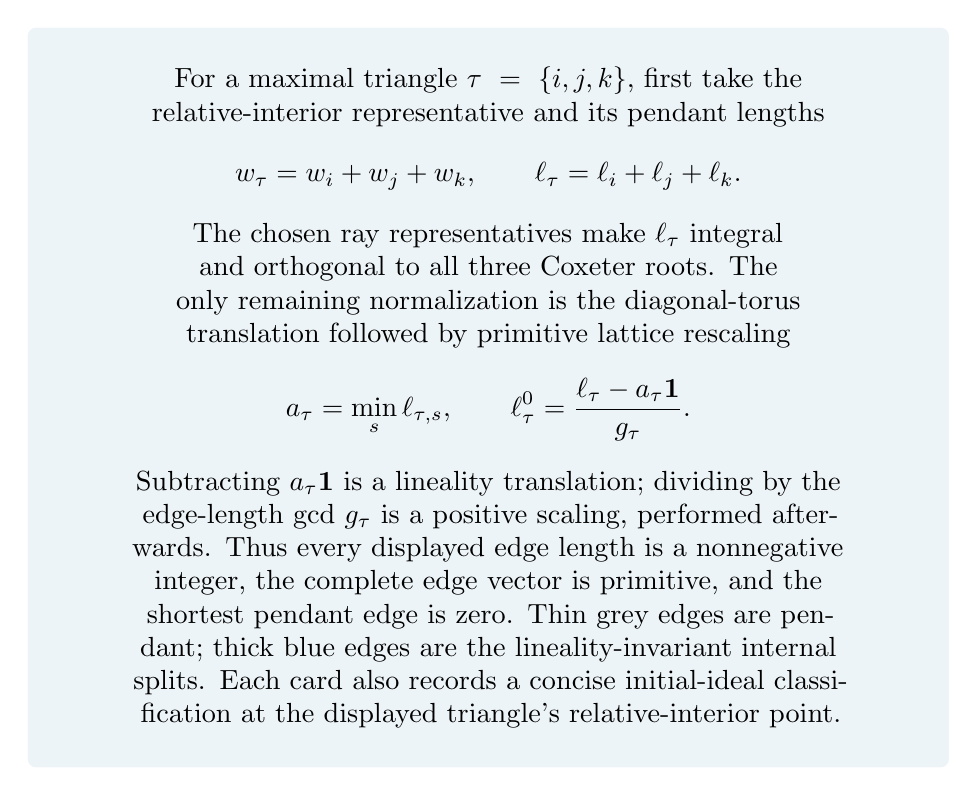
\begin{tikzpicture}
    \node[rounded corners=3pt,fill=paperblue,inner xsep=10mm,inner ysep=5mm,
          text width=.80\textwidth,align=center] {
      For a maximal triangle $\tau=\{i,j,k\}$, first take the relative-interior
      representative and its pendant lengths
      \[
        w_\tau=w_i+w_j+w_k,\qquad
        \ell_\tau=\ell_i+\ell_j+\ell_k.
      \]
      The chosen ray representatives make $\ell_\tau$ integral and orthogonal
      to all three Coxeter roots. The only remaining normalization is the
      diagonal-torus translation followed by primitive lattice rescaling
      \[
        a_\tau=\min_s\ell_{\tau,s},\qquad
        \ell_\tau^0=\frac{\ell_\tau-a_\tau\mathbf 1}{g_\tau}.
      \]
      Subtracting $a_\tau\mathbf 1$ is a lineality translation; dividing by
      the edge-length gcd $g_\tau$ is a positive scaling, performed afterwards.
      Thus every displayed edge length is a nonnegative integer, the complete
      edge vector is primitive, and the shortest pendant edge is zero. Thin
      grey edges are pendant; thick blue edges are the lineality-invariant
      internal splits. Each card also records a concise initial-ideal
      classification at the displayed triangle's relative-interior point.
    };
  \end{tikzpicture}
\end{center}
\vfill
\begin{center}\color{muted}
The 251 triangles form 24 combinatorial facet orbits. Taxon $7$ is the
rust-colored top vertex of each regular heptagon; internal vertices use a
harmonic layout.\\[1mm]
Orbit sizes: \(12,\,24,\,24,\,12,\,12,\,12,\,24,\,24,\,12,\,12,\,12,\,12,\,3,\,3,\,12,\,3,\,3,\,6,\,6,\,3,\,6,\,6,\,6,\,2\).
\\[1mm]{\textcolor{toricgreen}{\bfseries 135 prime toric}}\quad{\textcolor{warningamber}{\bfseries 2 prime non-binomial}}\quad{\textcolor{nonprimered}{\bfseries 114 non-prime}}.
\\[1mm]{\scriptsize On each card, `GB \(a/b\)' means \(a\) reduced Gr\"obner-basis elements and at most \(b\) terms per element; for a Newton--Okounkov body, `degree-one/lattice' compares distinct Pl\"ucker values with all lattice points.}
\end{center}
\clearpage

\begin{tikzpicture}
\node[rounded corners=2pt,fill=paperblue,inner xsep=5mm,inner ysep=2mm,text width=.94\textwidth] {\Large\bfseries Orbit 1\hfill\normalsize 12 triangles};
\end{tikzpicture}\par\vspace{0.5mm}
{\scriptsize\color{muted} Triangle indices: 1, 2, 49, 50, 154, 155, 182, 183, 192, 193, 248, 249}\par{\scriptsize\color{muted} Algebra: \textcolor{toricgreen}{12 toric}, \textcolor{warningamber}{0 prime non-binomial}, \textcolor{nonprimered}{0 non-prime}.}\par\vspace{1mm}
\begin{minipage}[t][0.225\textheight][t]{0.485\textwidth}
\centering
{\normalsize\bfseries Triangle 1}\par
{\small\color{muted} Rays $\{1,\,2,\,3\}$}\par\vspace{0.3mm}
{\scriptsize \textcolor{toricgreen}{\bfseries PRIME TORIC}\color{muted}\quad $\dim/\deg=6/18$\quad GB 35/2}\par
{\scriptsize\color{bodyviolet} $f=(9,\,27,\,38,\,27,\,9)$\quad degree-one/lattice $=14/14$}\par\vspace{0.3mm}
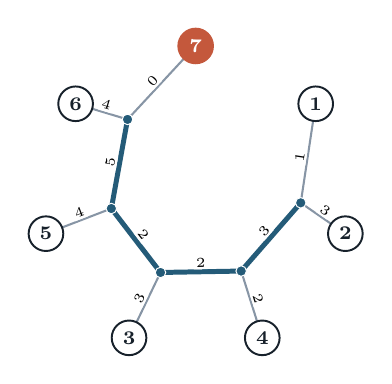
\begin{tikzpicture}[x=1cm,y=1cm]
\coordinate (v1) at (1.52457,1.21581);
\coordinate (v2) at (1.90111,-0.43392);
\coordinate (v3) at (-0.84607,-1.75689);
\coordinate (v4) at (0.84607,-1.75689);
\coordinate (v5) at (-1.90111,-0.43392);
\coordinate (v6) at (-1.52457,1.21581);
\coordinate (v7) at (0.00000,1.95000);
\coordinate (v8) at (-0.86513,1.01711);
\coordinate (v9) at (1.33461,-0.04223);
\coordinate (v10) at (0.57814,-0.90859);
\coordinate (v11) at (-0.44625,-0.92666);
\coordinate (v12) at (-1.07083,-0.11449);
\draw[internal edge] (v8) -- node[edge label,pos=0.50] {$5$} (v12);
\draw[internal edge] (v9) -- node[edge label,pos=0.50] {$3$} (v10);
\draw[internal edge] (v10) -- node[edge label,pos=0.50] {$2$} (v11);
\draw[internal edge] (v11) -- node[edge label,pos=0.50] {$2$} (v12);
\draw[pendant edge] (v1) -- node[edge label,pos=0.55] {$1$} (v9);
\draw[pendant edge] (v2) -- node[edge label,pos=0.55] {$3$} (v9);
\draw[pendant edge] (v3) -- node[edge label,pos=0.55] {$3$} (v11);
\draw[pendant edge] (v4) -- node[edge label,pos=0.55] {$2$} (v10);
\draw[pendant edge] (v5) -- node[edge label,pos=0.55] {$4$} (v12);
\draw[pendant edge] (v6) -- node[edge label,pos=0.55] {$4$} (v8);
\draw[pendant edge] (v7) -- node[edge label,pos=0.55] {$0$} (v8);
\node[internal vertex] at (v8) {};
\node[internal vertex] at (v9) {};
\node[internal vertex] at (v10) {};
\node[internal vertex] at (v11) {};
\node[internal vertex] at (v12) {};
\node[leaf] at (v1) {1};
\node[leaf] at (v2) {2};
\node[leaf] at (v3) {3};
\node[leaf] at (v4) {4};
\node[leaf] at (v5) {5};
\node[leaf] at (v6) {6};
\node[special leaf] at (v7) {7};
\end{tikzpicture}
\end{minipage}
\hfill
\begin{minipage}[t][0.225\textheight][t]{0.485\textwidth}
\centering
{\normalsize\bfseries Triangle 2}\par
{\small\color{muted} Rays $\{2,\,4,\,5\}$}\par\vspace{0.3mm}
{\scriptsize \textcolor{toricgreen}{\bfseries PRIME TORIC}\color{muted}\quad $\dim/\deg=6/18$\quad GB 35/2}\par
{\scriptsize\color{bodyviolet} $f=(9,\,27,\,38,\,27,\,9)$\quad degree-one/lattice $=14/14$}\par\vspace{0.3mm}
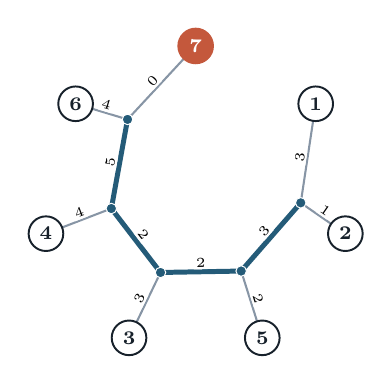
\begin{tikzpicture}[x=1cm,y=1cm]
\coordinate (v1) at (1.52457,1.21581);
\coordinate (v2) at (1.90111,-0.43392);
\coordinate (v3) at (-0.84607,-1.75689);
\coordinate (v4) at (-1.90111,-0.43392);
\coordinate (v5) at (0.84607,-1.75689);
\coordinate (v6) at (-1.52457,1.21581);
\coordinate (v7) at (0.00000,1.95000);
\coordinate (v8) at (-0.86513,1.01711);
\coordinate (v9) at (1.33461,-0.04223);
\coordinate (v10) at (-1.07083,-0.11449);
\coordinate (v11) at (-0.44625,-0.92666);
\coordinate (v12) at (0.57814,-0.90859);
\draw[internal edge] (v8) -- node[edge label,pos=0.50] {$5$} (v10);
\draw[internal edge] (v9) -- node[edge label,pos=0.50] {$3$} (v12);
\draw[internal edge] (v10) -- node[edge label,pos=0.50] {$2$} (v11);
\draw[internal edge] (v11) -- node[edge label,pos=0.50] {$2$} (v12);
\draw[pendant edge] (v1) -- node[edge label,pos=0.55] {$3$} (v9);
\draw[pendant edge] (v2) -- node[edge label,pos=0.55] {$1$} (v9);
\draw[pendant edge] (v3) -- node[edge label,pos=0.55] {$3$} (v11);
\draw[pendant edge] (v4) -- node[edge label,pos=0.55] {$4$} (v10);
\draw[pendant edge] (v5) -- node[edge label,pos=0.55] {$2$} (v12);
\draw[pendant edge] (v6) -- node[edge label,pos=0.55] {$4$} (v8);
\draw[pendant edge] (v7) -- node[edge label,pos=0.55] {$0$} (v8);
\node[internal vertex] at (v8) {};
\node[internal vertex] at (v9) {};
\node[internal vertex] at (v10) {};
\node[internal vertex] at (v11) {};
\node[internal vertex] at (v12) {};
\node[leaf] at (v1) {1};
\node[leaf] at (v2) {2};
\node[leaf] at (v3) {3};
\node[leaf] at (v4) {4};
\node[leaf] at (v5) {5};
\node[leaf] at (v6) {6};
\node[special leaf] at (v7) {7};
\end{tikzpicture}
\end{minipage}
\par
\begin{minipage}[t][0.225\textheight][t]{0.485\textwidth}
\centering
{\normalsize\bfseries Triangle 49}\par
{\small\color{muted} Rays $\{3,\,23,\,25\}$}\par\vspace{0.3mm}
{\scriptsize \textcolor{toricgreen}{\bfseries PRIME TORIC}\color{muted}\quad $\dim/\deg=6/18$\quad GB 37/2}\par
{\scriptsize\color{bodyviolet} $f=(9,\,27,\,38,\,27,\,9)$\quad degree-one/lattice $=14/14$}\par\vspace{0.3mm}
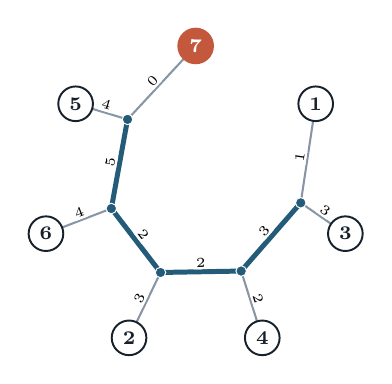
\begin{tikzpicture}[x=1cm,y=1cm]
\coordinate (v1) at (1.52457,1.21581);
\coordinate (v2) at (-0.84607,-1.75689);
\coordinate (v3) at (1.90111,-0.43392);
\coordinate (v4) at (0.84607,-1.75689);
\coordinate (v5) at (-1.52457,1.21581);
\coordinate (v6) at (-1.90111,-0.43392);
\coordinate (v7) at (0.00000,1.95000);
\coordinate (v8) at (-0.86513,1.01711);
\coordinate (v9) at (1.33461,-0.04223);
\coordinate (v10) at (0.57814,-0.90859);
\coordinate (v11) at (-0.44625,-0.92666);
\coordinate (v12) at (-1.07083,-0.11449);
\draw[internal edge] (v8) -- node[edge label,pos=0.50] {$5$} (v12);
\draw[internal edge] (v9) -- node[edge label,pos=0.50] {$3$} (v10);
\draw[internal edge] (v10) -- node[edge label,pos=0.50] {$2$} (v11);
\draw[internal edge] (v11) -- node[edge label,pos=0.50] {$2$} (v12);
\draw[pendant edge] (v1) -- node[edge label,pos=0.55] {$1$} (v9);
\draw[pendant edge] (v2) -- node[edge label,pos=0.55] {$3$} (v11);
\draw[pendant edge] (v3) -- node[edge label,pos=0.55] {$3$} (v9);
\draw[pendant edge] (v4) -- node[edge label,pos=0.55] {$2$} (v10);
\draw[pendant edge] (v5) -- node[edge label,pos=0.55] {$4$} (v8);
\draw[pendant edge] (v6) -- node[edge label,pos=0.55] {$4$} (v12);
\draw[pendant edge] (v7) -- node[edge label,pos=0.55] {$0$} (v8);
\node[internal vertex] at (v8) {};
\node[internal vertex] at (v9) {};
\node[internal vertex] at (v10) {};
\node[internal vertex] at (v11) {};
\node[internal vertex] at (v12) {};
\node[leaf] at (v1) {1};
\node[leaf] at (v2) {2};
\node[leaf] at (v3) {3};
\node[leaf] at (v4) {4};
\node[leaf] at (v5) {5};
\node[leaf] at (v6) {6};
\node[special leaf] at (v7) {7};
\end{tikzpicture}
\end{minipage}
\hfill
\begin{minipage}[t][0.225\textheight][t]{0.485\textwidth}
\centering
{\normalsize\bfseries Triangle 50}\par
{\small\color{muted} Rays $\{5,\,24,\,26\}$}\par\vspace{0.3mm}
{\scriptsize \textcolor{toricgreen}{\bfseries PRIME TORIC}\color{muted}\quad $\dim/\deg=6/18$\quad GB 35/2}\par
{\scriptsize\color{bodyviolet} $f=(9,\,27,\,38,\,27,\,9)$\quad degree-one/lattice $=14/14$}\par\vspace{0.3mm}
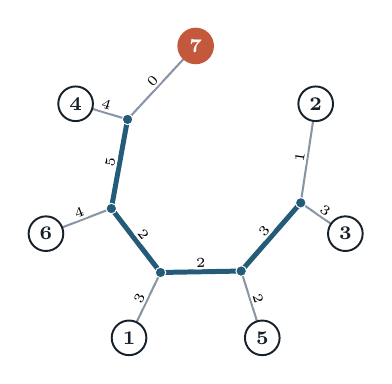
\begin{tikzpicture}[x=1cm,y=1cm]
\coordinate (v1) at (-0.84607,-1.75689);
\coordinate (v2) at (1.52457,1.21581);
\coordinate (v3) at (1.90111,-0.43392);
\coordinate (v4) at (-1.52457,1.21581);
\coordinate (v5) at (0.84607,-1.75689);
\coordinate (v6) at (-1.90111,-0.43392);
\coordinate (v7) at (0.00000,1.95000);
\coordinate (v8) at (-0.86513,1.01711);
\coordinate (v9) at (1.33461,-0.04223);
\coordinate (v10) at (0.57814,-0.90859);
\coordinate (v11) at (-0.44625,-0.92666);
\coordinate (v12) at (-1.07083,-0.11449);
\draw[internal edge] (v8) -- node[edge label,pos=0.50] {$5$} (v12);
\draw[internal edge] (v9) -- node[edge label,pos=0.50] {$3$} (v10);
\draw[internal edge] (v10) -- node[edge label,pos=0.50] {$2$} (v11);
\draw[internal edge] (v11) -- node[edge label,pos=0.50] {$2$} (v12);
\draw[pendant edge] (v1) -- node[edge label,pos=0.55] {$3$} (v11);
\draw[pendant edge] (v2) -- node[edge label,pos=0.55] {$1$} (v9);
\draw[pendant edge] (v3) -- node[edge label,pos=0.55] {$3$} (v9);
\draw[pendant edge] (v4) -- node[edge label,pos=0.55] {$4$} (v8);
\draw[pendant edge] (v5) -- node[edge label,pos=0.55] {$2$} (v10);
\draw[pendant edge] (v6) -- node[edge label,pos=0.55] {$4$} (v12);
\draw[pendant edge] (v7) -- node[edge label,pos=0.55] {$0$} (v8);
\node[internal vertex] at (v8) {};
\node[internal vertex] at (v9) {};
\node[internal vertex] at (v10) {};
\node[internal vertex] at (v11) {};
\node[internal vertex] at (v12) {};
\node[leaf] at (v1) {1};
\node[leaf] at (v2) {2};
\node[leaf] at (v3) {3};
\node[leaf] at (v4) {4};
\node[leaf] at (v5) {5};
\node[leaf] at (v6) {6};
\node[special leaf] at (v7) {7};
\end{tikzpicture}
\end{minipage}
\par
\begin{minipage}[t][0.225\textheight][t]{0.485\textwidth}
\centering
{\normalsize\bfseries Triangle 154}\par
{\small\color{muted} Rays $\{16,\,32,\,38\}$}\par\vspace{0.3mm}
{\scriptsize \textcolor{toricgreen}{\bfseries PRIME TORIC}\color{muted}\quad $\dim/\deg=6/18$\quad GB 41/2}\par
{\scriptsize\color{bodyviolet} $f=(9,\,27,\,38,\,27,\,9)$\quad degree-one/lattice $=14/14$}\par\vspace{0.3mm}
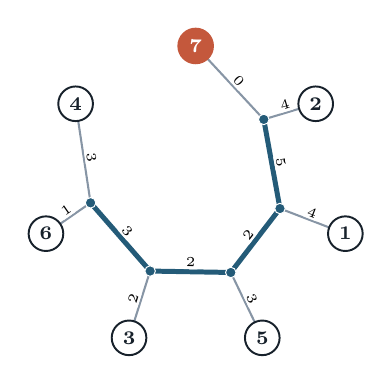
\begin{tikzpicture}[x=1cm,y=1cm]
\coordinate (v1) at (1.90111,-0.43392);
\coordinate (v2) at (1.52457,1.21581);
\coordinate (v3) at (-0.84607,-1.75689);
\coordinate (v4) at (-1.52457,1.21581);
\coordinate (v5) at (0.84607,-1.75689);
\coordinate (v6) at (-1.90111,-0.43392);
\coordinate (v7) at (0.00000,1.95000);
\coordinate (v8) at (0.86513,1.01711);
\coordinate (v9) at (-1.33461,-0.04223);
\coordinate (v10) at (1.07083,-0.11449);
\coordinate (v11) at (-0.57814,-0.90859);
\coordinate (v12) at (0.44625,-0.92666);
\draw[internal edge] (v8) -- node[edge label,pos=0.50] {$5$} (v10);
\draw[internal edge] (v9) -- node[edge label,pos=0.50] {$3$} (v11);
\draw[internal edge] (v10) -- node[edge label,pos=0.50] {$2$} (v12);
\draw[internal edge] (v11) -- node[edge label,pos=0.50] {$2$} (v12);
\draw[pendant edge] (v1) -- node[edge label,pos=0.55] {$4$} (v10);
\draw[pendant edge] (v2) -- node[edge label,pos=0.55] {$4$} (v8);
\draw[pendant edge] (v3) -- node[edge label,pos=0.55] {$2$} (v11);
\draw[pendant edge] (v4) -- node[edge label,pos=0.55] {$3$} (v9);
\draw[pendant edge] (v5) -- node[edge label,pos=0.55] {$3$} (v12);
\draw[pendant edge] (v6) -- node[edge label,pos=0.55] {$1$} (v9);
\draw[pendant edge] (v7) -- node[edge label,pos=0.55] {$0$} (v8);
\node[internal vertex] at (v8) {};
\node[internal vertex] at (v9) {};
\node[internal vertex] at (v10) {};
\node[internal vertex] at (v11) {};
\node[internal vertex] at (v12) {};
\node[leaf] at (v1) {1};
\node[leaf] at (v2) {2};
\node[leaf] at (v3) {3};
\node[leaf] at (v4) {4};
\node[leaf] at (v5) {5};
\node[leaf] at (v6) {6};
\node[special leaf] at (v7) {7};
\end{tikzpicture}
\end{minipage}
\hfill
\begin{minipage}[t][0.225\textheight][t]{0.485\textwidth}
\centering
{\normalsize\bfseries Triangle 155}\par
{\small\color{muted} Rays $\{16,\,31,\,39\}$}\par\vspace{0.3mm}
{\scriptsize \textcolor{toricgreen}{\bfseries PRIME TORIC}\color{muted}\quad $\dim/\deg=6/18$\quad GB 40/2}\par
{\scriptsize\color{bodyviolet} $f=(9,\,27,\,38,\,27,\,9)$\quad degree-one/lattice $=14/14$}\par\vspace{0.3mm}
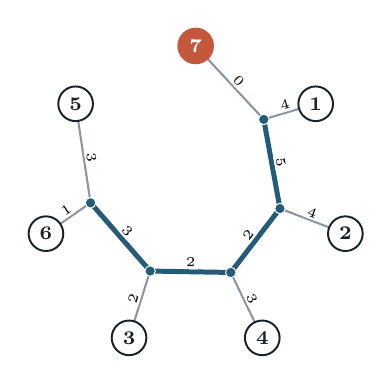
\begin{tikzpicture}[x=1cm,y=1cm]
\coordinate (v1) at (1.52457,1.21581);
\coordinate (v2) at (1.90111,-0.43392);
\coordinate (v3) at (-0.84607,-1.75689);
\coordinate (v4) at (0.84607,-1.75689);
\coordinate (v5) at (-1.52457,1.21581);
\coordinate (v6) at (-1.90111,-0.43392);
\coordinate (v7) at (0.00000,1.95000);
\coordinate (v8) at (0.86513,1.01711);
\coordinate (v9) at (-1.33461,-0.04223);
\coordinate (v10) at (1.07083,-0.11449);
\coordinate (v11) at (-0.57814,-0.90859);
\coordinate (v12) at (0.44625,-0.92666);
\draw[internal edge] (v8) -- node[edge label,pos=0.50] {$5$} (v10);
\draw[internal edge] (v9) -- node[edge label,pos=0.50] {$3$} (v11);
\draw[internal edge] (v10) -- node[edge label,pos=0.50] {$2$} (v12);
\draw[internal edge] (v11) -- node[edge label,pos=0.50] {$2$} (v12);
\draw[pendant edge] (v1) -- node[edge label,pos=0.55] {$4$} (v8);
\draw[pendant edge] (v2) -- node[edge label,pos=0.55] {$4$} (v10);
\draw[pendant edge] (v3) -- node[edge label,pos=0.55] {$2$} (v11);
\draw[pendant edge] (v4) -- node[edge label,pos=0.55] {$3$} (v12);
\draw[pendant edge] (v5) -- node[edge label,pos=0.55] {$3$} (v9);
\draw[pendant edge] (v6) -- node[edge label,pos=0.55] {$1$} (v9);
\draw[pendant edge] (v7) -- node[edge label,pos=0.55] {$0$} (v8);
\node[internal vertex] at (v8) {};
\node[internal vertex] at (v9) {};
\node[internal vertex] at (v10) {};
\node[internal vertex] at (v11) {};
\node[internal vertex] at (v12) {};
\node[leaf] at (v1) {1};
\node[leaf] at (v2) {2};
\node[leaf] at (v3) {3};
\node[leaf] at (v4) {4};
\node[leaf] at (v5) {5};
\node[leaf] at (v6) {6};
\node[special leaf] at (v7) {7};
\end{tikzpicture}
\end{minipage}
\par
\begin{minipage}[t][0.225\textheight][t]{0.485\textwidth}
\centering
{\normalsize\bfseries Triangle 182}\par
{\small\color{muted} Rays $\{25,\,27,\,48\}$}\par\vspace{0.3mm}
{\scriptsize \textcolor{toricgreen}{\bfseries PRIME TORIC}\color{muted}\quad $\dim/\deg=6/18$\quad GB 36/2}\par
{\scriptsize\color{bodyviolet} $f=(9,\,27,\,38,\,27,\,9)$\quad degree-one/lattice $=14/14$}\par\vspace{0.3mm}
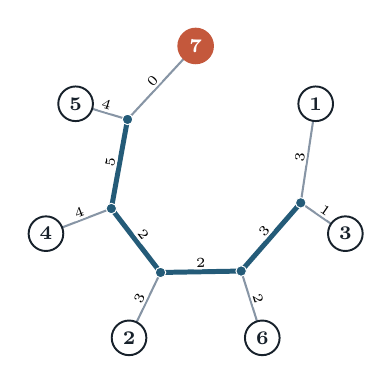
\begin{tikzpicture}[x=1cm,y=1cm]
\coordinate (v1) at (1.52457,1.21581);
\coordinate (v2) at (-0.84607,-1.75689);
\coordinate (v3) at (1.90111,-0.43392);
\coordinate (v4) at (-1.90111,-0.43392);
\coordinate (v5) at (-1.52457,1.21581);
\coordinate (v6) at (0.84607,-1.75689);
\coordinate (v7) at (0.00000,1.95000);
\coordinate (v8) at (-0.86513,1.01711);
\coordinate (v9) at (1.33461,-0.04223);
\coordinate (v10) at (-1.07083,-0.11449);
\coordinate (v11) at (-0.44625,-0.92666);
\coordinate (v12) at (0.57814,-0.90859);
\draw[internal edge] (v8) -- node[edge label,pos=0.50] {$5$} (v10);
\draw[internal edge] (v9) -- node[edge label,pos=0.50] {$3$} (v12);
\draw[internal edge] (v10) -- node[edge label,pos=0.50] {$2$} (v11);
\draw[internal edge] (v11) -- node[edge label,pos=0.50] {$2$} (v12);
\draw[pendant edge] (v1) -- node[edge label,pos=0.55] {$3$} (v9);
\draw[pendant edge] (v2) -- node[edge label,pos=0.55] {$3$} (v11);
\draw[pendant edge] (v3) -- node[edge label,pos=0.55] {$1$} (v9);
\draw[pendant edge] (v4) -- node[edge label,pos=0.55] {$4$} (v10);
\draw[pendant edge] (v5) -- node[edge label,pos=0.55] {$4$} (v8);
\draw[pendant edge] (v6) -- node[edge label,pos=0.55] {$2$} (v12);
\draw[pendant edge] (v7) -- node[edge label,pos=0.55] {$0$} (v8);
\node[internal vertex] at (v8) {};
\node[internal vertex] at (v9) {};
\node[internal vertex] at (v10) {};
\node[internal vertex] at (v11) {};
\node[internal vertex] at (v12) {};
\node[leaf] at (v1) {1};
\node[leaf] at (v2) {2};
\node[leaf] at (v3) {3};
\node[leaf] at (v4) {4};
\node[leaf] at (v5) {5};
\node[leaf] at (v6) {6};
\node[special leaf] at (v7) {7};
\end{tikzpicture}
\end{minipage}
\hfill
\begin{minipage}[t][0.225\textheight][t]{0.485\textwidth}
\centering
{\normalsize\bfseries Triangle 183}\par
{\small\color{muted} Rays $\{26,\,27,\,49\}$}\par\vspace{0.3mm}
{\scriptsize \textcolor{toricgreen}{\bfseries PRIME TORIC}\color{muted}\quad $\dim/\deg=6/18$\quad GB 36/2}\par
{\scriptsize\color{bodyviolet} $f=(9,\,27,\,38,\,27,\,9)$\quad degree-one/lattice $=14/14$}\par\vspace{0.3mm}
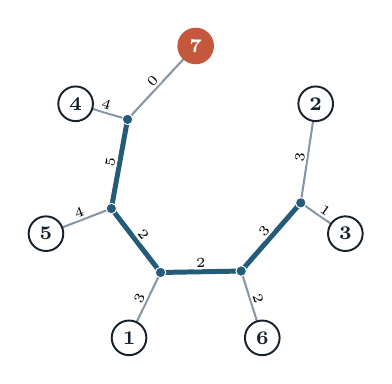
\begin{tikzpicture}[x=1cm,y=1cm]
\coordinate (v1) at (-0.84607,-1.75689);
\coordinate (v2) at (1.52457,1.21581);
\coordinate (v3) at (1.90111,-0.43392);
\coordinate (v4) at (-1.52457,1.21581);
\coordinate (v5) at (-1.90111,-0.43392);
\coordinate (v6) at (0.84607,-1.75689);
\coordinate (v7) at (0.00000,1.95000);
\coordinate (v8) at (-0.86513,1.01711);
\coordinate (v9) at (1.33461,-0.04223);
\coordinate (v10) at (-1.07083,-0.11449);
\coordinate (v11) at (-0.44625,-0.92666);
\coordinate (v12) at (0.57814,-0.90859);
\draw[internal edge] (v8) -- node[edge label,pos=0.50] {$5$} (v10);
\draw[internal edge] (v9) -- node[edge label,pos=0.50] {$3$} (v12);
\draw[internal edge] (v10) -- node[edge label,pos=0.50] {$2$} (v11);
\draw[internal edge] (v11) -- node[edge label,pos=0.50] {$2$} (v12);
\draw[pendant edge] (v1) -- node[edge label,pos=0.55] {$3$} (v11);
\draw[pendant edge] (v2) -- node[edge label,pos=0.55] {$3$} (v9);
\draw[pendant edge] (v3) -- node[edge label,pos=0.55] {$1$} (v9);
\draw[pendant edge] (v4) -- node[edge label,pos=0.55] {$4$} (v8);
\draw[pendant edge] (v5) -- node[edge label,pos=0.55] {$4$} (v10);
\draw[pendant edge] (v6) -- node[edge label,pos=0.55] {$2$} (v12);
\draw[pendant edge] (v7) -- node[edge label,pos=0.55] {$0$} (v8);
\node[internal vertex] at (v8) {};
\node[internal vertex] at (v9) {};
\node[internal vertex] at (v10) {};
\node[internal vertex] at (v11) {};
\node[internal vertex] at (v12) {};
\node[leaf] at (v1) {1};
\node[leaf] at (v2) {2};
\node[leaf] at (v3) {3};
\node[leaf] at (v4) {4};
\node[leaf] at (v5) {5};
\node[leaf] at (v6) {6};
\node[special leaf] at (v7) {7};
\end{tikzpicture}
\end{minipage}
\par
\clearpage

\begin{tikzpicture}
\node[rounded corners=2pt,fill=paperblue,inner xsep=5mm,inner ysep=2mm,text width=.94\textwidth] {\Large\bfseries Orbit 1 (continued)\hfill\normalsize 12 triangles};
\end{tikzpicture}\par\vspace{0.5mm}
{\scriptsize\color{muted} Triangle indices: 1, 2, 49, 50, 154, 155, 182, 183, 192, 193, 248, 249}\par{\scriptsize\color{muted} Algebra: \textcolor{toricgreen}{12 toric}, \textcolor{warningamber}{0 prime non-binomial}, \textcolor{nonprimered}{0 non-prime}.}\par\vspace{1mm}
\begin{minipage}[t][0.225\textheight][t]{0.485\textwidth}
\centering
{\normalsize\bfseries Triangle 192}\par
{\small\color{muted} Rays $\{28,\,42,\,46\}$}\par\vspace{0.3mm}
{\scriptsize \textcolor{toricgreen}{\bfseries PRIME TORIC}\color{muted}\quad $\dim/\deg=6/18$\quad GB 37/2}\par
{\scriptsize\color{bodyviolet} $f=(9,\,27,\,38,\,27,\,9)$\quad degree-one/lattice $=14/14$}\par\vspace{0.3mm}
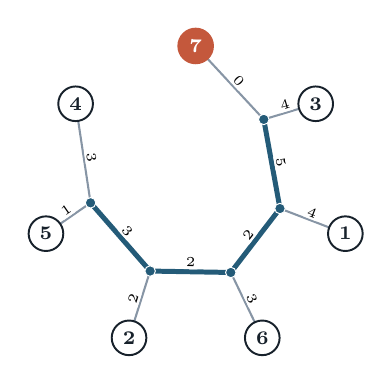
\begin{tikzpicture}[x=1cm,y=1cm]
\coordinate (v1) at (1.90111,-0.43392);
\coordinate (v2) at (-0.84607,-1.75689);
\coordinate (v3) at (1.52457,1.21581);
\coordinate (v4) at (-1.52457,1.21581);
\coordinate (v5) at (-1.90111,-0.43392);
\coordinate (v6) at (0.84607,-1.75689);
\coordinate (v7) at (0.00000,1.95000);
\coordinate (v8) at (0.86513,1.01711);
\coordinate (v9) at (-1.33461,-0.04223);
\coordinate (v10) at (1.07083,-0.11449);
\coordinate (v11) at (-0.57814,-0.90859);
\coordinate (v12) at (0.44625,-0.92666);
\draw[internal edge] (v8) -- node[edge label,pos=0.50] {$5$} (v10);
\draw[internal edge] (v9) -- node[edge label,pos=0.50] {$3$} (v11);
\draw[internal edge] (v10) -- node[edge label,pos=0.50] {$2$} (v12);
\draw[internal edge] (v11) -- node[edge label,pos=0.50] {$2$} (v12);
\draw[pendant edge] (v1) -- node[edge label,pos=0.55] {$4$} (v10);
\draw[pendant edge] (v2) -- node[edge label,pos=0.55] {$2$} (v11);
\draw[pendant edge] (v3) -- node[edge label,pos=0.55] {$4$} (v8);
\draw[pendant edge] (v4) -- node[edge label,pos=0.55] {$3$} (v9);
\draw[pendant edge] (v5) -- node[edge label,pos=0.55] {$1$} (v9);
\draw[pendant edge] (v6) -- node[edge label,pos=0.55] {$3$} (v12);
\draw[pendant edge] (v7) -- node[edge label,pos=0.55] {$0$} (v8);
\node[internal vertex] at (v8) {};
\node[internal vertex] at (v9) {};
\node[internal vertex] at (v10) {};
\node[internal vertex] at (v11) {};
\node[internal vertex] at (v12) {};
\node[leaf] at (v1) {1};
\node[leaf] at (v2) {2};
\node[leaf] at (v3) {3};
\node[leaf] at (v4) {4};
\node[leaf] at (v5) {5};
\node[leaf] at (v6) {6};
\node[special leaf] at (v7) {7};
\end{tikzpicture}
\end{minipage}
\hfill
\begin{minipage}[t][0.225\textheight][t]{0.485\textwidth}
\centering
{\normalsize\bfseries Triangle 193}\par
{\small\color{muted} Rays $\{28,\,43,\,47\}$}\par\vspace{0.3mm}
{\scriptsize \textcolor{toricgreen}{\bfseries PRIME TORIC}\color{muted}\quad $\dim/\deg=6/18$\quad GB 35/2}\par
{\scriptsize\color{bodyviolet} $f=(9,\,27,\,38,\,27,\,9)$\quad degree-one/lattice $=14/14$}\par\vspace{0.3mm}
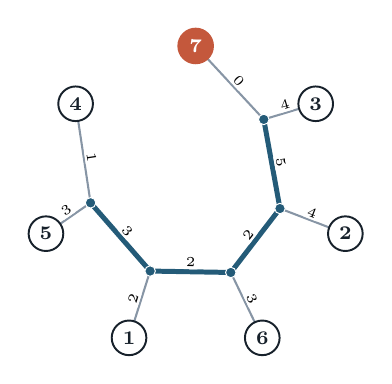
\begin{tikzpicture}[x=1cm,y=1cm]
\coordinate (v1) at (-0.84607,-1.75689);
\coordinate (v2) at (1.90111,-0.43392);
\coordinate (v3) at (1.52457,1.21581);
\coordinate (v4) at (-1.52457,1.21581);
\coordinate (v5) at (-1.90111,-0.43392);
\coordinate (v6) at (0.84607,-1.75689);
\coordinate (v7) at (0.00000,1.95000);
\coordinate (v8) at (0.86513,1.01711);
\coordinate (v9) at (-1.33461,-0.04223);
\coordinate (v10) at (-0.57814,-0.90859);
\coordinate (v11) at (1.07083,-0.11449);
\coordinate (v12) at (0.44625,-0.92666);
\draw[internal edge] (v8) -- node[edge label,pos=0.50] {$5$} (v11);
\draw[internal edge] (v9) -- node[edge label,pos=0.50] {$3$} (v10);
\draw[internal edge] (v10) -- node[edge label,pos=0.50] {$2$} (v12);
\draw[internal edge] (v11) -- node[edge label,pos=0.50] {$2$} (v12);
\draw[pendant edge] (v1) -- node[edge label,pos=0.55] {$2$} (v10);
\draw[pendant edge] (v2) -- node[edge label,pos=0.55] {$4$} (v11);
\draw[pendant edge] (v3) -- node[edge label,pos=0.55] {$4$} (v8);
\draw[pendant edge] (v4) -- node[edge label,pos=0.55] {$1$} (v9);
\draw[pendant edge] (v5) -- node[edge label,pos=0.55] {$3$} (v9);
\draw[pendant edge] (v6) -- node[edge label,pos=0.55] {$3$} (v12);
\draw[pendant edge] (v7) -- node[edge label,pos=0.55] {$0$} (v8);
\node[internal vertex] at (v8) {};
\node[internal vertex] at (v9) {};
\node[internal vertex] at (v10) {};
\node[internal vertex] at (v11) {};
\node[internal vertex] at (v12) {};
\node[leaf] at (v1) {1};
\node[leaf] at (v2) {2};
\node[leaf] at (v3) {3};
\node[leaf] at (v4) {4};
\node[leaf] at (v5) {5};
\node[leaf] at (v6) {6};
\node[special leaf] at (v7) {7};
\end{tikzpicture}
\end{minipage}
\par
\begin{minipage}[t][0.225\textheight][t]{0.485\textwidth}
\centering
{\normalsize\bfseries Triangle 248}\par
{\small\color{muted} Rays $\{31,\,46,\,51\}$}\par\vspace{0.3mm}
{\scriptsize \textcolor{toricgreen}{\bfseries PRIME TORIC}\color{muted}\quad $\dim/\deg=6/18$\quad GB 42/2}\par
{\scriptsize\color{bodyviolet} $f=(9,\,27,\,38,\,27,\,9)$\quad degree-one/lattice $=14/14$}\par\vspace{0.3mm}
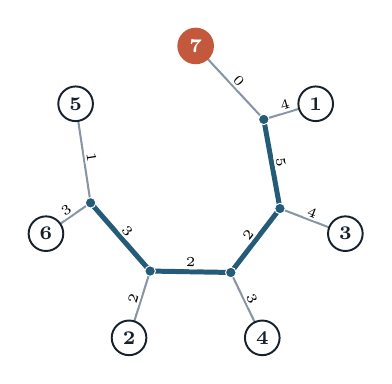
\begin{tikzpicture}[x=1cm,y=1cm]
\coordinate (v1) at (1.52457,1.21581);
\coordinate (v2) at (-0.84607,-1.75689);
\coordinate (v3) at (1.90111,-0.43392);
\coordinate (v4) at (0.84607,-1.75689);
\coordinate (v5) at (-1.52457,1.21581);
\coordinate (v6) at (-1.90111,-0.43392);
\coordinate (v7) at (0.00000,1.95000);
\coordinate (v8) at (0.86513,1.01711);
\coordinate (v9) at (-1.33461,-0.04223);
\coordinate (v10) at (-0.57814,-0.90859);
\coordinate (v11) at (1.07083,-0.11449);
\coordinate (v12) at (0.44625,-0.92666);
\draw[internal edge] (v8) -- node[edge label,pos=0.50] {$5$} (v11);
\draw[internal edge] (v9) -- node[edge label,pos=0.50] {$3$} (v10);
\draw[internal edge] (v10) -- node[edge label,pos=0.50] {$2$} (v12);
\draw[internal edge] (v11) -- node[edge label,pos=0.50] {$2$} (v12);
\draw[pendant edge] (v1) -- node[edge label,pos=0.55] {$4$} (v8);
\draw[pendant edge] (v2) -- node[edge label,pos=0.55] {$2$} (v10);
\draw[pendant edge] (v3) -- node[edge label,pos=0.55] {$4$} (v11);
\draw[pendant edge] (v4) -- node[edge label,pos=0.55] {$3$} (v12);
\draw[pendant edge] (v5) -- node[edge label,pos=0.55] {$1$} (v9);
\draw[pendant edge] (v6) -- node[edge label,pos=0.55] {$3$} (v9);
\draw[pendant edge] (v7) -- node[edge label,pos=0.55] {$0$} (v8);
\node[internal vertex] at (v8) {};
\node[internal vertex] at (v9) {};
\node[internal vertex] at (v10) {};
\node[internal vertex] at (v11) {};
\node[internal vertex] at (v12) {};
\node[leaf] at (v1) {1};
\node[leaf] at (v2) {2};
\node[leaf] at (v3) {3};
\node[leaf] at (v4) {4};
\node[leaf] at (v5) {5};
\node[leaf] at (v6) {6};
\node[special leaf] at (v7) {7};
\end{tikzpicture}
\end{minipage}
\hfill
\begin{minipage}[t][0.225\textheight][t]{0.485\textwidth}
\centering
{\normalsize\bfseries Triangle 249}\par
{\small\color{muted} Rays $\{32,\,47,\,50\}$}\par\vspace{0.3mm}
{\scriptsize \textcolor{toricgreen}{\bfseries PRIME TORIC}\color{muted}\quad $\dim/\deg=6/18$\quad GB 40/2}\par
{\scriptsize\color{bodyviolet} $f=(9,\,27,\,38,\,27,\,9)$\quad degree-one/lattice $=14/14$}\par\vspace{0.3mm}
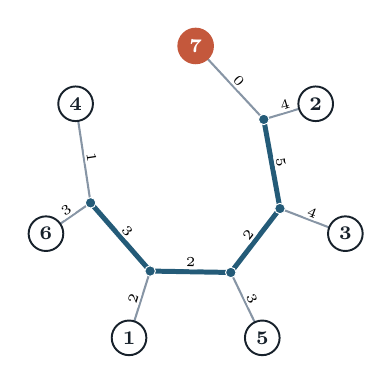
\begin{tikzpicture}[x=1cm,y=1cm]
\coordinate (v1) at (-0.84607,-1.75689);
\coordinate (v2) at (1.52457,1.21581);
\coordinate (v3) at (1.90111,-0.43392);
\coordinate (v4) at (-1.52457,1.21581);
\coordinate (v5) at (0.84607,-1.75689);
\coordinate (v6) at (-1.90111,-0.43392);
\coordinate (v7) at (0.00000,1.95000);
\coordinate (v8) at (0.86513,1.01711);
\coordinate (v9) at (-1.33461,-0.04223);
\coordinate (v10) at (-0.57814,-0.90859);
\coordinate (v11) at (1.07083,-0.11449);
\coordinate (v12) at (0.44625,-0.92666);
\draw[internal edge] (v8) -- node[edge label,pos=0.50] {$5$} (v11);
\draw[internal edge] (v9) -- node[edge label,pos=0.50] {$3$} (v10);
\draw[internal edge] (v10) -- node[edge label,pos=0.50] {$2$} (v12);
\draw[internal edge] (v11) -- node[edge label,pos=0.50] {$2$} (v12);
\draw[pendant edge] (v1) -- node[edge label,pos=0.55] {$2$} (v10);
\draw[pendant edge] (v2) -- node[edge label,pos=0.55] {$4$} (v8);
\draw[pendant edge] (v3) -- node[edge label,pos=0.55] {$4$} (v11);
\draw[pendant edge] (v4) -- node[edge label,pos=0.55] {$1$} (v9);
\draw[pendant edge] (v5) -- node[edge label,pos=0.55] {$3$} (v12);
\draw[pendant edge] (v6) -- node[edge label,pos=0.55] {$3$} (v9);
\draw[pendant edge] (v7) -- node[edge label,pos=0.55] {$0$} (v8);
\node[internal vertex] at (v8) {};
\node[internal vertex] at (v9) {};
\node[internal vertex] at (v10) {};
\node[internal vertex] at (v11) {};
\node[internal vertex] at (v12) {};
\node[leaf] at (v1) {1};
\node[leaf] at (v2) {2};
\node[leaf] at (v3) {3};
\node[leaf] at (v4) {4};
\node[leaf] at (v5) {5};
\node[leaf] at (v6) {6};
\node[special leaf] at (v7) {7};
\end{tikzpicture}
\end{minipage}
\par
\clearpage

\begin{tikzpicture}
\node[rounded corners=2pt,fill=paperblue,inner xsep=5mm,inner ysep=2mm,text width=.94\textwidth] {\Large\bfseries Orbit 2\hfill\normalsize 24 triangles};
\end{tikzpicture}\par\vspace{0.5mm}
{\scriptsize\color{muted} Triangle indices: 3, 4, 9, 10, 37, 38, 84, 85, 174, 175, 176, 177, 212, 213, 214, 215, 216, 217, 226, 227, 234, 235, 250, 251}\par{\scriptsize\color{muted} Algebra: \textcolor{toricgreen}{12 toric}, \textcolor{warningamber}{0 prime non-binomial}, \textcolor{nonprimered}{12 non-prime}.}\par\vspace{1mm}
\begin{minipage}[t][0.225\textheight][t]{0.485\textwidth}
\centering
{\normalsize\bfseries Triangle 3}\par
{\small\color{muted} Rays $\{1,\,2,\,6\}$}\par\vspace{0.3mm}
{\scriptsize \textcolor{toricgreen}{\bfseries PRIME TORIC}\color{muted}\quad $\dim/\deg=6/18$\quad GB 35/2}\par
{\scriptsize\color{bodyviolet} $f=(8,\,23,\,32,\,23,\,8)$\quad degree-one/lattice $=14/15$}\par\vspace{0.3mm}
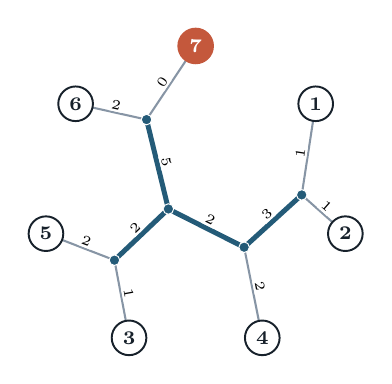
\begin{tikzpicture}[x=1cm,y=1cm]
\coordinate (v1) at (1.52457,1.21581);
\coordinate (v2) at (1.90111,-0.43392);
\coordinate (v3) at (-0.84607,-1.75689);
\coordinate (v4) at (0.84607,-1.75689);
\coordinate (v5) at (-1.90111,-0.43392);
\coordinate (v6) at (-1.52457,1.21581);
\coordinate (v7) at (0.00000,1.95000);
\coordinate (v8) at (-0.62367,1.01508);
\coordinate (v9) at (1.34709,0.05853);
\coordinate (v10) at (-1.03121,-0.77046);
\coordinate (v11) at (0.61558,-0.60631);
\coordinate (v12) at (-0.34643,-0.12056);
\draw[internal edge] (v8) -- node[edge label,pos=0.50] {$5$} (v12);
\draw[internal edge] (v9) -- node[edge label,pos=0.50] {$3$} (v11);
\draw[internal edge] (v10) -- node[edge label,pos=0.50] {$2$} (v12);
\draw[internal edge] (v11) -- node[edge label,pos=0.50] {$2$} (v12);
\draw[pendant edge] (v1) -- node[edge label,pos=0.55] {$1$} (v9);
\draw[pendant edge] (v2) -- node[edge label,pos=0.55] {$1$} (v9);
\draw[pendant edge] (v3) -- node[edge label,pos=0.55] {$1$} (v10);
\draw[pendant edge] (v4) -- node[edge label,pos=0.55] {$2$} (v11);
\draw[pendant edge] (v5) -- node[edge label,pos=0.55] {$2$} (v10);
\draw[pendant edge] (v6) -- node[edge label,pos=0.55] {$2$} (v8);
\draw[pendant edge] (v7) -- node[edge label,pos=0.55] {$0$} (v8);
\node[internal vertex] at (v8) {};
\node[internal vertex] at (v9) {};
\node[internal vertex] at (v10) {};
\node[internal vertex] at (v11) {};
\node[internal vertex] at (v12) {};
\node[leaf] at (v1) {1};
\node[leaf] at (v2) {2};
\node[leaf] at (v3) {3};
\node[leaf] at (v4) {4};
\node[leaf] at (v5) {5};
\node[leaf] at (v6) {6};
\node[special leaf] at (v7) {7};
\end{tikzpicture}
\end{minipage}
\hfill
\begin{minipage}[t][0.225\textheight][t]{0.485\textwidth}
\centering
{\normalsize\bfseries Triangle 4}\par
{\small\color{muted} Rays $\{2,\,4,\,7\}$}\par\vspace{0.3mm}
{\scriptsize \textcolor{toricgreen}{\bfseries PRIME TORIC}\color{muted}\quad $\dim/\deg=6/18$\quad GB 37/2}\par
{\scriptsize\color{bodyviolet} $f=(8,\,23,\,32,\,23,\,8)$\quad degree-one/lattice $=14/15$}\par\vspace{0.3mm}
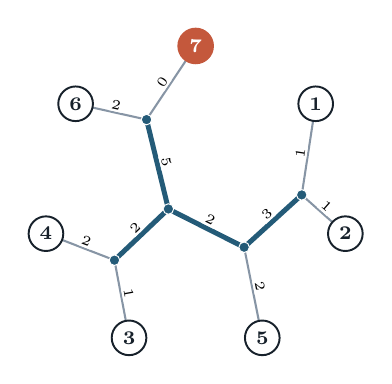
\begin{tikzpicture}[x=1cm,y=1cm]
\coordinate (v1) at (1.52457,1.21581);
\coordinate (v2) at (1.90111,-0.43392);
\coordinate (v3) at (-0.84607,-1.75689);
\coordinate (v4) at (-1.90111,-0.43392);
\coordinate (v5) at (0.84607,-1.75689);
\coordinate (v6) at (-1.52457,1.21581);
\coordinate (v7) at (0.00000,1.95000);
\coordinate (v8) at (-0.62367,1.01508);
\coordinate (v9) at (1.34709,0.05853);
\coordinate (v10) at (-1.03121,-0.77046);
\coordinate (v11) at (0.61558,-0.60631);
\coordinate (v12) at (-0.34643,-0.12056);
\draw[internal edge] (v8) -- node[edge label,pos=0.50] {$5$} (v12);
\draw[internal edge] (v9) -- node[edge label,pos=0.50] {$3$} (v11);
\draw[internal edge] (v10) -- node[edge label,pos=0.50] {$2$} (v12);
\draw[internal edge] (v11) -- node[edge label,pos=0.50] {$2$} (v12);
\draw[pendant edge] (v1) -- node[edge label,pos=0.55] {$1$} (v9);
\draw[pendant edge] (v2) -- node[edge label,pos=0.55] {$1$} (v9);
\draw[pendant edge] (v3) -- node[edge label,pos=0.55] {$1$} (v10);
\draw[pendant edge] (v4) -- node[edge label,pos=0.55] {$2$} (v10);
\draw[pendant edge] (v5) -- node[edge label,pos=0.55] {$2$} (v11);
\draw[pendant edge] (v6) -- node[edge label,pos=0.55] {$2$} (v8);
\draw[pendant edge] (v7) -- node[edge label,pos=0.55] {$0$} (v8);
\node[internal vertex] at (v8) {};
\node[internal vertex] at (v9) {};
\node[internal vertex] at (v10) {};
\node[internal vertex] at (v11) {};
\node[internal vertex] at (v12) {};
\node[leaf] at (v1) {1};
\node[leaf] at (v2) {2};
\node[leaf] at (v3) {3};
\node[leaf] at (v4) {4};
\node[leaf] at (v5) {5};
\node[leaf] at (v6) {6};
\node[special leaf] at (v7) {7};
\end{tikzpicture}
\end{minipage}
\par
\begin{minipage}[t][0.225\textheight][t]{0.485\textwidth}
\centering
{\normalsize\bfseries Triangle 9}\par
{\small\color{muted} Rays $\{1,\,3,\,11\}$}\par\vspace{0.3mm}
{\scriptsize \textcolor{nonprimered}{\bfseries NON-PRIME}\color{muted}\quad $\dim/\deg=6/18$\quad GB 35/2}\par
\vspace{1.9mm}
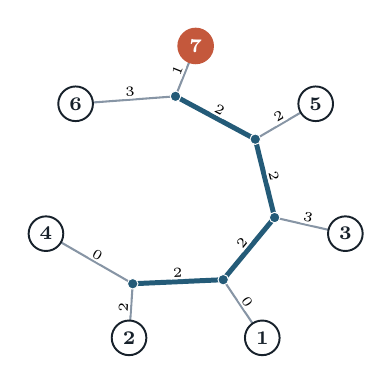
\begin{tikzpicture}[x=1cm,y=1cm]
\coordinate (v1) at (0.84607,-1.75689);
\coordinate (v2) at (-0.84607,-1.75689);
\coordinate (v3) at (1.90111,-0.43392);
\coordinate (v4) at (-1.90111,-0.43392);
\coordinate (v5) at (1.52457,1.21581);
\coordinate (v6) at (-1.52457,1.21581);
\coordinate (v7) at (0.00000,1.95000);
\coordinate (v8) at (-0.79909,-1.06977);
\coordinate (v9) at (0.34990,-1.01851);
\coordinate (v10) at (1.00273,-0.22887);
\coordinate (v11) at (0.75716,0.76583);
\coordinate (v12) at (-0.25580,1.31054);
\draw[internal edge] (v8) -- node[edge label,pos=0.50] {$2$} (v9);
\draw[internal edge] (v9) -- node[edge label,pos=0.50] {$2$} (v10);
\draw[internal edge] (v10) -- node[edge label,pos=0.50] {$2$} (v11);
\draw[internal edge] (v11) -- node[edge label,pos=0.50] {$2$} (v12);
\draw[pendant edge] (v1) -- node[edge label,pos=0.55] {$0$} (v9);
\draw[pendant edge] (v2) -- node[edge label,pos=0.55] {$2$} (v8);
\draw[pendant edge] (v3) -- node[edge label,pos=0.55] {$3$} (v10);
\draw[pendant edge] (v4) -- node[edge label,pos=0.55] {$0$} (v8);
\draw[pendant edge] (v5) -- node[edge label,pos=0.55] {$2$} (v11);
\draw[pendant edge] (v6) -- node[edge label,pos=0.55] {$3$} (v12);
\draw[pendant edge] (v7) -- node[edge label,pos=0.55] {$1$} (v12);
\node[internal vertex] at (v8) {};
\node[internal vertex] at (v9) {};
\node[internal vertex] at (v10) {};
\node[internal vertex] at (v11) {};
\node[internal vertex] at (v12) {};
\node[leaf] at (v1) {1};
\node[leaf] at (v2) {2};
\node[leaf] at (v3) {3};
\node[leaf] at (v4) {4};
\node[leaf] at (v5) {5};
\node[leaf] at (v6) {6};
\node[special leaf] at (v7) {7};
\end{tikzpicture}
\end{minipage}
\hfill
\begin{minipage}[t][0.225\textheight][t]{0.485\textwidth}
\centering
{\normalsize\bfseries Triangle 10}\par
{\small\color{muted} Rays $\{4,\,5,\,12\}$}\par\vspace{0.3mm}
{\scriptsize \textcolor{nonprimered}{\bfseries NON-PRIME}\color{muted}\quad $\dim/\deg=6/18$\quad GB 35/2}\par
\vspace{1.9mm}
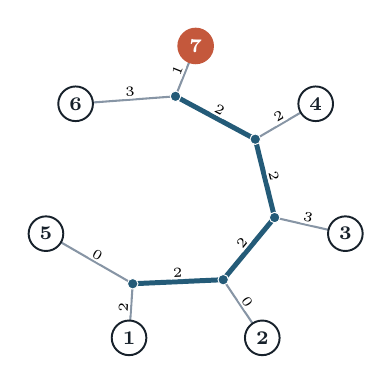
\begin{tikzpicture}[x=1cm,y=1cm]
\coordinate (v1) at (-0.84607,-1.75689);
\coordinate (v2) at (0.84607,-1.75689);
\coordinate (v3) at (1.90111,-0.43392);
\coordinate (v4) at (1.52457,1.21581);
\coordinate (v5) at (-1.90111,-0.43392);
\coordinate (v6) at (-1.52457,1.21581);
\coordinate (v7) at (0.00000,1.95000);
\coordinate (v8) at (-0.79909,-1.06977);
\coordinate (v9) at (0.34990,-1.01851);
\coordinate (v10) at (1.00273,-0.22887);
\coordinate (v11) at (0.75716,0.76583);
\coordinate (v12) at (-0.25580,1.31054);
\draw[internal edge] (v8) -- node[edge label,pos=0.50] {$2$} (v9);
\draw[internal edge] (v9) -- node[edge label,pos=0.50] {$2$} (v10);
\draw[internal edge] (v10) -- node[edge label,pos=0.50] {$2$} (v11);
\draw[internal edge] (v11) -- node[edge label,pos=0.50] {$2$} (v12);
\draw[pendant edge] (v1) -- node[edge label,pos=0.55] {$2$} (v8);
\draw[pendant edge] (v2) -- node[edge label,pos=0.55] {$0$} (v9);
\draw[pendant edge] (v3) -- node[edge label,pos=0.55] {$3$} (v10);
\draw[pendant edge] (v4) -- node[edge label,pos=0.55] {$2$} (v11);
\draw[pendant edge] (v5) -- node[edge label,pos=0.55] {$0$} (v8);
\draw[pendant edge] (v6) -- node[edge label,pos=0.55] {$3$} (v12);
\draw[pendant edge] (v7) -- node[edge label,pos=0.55] {$1$} (v12);
\node[internal vertex] at (v8) {};
\node[internal vertex] at (v9) {};
\node[internal vertex] at (v10) {};
\node[internal vertex] at (v11) {};
\node[internal vertex] at (v12) {};
\node[leaf] at (v1) {1};
\node[leaf] at (v2) {2};
\node[leaf] at (v3) {3};
\node[leaf] at (v4) {4};
\node[leaf] at (v5) {5};
\node[leaf] at (v6) {6};
\node[special leaf] at (v7) {7};
\end{tikzpicture}
\end{minipage}
\par
\begin{minipage}[t][0.225\textheight][t]{0.485\textwidth}
\centering
{\normalsize\bfseries Triangle 37}\par
{\small\color{muted} Rays $\{3,\,7,\,23\}$}\par\vspace{0.3mm}
{\scriptsize \textcolor{nonprimered}{\bfseries NON-PRIME}\color{muted}\quad $\dim/\deg=6/18$\quad GB 35/2}\par
\vspace{1.9mm}
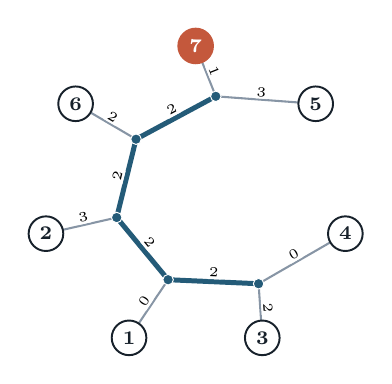
\begin{tikzpicture}[x=1cm,y=1cm]
\coordinate (v1) at (-0.84607,-1.75689);
\coordinate (v2) at (-1.90111,-0.43392);
\coordinate (v3) at (0.84607,-1.75689);
\coordinate (v4) at (1.90111,-0.43392);
\coordinate (v5) at (1.52457,1.21581);
\coordinate (v6) at (-1.52457,1.21581);
\coordinate (v7) at (0.00000,1.95000);
\coordinate (v8) at (0.79909,-1.06977);
\coordinate (v9) at (-0.34990,-1.01851);
\coordinate (v10) at (-1.00273,-0.22887);
\coordinate (v11) at (0.25580,1.31054);
\coordinate (v12) at (-0.75716,0.76583);
\draw[internal edge] (v8) -- node[edge label,pos=0.50] {$2$} (v9);
\draw[internal edge] (v9) -- node[edge label,pos=0.50] {$2$} (v10);
\draw[internal edge] (v10) -- node[edge label,pos=0.50] {$2$} (v12);
\draw[internal edge] (v11) -- node[edge label,pos=0.50] {$2$} (v12);
\draw[pendant edge] (v1) -- node[edge label,pos=0.55] {$0$} (v9);
\draw[pendant edge] (v2) -- node[edge label,pos=0.55] {$3$} (v10);
\draw[pendant edge] (v3) -- node[edge label,pos=0.55] {$2$} (v8);
\draw[pendant edge] (v4) -- node[edge label,pos=0.55] {$0$} (v8);
\draw[pendant edge] (v5) -- node[edge label,pos=0.55] {$3$} (v11);
\draw[pendant edge] (v6) -- node[edge label,pos=0.55] {$2$} (v12);
\draw[pendant edge] (v7) -- node[edge label,pos=0.55] {$1$} (v11);
\node[internal vertex] at (v8) {};
\node[internal vertex] at (v9) {};
\node[internal vertex] at (v10) {};
\node[internal vertex] at (v11) {};
\node[internal vertex] at (v12) {};
\node[leaf] at (v1) {1};
\node[leaf] at (v2) {2};
\node[leaf] at (v3) {3};
\node[leaf] at (v4) {4};
\node[leaf] at (v5) {5};
\node[leaf] at (v6) {6};
\node[special leaf] at (v7) {7};
\end{tikzpicture}
\end{minipage}
\hfill
\begin{minipage}[t][0.225\textheight][t]{0.485\textwidth}
\centering
{\normalsize\bfseries Triangle 38}\par
{\small\color{muted} Rays $\{5,\,6,\,24\}$}\par\vspace{0.3mm}
{\scriptsize \textcolor{nonprimered}{\bfseries NON-PRIME}\color{muted}\quad $\dim/\deg=6/18$\quad GB 36/2}\par
\vspace{1.9mm}
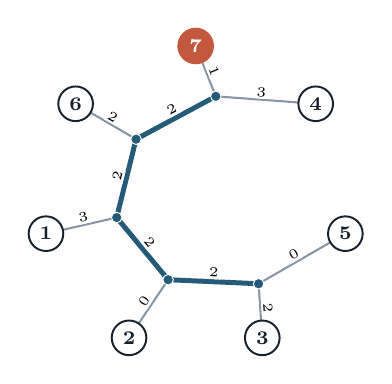
\begin{tikzpicture}[x=1cm,y=1cm]
\coordinate (v1) at (-1.90111,-0.43392);
\coordinate (v2) at (-0.84607,-1.75689);
\coordinate (v3) at (0.84607,-1.75689);
\coordinate (v4) at (1.52457,1.21581);
\coordinate (v5) at (1.90111,-0.43392);
\coordinate (v6) at (-1.52457,1.21581);
\coordinate (v7) at (0.00000,1.95000);
\coordinate (v8) at (0.79909,-1.06977);
\coordinate (v9) at (-0.34990,-1.01851);
\coordinate (v10) at (-1.00273,-0.22887);
\coordinate (v11) at (0.25580,1.31054);
\coordinate (v12) at (-0.75716,0.76583);
\draw[internal edge] (v8) -- node[edge label,pos=0.50] {$2$} (v9);
\draw[internal edge] (v9) -- node[edge label,pos=0.50] {$2$} (v10);
\draw[internal edge] (v10) -- node[edge label,pos=0.50] {$2$} (v12);
\draw[internal edge] (v11) -- node[edge label,pos=0.50] {$2$} (v12);
\draw[pendant edge] (v1) -- node[edge label,pos=0.55] {$3$} (v10);
\draw[pendant edge] (v2) -- node[edge label,pos=0.55] {$0$} (v9);
\draw[pendant edge] (v3) -- node[edge label,pos=0.55] {$2$} (v8);
\draw[pendant edge] (v4) -- node[edge label,pos=0.55] {$3$} (v11);
\draw[pendant edge] (v5) -- node[edge label,pos=0.55] {$0$} (v8);
\draw[pendant edge] (v6) -- node[edge label,pos=0.55] {$2$} (v12);
\draw[pendant edge] (v7) -- node[edge label,pos=0.55] {$1$} (v11);
\node[internal vertex] at (v8) {};
\node[internal vertex] at (v9) {};
\node[internal vertex] at (v10) {};
\node[internal vertex] at (v11) {};
\node[internal vertex] at (v12) {};
\node[leaf] at (v1) {1};
\node[leaf] at (v2) {2};
\node[leaf] at (v3) {3};
\node[leaf] at (v4) {4};
\node[leaf] at (v5) {5};
\node[leaf] at (v6) {6};
\node[special leaf] at (v7) {7};
\end{tikzpicture}
\end{minipage}
\par
\begin{minipage}[t][0.225\textheight][t]{0.485\textwidth}
\centering
{\normalsize\bfseries Triangle 84}\par
{\small\color{muted} Rays $\{7,\,16,\,38\}$}\par\vspace{0.3mm}
{\scriptsize \textcolor{nonprimered}{\bfseries NON-PRIME}\color{muted}\quad $\dim/\deg=6/18$\quad GB 42/2}\par
\vspace{1.9mm}
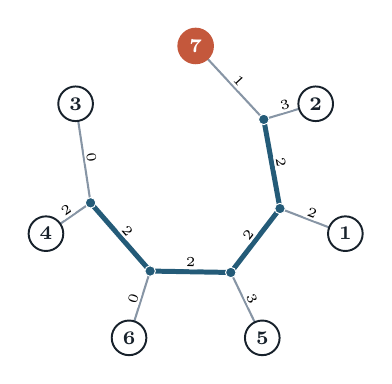
\begin{tikzpicture}[x=1cm,y=1cm]
\coordinate (v1) at (1.90111,-0.43392);
\coordinate (v2) at (1.52457,1.21581);
\coordinate (v3) at (-1.52457,1.21581);
\coordinate (v4) at (-1.90111,-0.43392);
\coordinate (v5) at (0.84607,-1.75689);
\coordinate (v6) at (-0.84607,-1.75689);
\coordinate (v7) at (0.00000,1.95000);
\coordinate (v8) at (0.86513,1.01711);
\coordinate (v9) at (1.07083,-0.11449);
\coordinate (v10) at (-1.33461,-0.04223);
\coordinate (v11) at (0.44625,-0.92666);
\coordinate (v12) at (-0.57814,-0.90859);
\draw[internal edge] (v8) -- node[edge label,pos=0.50] {$2$} (v9);
\draw[internal edge] (v9) -- node[edge label,pos=0.50] {$2$} (v11);
\draw[internal edge] (v10) -- node[edge label,pos=0.50] {$2$} (v12);
\draw[internal edge] (v11) -- node[edge label,pos=0.50] {$2$} (v12);
\draw[pendant edge] (v1) -- node[edge label,pos=0.55] {$2$} (v9);
\draw[pendant edge] (v2) -- node[edge label,pos=0.55] {$3$} (v8);
\draw[pendant edge] (v3) -- node[edge label,pos=0.55] {$0$} (v10);
\draw[pendant edge] (v4) -- node[edge label,pos=0.55] {$2$} (v10);
\draw[pendant edge] (v5) -- node[edge label,pos=0.55] {$3$} (v11);
\draw[pendant edge] (v6) -- node[edge label,pos=0.55] {$0$} (v12);
\draw[pendant edge] (v7) -- node[edge label,pos=0.55] {$1$} (v8);
\node[internal vertex] at (v8) {};
\node[internal vertex] at (v9) {};
\node[internal vertex] at (v10) {};
\node[internal vertex] at (v11) {};
\node[internal vertex] at (v12) {};
\node[leaf] at (v1) {1};
\node[leaf] at (v2) {2};
\node[leaf] at (v3) {3};
\node[leaf] at (v4) {4};
\node[leaf] at (v5) {5};
\node[leaf] at (v6) {6};
\node[special leaf] at (v7) {7};
\end{tikzpicture}
\end{minipage}
\hfill
\begin{minipage}[t][0.225\textheight][t]{0.485\textwidth}
\centering
{\normalsize\bfseries Triangle 85}\par
{\small\color{muted} Rays $\{6,\,16,\,39\}$}\par\vspace{0.3mm}
{\scriptsize \textcolor{nonprimered}{\bfseries NON-PRIME}\color{muted}\quad $\dim/\deg=6/18$\quad GB 44/2}\par
\vspace{1.9mm}
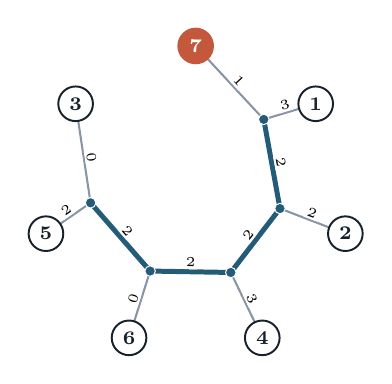
\begin{tikzpicture}[x=1cm,y=1cm]
\coordinate (v1) at (1.52457,1.21581);
\coordinate (v2) at (1.90111,-0.43392);
\coordinate (v3) at (-1.52457,1.21581);
\coordinate (v4) at (0.84607,-1.75689);
\coordinate (v5) at (-1.90111,-0.43392);
\coordinate (v6) at (-0.84607,-1.75689);
\coordinate (v7) at (0.00000,1.95000);
\coordinate (v8) at (0.86513,1.01711);
\coordinate (v9) at (1.07083,-0.11449);
\coordinate (v10) at (-1.33461,-0.04223);
\coordinate (v11) at (0.44625,-0.92666);
\coordinate (v12) at (-0.57814,-0.90859);
\draw[internal edge] (v8) -- node[edge label,pos=0.50] {$2$} (v9);
\draw[internal edge] (v9) -- node[edge label,pos=0.50] {$2$} (v11);
\draw[internal edge] (v10) -- node[edge label,pos=0.50] {$2$} (v12);
\draw[internal edge] (v11) -- node[edge label,pos=0.50] {$2$} (v12);
\draw[pendant edge] (v1) -- node[edge label,pos=0.55] {$3$} (v8);
\draw[pendant edge] (v2) -- node[edge label,pos=0.55] {$2$} (v9);
\draw[pendant edge] (v3) -- node[edge label,pos=0.55] {$0$} (v10);
\draw[pendant edge] (v4) -- node[edge label,pos=0.55] {$3$} (v11);
\draw[pendant edge] (v5) -- node[edge label,pos=0.55] {$2$} (v10);
\draw[pendant edge] (v6) -- node[edge label,pos=0.55] {$0$} (v12);
\draw[pendant edge] (v7) -- node[edge label,pos=0.55] {$1$} (v8);
\node[internal vertex] at (v8) {};
\node[internal vertex] at (v9) {};
\node[internal vertex] at (v10) {};
\node[internal vertex] at (v11) {};
\node[internal vertex] at (v12) {};
\node[leaf] at (v1) {1};
\node[leaf] at (v2) {2};
\node[leaf] at (v3) {3};
\node[leaf] at (v4) {4};
\node[leaf] at (v5) {5};
\node[leaf] at (v6) {6};
\node[special leaf] at (v7) {7};
\end{tikzpicture}
\end{minipage}
\par
\clearpage

\begin{tikzpicture}
\node[rounded corners=2pt,fill=paperblue,inner xsep=5mm,inner ysep=2mm,text width=.94\textwidth] {\Large\bfseries Orbit 2 (continued)\hfill\normalsize 24 triangles};
\end{tikzpicture}\par\vspace{0.5mm}
{\scriptsize\color{muted} Triangle indices: 3, 4, 9, 10, 37, 38, 84, 85, 174, 175, 176, 177, 212, 213, 214, 215, 216, 217, 226, 227, 234, 235, 250, 251}\par{\scriptsize\color{muted} Algebra: \textcolor{toricgreen}{12 toric}, \textcolor{warningamber}{0 prime non-binomial}, \textcolor{nonprimered}{12 non-prime}.}\par\vspace{1mm}
\begin{minipage}[t][0.225\textheight][t]{0.485\textwidth}
\centering
{\normalsize\bfseries Triangle 174}\par
{\small\color{muted} Rays $\{23,\,25,\,40\}$}\par\vspace{0.3mm}
{\scriptsize \textcolor{toricgreen}{\bfseries PRIME TORIC}\color{muted}\quad $\dim/\deg=6/18$\quad GB 36/2}\par
{\scriptsize\color{bodyviolet} $f=(8,\,23,\,32,\,23,\,8)$\quad degree-one/lattice $=14/15$}\par\vspace{0.3mm}
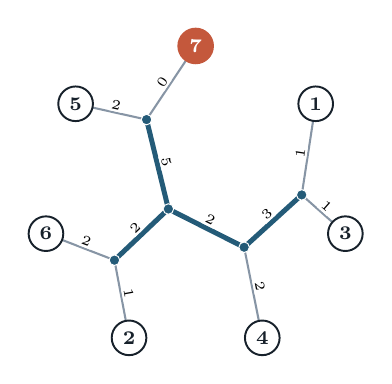
\begin{tikzpicture}[x=1cm,y=1cm]
\coordinate (v1) at (1.52457,1.21581);
\coordinate (v2) at (-0.84607,-1.75689);
\coordinate (v3) at (1.90111,-0.43392);
\coordinate (v4) at (0.84607,-1.75689);
\coordinate (v5) at (-1.52457,1.21581);
\coordinate (v6) at (-1.90111,-0.43392);
\coordinate (v7) at (0.00000,1.95000);
\coordinate (v8) at (-0.62367,1.01508);
\coordinate (v9) at (1.34709,0.05853);
\coordinate (v10) at (-1.03121,-0.77046);
\coordinate (v11) at (0.61558,-0.60631);
\coordinate (v12) at (-0.34643,-0.12056);
\draw[internal edge] (v8) -- node[edge label,pos=0.50] {$5$} (v12);
\draw[internal edge] (v9) -- node[edge label,pos=0.50] {$3$} (v11);
\draw[internal edge] (v10) -- node[edge label,pos=0.50] {$2$} (v12);
\draw[internal edge] (v11) -- node[edge label,pos=0.50] {$2$} (v12);
\draw[pendant edge] (v1) -- node[edge label,pos=0.55] {$1$} (v9);
\draw[pendant edge] (v2) -- node[edge label,pos=0.55] {$1$} (v10);
\draw[pendant edge] (v3) -- node[edge label,pos=0.55] {$1$} (v9);
\draw[pendant edge] (v4) -- node[edge label,pos=0.55] {$2$} (v11);
\draw[pendant edge] (v5) -- node[edge label,pos=0.55] {$2$} (v8);
\draw[pendant edge] (v6) -- node[edge label,pos=0.55] {$2$} (v10);
\draw[pendant edge] (v7) -- node[edge label,pos=0.55] {$0$} (v8);
\node[internal vertex] at (v8) {};
\node[internal vertex] at (v9) {};
\node[internal vertex] at (v10) {};
\node[internal vertex] at (v11) {};
\node[internal vertex] at (v12) {};
\node[leaf] at (v1) {1};
\node[leaf] at (v2) {2};
\node[leaf] at (v3) {3};
\node[leaf] at (v4) {4};
\node[leaf] at (v5) {5};
\node[leaf] at (v6) {6};
\node[special leaf] at (v7) {7};
\end{tikzpicture}
\end{minipage}
\hfill
\begin{minipage}[t][0.225\textheight][t]{0.485\textwidth}
\centering
{\normalsize\bfseries Triangle 175}\par
{\small\color{muted} Rays $\{24,\,26,\,41\}$}\par\vspace{0.3mm}
{\scriptsize \textcolor{toricgreen}{\bfseries PRIME TORIC}\color{muted}\quad $\dim/\deg=6/18$\quad GB 35/2}\par
{\scriptsize\color{bodyviolet} $f=(8,\,23,\,32,\,23,\,8)$\quad degree-one/lattice $=14/15$}\par\vspace{0.3mm}
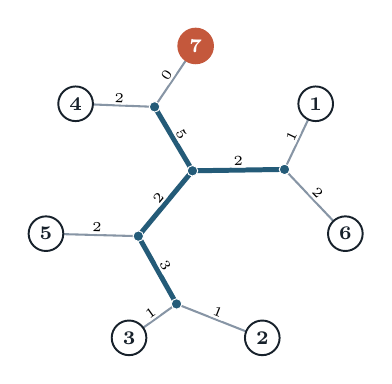
\begin{tikzpicture}[x=1cm,y=1cm]
\coordinate (v1) at (1.52457,1.21581);
\coordinate (v2) at (0.84607,-1.75689);
\coordinate (v3) at (-0.84607,-1.75689);
\coordinate (v4) at (-1.52457,1.21581);
\coordinate (v5) at (-1.90111,-0.43392);
\coordinate (v6) at (1.90111,-0.43392);
\coordinate (v7) at (0.00000,1.95000);
\coordinate (v8) at (-0.52167,1.17679);
\coordinate (v9) at (-0.24269,-1.32633);
\coordinate (v10) at (1.12841,0.38215);
\coordinate (v11) at (-0.72808,-0.46523);
\coordinate (v12) at (-0.04045,0.36457);
\draw[internal edge] (v8) -- node[edge label,pos=0.50] {$5$} (v12);
\draw[internal edge] (v9) -- node[edge label,pos=0.50] {$3$} (v11);
\draw[internal edge] (v10) -- node[edge label,pos=0.50] {$2$} (v12);
\draw[internal edge] (v11) -- node[edge label,pos=0.50] {$2$} (v12);
\draw[pendant edge] (v1) -- node[edge label,pos=0.55] {$1$} (v10);
\draw[pendant edge] (v2) -- node[edge label,pos=0.55] {$1$} (v9);
\draw[pendant edge] (v3) -- node[edge label,pos=0.55] {$1$} (v9);
\draw[pendant edge] (v4) -- node[edge label,pos=0.55] {$2$} (v8);
\draw[pendant edge] (v5) -- node[edge label,pos=0.55] {$2$} (v11);
\draw[pendant edge] (v6) -- node[edge label,pos=0.55] {$2$} (v10);
\draw[pendant edge] (v7) -- node[edge label,pos=0.55] {$0$} (v8);
\node[internal vertex] at (v8) {};
\node[internal vertex] at (v9) {};
\node[internal vertex] at (v10) {};
\node[internal vertex] at (v11) {};
\node[internal vertex] at (v12) {};
\node[leaf] at (v1) {1};
\node[leaf] at (v2) {2};
\node[leaf] at (v3) {3};
\node[leaf] at (v4) {4};
\node[leaf] at (v5) {5};
\node[leaf] at (v6) {6};
\node[special leaf] at (v7) {7};
\end{tikzpicture}
\end{minipage}
\par
\begin{minipage}[t][0.225\textheight][t]{0.485\textwidth}
\centering
{\normalsize\bfseries Triangle 176}\par
{\small\color{muted} Rays $\{28,\,41,\,42\}$}\par\vspace{0.3mm}
{\scriptsize \textcolor{toricgreen}{\bfseries PRIME TORIC}\color{muted}\quad $\dim/\deg=6/18$\quad GB 42/2}\par
{\scriptsize\color{bodyviolet} $f=(8,\,23,\,32,\,23,\,8)$\quad degree-one/lattice $=14/15$}\par\vspace{0.3mm}
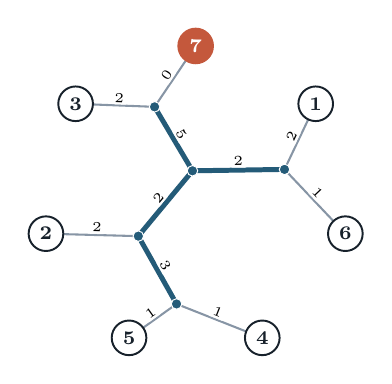
\begin{tikzpicture}[x=1cm,y=1cm]
\coordinate (v1) at (1.52457,1.21581);
\coordinate (v2) at (-1.90111,-0.43392);
\coordinate (v3) at (-1.52457,1.21581);
\coordinate (v4) at (0.84607,-1.75689);
\coordinate (v5) at (-0.84607,-1.75689);
\coordinate (v6) at (1.90111,-0.43392);
\coordinate (v7) at (0.00000,1.95000);
\coordinate (v8) at (-0.52167,1.17679);
\coordinate (v9) at (-0.24269,-1.32633);
\coordinate (v10) at (1.12841,0.38215);
\coordinate (v11) at (-0.72808,-0.46523);
\coordinate (v12) at (-0.04045,0.36457);
\draw[internal edge] (v8) -- node[edge label,pos=0.50] {$5$} (v12);
\draw[internal edge] (v9) -- node[edge label,pos=0.50] {$3$} (v11);
\draw[internal edge] (v10) -- node[edge label,pos=0.50] {$2$} (v12);
\draw[internal edge] (v11) -- node[edge label,pos=0.50] {$2$} (v12);
\draw[pendant edge] (v1) -- node[edge label,pos=0.55] {$2$} (v10);
\draw[pendant edge] (v2) -- node[edge label,pos=0.55] {$2$} (v11);
\draw[pendant edge] (v3) -- node[edge label,pos=0.55] {$2$} (v8);
\draw[pendant edge] (v4) -- node[edge label,pos=0.55] {$1$} (v9);
\draw[pendant edge] (v5) -- node[edge label,pos=0.55] {$1$} (v9);
\draw[pendant edge] (v6) -- node[edge label,pos=0.55] {$1$} (v10);
\draw[pendant edge] (v7) -- node[edge label,pos=0.55] {$0$} (v8);
\node[internal vertex] at (v8) {};
\node[internal vertex] at (v9) {};
\node[internal vertex] at (v10) {};
\node[internal vertex] at (v11) {};
\node[internal vertex] at (v12) {};
\node[leaf] at (v1) {1};
\node[leaf] at (v2) {2};
\node[leaf] at (v3) {3};
\node[leaf] at (v4) {4};
\node[leaf] at (v5) {5};
\node[leaf] at (v6) {6};
\node[special leaf] at (v7) {7};
\end{tikzpicture}
\end{minipage}
\hfill
\begin{minipage}[t][0.225\textheight][t]{0.485\textwidth}
\centering
{\normalsize\bfseries Triangle 177}\par
{\small\color{muted} Rays $\{28,\,40,\,43\}$}\par\vspace{0.3mm}
{\scriptsize \textcolor{toricgreen}{\bfseries PRIME TORIC}\color{muted}\quad $\dim/\deg=6/18$\quad GB 47/2}\par
{\scriptsize\color{bodyviolet} $f=(8,\,23,\,32,\,23,\,8)$\quad degree-one/lattice $=14/15$}\par\vspace{0.3mm}
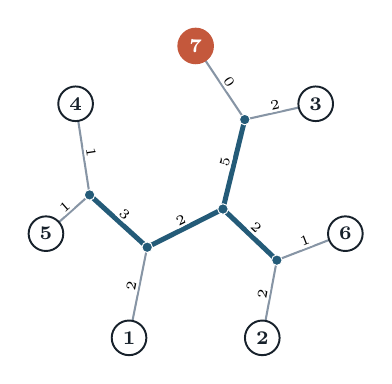
\begin{tikzpicture}[x=1cm,y=1cm]
\coordinate (v1) at (-0.84607,-1.75689);
\coordinate (v2) at (0.84607,-1.75689);
\coordinate (v3) at (1.52457,1.21581);
\coordinate (v4) at (-1.52457,1.21581);
\coordinate (v5) at (-1.90111,-0.43392);
\coordinate (v6) at (1.90111,-0.43392);
\coordinate (v7) at (0.00000,1.95000);
\coordinate (v8) at (0.62367,1.01508);
\coordinate (v9) at (-1.34709,0.05853);
\coordinate (v10) at (-0.61558,-0.60631);
\coordinate (v11) at (1.03121,-0.77046);
\coordinate (v12) at (0.34643,-0.12056);
\draw[internal edge] (v8) -- node[edge label,pos=0.50] {$5$} (v12);
\draw[internal edge] (v9) -- node[edge label,pos=0.50] {$3$} (v10);
\draw[internal edge] (v10) -- node[edge label,pos=0.50] {$2$} (v12);
\draw[internal edge] (v11) -- node[edge label,pos=0.50] {$2$} (v12);
\draw[pendant edge] (v1) -- node[edge label,pos=0.55] {$2$} (v10);
\draw[pendant edge] (v2) -- node[edge label,pos=0.55] {$2$} (v11);
\draw[pendant edge] (v3) -- node[edge label,pos=0.55] {$2$} (v8);
\draw[pendant edge] (v4) -- node[edge label,pos=0.55] {$1$} (v9);
\draw[pendant edge] (v5) -- node[edge label,pos=0.55] {$1$} (v9);
\draw[pendant edge] (v6) -- node[edge label,pos=0.55] {$1$} (v11);
\draw[pendant edge] (v7) -- node[edge label,pos=0.55] {$0$} (v8);
\node[internal vertex] at (v8) {};
\node[internal vertex] at (v9) {};
\node[internal vertex] at (v10) {};
\node[internal vertex] at (v11) {};
\node[internal vertex] at (v12) {};
\node[leaf] at (v1) {1};
\node[leaf] at (v2) {2};
\node[leaf] at (v3) {3};
\node[leaf] at (v4) {4};
\node[leaf] at (v5) {5};
\node[leaf] at (v6) {6};
\node[special leaf] at (v7) {7};
\end{tikzpicture}
\end{minipage}
\par
\begin{minipage}[t][0.225\textheight][t]{0.485\textwidth}
\centering
{\normalsize\bfseries Triangle 212}\par
{\small\color{muted} Rays $\{11,\,25,\,48\}$}\par\vspace{0.3mm}
{\scriptsize \textcolor{toricgreen}{\bfseries PRIME TORIC}\color{muted}\quad $\dim/\deg=6/18$\quad GB 37/2}\par
{\scriptsize\color{bodyviolet} $f=(8,\,23,\,32,\,23,\,8)$\quad degree-one/lattice $=14/15$}\par\vspace{0.3mm}
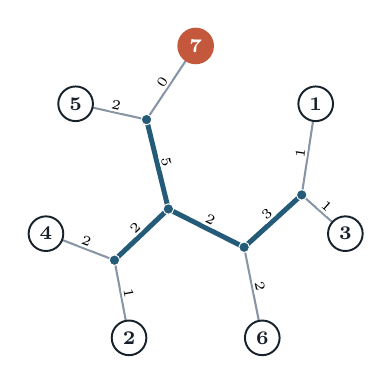
\begin{tikzpicture}[x=1cm,y=1cm]
\coordinate (v1) at (1.52457,1.21581);
\coordinate (v2) at (-0.84607,-1.75689);
\coordinate (v3) at (1.90111,-0.43392);
\coordinate (v4) at (-1.90111,-0.43392);
\coordinate (v5) at (-1.52457,1.21581);
\coordinate (v6) at (0.84607,-1.75689);
\coordinate (v7) at (0.00000,1.95000);
\coordinate (v8) at (-0.62367,1.01508);
\coordinate (v9) at (1.34709,0.05853);
\coordinate (v10) at (-1.03121,-0.77046);
\coordinate (v11) at (0.61558,-0.60631);
\coordinate (v12) at (-0.34643,-0.12056);
\draw[internal edge] (v8) -- node[edge label,pos=0.50] {$5$} (v12);
\draw[internal edge] (v9) -- node[edge label,pos=0.50] {$3$} (v11);
\draw[internal edge] (v10) -- node[edge label,pos=0.50] {$2$} (v12);
\draw[internal edge] (v11) -- node[edge label,pos=0.50] {$2$} (v12);
\draw[pendant edge] (v1) -- node[edge label,pos=0.55] {$1$} (v9);
\draw[pendant edge] (v2) -- node[edge label,pos=0.55] {$1$} (v10);
\draw[pendant edge] (v3) -- node[edge label,pos=0.55] {$1$} (v9);
\draw[pendant edge] (v4) -- node[edge label,pos=0.55] {$2$} (v10);
\draw[pendant edge] (v5) -- node[edge label,pos=0.55] {$2$} (v8);
\draw[pendant edge] (v6) -- node[edge label,pos=0.55] {$2$} (v11);
\draw[pendant edge] (v7) -- node[edge label,pos=0.55] {$0$} (v8);
\node[internal vertex] at (v8) {};
\node[internal vertex] at (v9) {};
\node[internal vertex] at (v10) {};
\node[internal vertex] at (v11) {};
\node[internal vertex] at (v12) {};
\node[leaf] at (v1) {1};
\node[leaf] at (v2) {2};
\node[leaf] at (v3) {3};
\node[leaf] at (v4) {4};
\node[leaf] at (v5) {5};
\node[leaf] at (v6) {6};
\node[special leaf] at (v7) {7};
\end{tikzpicture}
\end{minipage}
\hfill
\begin{minipage}[t][0.225\textheight][t]{0.485\textwidth}
\centering
{\normalsize\bfseries Triangle 213}\par
{\small\color{muted} Rays $\{12,\,26,\,49\}$}\par\vspace{0.3mm}
{\scriptsize \textcolor{toricgreen}{\bfseries PRIME TORIC}\color{muted}\quad $\dim/\deg=6/18$\quad GB 39/2}\par
{\scriptsize\color{bodyviolet} $f=(8,\,23,\,32,\,23,\,8)$\quad degree-one/lattice $=14/15$}\par\vspace{0.3mm}
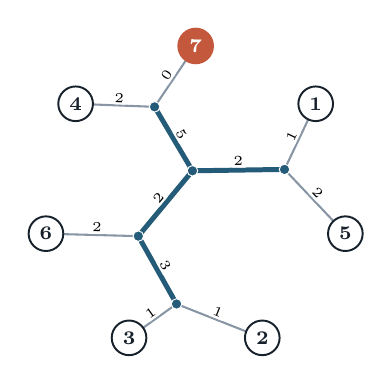
\begin{tikzpicture}[x=1cm,y=1cm]
\coordinate (v1) at (1.52457,1.21581);
\coordinate (v2) at (0.84607,-1.75689);
\coordinate (v3) at (-0.84607,-1.75689);
\coordinate (v4) at (-1.52457,1.21581);
\coordinate (v5) at (1.90111,-0.43392);
\coordinate (v6) at (-1.90111,-0.43392);
\coordinate (v7) at (0.00000,1.95000);
\coordinate (v8) at (-0.52167,1.17679);
\coordinate (v9) at (-0.24269,-1.32633);
\coordinate (v10) at (1.12841,0.38215);
\coordinate (v11) at (-0.72808,-0.46523);
\coordinate (v12) at (-0.04045,0.36457);
\draw[internal edge] (v8) -- node[edge label,pos=0.50] {$5$} (v12);
\draw[internal edge] (v9) -- node[edge label,pos=0.50] {$3$} (v11);
\draw[internal edge] (v10) -- node[edge label,pos=0.50] {$2$} (v12);
\draw[internal edge] (v11) -- node[edge label,pos=0.50] {$2$} (v12);
\draw[pendant edge] (v1) -- node[edge label,pos=0.55] {$1$} (v10);
\draw[pendant edge] (v2) -- node[edge label,pos=0.55] {$1$} (v9);
\draw[pendant edge] (v3) -- node[edge label,pos=0.55] {$1$} (v9);
\draw[pendant edge] (v4) -- node[edge label,pos=0.55] {$2$} (v8);
\draw[pendant edge] (v5) -- node[edge label,pos=0.55] {$2$} (v10);
\draw[pendant edge] (v6) -- node[edge label,pos=0.55] {$2$} (v11);
\draw[pendant edge] (v7) -- node[edge label,pos=0.55] {$0$} (v8);
\node[internal vertex] at (v8) {};
\node[internal vertex] at (v9) {};
\node[internal vertex] at (v10) {};
\node[internal vertex] at (v11) {};
\node[internal vertex] at (v12) {};
\node[leaf] at (v1) {1};
\node[leaf] at (v2) {2};
\node[leaf] at (v3) {3};
\node[leaf] at (v4) {4};
\node[leaf] at (v5) {5};
\node[leaf] at (v6) {6};
\node[special leaf] at (v7) {7};
\end{tikzpicture}
\end{minipage}
\par
\begin{minipage}[t][0.225\textheight][t]{0.485\textwidth}
\centering
{\normalsize\bfseries Triangle 214}\par
{\small\color{muted} Rays $\{12,\,32,\,38\}$}\par\vspace{0.3mm}
{\scriptsize \textcolor{toricgreen}{\bfseries PRIME TORIC}\color{muted}\quad $\dim/\deg=6/18$\quad GB 41/2}\par
{\scriptsize\color{bodyviolet} $f=(8,\,23,\,32,\,23,\,8)$\quad degree-one/lattice $=14/15$}\par\vspace{0.3mm}
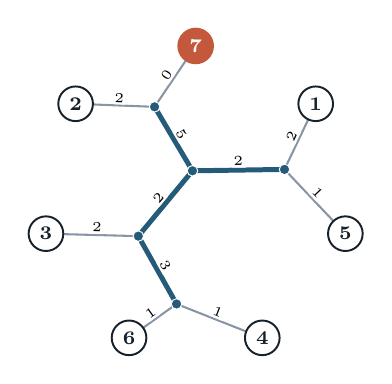
\begin{tikzpicture}[x=1cm,y=1cm]
\coordinate (v1) at (1.52457,1.21581);
\coordinate (v2) at (-1.52457,1.21581);
\coordinate (v3) at (-1.90111,-0.43392);
\coordinate (v4) at (0.84607,-1.75689);
\coordinate (v5) at (1.90111,-0.43392);
\coordinate (v6) at (-0.84607,-1.75689);
\coordinate (v7) at (0.00000,1.95000);
\coordinate (v8) at (-0.52167,1.17679);
\coordinate (v9) at (-0.24269,-1.32633);
\coordinate (v10) at (1.12841,0.38215);
\coordinate (v11) at (-0.72808,-0.46523);
\coordinate (v12) at (-0.04045,0.36457);
\draw[internal edge] (v8) -- node[edge label,pos=0.50] {$5$} (v12);
\draw[internal edge] (v9) -- node[edge label,pos=0.50] {$3$} (v11);
\draw[internal edge] (v10) -- node[edge label,pos=0.50] {$2$} (v12);
\draw[internal edge] (v11) -- node[edge label,pos=0.50] {$2$} (v12);
\draw[pendant edge] (v1) -- node[edge label,pos=0.55] {$2$} (v10);
\draw[pendant edge] (v2) -- node[edge label,pos=0.55] {$2$} (v8);
\draw[pendant edge] (v3) -- node[edge label,pos=0.55] {$2$} (v11);
\draw[pendant edge] (v4) -- node[edge label,pos=0.55] {$1$} (v9);
\draw[pendant edge] (v5) -- node[edge label,pos=0.55] {$1$} (v10);
\draw[pendant edge] (v6) -- node[edge label,pos=0.55] {$1$} (v9);
\draw[pendant edge] (v7) -- node[edge label,pos=0.55] {$0$} (v8);
\node[internal vertex] at (v8) {};
\node[internal vertex] at (v9) {};
\node[internal vertex] at (v10) {};
\node[internal vertex] at (v11) {};
\node[internal vertex] at (v12) {};
\node[leaf] at (v1) {1};
\node[leaf] at (v2) {2};
\node[leaf] at (v3) {3};
\node[leaf] at (v4) {4};
\node[leaf] at (v5) {5};
\node[leaf] at (v6) {6};
\node[special leaf] at (v7) {7};
\end{tikzpicture}
\end{minipage}
\hfill
\begin{minipage}[t][0.225\textheight][t]{0.485\textwidth}
\centering
{\normalsize\bfseries Triangle 215}\par
{\small\color{muted} Rays $\{11,\,31,\,39\}$}\par\vspace{0.3mm}
{\scriptsize \textcolor{toricgreen}{\bfseries PRIME TORIC}\color{muted}\quad $\dim/\deg=6/18$\quad GB 40/2}\par
{\scriptsize\color{bodyviolet} $f=(8,\,23,\,32,\,23,\,8)$\quad degree-one/lattice $=14/15$}\par\vspace{0.3mm}
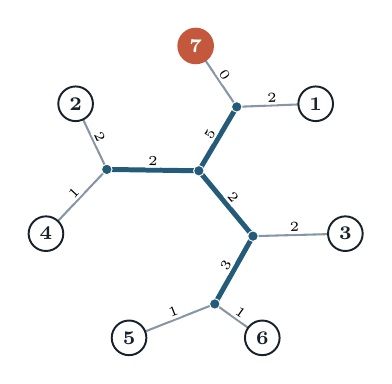
\begin{tikzpicture}[x=1cm,y=1cm]
\coordinate (v1) at (1.52457,1.21581);
\coordinate (v2) at (-1.52457,1.21581);
\coordinate (v3) at (1.90111,-0.43392);
\coordinate (v4) at (-1.90111,-0.43392);
\coordinate (v5) at (-0.84607,-1.75689);
\coordinate (v6) at (0.84607,-1.75689);
\coordinate (v7) at (0.00000,1.95000);
\coordinate (v8) at (0.52167,1.17679);
\coordinate (v9) at (0.24269,-1.32633);
\coordinate (v10) at (-1.12841,0.38215);
\coordinate (v11) at (0.72808,-0.46523);
\coordinate (v12) at (0.04045,0.36457);
\draw[internal edge] (v8) -- node[edge label,pos=0.50] {$5$} (v12);
\draw[internal edge] (v9) -- node[edge label,pos=0.50] {$3$} (v11);
\draw[internal edge] (v10) -- node[edge label,pos=0.50] {$2$} (v12);
\draw[internal edge] (v11) -- node[edge label,pos=0.50] {$2$} (v12);
\draw[pendant edge] (v1) -- node[edge label,pos=0.55] {$2$} (v8);
\draw[pendant edge] (v2) -- node[edge label,pos=0.55] {$2$} (v10);
\draw[pendant edge] (v3) -- node[edge label,pos=0.55] {$2$} (v11);
\draw[pendant edge] (v4) -- node[edge label,pos=0.55] {$1$} (v10);
\draw[pendant edge] (v5) -- node[edge label,pos=0.55] {$1$} (v9);
\draw[pendant edge] (v6) -- node[edge label,pos=0.55] {$1$} (v9);
\draw[pendant edge] (v7) -- node[edge label,pos=0.55] {$0$} (v8);
\node[internal vertex] at (v8) {};
\node[internal vertex] at (v9) {};
\node[internal vertex] at (v10) {};
\node[internal vertex] at (v11) {};
\node[internal vertex] at (v12) {};
\node[leaf] at (v1) {1};
\node[leaf] at (v2) {2};
\node[leaf] at (v3) {3};
\node[leaf] at (v4) {4};
\node[leaf] at (v5) {5};
\node[leaf] at (v6) {6};
\node[special leaf] at (v7) {7};
\end{tikzpicture}
\end{minipage}
\par
\clearpage

\begin{tikzpicture}
\node[rounded corners=2pt,fill=paperblue,inner xsep=5mm,inner ysep=2mm,text width=.94\textwidth] {\Large\bfseries Orbit 2 (continued)\hfill\normalsize 24 triangles};
\end{tikzpicture}\par\vspace{0.5mm}
{\scriptsize\color{muted} Triangle indices: 3, 4, 9, 10, 37, 38, 84, 85, 174, 175, 176, 177, 212, 213, 214, 215, 216, 217, 226, 227, 234, 235, 250, 251}\par{\scriptsize\color{muted} Algebra: \textcolor{toricgreen}{12 toric}, \textcolor{warningamber}{0 prime non-binomial}, \textcolor{nonprimered}{12 non-prime}.}\par\vspace{1mm}
\begin{minipage}[t][0.225\textheight][t]{0.485\textwidth}
\centering
{\normalsize\bfseries Triangle 216}\par
{\small\color{muted} Rays $\{11,\,42,\,46\}$}\par\vspace{0.3mm}
{\scriptsize \textcolor{nonprimered}{\bfseries NON-PRIME}\color{muted}\quad $\dim/\deg=6/18$\quad GB 37/2}\par
\vspace{1.9mm}
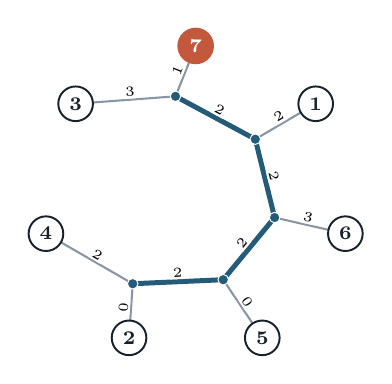
\begin{tikzpicture}[x=1cm,y=1cm]
\coordinate (v1) at (1.52457,1.21581);
\coordinate (v2) at (-0.84607,-1.75689);
\coordinate (v3) at (-1.52457,1.21581);
\coordinate (v4) at (-1.90111,-0.43392);
\coordinate (v5) at (0.84607,-1.75689);
\coordinate (v6) at (1.90111,-0.43392);
\coordinate (v7) at (0.00000,1.95000);
\coordinate (v8) at (-0.79909,-1.06977);
\coordinate (v9) at (-0.25580,1.31054);
\coordinate (v10) at (0.75716,0.76583);
\coordinate (v11) at (0.34990,-1.01851);
\coordinate (v12) at (1.00273,-0.22887);
\draw[internal edge] (v8) -- node[edge label,pos=0.50] {$2$} (v11);
\draw[internal edge] (v9) -- node[edge label,pos=0.50] {$2$} (v10);
\draw[internal edge] (v10) -- node[edge label,pos=0.50] {$2$} (v12);
\draw[internal edge] (v11) -- node[edge label,pos=0.50] {$2$} (v12);
\draw[pendant edge] (v1) -- node[edge label,pos=0.55] {$2$} (v10);
\draw[pendant edge] (v2) -- node[edge label,pos=0.55] {$0$} (v8);
\draw[pendant edge] (v3) -- node[edge label,pos=0.55] {$3$} (v9);
\draw[pendant edge] (v4) -- node[edge label,pos=0.55] {$2$} (v8);
\draw[pendant edge] (v5) -- node[edge label,pos=0.55] {$0$} (v11);
\draw[pendant edge] (v6) -- node[edge label,pos=0.55] {$3$} (v12);
\draw[pendant edge] (v7) -- node[edge label,pos=0.55] {$1$} (v9);
\node[internal vertex] at (v8) {};
\node[internal vertex] at (v9) {};
\node[internal vertex] at (v10) {};
\node[internal vertex] at (v11) {};
\node[internal vertex] at (v12) {};
\node[leaf] at (v1) {1};
\node[leaf] at (v2) {2};
\node[leaf] at (v3) {3};
\node[leaf] at (v4) {4};
\node[leaf] at (v5) {5};
\node[leaf] at (v6) {6};
\node[special leaf] at (v7) {7};
\end{tikzpicture}
\end{minipage}
\hfill
\begin{minipage}[t][0.225\textheight][t]{0.485\textwidth}
\centering
{\normalsize\bfseries Triangle 217}\par
{\small\color{muted} Rays $\{12,\,43,\,47\}$}\par\vspace{0.3mm}
{\scriptsize \textcolor{nonprimered}{\bfseries NON-PRIME}\color{muted}\quad $\dim/\deg=6/18$\quad GB 39/2}\par
\vspace{1.9mm}
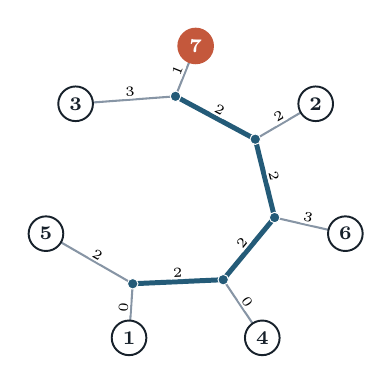
\begin{tikzpicture}[x=1cm,y=1cm]
\coordinate (v1) at (-0.84607,-1.75689);
\coordinate (v2) at (1.52457,1.21581);
\coordinate (v3) at (-1.52457,1.21581);
\coordinate (v4) at (0.84607,-1.75689);
\coordinate (v5) at (-1.90111,-0.43392);
\coordinate (v6) at (1.90111,-0.43392);
\coordinate (v7) at (0.00000,1.95000);
\coordinate (v8) at (-0.79909,-1.06977);
\coordinate (v9) at (-0.25580,1.31054);
\coordinate (v10) at (0.75716,0.76583);
\coordinate (v11) at (0.34990,-1.01851);
\coordinate (v12) at (1.00273,-0.22887);
\draw[internal edge] (v8) -- node[edge label,pos=0.50] {$2$} (v11);
\draw[internal edge] (v9) -- node[edge label,pos=0.50] {$2$} (v10);
\draw[internal edge] (v10) -- node[edge label,pos=0.50] {$2$} (v12);
\draw[internal edge] (v11) -- node[edge label,pos=0.50] {$2$} (v12);
\draw[pendant edge] (v1) -- node[edge label,pos=0.55] {$0$} (v8);
\draw[pendant edge] (v2) -- node[edge label,pos=0.55] {$2$} (v10);
\draw[pendant edge] (v3) -- node[edge label,pos=0.55] {$3$} (v9);
\draw[pendant edge] (v4) -- node[edge label,pos=0.55] {$0$} (v11);
\draw[pendant edge] (v5) -- node[edge label,pos=0.55] {$2$} (v8);
\draw[pendant edge] (v6) -- node[edge label,pos=0.55] {$3$} (v12);
\draw[pendant edge] (v7) -- node[edge label,pos=0.55] {$1$} (v9);
\node[internal vertex] at (v8) {};
\node[internal vertex] at (v9) {};
\node[internal vertex] at (v10) {};
\node[internal vertex] at (v11) {};
\node[internal vertex] at (v12) {};
\node[leaf] at (v1) {1};
\node[leaf] at (v2) {2};
\node[leaf] at (v3) {3};
\node[leaf] at (v4) {4};
\node[leaf] at (v5) {5};
\node[leaf] at (v6) {6};
\node[special leaf] at (v7) {7};
\end{tikzpicture}
\end{minipage}
\par
\begin{minipage}[t][0.225\textheight][t]{0.485\textwidth}
\centering
{\normalsize\bfseries Triangle 226}\par
{\small\color{muted} Rays $\{27,\,41,\,48\}$}\par\vspace{0.3mm}
{\scriptsize \textcolor{nonprimered}{\bfseries NON-PRIME}\color{muted}\quad $\dim/\deg=6/18$\quad GB 42/2}\par
\vspace{1.9mm}
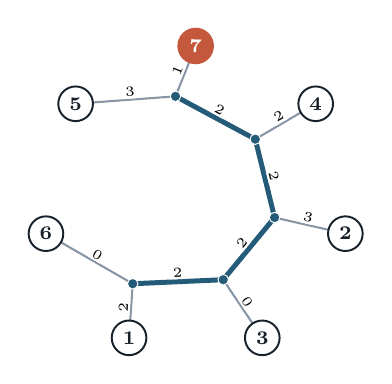
\begin{tikzpicture}[x=1cm,y=1cm]
\coordinate (v1) at (-0.84607,-1.75689);
\coordinate (v2) at (1.90111,-0.43392);
\coordinate (v3) at (0.84607,-1.75689);
\coordinate (v4) at (1.52457,1.21581);
\coordinate (v5) at (-1.52457,1.21581);
\coordinate (v6) at (-1.90111,-0.43392);
\coordinate (v7) at (0.00000,1.95000);
\coordinate (v8) at (-0.79909,-1.06977);
\coordinate (v9) at (0.34990,-1.01851);
\coordinate (v10) at (1.00273,-0.22887);
\coordinate (v11) at (0.75716,0.76583);
\coordinate (v12) at (-0.25580,1.31054);
\draw[internal edge] (v8) -- node[edge label,pos=0.50] {$2$} (v9);
\draw[internal edge] (v9) -- node[edge label,pos=0.50] {$2$} (v10);
\draw[internal edge] (v10) -- node[edge label,pos=0.50] {$2$} (v11);
\draw[internal edge] (v11) -- node[edge label,pos=0.50] {$2$} (v12);
\draw[pendant edge] (v1) -- node[edge label,pos=0.55] {$2$} (v8);
\draw[pendant edge] (v2) -- node[edge label,pos=0.55] {$3$} (v10);
\draw[pendant edge] (v3) -- node[edge label,pos=0.55] {$0$} (v9);
\draw[pendant edge] (v4) -- node[edge label,pos=0.55] {$2$} (v11);
\draw[pendant edge] (v5) -- node[edge label,pos=0.55] {$3$} (v12);
\draw[pendant edge] (v6) -- node[edge label,pos=0.55] {$0$} (v8);
\draw[pendant edge] (v7) -- node[edge label,pos=0.55] {$1$} (v12);
\node[internal vertex] at (v8) {};
\node[internal vertex] at (v9) {};
\node[internal vertex] at (v10) {};
\node[internal vertex] at (v11) {};
\node[internal vertex] at (v12) {};
\node[leaf] at (v1) {1};
\node[leaf] at (v2) {2};
\node[leaf] at (v3) {3};
\node[leaf] at (v4) {4};
\node[leaf] at (v5) {5};
\node[leaf] at (v6) {6};
\node[special leaf] at (v7) {7};
\end{tikzpicture}
\end{minipage}
\hfill
\begin{minipage}[t][0.225\textheight][t]{0.485\textwidth}
\centering
{\normalsize\bfseries Triangle 227}\par
{\small\color{muted} Rays $\{27,\,40,\,49\}$}\par\vspace{0.3mm}
{\scriptsize \textcolor{nonprimered}{\bfseries NON-PRIME}\color{muted}\quad $\dim/\deg=6/18$\quad GB 42/2}\par
\vspace{1.9mm}
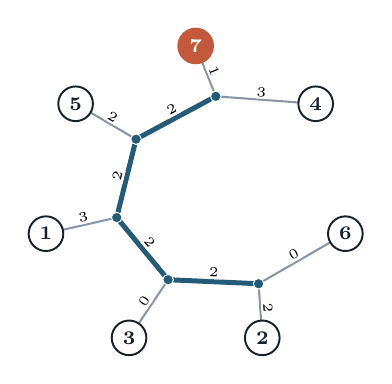
\begin{tikzpicture}[x=1cm,y=1cm]
\coordinate (v1) at (-1.90111,-0.43392);
\coordinate (v2) at (0.84607,-1.75689);
\coordinate (v3) at (-0.84607,-1.75689);
\coordinate (v4) at (1.52457,1.21581);
\coordinate (v5) at (-1.52457,1.21581);
\coordinate (v6) at (1.90111,-0.43392);
\coordinate (v7) at (0.00000,1.95000);
\coordinate (v8) at (0.79909,-1.06977);
\coordinate (v9) at (-0.34990,-1.01851);
\coordinate (v10) at (-1.00273,-0.22887);
\coordinate (v11) at (0.25580,1.31054);
\coordinate (v12) at (-0.75716,0.76583);
\draw[internal edge] (v8) -- node[edge label,pos=0.50] {$2$} (v9);
\draw[internal edge] (v9) -- node[edge label,pos=0.50] {$2$} (v10);
\draw[internal edge] (v10) -- node[edge label,pos=0.50] {$2$} (v12);
\draw[internal edge] (v11) -- node[edge label,pos=0.50] {$2$} (v12);
\draw[pendant edge] (v1) -- node[edge label,pos=0.55] {$3$} (v10);
\draw[pendant edge] (v2) -- node[edge label,pos=0.55] {$2$} (v8);
\draw[pendant edge] (v3) -- node[edge label,pos=0.55] {$0$} (v9);
\draw[pendant edge] (v4) -- node[edge label,pos=0.55] {$3$} (v11);
\draw[pendant edge] (v5) -- node[edge label,pos=0.55] {$2$} (v12);
\draw[pendant edge] (v6) -- node[edge label,pos=0.55] {$0$} (v8);
\draw[pendant edge] (v7) -- node[edge label,pos=0.55] {$1$} (v11);
\node[internal vertex] at (v8) {};
\node[internal vertex] at (v9) {};
\node[internal vertex] at (v10) {};
\node[internal vertex] at (v11) {};
\node[internal vertex] at (v12) {};
\node[leaf] at (v1) {1};
\node[leaf] at (v2) {2};
\node[leaf] at (v3) {3};
\node[leaf] at (v4) {4};
\node[leaf] at (v5) {5};
\node[leaf] at (v6) {6};
\node[special leaf] at (v7) {7};
\end{tikzpicture}
\end{minipage}
\par
\begin{minipage}[t][0.225\textheight][t]{0.485\textwidth}
\centering
{\normalsize\bfseries Triangle 234}\par
{\small\color{muted} Rays $\{6,\,32,\,50\}$}\par\vspace{0.3mm}
{\scriptsize \textcolor{toricgreen}{\bfseries PRIME TORIC}\color{muted}\quad $\dim/\deg=6/18$\quad GB 42/2}\par
{\scriptsize\color{bodyviolet} $f=(8,\,23,\,32,\,23,\,8)$\quad degree-one/lattice $=14/15$}\par\vspace{0.3mm}
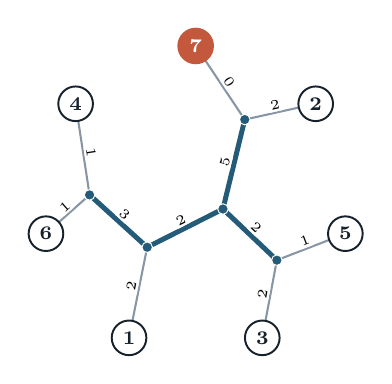
\begin{tikzpicture}[x=1cm,y=1cm]
\coordinate (v1) at (-0.84607,-1.75689);
\coordinate (v2) at (1.52457,1.21581);
\coordinate (v3) at (0.84607,-1.75689);
\coordinate (v4) at (-1.52457,1.21581);
\coordinate (v5) at (1.90111,-0.43392);
\coordinate (v6) at (-1.90111,-0.43392);
\coordinate (v7) at (0.00000,1.95000);
\coordinate (v8) at (0.62367,1.01508);
\coordinate (v9) at (-1.34709,0.05853);
\coordinate (v10) at (-0.61558,-0.60631);
\coordinate (v11) at (1.03121,-0.77046);
\coordinate (v12) at (0.34643,-0.12056);
\draw[internal edge] (v8) -- node[edge label,pos=0.50] {$5$} (v12);
\draw[internal edge] (v9) -- node[edge label,pos=0.50] {$3$} (v10);
\draw[internal edge] (v10) -- node[edge label,pos=0.50] {$2$} (v12);
\draw[internal edge] (v11) -- node[edge label,pos=0.50] {$2$} (v12);
\draw[pendant edge] (v1) -- node[edge label,pos=0.55] {$2$} (v10);
\draw[pendant edge] (v2) -- node[edge label,pos=0.55] {$2$} (v8);
\draw[pendant edge] (v3) -- node[edge label,pos=0.55] {$2$} (v11);
\draw[pendant edge] (v4) -- node[edge label,pos=0.55] {$1$} (v9);
\draw[pendant edge] (v5) -- node[edge label,pos=0.55] {$1$} (v11);
\draw[pendant edge] (v6) -- node[edge label,pos=0.55] {$1$} (v9);
\draw[pendant edge] (v7) -- node[edge label,pos=0.55] {$0$} (v8);
\node[internal vertex] at (v8) {};
\node[internal vertex] at (v9) {};
\node[internal vertex] at (v10) {};
\node[internal vertex] at (v11) {};
\node[internal vertex] at (v12) {};
\node[leaf] at (v1) {1};
\node[leaf] at (v2) {2};
\node[leaf] at (v3) {3};
\node[leaf] at (v4) {4};
\node[leaf] at (v5) {5};
\node[leaf] at (v6) {6};
\node[special leaf] at (v7) {7};
\end{tikzpicture}
\end{minipage}
\hfill
\begin{minipage}[t][0.225\textheight][t]{0.485\textwidth}
\centering
{\normalsize\bfseries Triangle 235}\par
{\small\color{muted} Rays $\{7,\,31,\,51\}$}\par\vspace{0.3mm}
{\scriptsize \textcolor{toricgreen}{\bfseries PRIME TORIC}\color{muted}\quad $\dim/\deg=6/18$\quad GB 42/2}\par
{\scriptsize\color{bodyviolet} $f=(8,\,23,\,32,\,23,\,8)$\quad degree-one/lattice $=14/15$}\par\vspace{0.3mm}
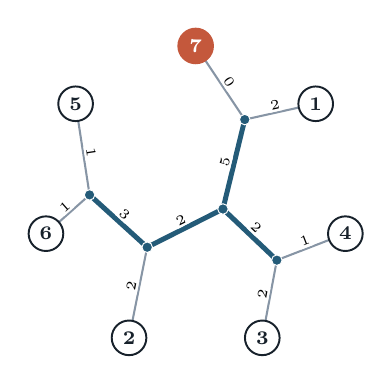
\begin{tikzpicture}[x=1cm,y=1cm]
\coordinate (v1) at (1.52457,1.21581);
\coordinate (v2) at (-0.84607,-1.75689);
\coordinate (v3) at (0.84607,-1.75689);
\coordinate (v4) at (1.90111,-0.43392);
\coordinate (v5) at (-1.52457,1.21581);
\coordinate (v6) at (-1.90111,-0.43392);
\coordinate (v7) at (0.00000,1.95000);
\coordinate (v8) at (0.62367,1.01508);
\coordinate (v9) at (-1.34709,0.05853);
\coordinate (v10) at (-0.61558,-0.60631);
\coordinate (v11) at (1.03121,-0.77046);
\coordinate (v12) at (0.34643,-0.12056);
\draw[internal edge] (v8) -- node[edge label,pos=0.50] {$5$} (v12);
\draw[internal edge] (v9) -- node[edge label,pos=0.50] {$3$} (v10);
\draw[internal edge] (v10) -- node[edge label,pos=0.50] {$2$} (v12);
\draw[internal edge] (v11) -- node[edge label,pos=0.50] {$2$} (v12);
\draw[pendant edge] (v1) -- node[edge label,pos=0.55] {$2$} (v8);
\draw[pendant edge] (v2) -- node[edge label,pos=0.55] {$2$} (v10);
\draw[pendant edge] (v3) -- node[edge label,pos=0.55] {$2$} (v11);
\draw[pendant edge] (v4) -- node[edge label,pos=0.55] {$1$} (v11);
\draw[pendant edge] (v5) -- node[edge label,pos=0.55] {$1$} (v9);
\draw[pendant edge] (v6) -- node[edge label,pos=0.55] {$1$} (v9);
\draw[pendant edge] (v7) -- node[edge label,pos=0.55] {$0$} (v8);
\node[internal vertex] at (v8) {};
\node[internal vertex] at (v9) {};
\node[internal vertex] at (v10) {};
\node[internal vertex] at (v11) {};
\node[internal vertex] at (v12) {};
\node[leaf] at (v1) {1};
\node[leaf] at (v2) {2};
\node[leaf] at (v3) {3};
\node[leaf] at (v4) {4};
\node[leaf] at (v5) {5};
\node[leaf] at (v6) {6};
\node[special leaf] at (v7) {7};
\end{tikzpicture}
\end{minipage}
\par
\begin{minipage}[t][0.225\textheight][t]{0.485\textwidth}
\centering
{\normalsize\bfseries Triangle 250}\par
{\small\color{muted} Rays $\{40,\,46,\,51\}$}\par\vspace{0.3mm}
{\scriptsize \textcolor{nonprimered}{\bfseries NON-PRIME}\color{muted}\quad $\dim/\deg=6/18$\quad GB 53/2}\par
\vspace{1.9mm}
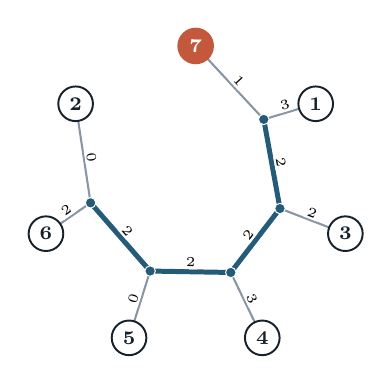
\begin{tikzpicture}[x=1cm,y=1cm]
\coordinate (v1) at (1.52457,1.21581);
\coordinate (v2) at (-1.52457,1.21581);
\coordinate (v3) at (1.90111,-0.43392);
\coordinate (v4) at (0.84607,-1.75689);
\coordinate (v5) at (-0.84607,-1.75689);
\coordinate (v6) at (-1.90111,-0.43392);
\coordinate (v7) at (0.00000,1.95000);
\coordinate (v8) at (0.86513,1.01711);
\coordinate (v9) at (-1.33461,-0.04223);
\coordinate (v10) at (1.07083,-0.11449);
\coordinate (v11) at (0.44625,-0.92666);
\coordinate (v12) at (-0.57814,-0.90859);
\draw[internal edge] (v8) -- node[edge label,pos=0.50] {$2$} (v10);
\draw[internal edge] (v9) -- node[edge label,pos=0.50] {$2$} (v12);
\draw[internal edge] (v10) -- node[edge label,pos=0.50] {$2$} (v11);
\draw[internal edge] (v11) -- node[edge label,pos=0.50] {$2$} (v12);
\draw[pendant edge] (v1) -- node[edge label,pos=0.55] {$3$} (v8);
\draw[pendant edge] (v2) -- node[edge label,pos=0.55] {$0$} (v9);
\draw[pendant edge] (v3) -- node[edge label,pos=0.55] {$2$} (v10);
\draw[pendant edge] (v4) -- node[edge label,pos=0.55] {$3$} (v11);
\draw[pendant edge] (v5) -- node[edge label,pos=0.55] {$0$} (v12);
\draw[pendant edge] (v6) -- node[edge label,pos=0.55] {$2$} (v9);
\draw[pendant edge] (v7) -- node[edge label,pos=0.55] {$1$} (v8);
\node[internal vertex] at (v8) {};
\node[internal vertex] at (v9) {};
\node[internal vertex] at (v10) {};
\node[internal vertex] at (v11) {};
\node[internal vertex] at (v12) {};
\node[leaf] at (v1) {1};
\node[leaf] at (v2) {2};
\node[leaf] at (v3) {3};
\node[leaf] at (v4) {4};
\node[leaf] at (v5) {5};
\node[leaf] at (v6) {6};
\node[special leaf] at (v7) {7};
\end{tikzpicture}
\end{minipage}
\hfill
\begin{minipage}[t][0.225\textheight][t]{0.485\textwidth}
\centering
{\normalsize\bfseries Triangle 251}\par
{\small\color{muted} Rays $\{41,\,47,\,50\}$}\par\vspace{0.3mm}
{\scriptsize \textcolor{nonprimered}{\bfseries NON-PRIME}\color{muted}\quad $\dim/\deg=6/18$\quad GB 45/2}\par
\vspace{1.9mm}
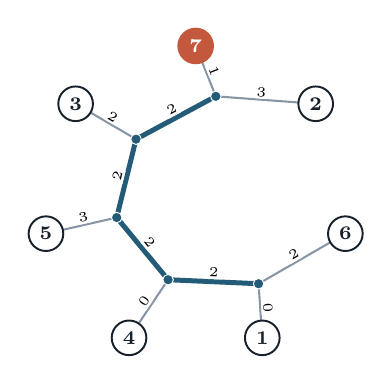
\begin{tikzpicture}[x=1cm,y=1cm]
\coordinate (v1) at (0.84607,-1.75689);
\coordinate (v2) at (1.52457,1.21581);
\coordinate (v3) at (-1.52457,1.21581);
\coordinate (v4) at (-0.84607,-1.75689);
\coordinate (v5) at (-1.90111,-0.43392);
\coordinate (v6) at (1.90111,-0.43392);
\coordinate (v7) at (0.00000,1.95000);
\coordinate (v8) at (0.79909,-1.06977);
\coordinate (v9) at (0.25580,1.31054);
\coordinate (v10) at (-0.75716,0.76583);
\coordinate (v11) at (-0.34990,-1.01851);
\coordinate (v12) at (-1.00273,-0.22887);
\draw[internal edge] (v8) -- node[edge label,pos=0.50] {$2$} (v11);
\draw[internal edge] (v9) -- node[edge label,pos=0.50] {$2$} (v10);
\draw[internal edge] (v10) -- node[edge label,pos=0.50] {$2$} (v12);
\draw[internal edge] (v11) -- node[edge label,pos=0.50] {$2$} (v12);
\draw[pendant edge] (v1) -- node[edge label,pos=0.55] {$0$} (v8);
\draw[pendant edge] (v2) -- node[edge label,pos=0.55] {$3$} (v9);
\draw[pendant edge] (v3) -- node[edge label,pos=0.55] {$2$} (v10);
\draw[pendant edge] (v4) -- node[edge label,pos=0.55] {$0$} (v11);
\draw[pendant edge] (v5) -- node[edge label,pos=0.55] {$3$} (v12);
\draw[pendant edge] (v6) -- node[edge label,pos=0.55] {$2$} (v8);
\draw[pendant edge] (v7) -- node[edge label,pos=0.55] {$1$} (v9);
\node[internal vertex] at (v8) {};
\node[internal vertex] at (v9) {};
\node[internal vertex] at (v10) {};
\node[internal vertex] at (v11) {};
\node[internal vertex] at (v12) {};
\node[leaf] at (v1) {1};
\node[leaf] at (v2) {2};
\node[leaf] at (v3) {3};
\node[leaf] at (v4) {4};
\node[leaf] at (v5) {5};
\node[leaf] at (v6) {6};
\node[special leaf] at (v7) {7};
\end{tikzpicture}
\end{minipage}
\par
\clearpage

\begin{tikzpicture}
\node[rounded corners=2pt,fill=paperblue,inner xsep=5mm,inner ysep=2mm,text width=.94\textwidth] {\Large\bfseries Orbit 3\hfill\normalsize 24 triangles};
\end{tikzpicture}\par\vspace{0.5mm}
{\scriptsize\color{muted} Triangle indices: 5, 6, 7, 8, 47, 48, 90, 91, 114, 115, 116, 117, 178, 179, 196, 197, 198, 201, 202, 203, 239, 242, 246, 247}\par{\scriptsize\color{muted} Algebra: \textcolor{toricgreen}{12 toric}, \textcolor{warningamber}{0 prime non-binomial}, \textcolor{nonprimered}{12 non-prime}.}\par\vspace{1mm}
\begin{minipage}[t][0.225\textheight][t]{0.485\textwidth}
\centering
{\normalsize\bfseries Triangle 5}\par
{\small\color{muted} Rays $\{1,\,2,\,8\}$}\par\vspace{0.3mm}
{\scriptsize \textcolor{nonprimered}{\bfseries NON-PRIME}\color{muted}\quad $\dim/\deg=6/18$\quad GB 37/2}\par
\vspace{1.9mm}
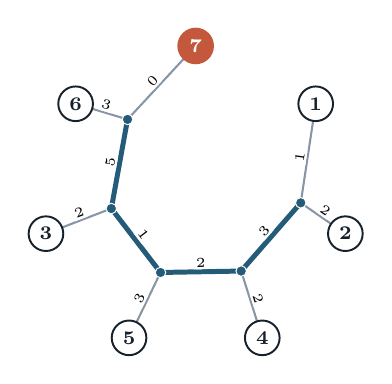
\begin{tikzpicture}[x=1cm,y=1cm]
\coordinate (v1) at (1.52457,1.21581);
\coordinate (v2) at (1.90111,-0.43392);
\coordinate (v3) at (-1.90111,-0.43392);
\coordinate (v4) at (0.84607,-1.75689);
\coordinate (v5) at (-0.84607,-1.75689);
\coordinate (v6) at (-1.52457,1.21581);
\coordinate (v7) at (0.00000,1.95000);
\coordinate (v8) at (-0.86513,1.01711);
\coordinate (v9) at (1.33461,-0.04223);
\coordinate (v10) at (0.57814,-0.90859);
\coordinate (v11) at (-1.07083,-0.11449);
\coordinate (v12) at (-0.44625,-0.92666);
\draw[internal edge] (v8) -- node[edge label,pos=0.50] {$5$} (v11);
\draw[internal edge] (v9) -- node[edge label,pos=0.50] {$3$} (v10);
\draw[internal edge] (v10) -- node[edge label,pos=0.50] {$2$} (v12);
\draw[internal edge] (v11) -- node[edge label,pos=0.50] {$1$} (v12);
\draw[pendant edge] (v1) -- node[edge label,pos=0.55] {$1$} (v9);
\draw[pendant edge] (v2) -- node[edge label,pos=0.55] {$2$} (v9);
\draw[pendant edge] (v3) -- node[edge label,pos=0.55] {$2$} (v11);
\draw[pendant edge] (v4) -- node[edge label,pos=0.55] {$2$} (v10);
\draw[pendant edge] (v5) -- node[edge label,pos=0.55] {$3$} (v12);
\draw[pendant edge] (v6) -- node[edge label,pos=0.55] {$3$} (v8);
\draw[pendant edge] (v7) -- node[edge label,pos=0.55] {$0$} (v8);
\node[internal vertex] at (v8) {};
\node[internal vertex] at (v9) {};
\node[internal vertex] at (v10) {};
\node[internal vertex] at (v11) {};
\node[internal vertex] at (v12) {};
\node[leaf] at (v1) {1};
\node[leaf] at (v2) {2};
\node[leaf] at (v3) {3};
\node[leaf] at (v4) {4};
\node[leaf] at (v5) {5};
\node[leaf] at (v6) {6};
\node[special leaf] at (v7) {7};
\end{tikzpicture}
\end{minipage}
\hfill
\begin{minipage}[t][0.225\textheight][t]{0.485\textwidth}
\centering
{\normalsize\bfseries Triangle 6}\par
{\small\color{muted} Rays $\{2,\,4,\,8\}$}\par\vspace{0.3mm}
{\scriptsize \textcolor{nonprimered}{\bfseries NON-PRIME}\color{muted}\quad $\dim/\deg=6/18$\quad GB 38/2}\par
\vspace{1.9mm}
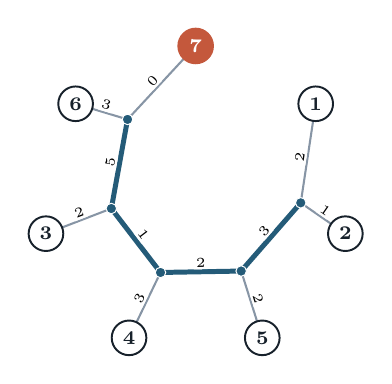
\begin{tikzpicture}[x=1cm,y=1cm]
\coordinate (v1) at (1.52457,1.21581);
\coordinate (v2) at (1.90111,-0.43392);
\coordinate (v3) at (-1.90111,-0.43392);
\coordinate (v4) at (-0.84607,-1.75689);
\coordinate (v5) at (0.84607,-1.75689);
\coordinate (v6) at (-1.52457,1.21581);
\coordinate (v7) at (0.00000,1.95000);
\coordinate (v8) at (-0.86513,1.01711);
\coordinate (v9) at (1.33461,-0.04223);
\coordinate (v10) at (0.57814,-0.90859);
\coordinate (v11) at (-1.07083,-0.11449);
\coordinate (v12) at (-0.44625,-0.92666);
\draw[internal edge] (v8) -- node[edge label,pos=0.50] {$5$} (v11);
\draw[internal edge] (v9) -- node[edge label,pos=0.50] {$3$} (v10);
\draw[internal edge] (v10) -- node[edge label,pos=0.50] {$2$} (v12);
\draw[internal edge] (v11) -- node[edge label,pos=0.50] {$1$} (v12);
\draw[pendant edge] (v1) -- node[edge label,pos=0.55] {$2$} (v9);
\draw[pendant edge] (v2) -- node[edge label,pos=0.55] {$1$} (v9);
\draw[pendant edge] (v3) -- node[edge label,pos=0.55] {$2$} (v11);
\draw[pendant edge] (v4) -- node[edge label,pos=0.55] {$3$} (v12);
\draw[pendant edge] (v5) -- node[edge label,pos=0.55] {$2$} (v10);
\draw[pendant edge] (v6) -- node[edge label,pos=0.55] {$3$} (v8);
\draw[pendant edge] (v7) -- node[edge label,pos=0.55] {$0$} (v8);
\node[internal vertex] at (v8) {};
\node[internal vertex] at (v9) {};
\node[internal vertex] at (v10) {};
\node[internal vertex] at (v11) {};
\node[internal vertex] at (v12) {};
\node[leaf] at (v1) {1};
\node[leaf] at (v2) {2};
\node[leaf] at (v3) {3};
\node[leaf] at (v4) {4};
\node[leaf] at (v5) {5};
\node[leaf] at (v6) {6};
\node[special leaf] at (v7) {7};
\end{tikzpicture}
\end{minipage}
\par
\begin{minipage}[t][0.225\textheight][t]{0.485\textwidth}
\centering
{\normalsize\bfseries Triangle 7}\par
{\small\color{muted} Rays $\{1,\,3,\,9\}$}\par\vspace{0.3mm}
{\scriptsize \textcolor{toricgreen}{\bfseries PRIME TORIC}\color{muted}\quad $\dim/\deg=6/18$\quad GB 35/2}\par
{\scriptsize\color{bodyviolet} $f=(9,\,27,\,38,\,27,\,9)$\quad degree-one/lattice $=14/14$}\par\vspace{0.3mm}
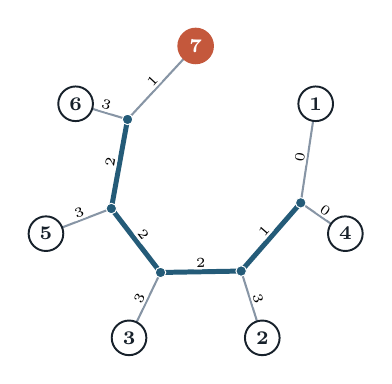
\begin{tikzpicture}[x=1cm,y=1cm]
\coordinate (v1) at (1.52457,1.21581);
\coordinate (v2) at (0.84607,-1.75689);
\coordinate (v3) at (-0.84607,-1.75689);
\coordinate (v4) at (1.90111,-0.43392);
\coordinate (v5) at (-1.90111,-0.43392);
\coordinate (v6) at (-1.52457,1.21581);
\coordinate (v7) at (0.00000,1.95000);
\coordinate (v8) at (-0.86513,1.01711);
\coordinate (v9) at (-1.07083,-0.11449);
\coordinate (v10) at (-0.44625,-0.92666);
\coordinate (v11) at (1.33461,-0.04223);
\coordinate (v12) at (0.57814,-0.90859);
\draw[internal edge] (v8) -- node[edge label,pos=0.50] {$2$} (v9);
\draw[internal edge] (v9) -- node[edge label,pos=0.50] {$2$} (v10);
\draw[internal edge] (v10) -- node[edge label,pos=0.50] {$2$} (v12);
\draw[internal edge] (v11) -- node[edge label,pos=0.50] {$1$} (v12);
\draw[pendant edge] (v1) -- node[edge label,pos=0.55] {$0$} (v11);
\draw[pendant edge] (v2) -- node[edge label,pos=0.55] {$3$} (v12);
\draw[pendant edge] (v3) -- node[edge label,pos=0.55] {$3$} (v10);
\draw[pendant edge] (v4) -- node[edge label,pos=0.55] {$0$} (v11);
\draw[pendant edge] (v5) -- node[edge label,pos=0.55] {$3$} (v9);
\draw[pendant edge] (v6) -- node[edge label,pos=0.55] {$3$} (v8);
\draw[pendant edge] (v7) -- node[edge label,pos=0.55] {$1$} (v8);
\node[internal vertex] at (v8) {};
\node[internal vertex] at (v9) {};
\node[internal vertex] at (v10) {};
\node[internal vertex] at (v11) {};
\node[internal vertex] at (v12) {};
\node[leaf] at (v1) {1};
\node[leaf] at (v2) {2};
\node[leaf] at (v3) {3};
\node[leaf] at (v4) {4};
\node[leaf] at (v5) {5};
\node[leaf] at (v6) {6};
\node[special leaf] at (v7) {7};
\end{tikzpicture}
\end{minipage}
\hfill
\begin{minipage}[t][0.225\textheight][t]{0.485\textwidth}
\centering
{\normalsize\bfseries Triangle 8}\par
{\small\color{muted} Rays $\{4,\,5,\,10\}$}\par\vspace{0.3mm}
{\scriptsize \textcolor{toricgreen}{\bfseries PRIME TORIC}\color{muted}\quad $\dim/\deg=6/18$\quad GB 35/2}\par
{\scriptsize\color{bodyviolet} $f=(9,\,27,\,38,\,27,\,9)$\quad degree-one/lattice $=14/14$}\par\vspace{0.3mm}
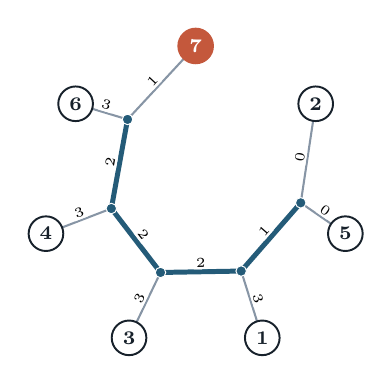
\begin{tikzpicture}[x=1cm,y=1cm]
\coordinate (v1) at (0.84607,-1.75689);
\coordinate (v2) at (1.52457,1.21581);
\coordinate (v3) at (-0.84607,-1.75689);
\coordinate (v4) at (-1.90111,-0.43392);
\coordinate (v5) at (1.90111,-0.43392);
\coordinate (v6) at (-1.52457,1.21581);
\coordinate (v7) at (0.00000,1.95000);
\coordinate (v8) at (-0.86513,1.01711);
\coordinate (v9) at (-1.07083,-0.11449);
\coordinate (v10) at (-0.44625,-0.92666);
\coordinate (v11) at (0.57814,-0.90859);
\coordinate (v12) at (1.33461,-0.04223);
\draw[internal edge] (v8) -- node[edge label,pos=0.50] {$2$} (v9);
\draw[internal edge] (v9) -- node[edge label,pos=0.50] {$2$} (v10);
\draw[internal edge] (v10) -- node[edge label,pos=0.50] {$2$} (v11);
\draw[internal edge] (v11) -- node[edge label,pos=0.50] {$1$} (v12);
\draw[pendant edge] (v1) -- node[edge label,pos=0.55] {$3$} (v11);
\draw[pendant edge] (v2) -- node[edge label,pos=0.55] {$0$} (v12);
\draw[pendant edge] (v3) -- node[edge label,pos=0.55] {$3$} (v10);
\draw[pendant edge] (v4) -- node[edge label,pos=0.55] {$3$} (v9);
\draw[pendant edge] (v5) -- node[edge label,pos=0.55] {$0$} (v12);
\draw[pendant edge] (v6) -- node[edge label,pos=0.55] {$3$} (v8);
\draw[pendant edge] (v7) -- node[edge label,pos=0.55] {$1$} (v8);
\node[internal vertex] at (v8) {};
\node[internal vertex] at (v9) {};
\node[internal vertex] at (v10) {};
\node[internal vertex] at (v11) {};
\node[internal vertex] at (v12) {};
\node[leaf] at (v1) {1};
\node[leaf] at (v2) {2};
\node[leaf] at (v3) {3};
\node[leaf] at (v4) {4};
\node[leaf] at (v5) {5};
\node[leaf] at (v6) {6};
\node[special leaf] at (v7) {7};
\end{tikzpicture}
\end{minipage}
\par
\begin{minipage}[t][0.225\textheight][t]{0.485\textwidth}
\centering
{\normalsize\bfseries Triangle 47}\par
{\small\color{muted} Rays $\{3,\,9,\,23\}$}\par\vspace{0.3mm}
{\scriptsize \textcolor{toricgreen}{\bfseries PRIME TORIC}\color{muted}\quad $\dim/\deg=6/18$\quad GB 38/2}\par
{\scriptsize\color{bodyviolet} $f=(9,\,27,\,38,\,27,\,9)$\quad degree-one/lattice $=14/14$}\par\vspace{0.3mm}
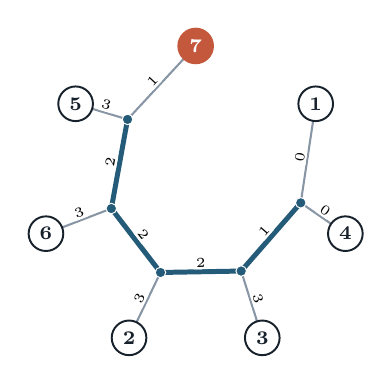
\begin{tikzpicture}[x=1cm,y=1cm]
\coordinate (v1) at (1.52457,1.21581);
\coordinate (v2) at (-0.84607,-1.75689);
\coordinate (v3) at (0.84607,-1.75689);
\coordinate (v4) at (1.90111,-0.43392);
\coordinate (v5) at (-1.52457,1.21581);
\coordinate (v6) at (-1.90111,-0.43392);
\coordinate (v7) at (0.00000,1.95000);
\coordinate (v8) at (-0.86513,1.01711);
\coordinate (v9) at (-1.07083,-0.11449);
\coordinate (v10) at (-0.44625,-0.92666);
\coordinate (v11) at (1.33461,-0.04223);
\coordinate (v12) at (0.57814,-0.90859);
\draw[internal edge] (v8) -- node[edge label,pos=0.50] {$2$} (v9);
\draw[internal edge] (v9) -- node[edge label,pos=0.50] {$2$} (v10);
\draw[internal edge] (v10) -- node[edge label,pos=0.50] {$2$} (v12);
\draw[internal edge] (v11) -- node[edge label,pos=0.50] {$1$} (v12);
\draw[pendant edge] (v1) -- node[edge label,pos=0.55] {$0$} (v11);
\draw[pendant edge] (v2) -- node[edge label,pos=0.55] {$3$} (v10);
\draw[pendant edge] (v3) -- node[edge label,pos=0.55] {$3$} (v12);
\draw[pendant edge] (v4) -- node[edge label,pos=0.55] {$0$} (v11);
\draw[pendant edge] (v5) -- node[edge label,pos=0.55] {$3$} (v8);
\draw[pendant edge] (v6) -- node[edge label,pos=0.55] {$3$} (v9);
\draw[pendant edge] (v7) -- node[edge label,pos=0.55] {$1$} (v8);
\node[internal vertex] at (v8) {};
\node[internal vertex] at (v9) {};
\node[internal vertex] at (v10) {};
\node[internal vertex] at (v11) {};
\node[internal vertex] at (v12) {};
\node[leaf] at (v1) {1};
\node[leaf] at (v2) {2};
\node[leaf] at (v3) {3};
\node[leaf] at (v4) {4};
\node[leaf] at (v5) {5};
\node[leaf] at (v6) {6};
\node[special leaf] at (v7) {7};
\end{tikzpicture}
\end{minipage}
\hfill
\begin{minipage}[t][0.225\textheight][t]{0.485\textwidth}
\centering
{\normalsize\bfseries Triangle 48}\par
{\small\color{muted} Rays $\{5,\,10,\,24\}$}\par\vspace{0.3mm}
{\scriptsize \textcolor{toricgreen}{\bfseries PRIME TORIC}\color{muted}\quad $\dim/\deg=6/18$\quad GB 38/2}\par
{\scriptsize\color{bodyviolet} $f=(9,\,27,\,38,\,27,\,9)$\quad degree-one/lattice $=14/14$}\par\vspace{0.3mm}
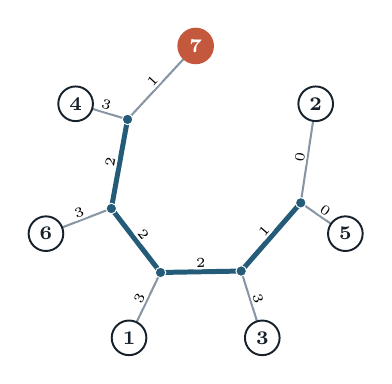
\begin{tikzpicture}[x=1cm,y=1cm]
\coordinate (v1) at (-0.84607,-1.75689);
\coordinate (v2) at (1.52457,1.21581);
\coordinate (v3) at (0.84607,-1.75689);
\coordinate (v4) at (-1.52457,1.21581);
\coordinate (v5) at (1.90111,-0.43392);
\coordinate (v6) at (-1.90111,-0.43392);
\coordinate (v7) at (0.00000,1.95000);
\coordinate (v8) at (-0.86513,1.01711);
\coordinate (v9) at (-1.07083,-0.11449);
\coordinate (v10) at (-0.44625,-0.92666);
\coordinate (v11) at (1.33461,-0.04223);
\coordinate (v12) at (0.57814,-0.90859);
\draw[internal edge] (v8) -- node[edge label,pos=0.50] {$2$} (v9);
\draw[internal edge] (v9) -- node[edge label,pos=0.50] {$2$} (v10);
\draw[internal edge] (v10) -- node[edge label,pos=0.50] {$2$} (v12);
\draw[internal edge] (v11) -- node[edge label,pos=0.50] {$1$} (v12);
\draw[pendant edge] (v1) -- node[edge label,pos=0.55] {$3$} (v10);
\draw[pendant edge] (v2) -- node[edge label,pos=0.55] {$0$} (v11);
\draw[pendant edge] (v3) -- node[edge label,pos=0.55] {$3$} (v12);
\draw[pendant edge] (v4) -- node[edge label,pos=0.55] {$3$} (v8);
\draw[pendant edge] (v5) -- node[edge label,pos=0.55] {$0$} (v11);
\draw[pendant edge] (v6) -- node[edge label,pos=0.55] {$3$} (v9);
\draw[pendant edge] (v7) -- node[edge label,pos=0.55] {$1$} (v8);
\node[internal vertex] at (v8) {};
\node[internal vertex] at (v9) {};
\node[internal vertex] at (v10) {};
\node[internal vertex] at (v11) {};
\node[internal vertex] at (v12) {};
\node[leaf] at (v1) {1};
\node[leaf] at (v2) {2};
\node[leaf] at (v3) {3};
\node[leaf] at (v4) {4};
\node[leaf] at (v5) {5};
\node[leaf] at (v6) {6};
\node[special leaf] at (v7) {7};
\end{tikzpicture}
\end{minipage}
\par
\begin{minipage}[t][0.225\textheight][t]{0.485\textwidth}
\centering
{\normalsize\bfseries Triangle 90}\par
{\small\color{muted} Rays $\{8,\,28,\,42\}$}\par\vspace{0.3mm}
{\scriptsize \textcolor{nonprimered}{\bfseries NON-PRIME}\color{muted}\quad $\dim/\deg=6/18$\quad GB 37/2}\par
\vspace{1.9mm}
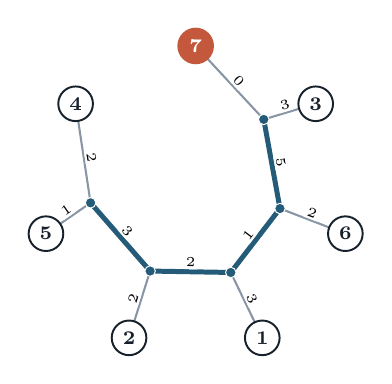
\begin{tikzpicture}[x=1cm,y=1cm]
\coordinate (v1) at (0.84607,-1.75689);
\coordinate (v2) at (-0.84607,-1.75689);
\coordinate (v3) at (1.52457,1.21581);
\coordinate (v4) at (-1.52457,1.21581);
\coordinate (v5) at (-1.90111,-0.43392);
\coordinate (v6) at (1.90111,-0.43392);
\coordinate (v7) at (0.00000,1.95000);
\coordinate (v8) at (0.86513,1.01711);
\coordinate (v9) at (-1.33461,-0.04223);
\coordinate (v10) at (-0.57814,-0.90859);
\coordinate (v11) at (0.44625,-0.92666);
\coordinate (v12) at (1.07083,-0.11449);
\draw[internal edge] (v8) -- node[edge label,pos=0.50] {$5$} (v12);
\draw[internal edge] (v9) -- node[edge label,pos=0.50] {$3$} (v10);
\draw[internal edge] (v10) -- node[edge label,pos=0.50] {$2$} (v11);
\draw[internal edge] (v11) -- node[edge label,pos=0.50] {$1$} (v12);
\draw[pendant edge] (v1) -- node[edge label,pos=0.55] {$3$} (v11);
\draw[pendant edge] (v2) -- node[edge label,pos=0.55] {$2$} (v10);
\draw[pendant edge] (v3) -- node[edge label,pos=0.55] {$3$} (v8);
\draw[pendant edge] (v4) -- node[edge label,pos=0.55] {$2$} (v9);
\draw[pendant edge] (v5) -- node[edge label,pos=0.55] {$1$} (v9);
\draw[pendant edge] (v6) -- node[edge label,pos=0.55] {$2$} (v12);
\draw[pendant edge] (v7) -- node[edge label,pos=0.55] {$0$} (v8);
\node[internal vertex] at (v8) {};
\node[internal vertex] at (v9) {};
\node[internal vertex] at (v10) {};
\node[internal vertex] at (v11) {};
\node[internal vertex] at (v12) {};
\node[leaf] at (v1) {1};
\node[leaf] at (v2) {2};
\node[leaf] at (v3) {3};
\node[leaf] at (v4) {4};
\node[leaf] at (v5) {5};
\node[leaf] at (v6) {6};
\node[special leaf] at (v7) {7};
\end{tikzpicture}
\end{minipage}
\hfill
\begin{minipage}[t][0.225\textheight][t]{0.485\textwidth}
\centering
{\normalsize\bfseries Triangle 91}\par
{\small\color{muted} Rays $\{8,\,28,\,43\}$}\par\vspace{0.3mm}
{\scriptsize \textcolor{nonprimered}{\bfseries NON-PRIME}\color{muted}\quad $\dim/\deg=6/18$\quad GB 37/2}\par
\vspace{1.9mm}
\begin{tikzpicture}[x=1cm,y=1cm]
\coordinate (v1) at (-0.84607,-1.75689);
\coordinate (v2) at (0.84607,-1.75689);
\coordinate (v3) at (1.52457,1.21581);
\coordinate (v4) at (-1.52457,1.21581);
\coordinate (v5) at (-1.90111,-0.43392);
\coordinate (v6) at (1.90111,-0.43392);
\coordinate (v7) at (0.00000,1.95000);
\coordinate (v8) at (0.86513,1.01711);
\coordinate (v9) at (-1.33461,-0.04223);
\coordinate (v10) at (-0.57814,-0.90859);
\coordinate (v11) at (0.44625,-0.92666);
\coordinate (v12) at (1.07083,-0.11449);
\draw[internal edge] (v8) -- node[edge label,pos=0.50] {$5$} (v12);
\draw[internal edge] (v9) -- node[edge label,pos=0.50] {$3$} (v10);
\draw[internal edge] (v10) -- node[edge label,pos=0.50] {$2$} (v11);
\draw[internal edge] (v11) -- node[edge label,pos=0.50] {$1$} (v12);
\draw[pendant edge] (v1) -- node[edge label,pos=0.55] {$2$} (v10);
\draw[pendant edge] (v2) -- node[edge label,pos=0.55] {$3$} (v11);
\draw[pendant edge] (v3) -- node[edge label,pos=0.55] {$3$} (v8);
\draw[pendant edge] (v4) -- node[edge label,pos=0.55] {$1$} (v9);
\draw[pendant edge] (v5) -- node[edge label,pos=0.55] {$2$} (v9);
\draw[pendant edge] (v6) -- node[edge label,pos=0.55] {$2$} (v12);
\draw[pendant edge] (v7) -- node[edge label,pos=0.55] {$0$} (v8);
\node[internal vertex] at (v8) {};
\node[internal vertex] at (v9) {};
\node[internal vertex] at (v10) {};
\node[internal vertex] at (v11) {};
\node[internal vertex] at (v12) {};
\node[leaf] at (v1) {1};
\node[leaf] at (v2) {2};
\node[leaf] at (v3) {3};
\node[leaf] at (v4) {4};
\node[leaf] at (v5) {5};
\node[leaf] at (v6) {6};
\node[special leaf] at (v7) {7};
\end{tikzpicture}
\end{minipage}
\par
\clearpage
\begin{tikzpicture}
\node[rounded corners=2pt,fill=paperblue,inner xsep=5mm,inner ysep=2mm,text width=.94\textwidth] {\Large\bfseries Orbit 3 (continued)\hfill\normalsize 24 triangles};
\end{tikzpicture}\par\vspace{0.5mm}
{\scriptsize\color{muted} Triangle indices: 5, 6, 7, 8, 47, 48, 90, 91, 114, 115, 116, 117, 178, 179, 196, 197, 198, 201, 202, 203, 239, 242, 246, 247}\par{\scriptsize\color{muted} Algebra: \textcolor{toricgreen}{12 toric}, \textcolor{warningamber}{0 prime non-binomial}, \textcolor{nonprimered}{12 non-prime}.}\par\vspace{1mm}
\begin{minipage}[t][0.225\textheight][t]{0.485\textwidth}
\centering
{\normalsize\bfseries Triangle 114}\par
{\small\color{muted} Rays $\{23,\,25,\,33\}$}\par\vspace{0.3mm}
{\scriptsize \textcolor{nonprimered}{\bfseries NON-PRIME}\color{muted}\quad $\dim/\deg=6/18$\quad GB 39/2}\par
\vspace{1.9mm}
\begin{tikzpicture}[x=1cm,y=1cm]
\coordinate (v1) at (1.52457,1.21581);
\coordinate (v2) at (-1.90111,-0.43392);
\coordinate (v3) at (1.90111,-0.43392);
\coordinate (v4) at (0.84607,-1.75689);
\coordinate (v5) at (-1.52457,1.21581);
\coordinate (v6) at (-0.84607,-1.75689);
\coordinate (v7) at (0.00000,1.95000);
\coordinate (v8) at (-0.86513,1.01711);
\coordinate (v9) at (1.33461,-0.04223);
\coordinate (v10) at (0.57814,-0.90859);
\coordinate (v11) at (-1.07083,-0.11449);
\coordinate (v12) at (-0.44625,-0.92666);
\draw[internal edge] (v8) -- node[edge label,pos=0.50] {$5$} (v11);
\draw[internal edge] (v9) -- node[edge label,pos=0.50] {$3$} (v10);
\draw[internal edge] (v10) -- node[edge label,pos=0.50] {$2$} (v12);
\draw[internal edge] (v11) -- node[edge label,pos=0.50] {$1$} (v12);
\draw[pendant edge] (v1) -- node[edge label,pos=0.55] {$1$} (v9);
\draw[pendant edge] (v2) -- node[edge label,pos=0.55] {$2$} (v11);
\draw[pendant edge] (v3) -- node[edge label,pos=0.55] {$2$} (v9);
\draw[pendant edge] (v4) -- node[edge label,pos=0.55] {$2$} (v10);
\draw[pendant edge] (v5) -- node[edge label,pos=0.55] {$3$} (v8);
\draw[pendant edge] (v6) -- node[edge label,pos=0.55] {$3$} (v12);
\draw[pendant edge] (v7) -- node[edge label,pos=0.55] {$0$} (v8);
\node[internal vertex] at (v8) {};
\node[internal vertex] at (v9) {};
\node[internal vertex] at (v10) {};
\node[internal vertex] at (v11) {};
\node[internal vertex] at (v12) {};
\node[leaf] at (v1) {1};
\node[leaf] at (v2) {2};
\node[leaf] at (v3) {3};
\node[leaf] at (v4) {4};
\node[leaf] at (v5) {5};
\node[leaf] at (v6) {6};
\node[special leaf] at (v7) {7};
\end{tikzpicture}
\end{minipage}
\hfill
\begin{minipage}[t][0.225\textheight][t]{0.485\textwidth}
\centering
{\normalsize\bfseries Triangle 115}\par
{\small\color{muted} Rays $\{24,\,26,\,34\}$}\par\vspace{0.3mm}
{\scriptsize \textcolor{nonprimered}{\bfseries NON-PRIME}\color{muted}\quad $\dim/\deg=6/18$\quad GB 39/2}\par
\vspace{1.9mm}
\begin{tikzpicture}[x=1cm,y=1cm]
\coordinate (v1) at (-1.90111,-0.43392);
\coordinate (v2) at (1.52457,1.21581);
\coordinate (v3) at (1.90111,-0.43392);
\coordinate (v4) at (-1.52457,1.21581);
\coordinate (v5) at (0.84607,-1.75689);
\coordinate (v6) at (-0.84607,-1.75689);
\coordinate (v7) at (0.00000,1.95000);
\coordinate (v8) at (-0.86513,1.01711);
\coordinate (v9) at (1.33461,-0.04223);
\coordinate (v10) at (0.57814,-0.90859);
\coordinate (v11) at (-1.07083,-0.11449);
\coordinate (v12) at (-0.44625,-0.92666);
\draw[internal edge] (v8) -- node[edge label,pos=0.50] {$5$} (v11);
\draw[internal edge] (v9) -- node[edge label,pos=0.50] {$3$} (v10);
\draw[internal edge] (v10) -- node[edge label,pos=0.50] {$2$} (v12);
\draw[internal edge] (v11) -- node[edge label,pos=0.50] {$1$} (v12);
\draw[pendant edge] (v1) -- node[edge label,pos=0.55] {$2$} (v11);
\draw[pendant edge] (v2) -- node[edge label,pos=0.55] {$1$} (v9);
\draw[pendant edge] (v3) -- node[edge label,pos=0.55] {$2$} (v9);
\draw[pendant edge] (v4) -- node[edge label,pos=0.55] {$3$} (v8);
\draw[pendant edge] (v5) -- node[edge label,pos=0.55] {$2$} (v10);
\draw[pendant edge] (v6) -- node[edge label,pos=0.55] {$3$} (v12);
\draw[pendant edge] (v7) -- node[edge label,pos=0.55] {$0$} (v8);
\node[internal vertex] at (v8) {};
\node[internal vertex] at (v9) {};
\node[internal vertex] at (v10) {};
\node[internal vertex] at (v11) {};
\node[internal vertex] at (v12) {};
\node[leaf] at (v1) {1};
\node[leaf] at (v2) {2};
\node[leaf] at (v3) {3};
\node[leaf] at (v4) {4};
\node[leaf] at (v5) {5};
\node[leaf] at (v6) {6};
\node[special leaf] at (v7) {7};
\end{tikzpicture}
\end{minipage}
\par
\begin{minipage}[t][0.225\textheight][t]{0.485\textwidth}
\centering
{\normalsize\bfseries Triangle 116}\par
{\small\color{muted} Rays $\{16,\,30,\,38\}$}\par\vspace{0.3mm}
{\scriptsize \textcolor{toricgreen}{\bfseries PRIME TORIC}\color{muted}\quad $\dim/\deg=6/18$\quad GB 39/2}\par
{\scriptsize\color{bodyviolet} $f=(9,\,27,\,38,\,27,\,9)$\quad degree-one/lattice $=14/14$}\par\vspace{0.3mm}
\begin{tikzpicture}[x=1cm,y=1cm]
\coordinate (v1) at (1.90111,-0.43392);
\coordinate (v2) at (1.52457,1.21581);
\coordinate (v3) at (-1.52457,1.21581);
\coordinate (v4) at (-0.84607,-1.75689);
\coordinate (v5) at (0.84607,-1.75689);
\coordinate (v6) at (-1.90111,-0.43392);
\coordinate (v7) at (0.00000,1.95000);
\coordinate (v8) at (0.86513,1.01711);
\coordinate (v9) at (1.07083,-0.11449);
\coordinate (v10) at (0.44625,-0.92666);
\coordinate (v11) at (-1.33461,-0.04223);
\coordinate (v12) at (-0.57814,-0.90859);
\draw[internal edge] (v8) -- node[edge label,pos=0.50] {$2$} (v9);
\draw[internal edge] (v9) -- node[edge label,pos=0.50] {$2$} (v10);
\draw[internal edge] (v10) -- node[edge label,pos=0.50] {$2$} (v12);
\draw[internal edge] (v11) -- node[edge label,pos=0.50] {$1$} (v12);
\draw[pendant edge] (v1) -- node[edge label,pos=0.55] {$3$} (v9);
\draw[pendant edge] (v2) -- node[edge label,pos=0.55] {$3$} (v8);
\draw[pendant edge] (v3) -- node[edge label,pos=0.55] {$0$} (v11);
\draw[pendant edge] (v4) -- node[edge label,pos=0.55] {$3$} (v12);
\draw[pendant edge] (v5) -- node[edge label,pos=0.55] {$3$} (v10);
\draw[pendant edge] (v6) -- node[edge label,pos=0.55] {$0$} (v11);
\draw[pendant edge] (v7) -- node[edge label,pos=0.55] {$1$} (v8);
\node[internal vertex] at (v8) {};
\node[internal vertex] at (v9) {};
\node[internal vertex] at (v10) {};
\node[internal vertex] at (v11) {};
\node[internal vertex] at (v12) {};
\node[leaf] at (v1) {1};
\node[leaf] at (v2) {2};
\node[leaf] at (v3) {3};
\node[leaf] at (v4) {4};
\node[leaf] at (v5) {5};
\node[leaf] at (v6) {6};
\node[special leaf] at (v7) {7};
\end{tikzpicture}
\end{minipage}
\hfill
\begin{minipage}[t][0.225\textheight][t]{0.485\textwidth}
\centering
{\normalsize\bfseries Triangle 117}\par
{\small\color{muted} Rays $\{16,\,30,\,39\}$}\par\vspace{0.3mm}
{\scriptsize \textcolor{toricgreen}{\bfseries PRIME TORIC}\color{muted}\quad $\dim/\deg=6/18$\quad GB 42/2}\par
{\scriptsize\color{bodyviolet} $f=(9,\,27,\,38,\,27,\,9)$\quad degree-one/lattice $=14/14$}\par\vspace{0.3mm}
\begin{tikzpicture}[x=1cm,y=1cm]
\coordinate (v1) at (1.52457,1.21581);
\coordinate (v2) at (1.90111,-0.43392);
\coordinate (v3) at (-1.52457,1.21581);
\coordinate (v4) at (0.84607,-1.75689);
\coordinate (v5) at (-0.84607,-1.75689);
\coordinate (v6) at (-1.90111,-0.43392);
\coordinate (v7) at (0.00000,1.95000);
\coordinate (v8) at (0.86513,1.01711);
\coordinate (v9) at (1.07083,-0.11449);
\coordinate (v10) at (0.44625,-0.92666);
\coordinate (v11) at (-1.33461,-0.04223);
\coordinate (v12) at (-0.57814,-0.90859);
\draw[internal edge] (v8) -- node[edge label,pos=0.50] {$2$} (v9);
\draw[internal edge] (v9) -- node[edge label,pos=0.50] {$2$} (v10);
\draw[internal edge] (v10) -- node[edge label,pos=0.50] {$2$} (v12);
\draw[internal edge] (v11) -- node[edge label,pos=0.50] {$1$} (v12);
\draw[pendant edge] (v1) -- node[edge label,pos=0.55] {$3$} (v8);
\draw[pendant edge] (v2) -- node[edge label,pos=0.55] {$3$} (v9);
\draw[pendant edge] (v3) -- node[edge label,pos=0.55] {$0$} (v11);
\draw[pendant edge] (v4) -- node[edge label,pos=0.55] {$3$} (v10);
\draw[pendant edge] (v5) -- node[edge label,pos=0.55] {$3$} (v12);
\draw[pendant edge] (v6) -- node[edge label,pos=0.55] {$0$} (v11);
\draw[pendant edge] (v7) -- node[edge label,pos=0.55] {$1$} (v8);
\node[internal vertex] at (v8) {};
\node[internal vertex] at (v9) {};
\node[internal vertex] at (v10) {};
\node[internal vertex] at (v11) {};
\node[internal vertex] at (v12) {};
\node[leaf] at (v1) {1};
\node[leaf] at (v2) {2};
\node[leaf] at (v3) {3};
\node[leaf] at (v4) {4};
\node[leaf] at (v5) {5};
\node[leaf] at (v6) {6};
\node[special leaf] at (v7) {7};
\end{tikzpicture}
\end{minipage}
\par
\begin{minipage}[t][0.225\textheight][t]{0.485\textwidth}
\centering
{\normalsize\bfseries Triangle 178}\par
{\small\color{muted} Rays $\{27,\,30,\,48\}$}\par\vspace{0.3mm}
{\scriptsize \textcolor{toricgreen}{\bfseries PRIME TORIC}\color{muted}\quad $\dim/\deg=6/18$\quad GB 36/2}\par
{\scriptsize\color{bodyviolet} $f=(9,\,27,\,38,\,27,\,9)$\quad degree-one/lattice $=14/14$}\par\vspace{0.3mm}
\begin{tikzpicture}[x=1cm,y=1cm]
\coordinate (v1) at (0.84607,-1.75689);
\coordinate (v2) at (-0.84607,-1.75689);
\coordinate (v3) at (1.52457,1.21581);
\coordinate (v4) at (-1.90111,-0.43392);
\coordinate (v5) at (-1.52457,1.21581);
\coordinate (v6) at (1.90111,-0.43392);
\coordinate (v7) at (0.00000,1.95000);
\coordinate (v8) at (-0.86513,1.01711);
\coordinate (v9) at (-1.07083,-0.11449);
\coordinate (v10) at (-0.44625,-0.92666);
\coordinate (v11) at (0.57814,-0.90859);
\coordinate (v12) at (1.33461,-0.04223);
\draw[internal edge] (v8) -- node[edge label,pos=0.50] {$2$} (v9);
\draw[internal edge] (v9) -- node[edge label,pos=0.50] {$2$} (v10);
\draw[internal edge] (v10) -- node[edge label,pos=0.50] {$2$} (v11);
\draw[internal edge] (v11) -- node[edge label,pos=0.50] {$1$} (v12);
\draw[pendant edge] (v1) -- node[edge label,pos=0.55] {$3$} (v11);
\draw[pendant edge] (v2) -- node[edge label,pos=0.55] {$3$} (v10);
\draw[pendant edge] (v3) -- node[edge label,pos=0.55] {$0$} (v12);
\draw[pendant edge] (v4) -- node[edge label,pos=0.55] {$3$} (v9);
\draw[pendant edge] (v5) -- node[edge label,pos=0.55] {$3$} (v8);
\draw[pendant edge] (v6) -- node[edge label,pos=0.55] {$0$} (v12);
\draw[pendant edge] (v7) -- node[edge label,pos=0.55] {$1$} (v8);
\node[internal vertex] at (v8) {};
\node[internal vertex] at (v9) {};
\node[internal vertex] at (v10) {};
\node[internal vertex] at (v11) {};
\node[internal vertex] at (v12) {};
\node[leaf] at (v1) {1};
\node[leaf] at (v2) {2};
\node[leaf] at (v3) {3};
\node[leaf] at (v4) {4};
\node[leaf] at (v5) {5};
\node[leaf] at (v6) {6};
\node[special leaf] at (v7) {7};
\end{tikzpicture}
\end{minipage}
\hfill
\begin{minipage}[t][0.225\textheight][t]{0.485\textwidth}
\centering
{\normalsize\bfseries Triangle 179}\par
{\small\color{muted} Rays $\{27,\,30,\,49\}$}\par\vspace{0.3mm}
{\scriptsize \textcolor{toricgreen}{\bfseries PRIME TORIC}\color{muted}\quad $\dim/\deg=6/18$\quad GB 36/2}\par
{\scriptsize\color{bodyviolet} $f=(9,\,27,\,38,\,27,\,9)$\quad degree-one/lattice $=14/14$}\par\vspace{0.3mm}
\begin{tikzpicture}[x=1cm,y=1cm]
\coordinate (v1) at (-0.84607,-1.75689);
\coordinate (v2) at (0.84607,-1.75689);
\coordinate (v3) at (1.52457,1.21581);
\coordinate (v4) at (-1.52457,1.21581);
\coordinate (v5) at (-1.90111,-0.43392);
\coordinate (v6) at (1.90111,-0.43392);
\coordinate (v7) at (0.00000,1.95000);
\coordinate (v8) at (-0.86513,1.01711);
\coordinate (v9) at (-1.07083,-0.11449);
\coordinate (v10) at (-0.44625,-0.92666);
\coordinate (v11) at (0.57814,-0.90859);
\coordinate (v12) at (1.33461,-0.04223);
\draw[internal edge] (v8) -- node[edge label,pos=0.50] {$2$} (v9);
\draw[internal edge] (v9) -- node[edge label,pos=0.50] {$2$} (v10);
\draw[internal edge] (v10) -- node[edge label,pos=0.50] {$2$} (v11);
\draw[internal edge] (v11) -- node[edge label,pos=0.50] {$1$} (v12);
\draw[pendant edge] (v1) -- node[edge label,pos=0.55] {$3$} (v10);
\draw[pendant edge] (v2) -- node[edge label,pos=0.55] {$3$} (v11);
\draw[pendant edge] (v3) -- node[edge label,pos=0.55] {$0$} (v12);
\draw[pendant edge] (v4) -- node[edge label,pos=0.55] {$3$} (v8);
\draw[pendant edge] (v5) -- node[edge label,pos=0.55] {$3$} (v9);
\draw[pendant edge] (v6) -- node[edge label,pos=0.55] {$0$} (v12);
\draw[pendant edge] (v7) -- node[edge label,pos=0.55] {$1$} (v8);
\node[internal vertex] at (v8) {};
\node[internal vertex] at (v9) {};
\node[internal vertex] at (v10) {};
\node[internal vertex] at (v11) {};
\node[internal vertex] at (v12) {};
\node[leaf] at (v1) {1};
\node[leaf] at (v2) {2};
\node[leaf] at (v3) {3};
\node[leaf] at (v4) {4};
\node[leaf] at (v5) {5};
\node[leaf] at (v6) {6};
\node[special leaf] at (v7) {7};
\end{tikzpicture}
\end{minipage}
\par
\begin{minipage}[t][0.225\textheight][t]{0.485\textwidth}
\centering
{\normalsize\bfseries Triangle 196}\par
{\small\color{muted} Rays $\{25,\,33,\,48\}$}\par\vspace{0.3mm}
{\scriptsize \textcolor{nonprimered}{\bfseries NON-PRIME}\color{muted}\quad $\dim/\deg=6/18$\quad GB 38/2}\par
\vspace{1.9mm}
\begin{tikzpicture}[x=1cm,y=1cm]
\coordinate (v1) at (1.52457,1.21581);
\coordinate (v2) at (-1.90111,-0.43392);
\coordinate (v3) at (1.90111,-0.43392);
\coordinate (v4) at (-0.84607,-1.75689);
\coordinate (v5) at (-1.52457,1.21581);
\coordinate (v6) at (0.84607,-1.75689);
\coordinate (v7) at (0.00000,1.95000);
\coordinate (v8) at (-0.86513,1.01711);
\coordinate (v9) at (1.33461,-0.04223);
\coordinate (v10) at (0.57814,-0.90859);
\coordinate (v11) at (-1.07083,-0.11449);
\coordinate (v12) at (-0.44625,-0.92666);
\draw[internal edge] (v8) -- node[edge label,pos=0.50] {$5$} (v11);
\draw[internal edge] (v9) -- node[edge label,pos=0.50] {$3$} (v10);
\draw[internal edge] (v10) -- node[edge label,pos=0.50] {$2$} (v12);
\draw[internal edge] (v11) -- node[edge label,pos=0.50] {$1$} (v12);
\draw[pendant edge] (v1) -- node[edge label,pos=0.55] {$2$} (v9);
\draw[pendant edge] (v2) -- node[edge label,pos=0.55] {$2$} (v11);
\draw[pendant edge] (v3) -- node[edge label,pos=0.55] {$1$} (v9);
\draw[pendant edge] (v4) -- node[edge label,pos=0.55] {$3$} (v12);
\draw[pendant edge] (v5) -- node[edge label,pos=0.55] {$3$} (v8);
\draw[pendant edge] (v6) -- node[edge label,pos=0.55] {$2$} (v10);
\draw[pendant edge] (v7) -- node[edge label,pos=0.55] {$0$} (v8);
\node[internal vertex] at (v8) {};
\node[internal vertex] at (v9) {};
\node[internal vertex] at (v10) {};
\node[internal vertex] at (v11) {};
\node[internal vertex] at (v12) {};
\node[leaf] at (v1) {1};
\node[leaf] at (v2) {2};
\node[leaf] at (v3) {3};
\node[leaf] at (v4) {4};
\node[leaf] at (v5) {5};
\node[leaf] at (v6) {6};
\node[special leaf] at (v7) {7};
\end{tikzpicture}
\end{minipage}
\hfill
\begin{minipage}[t][0.225\textheight][t]{0.485\textwidth}
\centering
{\normalsize\bfseries Triangle 197}\par
{\small\color{muted} Rays $\{32,\,33,\,38\}$}\par\vspace{0.3mm}
{\scriptsize \textcolor{nonprimered}{\bfseries NON-PRIME}\color{muted}\quad $\dim/\deg=6/18$\quad GB 39/2}\par
\vspace{1.9mm}
\begin{tikzpicture}[x=1cm,y=1cm]
\coordinate (v1) at (0.84607,-1.75689);
\coordinate (v2) at (1.52457,1.21581);
\coordinate (v3) at (-0.84607,-1.75689);
\coordinate (v4) at (-1.52457,1.21581);
\coordinate (v5) at (1.90111,-0.43392);
\coordinate (v6) at (-1.90111,-0.43392);
\coordinate (v7) at (0.00000,1.95000);
\coordinate (v8) at (0.86513,1.01711);
\coordinate (v9) at (-1.33461,-0.04223);
\coordinate (v10) at (-0.57814,-0.90859);
\coordinate (v11) at (0.44625,-0.92666);
\coordinate (v12) at (1.07083,-0.11449);
\draw[internal edge] (v8) -- node[edge label,pos=0.50] {$5$} (v12);
\draw[internal edge] (v9) -- node[edge label,pos=0.50] {$3$} (v10);
\draw[internal edge] (v10) -- node[edge label,pos=0.50] {$2$} (v11);
\draw[internal edge] (v11) -- node[edge label,pos=0.50] {$1$} (v12);
\draw[pendant edge] (v1) -- node[edge label,pos=0.55] {$3$} (v11);
\draw[pendant edge] (v2) -- node[edge label,pos=0.55] {$3$} (v8);
\draw[pendant edge] (v3) -- node[edge label,pos=0.55] {$2$} (v10);
\draw[pendant edge] (v4) -- node[edge label,pos=0.55] {$2$} (v9);
\draw[pendant edge] (v5) -- node[edge label,pos=0.55] {$2$} (v12);
\draw[pendant edge] (v6) -- node[edge label,pos=0.55] {$1$} (v9);
\draw[pendant edge] (v7) -- node[edge label,pos=0.55] {$0$} (v8);
\node[internal vertex] at (v8) {};
\node[internal vertex] at (v9) {};
\node[internal vertex] at (v10) {};
\node[internal vertex] at (v11) {};
\node[internal vertex] at (v12) {};
\node[leaf] at (v1) {1};
\node[leaf] at (v2) {2};
\node[leaf] at (v3) {3};
\node[leaf] at (v4) {4};
\node[leaf] at (v5) {5};
\node[leaf] at (v6) {6};
\node[special leaf] at (v7) {7};
\end{tikzpicture}
\end{minipage}
\par
\clearpage
\begin{tikzpicture}
\node[rounded corners=2pt,fill=paperblue,inner xsep=5mm,inner ysep=2mm,text width=.94\textwidth] {\Large\bfseries Orbit 3 (continued)\hfill\normalsize 24 triangles};
\end{tikzpicture}\par\vspace{0.5mm}
{\scriptsize\color{muted} Triangle indices: 5, 6, 7, 8, 47, 48, 90, 91, 114, 115, 116, 117, 178, 179, 196, 197, 198, 201, 202, 203, 239, 242, 246, 247}\par{\scriptsize\color{muted} Algebra: \textcolor{toricgreen}{12 toric}, \textcolor{warningamber}{0 prime non-binomial}, \textcolor{nonprimered}{12 non-prime}.}\par\vspace{1mm}
\begin{minipage}[t][0.225\textheight][t]{0.485\textwidth}
\centering
{\normalsize\bfseries Triangle 198}\par
{\small\color{muted} Rays $\{26,\,34,\,49\}$}\par\vspace{0.3mm}
{\scriptsize \textcolor{nonprimered}{\bfseries NON-PRIME}\color{muted}\quad $\dim/\deg=6/18$\quad GB 41/2}\par
\vspace{1.9mm}
\begin{tikzpicture}[x=1cm,y=1cm]
\coordinate (v1) at (-1.90111,-0.43392);
\coordinate (v2) at (1.52457,1.21581);
\coordinate (v3) at (1.90111,-0.43392);
\coordinate (v4) at (-1.52457,1.21581);
\coordinate (v5) at (-0.84607,-1.75689);
\coordinate (v6) at (0.84607,-1.75689);
\coordinate (v7) at (0.00000,1.95000);
\coordinate (v8) at (-0.86513,1.01711);
\coordinate (v9) at (1.33461,-0.04223);
\coordinate (v10) at (0.57814,-0.90859);
\coordinate (v11) at (-1.07083,-0.11449);
\coordinate (v12) at (-0.44625,-0.92666);
\draw[internal edge] (v8) -- node[edge label,pos=0.50] {$5$} (v11);
\draw[internal edge] (v9) -- node[edge label,pos=0.50] {$3$} (v10);
\draw[internal edge] (v10) -- node[edge label,pos=0.50] {$2$} (v12);
\draw[internal edge] (v11) -- node[edge label,pos=0.50] {$1$} (v12);
\draw[pendant edge] (v1) -- node[edge label,pos=0.55] {$2$} (v11);
\draw[pendant edge] (v2) -- node[edge label,pos=0.55] {$2$} (v9);
\draw[pendant edge] (v3) -- node[edge label,pos=0.55] {$1$} (v9);
\draw[pendant edge] (v4) -- node[edge label,pos=0.55] {$3$} (v8);
\draw[pendant edge] (v5) -- node[edge label,pos=0.55] {$3$} (v12);
\draw[pendant edge] (v6) -- node[edge label,pos=0.55] {$2$} (v10);
\draw[pendant edge] (v7) -- node[edge label,pos=0.55] {$0$} (v8);
\node[internal vertex] at (v8) {};
\node[internal vertex] at (v9) {};
\node[internal vertex] at (v10) {};
\node[internal vertex] at (v11) {};
\node[internal vertex] at (v12) {};
\node[leaf] at (v1) {1};
\node[leaf] at (v2) {2};
\node[leaf] at (v3) {3};
\node[leaf] at (v4) {4};
\node[leaf] at (v5) {5};
\node[leaf] at (v6) {6};
\node[special leaf] at (v7) {7};
\end{tikzpicture}
\end{minipage}
\hfill
\begin{minipage}[t][0.225\textheight][t]{0.485\textwidth}
\centering
{\normalsize\bfseries Triangle 201}\par
{\small\color{muted} Rays $\{31,\,34,\,39\}$}\par\vspace{0.3mm}
{\scriptsize \textcolor{nonprimered}{\bfseries NON-PRIME}\color{muted}\quad $\dim/\deg=6/18$\quad GB 38/2}\par
\vspace{1.9mm}
\begin{tikzpicture}[x=1cm,y=1cm]
\coordinate (v1) at (1.52457,1.21581);
\coordinate (v2) at (0.84607,-1.75689);
\coordinate (v3) at (-0.84607,-1.75689);
\coordinate (v4) at (1.90111,-0.43392);
\coordinate (v5) at (-1.52457,1.21581);
\coordinate (v6) at (-1.90111,-0.43392);
\coordinate (v7) at (0.00000,1.95000);
\coordinate (v8) at (0.86513,1.01711);
\coordinate (v9) at (-1.33461,-0.04223);
\coordinate (v10) at (-0.57814,-0.90859);
\coordinate (v11) at (0.44625,-0.92666);
\coordinate (v12) at (1.07083,-0.11449);
\draw[internal edge] (v8) -- node[edge label,pos=0.50] {$5$} (v12);
\draw[internal edge] (v9) -- node[edge label,pos=0.50] {$3$} (v10);
\draw[internal edge] (v10) -- node[edge label,pos=0.50] {$2$} (v11);
\draw[internal edge] (v11) -- node[edge label,pos=0.50] {$1$} (v12);
\draw[pendant edge] (v1) -- node[edge label,pos=0.55] {$3$} (v8);
\draw[pendant edge] (v2) -- node[edge label,pos=0.55] {$3$} (v11);
\draw[pendant edge] (v3) -- node[edge label,pos=0.55] {$2$} (v10);
\draw[pendant edge] (v4) -- node[edge label,pos=0.55] {$2$} (v12);
\draw[pendant edge] (v5) -- node[edge label,pos=0.55] {$2$} (v9);
\draw[pendant edge] (v6) -- node[edge label,pos=0.55] {$1$} (v9);
\draw[pendant edge] (v7) -- node[edge label,pos=0.55] {$0$} (v8);
\node[internal vertex] at (v8) {};
\node[internal vertex] at (v9) {};
\node[internal vertex] at (v10) {};
\node[internal vertex] at (v11) {};
\node[internal vertex] at (v12) {};
\node[leaf] at (v1) {1};
\node[leaf] at (v2) {2};
\node[leaf] at (v3) {3};
\node[leaf] at (v4) {4};
\node[leaf] at (v5) {5};
\node[leaf] at (v6) {6};
\node[special leaf] at (v7) {7};
\end{tikzpicture}
\end{minipage}
\par
\begin{minipage}[t][0.225\textheight][t]{0.485\textwidth}
\centering
{\normalsize\bfseries Triangle 202}\par
{\small\color{muted} Rays $\{10,\,42,\,46\}$}\par\vspace{0.3mm}
{\scriptsize \textcolor{toricgreen}{\bfseries PRIME TORIC}\color{muted}\quad $\dim/\deg=6/18$\quad GB 36/2}\par
{\scriptsize\color{bodyviolet} $f=(9,\,27,\,38,\,27,\,9)$\quad degree-one/lattice $=14/14$}\par\vspace{0.3mm}
\begin{tikzpicture}[x=1cm,y=1cm]
\coordinate (v1) at (-1.90111,-0.43392);
\coordinate (v2) at (1.52457,1.21581);
\coordinate (v3) at (-1.52457,1.21581);
\coordinate (v4) at (0.84607,-1.75689);
\coordinate (v5) at (1.90111,-0.43392);
\coordinate (v6) at (-0.84607,-1.75689);
\coordinate (v7) at (0.00000,1.95000);
\coordinate (v8) at (-0.86513,1.01711);
\coordinate (v9) at (-1.07083,-0.11449);
\coordinate (v10) at (-0.44625,-0.92666);
\coordinate (v11) at (1.33461,-0.04223);
\coordinate (v12) at (0.57814,-0.90859);
\draw[internal edge] (v8) -- node[edge label,pos=0.50] {$2$} (v9);
\draw[internal edge] (v9) -- node[edge label,pos=0.50] {$2$} (v10);
\draw[internal edge] (v10) -- node[edge label,pos=0.50] {$2$} (v12);
\draw[internal edge] (v11) -- node[edge label,pos=0.50] {$1$} (v12);
\draw[pendant edge] (v1) -- node[edge label,pos=0.55] {$3$} (v9);
\draw[pendant edge] (v2) -- node[edge label,pos=0.55] {$0$} (v11);
\draw[pendant edge] (v3) -- node[edge label,pos=0.55] {$3$} (v8);
\draw[pendant edge] (v4) -- node[edge label,pos=0.55] {$3$} (v12);
\draw[pendant edge] (v5) -- node[edge label,pos=0.55] {$0$} (v11);
\draw[pendant edge] (v6) -- node[edge label,pos=0.55] {$3$} (v10);
\draw[pendant edge] (v7) -- node[edge label,pos=0.55] {$1$} (v8);
\node[internal vertex] at (v8) {};
\node[internal vertex] at (v9) {};
\node[internal vertex] at (v10) {};
\node[internal vertex] at (v11) {};
\node[internal vertex] at (v12) {};
\node[leaf] at (v1) {1};
\node[leaf] at (v2) {2};
\node[leaf] at (v3) {3};
\node[leaf] at (v4) {4};
\node[leaf] at (v5) {5};
\node[leaf] at (v6) {6};
\node[special leaf] at (v7) {7};
\end{tikzpicture}
\end{minipage}
\hfill
\begin{minipage}[t][0.225\textheight][t]{0.485\textwidth}
\centering
{\normalsize\bfseries Triangle 203}\par
{\small\color{muted} Rays $\{9,\,43,\,47\}$}\par\vspace{0.3mm}
{\scriptsize \textcolor{toricgreen}{\bfseries PRIME TORIC}\color{muted}\quad $\dim/\deg=6/18$\quad GB 35/2}\par
{\scriptsize\color{bodyviolet} $f=(9,\,27,\,38,\,27,\,9)$\quad degree-one/lattice $=14/14$}\par\vspace{0.3mm}
\begin{tikzpicture}[x=1cm,y=1cm]
\coordinate (v1) at (1.52457,1.21581);
\coordinate (v2) at (-1.90111,-0.43392);
\coordinate (v3) at (-1.52457,1.21581);
\coordinate (v4) at (1.90111,-0.43392);
\coordinate (v5) at (0.84607,-1.75689);
\coordinate (v6) at (-0.84607,-1.75689);
\coordinate (v7) at (0.00000,1.95000);
\coordinate (v8) at (-0.86513,1.01711);
\coordinate (v9) at (-1.07083,-0.11449);
\coordinate (v10) at (-0.44625,-0.92666);
\coordinate (v11) at (1.33461,-0.04223);
\coordinate (v12) at (0.57814,-0.90859);
\draw[internal edge] (v8) -- node[edge label,pos=0.50] {$2$} (v9);
\draw[internal edge] (v9) -- node[edge label,pos=0.50] {$2$} (v10);
\draw[internal edge] (v10) -- node[edge label,pos=0.50] {$2$} (v12);
\draw[internal edge] (v11) -- node[edge label,pos=0.50] {$1$} (v12);
\draw[pendant edge] (v1) -- node[edge label,pos=0.55] {$0$} (v11);
\draw[pendant edge] (v2) -- node[edge label,pos=0.55] {$3$} (v9);
\draw[pendant edge] (v3) -- node[edge label,pos=0.55] {$3$} (v8);
\draw[pendant edge] (v4) -- node[edge label,pos=0.55] {$0$} (v11);
\draw[pendant edge] (v5) -- node[edge label,pos=0.55] {$3$} (v12);
\draw[pendant edge] (v6) -- node[edge label,pos=0.55] {$3$} (v10);
\draw[pendant edge] (v7) -- node[edge label,pos=0.55] {$1$} (v8);
\node[internal vertex] at (v8) {};
\node[internal vertex] at (v9) {};
\node[internal vertex] at (v10) {};
\node[internal vertex] at (v11) {};
\node[internal vertex] at (v12) {};
\node[leaf] at (v1) {1};
\node[leaf] at (v2) {2};
\node[leaf] at (v3) {3};
\node[leaf] at (v4) {4};
\node[leaf] at (v5) {5};
\node[leaf] at (v6) {6};
\node[special leaf] at (v7) {7};
\end{tikzpicture}
\end{minipage}
\par
\begin{minipage}[t][0.225\textheight][t]{0.485\textwidth}
\centering
{\normalsize\bfseries Triangle 239}\par
{\small\color{muted} Rays $\{32,\,33,\,50\}$}\par\vspace{0.3mm}
{\scriptsize \textcolor{nonprimered}{\bfseries NON-PRIME}\color{muted}\quad $\dim/\deg=6/18$\quad GB 40/2}\par
\vspace{1.9mm}
\begin{tikzpicture}[x=1cm,y=1cm]
\coordinate (v1) at (-0.84607,-1.75689);
\coordinate (v2) at (1.52457,1.21581);
\coordinate (v3) at (0.84607,-1.75689);
\coordinate (v4) at (-1.52457,1.21581);
\coordinate (v5) at (1.90111,-0.43392);
\coordinate (v6) at (-1.90111,-0.43392);
\coordinate (v7) at (0.00000,1.95000);
\coordinate (v8) at (0.86513,1.01711);
\coordinate (v9) at (-1.33461,-0.04223);
\coordinate (v10) at (-0.57814,-0.90859);
\coordinate (v11) at (0.44625,-0.92666);
\coordinate (v12) at (1.07083,-0.11449);
\draw[internal edge] (v8) -- node[edge label,pos=0.50] {$5$} (v12);
\draw[internal edge] (v9) -- node[edge label,pos=0.50] {$3$} (v10);
\draw[internal edge] (v10) -- node[edge label,pos=0.50] {$2$} (v11);
\draw[internal edge] (v11) -- node[edge label,pos=0.50] {$1$} (v12);
\draw[pendant edge] (v1) -- node[edge label,pos=0.55] {$2$} (v10);
\draw[pendant edge] (v2) -- node[edge label,pos=0.55] {$3$} (v8);
\draw[pendant edge] (v3) -- node[edge label,pos=0.55] {$3$} (v11);
\draw[pendant edge] (v4) -- node[edge label,pos=0.55] {$1$} (v9);
\draw[pendant edge] (v5) -- node[edge label,pos=0.55] {$2$} (v12);
\draw[pendant edge] (v6) -- node[edge label,pos=0.55] {$2$} (v9);
\draw[pendant edge] (v7) -- node[edge label,pos=0.55] {$0$} (v8);
\node[internal vertex] at (v8) {};
\node[internal vertex] at (v9) {};
\node[internal vertex] at (v10) {};
\node[internal vertex] at (v11) {};
\node[internal vertex] at (v12) {};
\node[leaf] at (v1) {1};
\node[leaf] at (v2) {2};
\node[leaf] at (v3) {3};
\node[leaf] at (v4) {4};
\node[leaf] at (v5) {5};
\node[leaf] at (v6) {6};
\node[special leaf] at (v7) {7};
\end{tikzpicture}
\end{minipage}
\hfill
\begin{minipage}[t][0.225\textheight][t]{0.485\textwidth}
\centering
{\normalsize\bfseries Triangle 242}\par
{\small\color{muted} Rays $\{31,\,34,\,51\}$}\par\vspace{0.3mm}
{\scriptsize \textcolor{nonprimered}{\bfseries NON-PRIME}\color{muted}\quad $\dim/\deg=6/18$\quad GB 40/2}\par
\vspace{1.9mm}
\begin{tikzpicture}[x=1cm,y=1cm]
\coordinate (v1) at (1.52457,1.21581);
\coordinate (v2) at (-0.84607,-1.75689);
\coordinate (v3) at (0.84607,-1.75689);
\coordinate (v4) at (1.90111,-0.43392);
\coordinate (v5) at (-1.52457,1.21581);
\coordinate (v6) at (-1.90111,-0.43392);
\coordinate (v7) at (0.00000,1.95000);
\coordinate (v8) at (0.86513,1.01711);
\coordinate (v9) at (-1.33461,-0.04223);
\coordinate (v10) at (-0.57814,-0.90859);
\coordinate (v11) at (0.44625,-0.92666);
\coordinate (v12) at (1.07083,-0.11449);
\draw[internal edge] (v8) -- node[edge label,pos=0.50] {$5$} (v12);
\draw[internal edge] (v9) -- node[edge label,pos=0.50] {$3$} (v10);
\draw[internal edge] (v10) -- node[edge label,pos=0.50] {$2$} (v11);
\draw[internal edge] (v11) -- node[edge label,pos=0.50] {$1$} (v12);
\draw[pendant edge] (v1) -- node[edge label,pos=0.55] {$3$} (v8);
\draw[pendant edge] (v2) -- node[edge label,pos=0.55] {$2$} (v10);
\draw[pendant edge] (v3) -- node[edge label,pos=0.55] {$3$} (v11);
\draw[pendant edge] (v4) -- node[edge label,pos=0.55] {$2$} (v12);
\draw[pendant edge] (v5) -- node[edge label,pos=0.55] {$1$} (v9);
\draw[pendant edge] (v6) -- node[edge label,pos=0.55] {$2$} (v9);
\draw[pendant edge] (v7) -- node[edge label,pos=0.55] {$0$} (v8);
\node[internal vertex] at (v8) {};
\node[internal vertex] at (v9) {};
\node[internal vertex] at (v10) {};
\node[internal vertex] at (v11) {};
\node[internal vertex] at (v12) {};
\node[leaf] at (v1) {1};
\node[leaf] at (v2) {2};
\node[leaf] at (v3) {3};
\node[leaf] at (v4) {4};
\node[leaf] at (v5) {5};
\node[leaf] at (v6) {6};
\node[special leaf] at (v7) {7};
\end{tikzpicture}
\end{minipage}
\par
\begin{minipage}[t][0.225\textheight][t]{0.485\textwidth}
\centering
{\normalsize\bfseries Triangle 246}\par
{\small\color{muted} Rays $\{10,\,46,\,51\}$}\par\vspace{0.3mm}
{\scriptsize \textcolor{toricgreen}{\bfseries PRIME TORIC}\color{muted}\quad $\dim/\deg=6/18$\quad GB 44/2}\par
{\scriptsize\color{bodyviolet} $f=(9,\,27,\,38,\,27,\,9)$\quad degree-one/lattice $=14/14$}\par\vspace{0.3mm}
\begin{tikzpicture}[x=1cm,y=1cm]
\coordinate (v1) at (1.52457,1.21581);
\coordinate (v2) at (-1.52457,1.21581);
\coordinate (v3) at (1.90111,-0.43392);
\coordinate (v4) at (0.84607,-1.75689);
\coordinate (v5) at (-1.90111,-0.43392);
\coordinate (v6) at (-0.84607,-1.75689);
\coordinate (v7) at (0.00000,1.95000);
\coordinate (v8) at (0.86513,1.01711);
\coordinate (v9) at (1.07083,-0.11449);
\coordinate (v10) at (0.44625,-0.92666);
\coordinate (v11) at (-1.33461,-0.04223);
\coordinate (v12) at (-0.57814,-0.90859);
\draw[internal edge] (v8) -- node[edge label,pos=0.50] {$2$} (v9);
\draw[internal edge] (v9) -- node[edge label,pos=0.50] {$2$} (v10);
\draw[internal edge] (v10) -- node[edge label,pos=0.50] {$2$} (v12);
\draw[internal edge] (v11) -- node[edge label,pos=0.50] {$1$} (v12);
\draw[pendant edge] (v1) -- node[edge label,pos=0.55] {$3$} (v8);
\draw[pendant edge] (v2) -- node[edge label,pos=0.55] {$0$} (v11);
\draw[pendant edge] (v3) -- node[edge label,pos=0.55] {$3$} (v9);
\draw[pendant edge] (v4) -- node[edge label,pos=0.55] {$3$} (v10);
\draw[pendant edge] (v5) -- node[edge label,pos=0.55] {$0$} (v11);
\draw[pendant edge] (v6) -- node[edge label,pos=0.55] {$3$} (v12);
\draw[pendant edge] (v7) -- node[edge label,pos=0.55] {$1$} (v8);
\node[internal vertex] at (v8) {};
\node[internal vertex] at (v9) {};
\node[internal vertex] at (v10) {};
\node[internal vertex] at (v11) {};
\node[internal vertex] at (v12) {};
\node[leaf] at (v1) {1};
\node[leaf] at (v2) {2};
\node[leaf] at (v3) {3};
\node[leaf] at (v4) {4};
\node[leaf] at (v5) {5};
\node[leaf] at (v6) {6};
\node[special leaf] at (v7) {7};
\end{tikzpicture}
\end{minipage}
\hfill
\begin{minipage}[t][0.225\textheight][t]{0.485\textwidth}
\centering
{\normalsize\bfseries Triangle 247}\par
{\small\color{muted} Rays $\{9,\,47,\,50\}$}\par\vspace{0.3mm}
{\scriptsize \textcolor{toricgreen}{\bfseries PRIME TORIC}\color{muted}\quad $\dim/\deg=6/18$\quad GB 40/2}\par
{\scriptsize\color{bodyviolet} $f=(9,\,27,\,38,\,27,\,9)$\quad degree-one/lattice $=14/14$}\par\vspace{0.3mm}
\begin{tikzpicture}[x=1cm,y=1cm]
\coordinate (v1) at (1.52457,1.21581);
\coordinate (v2) at (-1.52457,1.21581);
\coordinate (v3) at (-1.90111,-0.43392);
\coordinate (v4) at (1.90111,-0.43392);
\coordinate (v5) at (-0.84607,-1.75689);
\coordinate (v6) at (0.84607,-1.75689);
\coordinate (v7) at (0.00000,1.95000);
\coordinate (v8) at (-0.86513,1.01711);
\coordinate (v9) at (-1.07083,-0.11449);
\coordinate (v10) at (-0.44625,-0.92666);
\coordinate (v11) at (1.33461,-0.04223);
\coordinate (v12) at (0.57814,-0.90859);
\draw[internal edge] (v8) -- node[edge label,pos=0.50] {$2$} (v9);
\draw[internal edge] (v9) -- node[edge label,pos=0.50] {$2$} (v10);
\draw[internal edge] (v10) -- node[edge label,pos=0.50] {$2$} (v12);
\draw[internal edge] (v11) -- node[edge label,pos=0.50] {$1$} (v12);
\draw[pendant edge] (v1) -- node[edge label,pos=0.55] {$0$} (v11);
\draw[pendant edge] (v2) -- node[edge label,pos=0.55] {$3$} (v8);
\draw[pendant edge] (v3) -- node[edge label,pos=0.55] {$3$} (v9);
\draw[pendant edge] (v4) -- node[edge label,pos=0.55] {$0$} (v11);
\draw[pendant edge] (v5) -- node[edge label,pos=0.55] {$3$} (v10);
\draw[pendant edge] (v6) -- node[edge label,pos=0.55] {$3$} (v12);
\draw[pendant edge] (v7) -- node[edge label,pos=0.55] {$1$} (v8);
\node[internal vertex] at (v8) {};
\node[internal vertex] at (v9) {};
\node[internal vertex] at (v10) {};
\node[internal vertex] at (v11) {};
\node[internal vertex] at (v12) {};
\node[leaf] at (v1) {1};
\node[leaf] at (v2) {2};
\node[leaf] at (v3) {3};
\node[leaf] at (v4) {4};
\node[leaf] at (v5) {5};
\node[leaf] at (v6) {6};
\node[special leaf] at (v7) {7};
\end{tikzpicture}
\end{minipage}
\par
\clearpage
\begin{tikzpicture}
\node[rounded corners=2pt,fill=paperblue,inner xsep=5mm,inner ysep=2mm,text width=.94\textwidth] {\Large\bfseries Orbit 4\hfill\normalsize 12 triangles};
\end{tikzpicture}\par\vspace{0.5mm}
{\scriptsize\color{muted} Triangle indices: 11, 12, 53, 54, 65, 66, 146, 148, 222, 223, 224, 225}\par{\scriptsize\color{muted} Algebra: \textcolor{toricgreen}{0 toric}, \textcolor{warningamber}{0 prime non-binomial}, \textcolor{nonprimered}{12 non-prime}.}\par\vspace{1mm}
\begin{minipage}[t][0.225\textheight][t]{0.485\textwidth}
\centering
{\normalsize\bfseries Triangle 11}\par
{\small\color{muted} Rays $\{2,\,3,\,7\}$}\par\vspace{0.3mm}
{\scriptsize \textcolor{nonprimered}{\bfseries NON-PRIME}\color{muted}\quad $\dim/\deg=6/18$\quad GB 35/2}\par
\vspace{1.9mm}
\begin{tikzpicture}[x=1cm,y=1cm]
\coordinate (v1) at (1.52457,1.21581);
\coordinate (v2) at (1.90111,-0.43392);
\coordinate (v3) at (0.84607,-1.75689);
\coordinate (v4) at (-0.84607,-1.75689);
\coordinate (v5) at (-1.90111,-0.43392);
\coordinate (v6) at (-1.52457,1.21581);
\coordinate (v7) at (0.00000,1.95000);
\coordinate (v8) at (-0.79414,1.08968);
\coordinate (v9) at (1.18247,0.14529);
\coordinate (v10) at (0.04058,-1.28660);
\coordinate (v11) at (-0.85784,0.10325);
\coordinate (v12) at (0.12174,-0.34602);
\draw[internal edge] (v8) -- node[edge label,pos=0.50] {$3$} (v11);
\draw[internal edge] (v9) -- node[edge label,pos=0.50] {$3$} (v12);
\draw[internal edge] (v10) -- node[edge label,pos=0.50] {$2$} (v12);
\draw[internal edge] (v11) -- node[edge label,pos=0.50] {$2$} (v12);
\draw[pendant edge] (v1) -- node[edge label,pos=0.55] {$0$} (v9);
\draw[pendant edge] (v2) -- node[edge label,pos=0.55] {$2$} (v9);
\draw[pendant edge] (v3) -- node[edge label,pos=0.55] {$1$} (v10);
\draw[pendant edge] (v4) -- node[edge label,pos=0.55] {$1$} (v10);
\draw[pendant edge] (v5) -- node[edge label,pos=0.55] {$3$} (v11);
\draw[pendant edge] (v6) -- node[edge label,pos=0.55] {$2$} (v8);
\draw[pendant edge] (v7) -- node[edge label,pos=0.55] {$0$} (v8);
\node[internal vertex] at (v8) {};
\node[internal vertex] at (v9) {};
\node[internal vertex] at (v10) {};
\node[internal vertex] at (v11) {};
\node[internal vertex] at (v12) {};
\node[leaf] at (v1) {1};
\node[leaf] at (v2) {2};
\node[leaf] at (v3) {3};
\node[leaf] at (v4) {4};
\node[leaf] at (v5) {5};
\node[leaf] at (v6) {6};
\node[special leaf] at (v7) {7};
\end{tikzpicture}
\end{minipage}
\hfill
\begin{minipage}[t][0.225\textheight][t]{0.485\textwidth}
\centering
{\normalsize\bfseries Triangle 12}\par
{\small\color{muted} Rays $\{2,\,5,\,6\}$}\par\vspace{0.3mm}
{\scriptsize \textcolor{nonprimered}{\bfseries NON-PRIME}\color{muted}\quad $\dim/\deg=6/18$\quad GB 37/2}\par
\vspace{1.9mm}
\begin{tikzpicture}[x=1cm,y=1cm]
\coordinate (v1) at (1.52457,1.21581);
\coordinate (v2) at (1.90111,-0.43392);
\coordinate (v3) at (0.84607,-1.75689);
\coordinate (v4) at (-1.90111,-0.43392);
\coordinate (v5) at (-0.84607,-1.75689);
\coordinate (v6) at (-1.52457,1.21581);
\coordinate (v7) at (0.00000,1.95000);
\coordinate (v8) at (-0.79414,1.08968);
\coordinate (v9) at (1.18247,0.14529);
\coordinate (v10) at (0.04058,-1.28660);
\coordinate (v11) at (-0.85784,0.10325);
\coordinate (v12) at (0.12174,-0.34602);
\draw[internal edge] (v8) -- node[edge label,pos=0.50] {$3$} (v11);
\draw[internal edge] (v9) -- node[edge label,pos=0.50] {$3$} (v12);
\draw[internal edge] (v10) -- node[edge label,pos=0.50] {$2$} (v12);
\draw[internal edge] (v11) -- node[edge label,pos=0.50] {$2$} (v12);
\draw[pendant edge] (v1) -- node[edge label,pos=0.55] {$2$} (v9);
\draw[pendant edge] (v2) -- node[edge label,pos=0.55] {$0$} (v9);
\draw[pendant edge] (v3) -- node[edge label,pos=0.55] {$1$} (v10);
\draw[pendant edge] (v4) -- node[edge label,pos=0.55] {$3$} (v11);
\draw[pendant edge] (v5) -- node[edge label,pos=0.55] {$1$} (v10);
\draw[pendant edge] (v6) -- node[edge label,pos=0.55] {$2$} (v8);
\draw[pendant edge] (v7) -- node[edge label,pos=0.55] {$0$} (v8);
\node[internal vertex] at (v8) {};
\node[internal vertex] at (v9) {};
\node[internal vertex] at (v10) {};
\node[internal vertex] at (v11) {};
\node[internal vertex] at (v12) {};
\node[leaf] at (v1) {1};
\node[leaf] at (v2) {2};
\node[leaf] at (v3) {3};
\node[leaf] at (v4) {4};
\node[leaf] at (v5) {5};
\node[leaf] at (v6) {6};
\node[special leaf] at (v7) {7};
\end{tikzpicture}
\end{minipage}
\par
\begin{minipage}[t][0.225\textheight][t]{0.485\textwidth}
\centering
{\normalsize\bfseries Triangle 53}\par
{\small\color{muted} Rays $\{3,\,11,\,25\}$}\par\vspace{0.3mm}
{\scriptsize \textcolor{nonprimered}{\bfseries NON-PRIME}\color{muted}\quad $\dim/\deg=6/18$\quad GB 35/2}\par
\vspace{1.9mm}
\begin{tikzpicture}[x=1cm,y=1cm]
\coordinate (v1) at (1.52457,1.21581);
\coordinate (v2) at (0.84607,-1.75689);
\coordinate (v3) at (1.90111,-0.43392);
\coordinate (v4) at (-0.84607,-1.75689);
\coordinate (v5) at (-1.52457,1.21581);
\coordinate (v6) at (-1.90111,-0.43392);
\coordinate (v7) at (0.00000,1.95000);
\coordinate (v8) at (-0.79414,1.08968);
\coordinate (v9) at (1.18247,0.14529);
\coordinate (v10) at (0.04058,-1.28660);
\coordinate (v11) at (-0.85784,0.10325);
\coordinate (v12) at (0.12174,-0.34602);
\draw[internal edge] (v8) -- node[edge label,pos=0.50] {$3$} (v11);
\draw[internal edge] (v9) -- node[edge label,pos=0.50] {$3$} (v12);
\draw[internal edge] (v10) -- node[edge label,pos=0.50] {$2$} (v12);
\draw[internal edge] (v11) -- node[edge label,pos=0.50] {$2$} (v12);
\draw[pendant edge] (v1) -- node[edge label,pos=0.55] {$0$} (v9);
\draw[pendant edge] (v2) -- node[edge label,pos=0.55] {$1$} (v10);
\draw[pendant edge] (v3) -- node[edge label,pos=0.55] {$2$} (v9);
\draw[pendant edge] (v4) -- node[edge label,pos=0.55] {$1$} (v10);
\draw[pendant edge] (v5) -- node[edge label,pos=0.55] {$2$} (v8);
\draw[pendant edge] (v6) -- node[edge label,pos=0.55] {$3$} (v11);
\draw[pendant edge] (v7) -- node[edge label,pos=0.55] {$0$} (v8);
\node[internal vertex] at (v8) {};
\node[internal vertex] at (v9) {};
\node[internal vertex] at (v10) {};
\node[internal vertex] at (v11) {};
\node[internal vertex] at (v12) {};
\node[leaf] at (v1) {1};
\node[leaf] at (v2) {2};
\node[leaf] at (v3) {3};
\node[leaf] at (v4) {4};
\node[leaf] at (v5) {5};
\node[leaf] at (v6) {6};
\node[special leaf] at (v7) {7};
\end{tikzpicture}
\end{minipage}
\hfill
\begin{minipage}[t][0.225\textheight][t]{0.485\textwidth}
\centering
{\normalsize\bfseries Triangle 54}\par
{\small\color{muted} Rays $\{5,\,12,\,26\}$}\par\vspace{0.3mm}
{\scriptsize \textcolor{nonprimered}{\bfseries NON-PRIME}\color{muted}\quad $\dim/\deg=6/18$\quad GB 35/2}\par
\vspace{1.9mm}
\begin{tikzpicture}[x=1cm,y=1cm]
\coordinate (v1) at (1.52457,1.21581);
\coordinate (v2) at (0.84607,-1.75689);
\coordinate (v3) at (-0.84607,-1.75689);
\coordinate (v4) at (-1.52457,1.21581);
\coordinate (v5) at (1.90111,-0.43392);
\coordinate (v6) at (-1.90111,-0.43392);
\coordinate (v7) at (0.00000,1.95000);
\coordinate (v8) at (-0.79414,1.08968);
\coordinate (v9) at (0.04058,-1.28660);
\coordinate (v10) at (1.18247,0.14529);
\coordinate (v11) at (-0.85784,0.10325);
\coordinate (v12) at (0.12174,-0.34602);
\draw[internal edge] (v8) -- node[edge label,pos=0.50] {$3$} (v11);
\draw[internal edge] (v9) -- node[edge label,pos=0.50] {$3$} (v12);
\draw[internal edge] (v10) -- node[edge label,pos=0.50] {$2$} (v12);
\draw[internal edge] (v11) -- node[edge label,pos=0.50] {$2$} (v12);
\draw[pendant edge] (v1) -- node[edge label,pos=0.55] {$1$} (v10);
\draw[pendant edge] (v2) -- node[edge label,pos=0.55] {$0$} (v9);
\draw[pendant edge] (v3) -- node[edge label,pos=0.55] {$2$} (v9);
\draw[pendant edge] (v4) -- node[edge label,pos=0.55] {$2$} (v8);
\draw[pendant edge] (v5) -- node[edge label,pos=0.55] {$1$} (v10);
\draw[pendant edge] (v6) -- node[edge label,pos=0.55] {$3$} (v11);
\draw[pendant edge] (v7) -- node[edge label,pos=0.55] {$0$} (v8);
\node[internal vertex] at (v8) {};
\node[internal vertex] at (v9) {};
\node[internal vertex] at (v10) {};
\node[internal vertex] at (v11) {};
\node[internal vertex] at (v12) {};
\node[leaf] at (v1) {1};
\node[leaf] at (v2) {2};
\node[leaf] at (v3) {3};
\node[leaf] at (v4) {4};
\node[leaf] at (v5) {5};
\node[leaf] at (v6) {6};
\node[special leaf] at (v7) {7};
\end{tikzpicture}
\end{minipage}
\par
\begin{minipage}[t][0.225\textheight][t]{0.485\textwidth}
\centering
{\normalsize\bfseries Triangle 65}\par
{\small\color{muted} Rays $\{7,\,16,\,31\}$}\par\vspace{0.3mm}
{\scriptsize \textcolor{nonprimered}{\bfseries NON-PRIME}\color{muted}\quad $\dim/\deg=6/18$\quad GB 37/2}\par
\vspace{1.9mm}
\begin{tikzpicture}[x=1cm,y=1cm]
\coordinate (v1) at (1.52457,1.21581);
\coordinate (v2) at (1.90111,-0.43392);
\coordinate (v3) at (-1.52457,1.21581);
\coordinate (v4) at (-1.90111,-0.43392);
\coordinate (v5) at (-0.84607,-1.75689);
\coordinate (v6) at (0.84607,-1.75689);
\coordinate (v7) at (0.00000,1.95000);
\coordinate (v8) at (0.79414,1.08968);
\coordinate (v9) at (-0.04058,-1.28660);
\coordinate (v10) at (0.85784,0.10325);
\coordinate (v11) at (-1.18247,0.14529);
\coordinate (v12) at (-0.12174,-0.34602);
\draw[internal edge] (v8) -- node[edge label,pos=0.50] {$3$} (v10);
\draw[internal edge] (v9) -- node[edge label,pos=0.50] {$3$} (v12);
\draw[internal edge] (v10) -- node[edge label,pos=0.50] {$2$} (v12);
\draw[internal edge] (v11) -- node[edge label,pos=0.50] {$2$} (v12);
\draw[pendant edge] (v1) -- node[edge label,pos=0.55] {$2$} (v8);
\draw[pendant edge] (v2) -- node[edge label,pos=0.55] {$3$} (v10);
\draw[pendant edge] (v3) -- node[edge label,pos=0.55] {$1$} (v11);
\draw[pendant edge] (v4) -- node[edge label,pos=0.55] {$1$} (v11);
\draw[pendant edge] (v5) -- node[edge label,pos=0.55] {$2$} (v9);
\draw[pendant edge] (v6) -- node[edge label,pos=0.55] {$0$} (v9);
\draw[pendant edge] (v7) -- node[edge label,pos=0.55] {$0$} (v8);
\node[internal vertex] at (v8) {};
\node[internal vertex] at (v9) {};
\node[internal vertex] at (v10) {};
\node[internal vertex] at (v11) {};
\node[internal vertex] at (v12) {};
\node[leaf] at (v1) {1};
\node[leaf] at (v2) {2};
\node[leaf] at (v3) {3};
\node[leaf] at (v4) {4};
\node[leaf] at (v5) {5};
\node[leaf] at (v6) {6};
\node[special leaf] at (v7) {7};
\end{tikzpicture}
\end{minipage}
\hfill
\begin{minipage}[t][0.225\textheight][t]{0.485\textwidth}
\centering
{\normalsize\bfseries Triangle 66}\par
{\small\color{muted} Rays $\{6,\,16,\,32\}$}\par\vspace{0.3mm}
{\scriptsize \textcolor{nonprimered}{\bfseries NON-PRIME}\color{muted}\quad $\dim/\deg=6/18$\quad GB 39/2}\par
\vspace{1.9mm}
\begin{tikzpicture}[x=1cm,y=1cm]
\coordinate (v1) at (1.90111,-0.43392);
\coordinate (v2) at (1.52457,1.21581);
\coordinate (v3) at (-1.52457,1.21581);
\coordinate (v4) at (-0.84607,-1.75689);
\coordinate (v5) at (-1.90111,-0.43392);
\coordinate (v6) at (0.84607,-1.75689);
\coordinate (v7) at (0.00000,1.95000);
\coordinate (v8) at (0.79414,1.08968);
\coordinate (v9) at (-0.04058,-1.28660);
\coordinate (v10) at (0.85784,0.10325);
\coordinate (v11) at (-1.18247,0.14529);
\coordinate (v12) at (-0.12174,-0.34602);
\draw[internal edge] (v8) -- node[edge label,pos=0.50] {$3$} (v10);
\draw[internal edge] (v9) -- node[edge label,pos=0.50] {$3$} (v12);
\draw[internal edge] (v10) -- node[edge label,pos=0.50] {$2$} (v12);
\draw[internal edge] (v11) -- node[edge label,pos=0.50] {$2$} (v12);
\draw[pendant edge] (v1) -- node[edge label,pos=0.55] {$3$} (v10);
\draw[pendant edge] (v2) -- node[edge label,pos=0.55] {$2$} (v8);
\draw[pendant edge] (v3) -- node[edge label,pos=0.55] {$1$} (v11);
\draw[pendant edge] (v4) -- node[edge label,pos=0.55] {$2$} (v9);
\draw[pendant edge] (v5) -- node[edge label,pos=0.55] {$1$} (v11);
\draw[pendant edge] (v6) -- node[edge label,pos=0.55] {$0$} (v9);
\draw[pendant edge] (v7) -- node[edge label,pos=0.55] {$0$} (v8);
\node[internal vertex] at (v8) {};
\node[internal vertex] at (v9) {};
\node[internal vertex] at (v10) {};
\node[internal vertex] at (v11) {};
\node[internal vertex] at (v12) {};
\node[leaf] at (v1) {1};
\node[leaf] at (v2) {2};
\node[leaf] at (v3) {3};
\node[leaf] at (v4) {4};
\node[leaf] at (v5) {5};
\node[leaf] at (v6) {6};
\node[special leaf] at (v7) {7};
\end{tikzpicture}
\end{minipage}
\par
\begin{minipage}[t][0.225\textheight][t]{0.485\textwidth}
\centering
{\normalsize\bfseries Triangle 146}\par
{\small\color{muted} Rays $\{25,\,27,\,40\}$}\par\vspace{0.3mm}
{\scriptsize \textcolor{nonprimered}{\bfseries NON-PRIME}\color{muted}\quad $\dim/\deg=6/18$\quad GB 38/2}\par
\vspace{1.9mm}
\begin{tikzpicture}[x=1cm,y=1cm]
\coordinate (v1) at (1.52457,1.21581);
\coordinate (v2) at (0.84607,-1.75689);
\coordinate (v3) at (1.90111,-0.43392);
\coordinate (v4) at (-1.90111,-0.43392);
\coordinate (v5) at (-1.52457,1.21581);
\coordinate (v6) at (-0.84607,-1.75689);
\coordinate (v7) at (0.00000,1.95000);
\coordinate (v8) at (-0.79414,1.08968);
\coordinate (v9) at (1.18247,0.14529);
\coordinate (v10) at (0.04058,-1.28660);
\coordinate (v11) at (-0.85784,0.10325);
\coordinate (v12) at (0.12174,-0.34602);
\draw[internal edge] (v8) -- node[edge label,pos=0.50] {$3$} (v11);
\draw[internal edge] (v9) -- node[edge label,pos=0.50] {$3$} (v12);
\draw[internal edge] (v10) -- node[edge label,pos=0.50] {$2$} (v12);
\draw[internal edge] (v11) -- node[edge label,pos=0.50] {$2$} (v12);
\draw[pendant edge] (v1) -- node[edge label,pos=0.55] {$2$} (v9);
\draw[pendant edge] (v2) -- node[edge label,pos=0.55] {$1$} (v10);
\draw[pendant edge] (v3) -- node[edge label,pos=0.55] {$0$} (v9);
\draw[pendant edge] (v4) -- node[edge label,pos=0.55] {$3$} (v11);
\draw[pendant edge] (v5) -- node[edge label,pos=0.55] {$2$} (v8);
\draw[pendant edge] (v6) -- node[edge label,pos=0.55] {$1$} (v10);
\draw[pendant edge] (v7) -- node[edge label,pos=0.55] {$0$} (v8);
\node[internal vertex] at (v8) {};
\node[internal vertex] at (v9) {};
\node[internal vertex] at (v10) {};
\node[internal vertex] at (v11) {};
\node[internal vertex] at (v12) {};
\node[leaf] at (v1) {1};
\node[leaf] at (v2) {2};
\node[leaf] at (v3) {3};
\node[leaf] at (v4) {4};
\node[leaf] at (v5) {5};
\node[leaf] at (v6) {6};
\node[special leaf] at (v7) {7};
\end{tikzpicture}
\end{minipage}
\hfill
\begin{minipage}[t][0.225\textheight][t]{0.485\textwidth}
\centering
{\normalsize\bfseries Triangle 148}\par
{\small\color{muted} Rays $\{26,\,27,\,41\}$}\par\vspace{0.3mm}
{\scriptsize \textcolor{nonprimered}{\bfseries NON-PRIME}\color{muted}\quad $\dim/\deg=6/18$\quad GB 38/2}\par
\vspace{1.9mm}
\begin{tikzpicture}[x=1cm,y=1cm]
\coordinate (v1) at (1.52457,1.21581);
\coordinate (v2) at (0.84607,-1.75689);
\coordinate (v3) at (-0.84607,-1.75689);
\coordinate (v4) at (-1.52457,1.21581);
\coordinate (v5) at (-1.90111,-0.43392);
\coordinate (v6) at (1.90111,-0.43392);
\coordinate (v7) at (0.00000,1.95000);
\coordinate (v8) at (-0.79414,1.08968);
\coordinate (v9) at (0.04058,-1.28660);
\coordinate (v10) at (1.18247,0.14529);
\coordinate (v11) at (-0.85784,0.10325);
\coordinate (v12) at (0.12174,-0.34602);
\draw[internal edge] (v8) -- node[edge label,pos=0.50] {$3$} (v11);
\draw[internal edge] (v9) -- node[edge label,pos=0.50] {$3$} (v12);
\draw[internal edge] (v10) -- node[edge label,pos=0.50] {$2$} (v12);
\draw[internal edge] (v11) -- node[edge label,pos=0.50] {$2$} (v12);
\draw[pendant edge] (v1) -- node[edge label,pos=0.55] {$1$} (v10);
\draw[pendant edge] (v2) -- node[edge label,pos=0.55] {$2$} (v9);
\draw[pendant edge] (v3) -- node[edge label,pos=0.55] {$0$} (v9);
\draw[pendant edge] (v4) -- node[edge label,pos=0.55] {$2$} (v8);
\draw[pendant edge] (v5) -- node[edge label,pos=0.55] {$3$} (v11);
\draw[pendant edge] (v6) -- node[edge label,pos=0.55] {$1$} (v10);
\draw[pendant edge] (v7) -- node[edge label,pos=0.55] {$0$} (v8);
\node[internal vertex] at (v8) {};
\node[internal vertex] at (v9) {};
\node[internal vertex] at (v10) {};
\node[internal vertex] at (v11) {};
\node[internal vertex] at (v12) {};
\node[leaf] at (v1) {1};
\node[leaf] at (v2) {2};
\node[leaf] at (v3) {3};
\node[leaf] at (v4) {4};
\node[leaf] at (v5) {5};
\node[leaf] at (v6) {6};
\node[special leaf] at (v7) {7};
\end{tikzpicture}
\end{minipage}
\par
\clearpage
\begin{tikzpicture}
\node[rounded corners=2pt,fill=paperblue,inner xsep=5mm,inner ysep=2mm,text width=.94\textwidth] {\Large\bfseries Orbit 4 (continued)\hfill\normalsize 12 triangles};
\end{tikzpicture}\par\vspace{0.5mm}
{\scriptsize\color{muted} Triangle indices: 11, 12, 53, 54, 65, 66, 146, 148, 222, 223, 224, 225}\par{\scriptsize\color{muted} Algebra: \textcolor{toricgreen}{0 toric}, \textcolor{warningamber}{0 prime non-binomial}, \textcolor{nonprimered}{12 non-prime}.}\par\vspace{1mm}
\begin{minipage}[t][0.225\textheight][t]{0.485\textwidth}
\centering
{\normalsize\bfseries Triangle 222}\par
{\small\color{muted} Rays $\{11,\,31,\,46\}$}\par\vspace{0.3mm}
{\scriptsize \textcolor{nonprimered}{\bfseries NON-PRIME}\color{muted}\quad $\dim/\deg=6/18$\quad GB 40/2}\par
\vspace{1.9mm}
\begin{tikzpicture}[x=1cm,y=1cm]
\coordinate (v1) at (1.52457,1.21581);
\coordinate (v2) at (-1.52457,1.21581);
\coordinate (v3) at (1.90111,-0.43392);
\coordinate (v4) at (-1.90111,-0.43392);
\coordinate (v5) at (-0.84607,-1.75689);
\coordinate (v6) at (0.84607,-1.75689);
\coordinate (v7) at (0.00000,1.95000);
\coordinate (v8) at (0.79414,1.08968);
\coordinate (v9) at (-0.04058,-1.28660);
\coordinate (v10) at (-1.18247,0.14529);
\coordinate (v11) at (0.85784,0.10325);
\coordinate (v12) at (-0.12174,-0.34602);
\draw[internal edge] (v8) -- node[edge label,pos=0.50] {$3$} (v11);
\draw[internal edge] (v9) -- node[edge label,pos=0.50] {$3$} (v12);
\draw[internal edge] (v10) -- node[edge label,pos=0.50] {$2$} (v12);
\draw[internal edge] (v11) -- node[edge label,pos=0.50] {$2$} (v12);
\draw[pendant edge] (v1) -- node[edge label,pos=0.55] {$2$} (v8);
\draw[pendant edge] (v2) -- node[edge label,pos=0.55] {$1$} (v10);
\draw[pendant edge] (v3) -- node[edge label,pos=0.55] {$3$} (v11);
\draw[pendant edge] (v4) -- node[edge label,pos=0.55] {$1$} (v10);
\draw[pendant edge] (v5) -- node[edge label,pos=0.55] {$0$} (v9);
\draw[pendant edge] (v6) -- node[edge label,pos=0.55] {$2$} (v9);
\draw[pendant edge] (v7) -- node[edge label,pos=0.55] {$0$} (v8);
\node[internal vertex] at (v8) {};
\node[internal vertex] at (v9) {};
\node[internal vertex] at (v10) {};
\node[internal vertex] at (v11) {};
\node[internal vertex] at (v12) {};
\node[leaf] at (v1) {1};
\node[leaf] at (v2) {2};
\node[leaf] at (v3) {3};
\node[leaf] at (v4) {4};
\node[leaf] at (v5) {5};
\node[leaf] at (v6) {6};
\node[special leaf] at (v7) {7};
\end{tikzpicture}
\end{minipage}
\hfill
\begin{minipage}[t][0.225\textheight][t]{0.485\textwidth}
\centering
{\normalsize\bfseries Triangle 223}\par
{\small\color{muted} Rays $\{28,\,40,\,46\}$}\par\vspace{0.3mm}
{\scriptsize \textcolor{nonprimered}{\bfseries NON-PRIME}\color{muted}\quad $\dim/\deg=6/18$\quad GB 47/2}\par
\vspace{1.9mm}
\begin{tikzpicture}[x=1cm,y=1cm]
\coordinate (v1) at (-1.90111,-0.43392);
\coordinate (v2) at (1.52457,1.21581);
\coordinate (v3) at (-1.52457,1.21581);
\coordinate (v4) at (0.84607,-1.75689);
\coordinate (v5) at (-0.84607,-1.75689);
\coordinate (v6) at (1.90111,-0.43392);
\coordinate (v7) at (0.00000,1.95000);
\coordinate (v8) at (-0.79414,1.08968);
\coordinate (v9) at (0.04058,-1.28660);
\coordinate (v10) at (-0.85784,0.10325);
\coordinate (v11) at (1.18247,0.14529);
\coordinate (v12) at (0.12174,-0.34602);
\draw[internal edge] (v8) -- node[edge label,pos=0.50] {$3$} (v10);
\draw[internal edge] (v9) -- node[edge label,pos=0.50] {$3$} (v12);
\draw[internal edge] (v10) -- node[edge label,pos=0.50] {$2$} (v12);
\draw[internal edge] (v11) -- node[edge label,pos=0.50] {$2$} (v12);
\draw[pendant edge] (v1) -- node[edge label,pos=0.55] {$3$} (v10);
\draw[pendant edge] (v2) -- node[edge label,pos=0.55] {$1$} (v11);
\draw[pendant edge] (v3) -- node[edge label,pos=0.55] {$2$} (v8);
\draw[pendant edge] (v4) -- node[edge label,pos=0.55] {$2$} (v9);
\draw[pendant edge] (v5) -- node[edge label,pos=0.55] {$0$} (v9);
\draw[pendant edge] (v6) -- node[edge label,pos=0.55] {$1$} (v11);
\draw[pendant edge] (v7) -- node[edge label,pos=0.55] {$0$} (v8);
\node[internal vertex] at (v8) {};
\node[internal vertex] at (v9) {};
\node[internal vertex] at (v10) {};
\node[internal vertex] at (v11) {};
\node[internal vertex] at (v12) {};
\node[leaf] at (v1) {1};
\node[leaf] at (v2) {2};
\node[leaf] at (v3) {3};
\node[leaf] at (v4) {4};
\node[leaf] at (v5) {5};
\node[leaf] at (v6) {6};
\node[special leaf] at (v7) {7};
\end{tikzpicture}
\end{minipage}
\par
\begin{minipage}[t][0.225\textheight][t]{0.485\textwidth}
\centering
{\normalsize\bfseries Triangle 224}\par
{\small\color{muted} Rays $\{12,\,32,\,47\}$}\par\vspace{0.3mm}
{\scriptsize \textcolor{nonprimered}{\bfseries NON-PRIME}\color{muted}\quad $\dim/\deg=6/18$\quad GB 41/2}\par
\vspace{1.9mm}
\begin{tikzpicture}[x=1cm,y=1cm]
\coordinate (v1) at (1.52457,1.21581);
\coordinate (v2) at (-1.52457,1.21581);
\coordinate (v3) at (-1.90111,-0.43392);
\coordinate (v4) at (0.84607,-1.75689);
\coordinate (v5) at (1.90111,-0.43392);
\coordinate (v6) at (-0.84607,-1.75689);
\coordinate (v7) at (0.00000,1.95000);
\coordinate (v8) at (-0.79414,1.08968);
\coordinate (v9) at (0.04058,-1.28660);
\coordinate (v10) at (1.18247,0.14529);
\coordinate (v11) at (-0.85784,0.10325);
\coordinate (v12) at (0.12174,-0.34602);
\draw[internal edge] (v8) -- node[edge label,pos=0.50] {$3$} (v11);
\draw[internal edge] (v9) -- node[edge label,pos=0.50] {$3$} (v12);
\draw[internal edge] (v10) -- node[edge label,pos=0.50] {$2$} (v12);
\draw[internal edge] (v11) -- node[edge label,pos=0.50] {$2$} (v12);
\draw[pendant edge] (v1) -- node[edge label,pos=0.55] {$1$} (v10);
\draw[pendant edge] (v2) -- node[edge label,pos=0.55] {$2$} (v8);
\draw[pendant edge] (v3) -- node[edge label,pos=0.55] {$3$} (v11);
\draw[pendant edge] (v4) -- node[edge label,pos=0.55] {$0$} (v9);
\draw[pendant edge] (v5) -- node[edge label,pos=0.55] {$1$} (v10);
\draw[pendant edge] (v6) -- node[edge label,pos=0.55] {$2$} (v9);
\draw[pendant edge] (v7) -- node[edge label,pos=0.55] {$0$} (v8);
\node[internal vertex] at (v8) {};
\node[internal vertex] at (v9) {};
\node[internal vertex] at (v10) {};
\node[internal vertex] at (v11) {};
\node[internal vertex] at (v12) {};
\node[leaf] at (v1) {1};
\node[leaf] at (v2) {2};
\node[leaf] at (v3) {3};
\node[leaf] at (v4) {4};
\node[leaf] at (v5) {5};
\node[leaf] at (v6) {6};
\node[special leaf] at (v7) {7};
\end{tikzpicture}
\end{minipage}
\hfill
\begin{minipage}[t][0.225\textheight][t]{0.485\textwidth}
\centering
{\normalsize\bfseries Triangle 225}\par
{\small\color{muted} Rays $\{28,\,41,\,47\}$}\par\vspace{0.3mm}
{\scriptsize \textcolor{nonprimered}{\bfseries NON-PRIME}\color{muted}\quad $\dim/\deg=6/18$\quad GB 44/2}\par
\vspace{1.9mm}
\begin{tikzpicture}[x=1cm,y=1cm]
\coordinate (v1) at (1.52457,1.21581);
\coordinate (v2) at (-1.90111,-0.43392);
\coordinate (v3) at (-1.52457,1.21581);
\coordinate (v4) at (0.84607,-1.75689);
\coordinate (v5) at (-0.84607,-1.75689);
\coordinate (v6) at (1.90111,-0.43392);
\coordinate (v7) at (0.00000,1.95000);
\coordinate (v8) at (-0.79414,1.08968);
\coordinate (v9) at (0.04058,-1.28660);
\coordinate (v10) at (1.18247,0.14529);
\coordinate (v11) at (-0.85784,0.10325);
\coordinate (v12) at (0.12174,-0.34602);
\draw[internal edge] (v8) -- node[edge label,pos=0.50] {$3$} (v11);
\draw[internal edge] (v9) -- node[edge label,pos=0.50] {$3$} (v12);
\draw[internal edge] (v10) -- node[edge label,pos=0.50] {$2$} (v12);
\draw[internal edge] (v11) -- node[edge label,pos=0.50] {$2$} (v12);
\draw[pendant edge] (v1) -- node[edge label,pos=0.55] {$1$} (v10);
\draw[pendant edge] (v2) -- node[edge label,pos=0.55] {$3$} (v11);
\draw[pendant edge] (v3) -- node[edge label,pos=0.55] {$2$} (v8);
\draw[pendant edge] (v4) -- node[edge label,pos=0.55] {$0$} (v9);
\draw[pendant edge] (v5) -- node[edge label,pos=0.55] {$2$} (v9);
\draw[pendant edge] (v6) -- node[edge label,pos=0.55] {$1$} (v10);
\draw[pendant edge] (v7) -- node[edge label,pos=0.55] {$0$} (v8);
\node[internal vertex] at (v8) {};
\node[internal vertex] at (v9) {};
\node[internal vertex] at (v10) {};
\node[internal vertex] at (v11) {};
\node[internal vertex] at (v12) {};
\node[leaf] at (v1) {1};
\node[leaf] at (v2) {2};
\node[leaf] at (v3) {3};
\node[leaf] at (v4) {4};
\node[leaf] at (v5) {5};
\node[leaf] at (v6) {6};
\node[special leaf] at (v7) {7};
\end{tikzpicture}
\end{minipage}
\par
\clearpage
\begin{tikzpicture}
\node[rounded corners=2pt,fill=paperblue,inner xsep=5mm,inner ysep=2mm,text width=.94\textwidth] {\Large\bfseries Orbit 5\hfill\normalsize 12 triangles};
\end{tikzpicture}\par\vspace{0.5mm}
{\scriptsize\color{muted} Triangle indices: 13, 28, 45, 46, 55, 56, 129, 130, 150, 151, 218, 221}\par{\scriptsize\color{muted} Algebra: \textcolor{toricgreen}{6 toric}, \textcolor{warningamber}{0 prime non-binomial}, \textcolor{nonprimered}{6 non-prime}.}\par\vspace{1mm}
\begin{minipage}[t][0.225\textheight][t]{0.485\textwidth}
\centering
{\normalsize\bfseries Triangle 13}\par
{\small\color{muted} Rays $\{2,\,13,\,14\}$}\par\vspace{0.3mm}
{\scriptsize \textcolor{toricgreen}{\bfseries PRIME TORIC}\color{muted}\quad $\dim/\deg=6/18$\quad GB 35/2}\par
{\scriptsize\color{bodyviolet} $f=(9,\,26,\,35,\,24,\,8)$\quad degree-one/lattice $=14/14$}\par\vspace{0.3mm}
\begin{tikzpicture}[x=1cm,y=1cm]
\coordinate (v1) at (1.52457,1.21581);
\coordinate (v2) at (1.90111,-0.43392);
\coordinate (v3) at (-1.90111,-0.43392);
\coordinate (v4) at (0.84607,-1.75689);
\coordinate (v5) at (-0.84607,-1.75689);
\coordinate (v6) at (-1.52457,1.21581);
\coordinate (v7) at (0.00000,1.95000);
\coordinate (v8) at (1.12841,0.38215);
\coordinate (v9) at (-0.52167,1.17679);
\coordinate (v10) at (-0.04045,0.36457);
\coordinate (v11) at (-0.72808,-0.46523);
\coordinate (v12) at (-0.24269,-1.32633);
\draw[internal edge] (v8) -- node[edge label,pos=0.50] {$10$} (v10);
\draw[internal edge] (v9) -- node[edge label,pos=0.50] {$3$} (v10);
\draw[internal edge] (v10) -- node[edge label,pos=0.50] {$6$} (v11);
\draw[internal edge] (v11) -- node[edge label,pos=0.50] {$1$} (v12);
\draw[pendant edge] (v1) -- node[edge label,pos=0.55] {$3$} (v8);
\draw[pendant edge] (v2) -- node[edge label,pos=0.55] {$3$} (v8);
\draw[pendant edge] (v3) -- node[edge label,pos=0.55] {$0$} (v11);
\draw[pendant edge] (v4) -- node[edge label,pos=0.55] {$6$} (v12);
\draw[pendant edge] (v5) -- node[edge label,pos=0.55] {$6$} (v12);
\draw[pendant edge] (v6) -- node[edge label,pos=0.55] {$3$} (v9);
\draw[pendant edge] (v7) -- node[edge label,pos=0.55] {$3$} (v9);
\node[internal vertex] at (v8) {};
\node[internal vertex] at (v9) {};
\node[internal vertex] at (v10) {};
\node[internal vertex] at (v11) {};
\node[internal vertex] at (v12) {};
\node[leaf] at (v1) {1};
\node[leaf] at (v2) {2};
\node[leaf] at (v3) {3};
\node[leaf] at (v4) {4};
\node[leaf] at (v5) {5};
\node[leaf] at (v6) {6};
\node[special leaf] at (v7) {7};
\end{tikzpicture}
\end{minipage}
\hfill
\begin{minipage}[t][0.225\textheight][t]{0.485\textwidth}
\centering
{\normalsize\bfseries Triangle 28}\par
{\small\color{muted} Rays $\{13,\,14,\,16\}$}\par\vspace{0.3mm}
{\scriptsize \textcolor{nonprimered}{\bfseries NON-PRIME}\color{muted}\quad $\dim/\deg=6/18$\quad GB 35/2}\par
\vspace{1.9mm}
\begin{tikzpicture}[x=1cm,y=1cm]
\coordinate (v1) at (1.52457,1.21581);
\coordinate (v2) at (1.90111,-0.43392);
\coordinate (v3) at (-1.90111,-0.43392);
\coordinate (v4) at (0.84607,-1.75689);
\coordinate (v5) at (-0.84607,-1.75689);
\coordinate (v6) at (-1.52457,1.21581);
\coordinate (v7) at (0.00000,1.95000);
\coordinate (v8) at (1.18411,0.61712);
\coordinate (v9) at (0.12666,1.06946);
\coordinate (v10) at (-0.80412,0.64127);
\coordinate (v11) at (-1.01446,-0.36147);
\coordinate (v12) at (-0.33815,-1.29175);
\draw[internal edge] (v8) -- node[edge label,pos=0.50] {$7$} (v9);
\draw[internal edge] (v9) -- node[edge label,pos=0.50] {$2$} (v10);
\draw[internal edge] (v10) -- node[edge label,pos=0.50] {$6$} (v11);
\draw[internal edge] (v11) -- node[edge label,pos=0.50] {$1$} (v12);
\draw[pendant edge] (v1) -- node[edge label,pos=0.55] {$4$} (v8);
\draw[pendant edge] (v2) -- node[edge label,pos=0.55] {$4$} (v8);
\draw[pendant edge] (v3) -- node[edge label,pos=0.55] {$0$} (v11);
\draw[pendant edge] (v4) -- node[edge label,pos=0.55] {$6$} (v12);
\draw[pendant edge] (v5) -- node[edge label,pos=0.55] {$6$} (v12);
\draw[pendant edge] (v6) -- node[edge label,pos=0.55] {$2$} (v10);
\draw[pendant edge] (v7) -- node[edge label,pos=0.55] {$4$} (v9);
\node[internal vertex] at (v8) {};
\node[internal vertex] at (v9) {};
\node[internal vertex] at (v10) {};
\node[internal vertex] at (v11) {};
\node[internal vertex] at (v12) {};
\node[leaf] at (v1) {1};
\node[leaf] at (v2) {2};
\node[leaf] at (v3) {3};
\node[leaf] at (v4) {4};
\node[leaf] at (v5) {5};
\node[leaf] at (v6) {6};
\node[special leaf] at (v7) {7};
\end{tikzpicture}
\end{minipage}
\par
\begin{minipage}[t][0.225\textheight][t]{0.485\textwidth}
\centering
{\normalsize\bfseries Triangle 45}\par
{\small\color{muted} Rays $\{3,\,19,\,21\}$}\par\vspace{0.3mm}
{\scriptsize \textcolor{nonprimered}{\bfseries NON-PRIME}\color{muted}\quad $\dim/\deg=6/18$\quad GB 35/2}\par
\vspace{1.9mm}
\begin{tikzpicture}[x=1cm,y=1cm]
\coordinate (v1) at (1.52457,1.21581);
\coordinate (v2) at (-0.84607,-1.75689);
\coordinate (v3) at (0.84607,-1.75689);
\coordinate (v4) at (1.90111,-0.43392);
\coordinate (v5) at (-1.52457,1.21581);
\coordinate (v6) at (-1.90111,-0.43392);
\coordinate (v7) at (0.00000,1.95000);
\coordinate (v8) at (-1.18411,0.61712);
\coordinate (v9) at (-0.12666,1.06946);
\coordinate (v10) at (0.80412,0.64127);
\coordinate (v11) at (0.33815,-1.29175);
\coordinate (v12) at (1.01446,-0.36147);
\draw[internal edge] (v8) -- node[edge label,pos=0.50] {$7$} (v9);
\draw[internal edge] (v9) -- node[edge label,pos=0.50] {$2$} (v10);
\draw[internal edge] (v10) -- node[edge label,pos=0.50] {$6$} (v12);
\draw[internal edge] (v11) -- node[edge label,pos=0.50] {$1$} (v12);
\draw[pendant edge] (v1) -- node[edge label,pos=0.55] {$2$} (v10);
\draw[pendant edge] (v2) -- node[edge label,pos=0.55] {$6$} (v11);
\draw[pendant edge] (v3) -- node[edge label,pos=0.55] {$6$} (v11);
\draw[pendant edge] (v4) -- node[edge label,pos=0.55] {$0$} (v12);
\draw[pendant edge] (v5) -- node[edge label,pos=0.55] {$4$} (v8);
\draw[pendant edge] (v6) -- node[edge label,pos=0.55] {$4$} (v8);
\draw[pendant edge] (v7) -- node[edge label,pos=0.55] {$4$} (v9);
\node[internal vertex] at (v8) {};
\node[internal vertex] at (v9) {};
\node[internal vertex] at (v10) {};
\node[internal vertex] at (v11) {};
\node[internal vertex] at (v12) {};
\node[leaf] at (v1) {1};
\node[leaf] at (v2) {2};
\node[leaf] at (v3) {3};
\node[leaf] at (v4) {4};
\node[leaf] at (v5) {5};
\node[leaf] at (v6) {6};
\node[special leaf] at (v7) {7};
\end{tikzpicture}
\end{minipage}
\hfill
\begin{minipage}[t][0.225\textheight][t]{0.485\textwidth}
\centering
{\normalsize\bfseries Triangle 46}\par
{\small\color{muted} Rays $\{5,\,20,\,22\}$}\par\vspace{0.3mm}
{\scriptsize \textcolor{nonprimered}{\bfseries NON-PRIME}\color{muted}\quad $\dim/\deg=6/18$\quad GB 38/2}\par
\vspace{1.9mm}
\begin{tikzpicture}[x=1cm,y=1cm]
\coordinate (v1) at (-0.84607,-1.75689);
\coordinate (v2) at (1.52457,1.21581);
\coordinate (v3) at (0.84607,-1.75689);
\coordinate (v4) at (-1.52457,1.21581);
\coordinate (v5) at (1.90111,-0.43392);
\coordinate (v6) at (-1.90111,-0.43392);
\coordinate (v7) at (0.00000,1.95000);
\coordinate (v8) at (-1.18411,0.61712);
\coordinate (v9) at (-0.12666,1.06946);
\coordinate (v10) at (0.80412,0.64127);
\coordinate (v11) at (0.33815,-1.29175);
\coordinate (v12) at (1.01446,-0.36147);
\draw[internal edge] (v8) -- node[edge label,pos=0.50] {$7$} (v9);
\draw[internal edge] (v9) -- node[edge label,pos=0.50] {$2$} (v10);
\draw[internal edge] (v10) -- node[edge label,pos=0.50] {$6$} (v12);
\draw[internal edge] (v11) -- node[edge label,pos=0.50] {$1$} (v12);
\draw[pendant edge] (v1) -- node[edge label,pos=0.55] {$6$} (v11);
\draw[pendant edge] (v2) -- node[edge label,pos=0.55] {$2$} (v10);
\draw[pendant edge] (v3) -- node[edge label,pos=0.55] {$6$} (v11);
\draw[pendant edge] (v4) -- node[edge label,pos=0.55] {$4$} (v8);
\draw[pendant edge] (v5) -- node[edge label,pos=0.55] {$0$} (v12);
\draw[pendant edge] (v6) -- node[edge label,pos=0.55] {$4$} (v8);
\draw[pendant edge] (v7) -- node[edge label,pos=0.55] {$4$} (v9);
\node[internal vertex] at (v8) {};
\node[internal vertex] at (v9) {};
\node[internal vertex] at (v10) {};
\node[internal vertex] at (v11) {};
\node[internal vertex] at (v12) {};
\node[leaf] at (v1) {1};
\node[leaf] at (v2) {2};
\node[leaf] at (v3) {3};
\node[leaf] at (v4) {4};
\node[leaf] at (v5) {5};
\node[leaf] at (v6) {6};
\node[special leaf] at (v7) {7};
\end{tikzpicture}
\end{minipage}
\par
\begin{minipage}[t][0.225\textheight][t]{0.485\textwidth}
\centering
{\normalsize\bfseries Triangle 55}\par
{\small\color{muted} Rays $\{14,\,17,\,27\}$}\par\vspace{0.3mm}
{\scriptsize \textcolor{nonprimered}{\bfseries NON-PRIME}\color{muted}\quad $\dim/\deg=6/18$\quad GB 37/2}\par
\vspace{1.9mm}
\begin{tikzpicture}[x=1cm,y=1cm]
\coordinate (v1) at (-0.84607,-1.75689);
\coordinate (v2) at (0.84607,-1.75689);
\coordinate (v3) at (1.52457,1.21581);
\coordinate (v4) at (-1.52457,1.21581);
\coordinate (v5) at (-1.90111,-0.43392);
\coordinate (v6) at (1.90111,-0.43392);
\coordinate (v7) at (0.00000,1.95000);
\coordinate (v8) at (-1.18411,0.61712);
\coordinate (v9) at (-0.12666,1.06946);
\coordinate (v10) at (0.80412,0.64127);
\coordinate (v11) at (0.33815,-1.29175);
\coordinate (v12) at (1.01446,-0.36147);
\draw[internal edge] (v8) -- node[edge label,pos=0.50] {$7$} (v9);
\draw[internal edge] (v9) -- node[edge label,pos=0.50] {$2$} (v10);
\draw[internal edge] (v10) -- node[edge label,pos=0.50] {$6$} (v12);
\draw[internal edge] (v11) -- node[edge label,pos=0.50] {$1$} (v12);
\draw[pendant edge] (v1) -- node[edge label,pos=0.55] {$6$} (v11);
\draw[pendant edge] (v2) -- node[edge label,pos=0.55] {$6$} (v11);
\draw[pendant edge] (v3) -- node[edge label,pos=0.55] {$2$} (v10);
\draw[pendant edge] (v4) -- node[edge label,pos=0.55] {$4$} (v8);
\draw[pendant edge] (v5) -- node[edge label,pos=0.55] {$4$} (v8);
\draw[pendant edge] (v6) -- node[edge label,pos=0.55] {$0$} (v12);
\draw[pendant edge] (v7) -- node[edge label,pos=0.55] {$4$} (v9);
\node[internal vertex] at (v8) {};
\node[internal vertex] at (v9) {};
\node[internal vertex] at (v10) {};
\node[internal vertex] at (v11) {};
\node[internal vertex] at (v12) {};
\node[leaf] at (v1) {1};
\node[leaf] at (v2) {2};
\node[leaf] at (v3) {3};
\node[leaf] at (v4) {4};
\node[leaf] at (v5) {5};
\node[leaf] at (v6) {6};
\node[special leaf] at (v7) {7};
\end{tikzpicture}
\end{minipage}
\hfill
\begin{minipage}[t][0.225\textheight][t]{0.485\textwidth}
\centering
{\normalsize\bfseries Triangle 56}\par
{\small\color{muted} Rays $\{14,\,17,\,28\}$}\par\vspace{0.3mm}
{\scriptsize \textcolor{toricgreen}{\bfseries PRIME TORIC}\color{muted}\quad $\dim/\deg=6/18$\quad GB 44/2}\par
{\scriptsize\color{bodyviolet} $f=(9,\,26,\,35,\,24,\,8)$\quad degree-one/lattice $=14/14$}\par\vspace{0.3mm}
\begin{tikzpicture}[x=1cm,y=1cm]
\coordinate (v1) at (1.52457,1.21581);
\coordinate (v2) at (1.90111,-0.43392);
\coordinate (v3) at (-1.52457,1.21581);
\coordinate (v4) at (-0.84607,-1.75689);
\coordinate (v5) at (-1.90111,-0.43392);
\coordinate (v6) at (0.84607,-1.75689);
\coordinate (v7) at (0.00000,1.95000);
\coordinate (v8) at (-1.03121,-0.77046);
\coordinate (v9) at (-0.62367,1.01508);
\coordinate (v10) at (-0.34643,-0.12056);
\coordinate (v11) at (1.34709,0.05853);
\coordinate (v12) at (0.61558,-0.60631);
\draw[internal edge] (v8) -- node[edge label,pos=0.50] {$10$} (v10);
\draw[internal edge] (v9) -- node[edge label,pos=0.50] {$3$} (v10);
\draw[internal edge] (v10) -- node[edge label,pos=0.50] {$6$} (v12);
\draw[internal edge] (v11) -- node[edge label,pos=0.50] {$1$} (v12);
\draw[pendant edge] (v1) -- node[edge label,pos=0.55] {$6$} (v11);
\draw[pendant edge] (v2) -- node[edge label,pos=0.55] {$6$} (v11);
\draw[pendant edge] (v3) -- node[edge label,pos=0.55] {$3$} (v9);
\draw[pendant edge] (v4) -- node[edge label,pos=0.55] {$3$} (v8);
\draw[pendant edge] (v5) -- node[edge label,pos=0.55] {$3$} (v8);
\draw[pendant edge] (v6) -- node[edge label,pos=0.55] {$0$} (v12);
\draw[pendant edge] (v7) -- node[edge label,pos=0.55] {$3$} (v9);
\node[internal vertex] at (v8) {};
\node[internal vertex] at (v9) {};
\node[internal vertex] at (v10) {};
\node[internal vertex] at (v11) {};
\node[internal vertex] at (v12) {};
\node[leaf] at (v1) {1};
\node[leaf] at (v2) {2};
\node[leaf] at (v3) {3};
\node[leaf] at (v4) {4};
\node[leaf] at (v5) {5};
\node[leaf] at (v6) {6};
\node[special leaf] at (v7) {7};
\end{tikzpicture}
\end{minipage}
\par
\begin{minipage}[t][0.225\textheight][t]{0.485\textwidth}
\centering
{\normalsize\bfseries Triangle 129}\par
{\small\color{muted} Rays $\{20,\,22,\,32\}$}\par\vspace{0.3mm}
{\scriptsize \textcolor{toricgreen}{\bfseries PRIME TORIC}\color{muted}\quad $\dim/\deg=6/18$\quad GB 38/2}\par
{\scriptsize\color{bodyviolet} $f=(9,\,26,\,35,\,24,\,8)$\quad degree-one/lattice $=14/14$}\par\vspace{0.3mm}
\begin{tikzpicture}[x=1cm,y=1cm]
\coordinate (v1) at (1.52457,1.21581);
\coordinate (v2) at (-1.52457,1.21581);
\coordinate (v3) at (1.90111,-0.43392);
\coordinate (v4) at (-0.84607,-1.75689);
\coordinate (v5) at (0.84607,-1.75689);
\coordinate (v6) at (-1.90111,-0.43392);
\coordinate (v7) at (0.00000,1.95000);
\coordinate (v8) at (-1.03121,-0.77046);
\coordinate (v9) at (-0.62367,1.01508);
\coordinate (v10) at (-0.34643,-0.12056);
\coordinate (v11) at (1.34709,0.05853);
\coordinate (v12) at (0.61558,-0.60631);
\draw[internal edge] (v8) -- node[edge label,pos=0.50] {$10$} (v10);
\draw[internal edge] (v9) -- node[edge label,pos=0.50] {$3$} (v10);
\draw[internal edge] (v10) -- node[edge label,pos=0.50] {$6$} (v12);
\draw[internal edge] (v11) -- node[edge label,pos=0.50] {$1$} (v12);
\draw[pendant edge] (v1) -- node[edge label,pos=0.55] {$6$} (v11);
\draw[pendant edge] (v2) -- node[edge label,pos=0.55] {$3$} (v9);
\draw[pendant edge] (v3) -- node[edge label,pos=0.55] {$6$} (v11);
\draw[pendant edge] (v4) -- node[edge label,pos=0.55] {$3$} (v8);
\draw[pendant edge] (v5) -- node[edge label,pos=0.55] {$0$} (v12);
\draw[pendant edge] (v6) -- node[edge label,pos=0.55] {$3$} (v8);
\draw[pendant edge] (v7) -- node[edge label,pos=0.55] {$3$} (v9);
\node[internal vertex] at (v8) {};
\node[internal vertex] at (v9) {};
\node[internal vertex] at (v10) {};
\node[internal vertex] at (v11) {};
\node[internal vertex] at (v12) {};
\node[leaf] at (v1) {1};
\node[leaf] at (v2) {2};
\node[leaf] at (v3) {3};
\node[leaf] at (v4) {4};
\node[leaf] at (v5) {5};
\node[leaf] at (v6) {6};
\node[special leaf] at (v7) {7};
\end{tikzpicture}
\end{minipage}
\hfill
\begin{minipage}[t][0.225\textheight][t]{0.485\textwidth}
\centering
{\normalsize\bfseries Triangle 130}\par
{\small\color{muted} Rays $\{19,\,21,\,31\}$}\par\vspace{0.3mm}
{\scriptsize \textcolor{toricgreen}{\bfseries PRIME TORIC}\color{muted}\quad $\dim/\deg=6/18$\quad GB 35/2}\par
{\scriptsize\color{bodyviolet} $f=(9,\,26,\,35,\,24,\,8)$\quad degree-one/lattice $=14/14$}\par\vspace{0.3mm}
\begin{tikzpicture}[x=1cm,y=1cm]
\coordinate (v1) at (1.52457,1.21581);
\coordinate (v2) at (-1.52457,1.21581);
\coordinate (v3) at (-1.90111,-0.43392);
\coordinate (v4) at (-0.84607,-1.75689);
\coordinate (v5) at (0.84607,-1.75689);
\coordinate (v6) at (1.90111,-0.43392);
\coordinate (v7) at (0.00000,1.95000);
\coordinate (v8) at (1.03121,-0.77046);
\coordinate (v9) at (0.62367,1.01508);
\coordinate (v10) at (0.34643,-0.12056);
\coordinate (v11) at (-1.34709,0.05853);
\coordinate (v12) at (-0.61558,-0.60631);
\draw[internal edge] (v8) -- node[edge label,pos=0.50] {$10$} (v10);
\draw[internal edge] (v9) -- node[edge label,pos=0.50] {$3$} (v10);
\draw[internal edge] (v10) -- node[edge label,pos=0.50] {$6$} (v12);
\draw[internal edge] (v11) -- node[edge label,pos=0.50] {$1$} (v12);
\draw[pendant edge] (v1) -- node[edge label,pos=0.55] {$3$} (v9);
\draw[pendant edge] (v2) -- node[edge label,pos=0.55] {$6$} (v11);
\draw[pendant edge] (v3) -- node[edge label,pos=0.55] {$6$} (v11);
\draw[pendant edge] (v4) -- node[edge label,pos=0.55] {$0$} (v12);
\draw[pendant edge] (v5) -- node[edge label,pos=0.55] {$3$} (v8);
\draw[pendant edge] (v6) -- node[edge label,pos=0.55] {$3$} (v8);
\draw[pendant edge] (v7) -- node[edge label,pos=0.55] {$3$} (v9);
\node[internal vertex] at (v8) {};
\node[internal vertex] at (v9) {};
\node[internal vertex] at (v10) {};
\node[internal vertex] at (v11) {};
\node[internal vertex] at (v12) {};
\node[leaf] at (v1) {1};
\node[leaf] at (v2) {2};
\node[leaf] at (v3) {3};
\node[leaf] at (v4) {4};
\node[leaf] at (v5) {5};
\node[leaf] at (v6) {6};
\node[special leaf] at (v7) {7};
\end{tikzpicture}
\end{minipage}
\par
\clearpage
\begin{tikzpicture}
\node[rounded corners=2pt,fill=paperblue,inner xsep=5mm,inner ysep=2mm,text width=.94\textwidth] {\Large\bfseries Orbit 5 (continued)\hfill\normalsize 12 triangles};
\end{tikzpicture}\par\vspace{0.5mm}
{\scriptsize\color{muted} Triangle indices: 13, 28, 45, 46, 55, 56, 129, 130, 150, 151, 218, 221}\par{\scriptsize\color{muted} Algebra: \textcolor{toricgreen}{6 toric}, \textcolor{warningamber}{0 prime non-binomial}, \textcolor{nonprimered}{6 non-prime}.}\par\vspace{1mm}
\begin{minipage}[t][0.225\textheight][t]{0.485\textwidth}
\centering
{\normalsize\bfseries Triangle 150}\par
{\small\color{muted} Rays $\{22,\,25,\,44\}$}\par\vspace{0.3mm}
{\scriptsize \textcolor{toricgreen}{\bfseries PRIME TORIC}\color{muted}\quad $\dim/\deg=6/18$\quad GB 37/2}\par
{\scriptsize\color{bodyviolet} $f=(9,\,26,\,35,\,24,\,8)$\quad degree-one/lattice $=14/14$}\par\vspace{0.3mm}
\begin{tikzpicture}[x=1cm,y=1cm]
\coordinate (v1) at (1.52457,1.21581);
\coordinate (v2) at (-1.90111,-0.43392);
\coordinate (v3) at (1.90111,-0.43392);
\coordinate (v4) at (0.84607,-1.75689);
\coordinate (v5) at (-1.52457,1.21581);
\coordinate (v6) at (-0.84607,-1.75689);
\coordinate (v7) at (0.00000,1.95000);
\coordinate (v8) at (1.12841,0.38215);
\coordinate (v9) at (-0.52167,1.17679);
\coordinate (v10) at (-0.04045,0.36457);
\coordinate (v11) at (-0.72808,-0.46523);
\coordinate (v12) at (-0.24269,-1.32633);
\draw[internal edge] (v8) -- node[edge label,pos=0.50] {$10$} (v10);
\draw[internal edge] (v9) -- node[edge label,pos=0.50] {$3$} (v10);
\draw[internal edge] (v10) -- node[edge label,pos=0.50] {$6$} (v11);
\draw[internal edge] (v11) -- node[edge label,pos=0.50] {$1$} (v12);
\draw[pendant edge] (v1) -- node[edge label,pos=0.55] {$3$} (v8);
\draw[pendant edge] (v2) -- node[edge label,pos=0.55] {$0$} (v11);
\draw[pendant edge] (v3) -- node[edge label,pos=0.55] {$3$} (v8);
\draw[pendant edge] (v4) -- node[edge label,pos=0.55] {$6$} (v12);
\draw[pendant edge] (v5) -- node[edge label,pos=0.55] {$3$} (v9);
\draw[pendant edge] (v6) -- node[edge label,pos=0.55] {$6$} (v12);
\draw[pendant edge] (v7) -- node[edge label,pos=0.55] {$3$} (v9);
\node[internal vertex] at (v8) {};
\node[internal vertex] at (v9) {};
\node[internal vertex] at (v10) {};
\node[internal vertex] at (v11) {};
\node[internal vertex] at (v12) {};
\node[leaf] at (v1) {1};
\node[leaf] at (v2) {2};
\node[leaf] at (v3) {3};
\node[leaf] at (v4) {4};
\node[leaf] at (v5) {5};
\node[leaf] at (v6) {6};
\node[special leaf] at (v7) {7};
\end{tikzpicture}
\end{minipage}
\hfill
\begin{minipage}[t][0.225\textheight][t]{0.485\textwidth}
\centering
{\normalsize\bfseries Triangle 151}\par
{\small\color{muted} Rays $\{21,\,26,\,45\}$}\par\vspace{0.3mm}
{\scriptsize \textcolor{toricgreen}{\bfseries PRIME TORIC}\color{muted}\quad $\dim/\deg=6/18$\quad GB 37/2}\par
{\scriptsize\color{bodyviolet} $f=(9,\,26,\,35,\,24,\,8)$\quad degree-one/lattice $=14/14$}\par\vspace{0.3mm}
\begin{tikzpicture}[x=1cm,y=1cm]
\coordinate (v1) at (-0.84607,-1.75689);
\coordinate (v2) at (0.84607,-1.75689);
\coordinate (v3) at (1.90111,-0.43392);
\coordinate (v4) at (1.52457,1.21581);
\coordinate (v5) at (-1.52457,1.21581);
\coordinate (v6) at (-1.90111,-0.43392);
\coordinate (v7) at (0.00000,1.95000);
\coordinate (v8) at (1.03121,-0.77046);
\coordinate (v9) at (0.62367,1.01508);
\coordinate (v10) at (0.34643,-0.12056);
\coordinate (v11) at (-0.61558,-0.60631);
\coordinate (v12) at (-1.34709,0.05853);
\draw[internal edge] (v8) -- node[edge label,pos=0.50] {$10$} (v10);
\draw[internal edge] (v9) -- node[edge label,pos=0.50] {$3$} (v10);
\draw[internal edge] (v10) -- node[edge label,pos=0.50] {$6$} (v11);
\draw[internal edge] (v11) -- node[edge label,pos=0.50] {$1$} (v12);
\draw[pendant edge] (v1) -- node[edge label,pos=0.55] {$0$} (v11);
\draw[pendant edge] (v2) -- node[edge label,pos=0.55] {$3$} (v8);
\draw[pendant edge] (v3) -- node[edge label,pos=0.55] {$3$} (v8);
\draw[pendant edge] (v4) -- node[edge label,pos=0.55] {$3$} (v9);
\draw[pendant edge] (v5) -- node[edge label,pos=0.55] {$6$} (v12);
\draw[pendant edge] (v6) -- node[edge label,pos=0.55] {$6$} (v12);
\draw[pendant edge] (v7) -- node[edge label,pos=0.55] {$3$} (v9);
\node[internal vertex] at (v8) {};
\node[internal vertex] at (v9) {};
\node[internal vertex] at (v10) {};
\node[internal vertex] at (v11) {};
\node[internal vertex] at (v12) {};
\node[leaf] at (v1) {1};
\node[leaf] at (v2) {2};
\node[leaf] at (v3) {3};
\node[leaf] at (v4) {4};
\node[leaf] at (v5) {5};
\node[leaf] at (v6) {6};
\node[special leaf] at (v7) {7};
\end{tikzpicture}
\end{minipage}
\par
\begin{minipage}[t][0.225\textheight][t]{0.485\textwidth}
\centering
{\normalsize\bfseries Triangle 218}\par
{\small\color{muted} Rays $\{22,\,44,\,46\}$}\par\vspace{0.3mm}
{\scriptsize \textcolor{nonprimered}{\bfseries NON-PRIME}\color{muted}\quad $\dim/\deg=6/18$\quad GB 38/2}\par
\vspace{1.9mm}
\begin{tikzpicture}[x=1cm,y=1cm]
\coordinate (v1) at (1.52457,1.21581);
\coordinate (v2) at (-1.90111,-0.43392);
\coordinate (v3) at (1.90111,-0.43392);
\coordinate (v4) at (0.84607,-1.75689);
\coordinate (v5) at (-1.52457,1.21581);
\coordinate (v6) at (-0.84607,-1.75689);
\coordinate (v7) at (0.00000,1.95000);
\coordinate (v8) at (1.18411,0.61712);
\coordinate (v9) at (0.12666,1.06946);
\coordinate (v10) at (-0.80412,0.64127);
\coordinate (v11) at (-1.01446,-0.36147);
\coordinate (v12) at (-0.33815,-1.29175);
\draw[internal edge] (v8) -- node[edge label,pos=0.50] {$7$} (v9);
\draw[internal edge] (v9) -- node[edge label,pos=0.50] {$2$} (v10);
\draw[internal edge] (v10) -- node[edge label,pos=0.50] {$6$} (v11);
\draw[internal edge] (v11) -- node[edge label,pos=0.50] {$1$} (v12);
\draw[pendant edge] (v1) -- node[edge label,pos=0.55] {$4$} (v8);
\draw[pendant edge] (v2) -- node[edge label,pos=0.55] {$0$} (v11);
\draw[pendant edge] (v3) -- node[edge label,pos=0.55] {$4$} (v8);
\draw[pendant edge] (v4) -- node[edge label,pos=0.55] {$6$} (v12);
\draw[pendant edge] (v5) -- node[edge label,pos=0.55] {$2$} (v10);
\draw[pendant edge] (v6) -- node[edge label,pos=0.55] {$6$} (v12);
\draw[pendant edge] (v7) -- node[edge label,pos=0.55] {$4$} (v9);
\node[internal vertex] at (v8) {};
\node[internal vertex] at (v9) {};
\node[internal vertex] at (v10) {};
\node[internal vertex] at (v11) {};
\node[internal vertex] at (v12) {};
\node[leaf] at (v1) {1};
\node[leaf] at (v2) {2};
\node[leaf] at (v3) {3};
\node[leaf] at (v4) {4};
\node[leaf] at (v5) {5};
\node[leaf] at (v6) {6};
\node[special leaf] at (v7) {7};
\end{tikzpicture}
\end{minipage}
\hfill
\begin{minipage}[t][0.225\textheight][t]{0.485\textwidth}
\centering
{\normalsize\bfseries Triangle 221}\par
{\small\color{muted} Rays $\{21,\,45,\,47\}$}\par\vspace{0.3mm}
{\scriptsize \textcolor{nonprimered}{\bfseries NON-PRIME}\color{muted}\quad $\dim/\deg=6/18$\quad GB 38/2}\par
\vspace{1.9mm}
\begin{tikzpicture}[x=1cm,y=1cm]
\coordinate (v1) at (-1.90111,-0.43392);
\coordinate (v2) at (1.52457,1.21581);
\coordinate (v3) at (1.90111,-0.43392);
\coordinate (v4) at (-1.52457,1.21581);
\coordinate (v5) at (0.84607,-1.75689);
\coordinate (v6) at (-0.84607,-1.75689);
\coordinate (v7) at (0.00000,1.95000);
\coordinate (v8) at (1.18411,0.61712);
\coordinate (v9) at (0.12666,1.06946);
\coordinate (v10) at (-0.80412,0.64127);
\coordinate (v11) at (-1.01446,-0.36147);
\coordinate (v12) at (-0.33815,-1.29175);
\draw[internal edge] (v8) -- node[edge label,pos=0.50] {$7$} (v9);
\draw[internal edge] (v9) -- node[edge label,pos=0.50] {$2$} (v10);
\draw[internal edge] (v10) -- node[edge label,pos=0.50] {$6$} (v11);
\draw[internal edge] (v11) -- node[edge label,pos=0.50] {$1$} (v12);
\draw[pendant edge] (v1) -- node[edge label,pos=0.55] {$0$} (v11);
\draw[pendant edge] (v2) -- node[edge label,pos=0.55] {$4$} (v8);
\draw[pendant edge] (v3) -- node[edge label,pos=0.55] {$4$} (v8);
\draw[pendant edge] (v4) -- node[edge label,pos=0.55] {$2$} (v10);
\draw[pendant edge] (v5) -- node[edge label,pos=0.55] {$6$} (v12);
\draw[pendant edge] (v6) -- node[edge label,pos=0.55] {$6$} (v12);
\draw[pendant edge] (v7) -- node[edge label,pos=0.55] {$4$} (v9);
\node[internal vertex] at (v8) {};
\node[internal vertex] at (v9) {};
\node[internal vertex] at (v10) {};
\node[internal vertex] at (v11) {};
\node[internal vertex] at (v12) {};
\node[leaf] at (v1) {1};
\node[leaf] at (v2) {2};
\node[leaf] at (v3) {3};
\node[leaf] at (v4) {4};
\node[leaf] at (v5) {5};
\node[leaf] at (v6) {6};
\node[special leaf] at (v7) {7};
\end{tikzpicture}
\end{minipage}
\par
\clearpage
\begin{tikzpicture}
\node[rounded corners=2pt,fill=paperblue,inner xsep=5mm,inner ysep=2mm,text width=.94\textwidth] {\Large\bfseries Orbit 6\hfill\normalsize 12 triangles};
\end{tikzpicture}\par\vspace{0.5mm}
{\scriptsize\color{muted} Triangle indices: 14, 15, 39, 40, 67, 68, 75, 76, 166, 167, 206, 207}\par{\scriptsize\color{muted} Algebra: \textcolor{toricgreen}{12 toric}, \textcolor{warningamber}{0 prime non-binomial}, \textcolor{nonprimered}{0 non-prime}.}\par\vspace{1mm}
\begin{minipage}[t][0.225\textheight][t]{0.485\textwidth}
\centering
{\normalsize\bfseries Triangle 14}\par
{\small\color{muted} Rays $\{2,\,3,\,15\}$}\par\vspace{0.3mm}
{\scriptsize \textcolor{toricgreen}{\bfseries PRIME TORIC}\color{muted}\quad $\dim/\deg=6/18$\quad GB 35/2}\par
{\scriptsize\color{bodyviolet} $f=(10,\,30,\,41,\,28,\,9)$\quad degree-one/lattice $=14/14$}\par\vspace{0.3mm}
\begin{tikzpicture}[x=1cm,y=1cm]
\coordinate (v1) at (-0.84607,-1.75689);
\coordinate (v2) at (-1.90111,-0.43392);
\coordinate (v3) at (0.84607,-1.75689);
\coordinate (v4) at (1.90111,-0.43392);
\coordinate (v5) at (1.52457,1.21581);
\coordinate (v6) at (-1.52457,1.21581);
\coordinate (v7) at (0.00000,1.95000);
\coordinate (v8) at (-0.79909,-1.06977);
\coordinate (v9) at (0.34990,-1.01851);
\coordinate (v10) at (-0.25580,1.31054);
\coordinate (v11) at (1.00273,-0.22887);
\coordinate (v12) at (0.75716,0.76583);
\draw[internal edge] (v8) -- node[edge label,pos=0.50] {$3$} (v9);
\draw[internal edge] (v9) -- node[edge label,pos=0.50] {$3$} (v11);
\draw[internal edge] (v10) -- node[edge label,pos=0.50] {$3$} (v12);
\draw[internal edge] (v11) -- node[edge label,pos=0.50] {$2$} (v12);
\draw[pendant edge] (v1) -- node[edge label,pos=0.55] {$2$} (v8);
\draw[pendant edge] (v2) -- node[edge label,pos=0.55] {$3$} (v8);
\draw[pendant edge] (v3) -- node[edge label,pos=0.55] {$3$} (v9);
\draw[pendant edge] (v4) -- node[edge label,pos=0.55] {$4$} (v11);
\draw[pendant edge] (v5) -- node[edge label,pos=0.55] {$5$} (v12);
\draw[pendant edge] (v6) -- node[edge label,pos=0.55] {$5$} (v10);
\draw[pendant edge] (v7) -- node[edge label,pos=0.55] {$0$} (v10);
\node[internal vertex] at (v8) {};
\node[internal vertex] at (v9) {};
\node[internal vertex] at (v10) {};
\node[internal vertex] at (v11) {};
\node[internal vertex] at (v12) {};
\node[leaf] at (v1) {1};
\node[leaf] at (v2) {2};
\node[leaf] at (v3) {3};
\node[leaf] at (v4) {4};
\node[leaf] at (v5) {5};
\node[leaf] at (v6) {6};
\node[special leaf] at (v7) {7};
\end{tikzpicture}
\end{minipage}
\hfill
\begin{minipage}[t][0.225\textheight][t]{0.485\textwidth}
\centering
{\normalsize\bfseries Triangle 15}\par
{\small\color{muted} Rays $\{2,\,5,\,15\}$}\par\vspace{0.3mm}
{\scriptsize \textcolor{toricgreen}{\bfseries PRIME TORIC}\color{muted}\quad $\dim/\deg=6/18$\quad GB 35/2}\par
{\scriptsize\color{bodyviolet} $f=(10,\,30,\,41,\,28,\,9)$\quad degree-one/lattice $=14/14$}\par\vspace{0.3mm}
\begin{tikzpicture}[x=1cm,y=1cm]
\coordinate (v1) at (-0.84607,-1.75689);
\coordinate (v2) at (-1.90111,-0.43392);
\coordinate (v3) at (0.84607,-1.75689);
\coordinate (v4) at (1.52457,1.21581);
\coordinate (v5) at (1.90111,-0.43392);
\coordinate (v6) at (-1.52457,1.21581);
\coordinate (v7) at (0.00000,1.95000);
\coordinate (v8) at (-0.79909,-1.06977);
\coordinate (v9) at (0.34990,-1.01851);
\coordinate (v10) at (-0.25580,1.31054);
\coordinate (v11) at (0.75716,0.76583);
\coordinate (v12) at (1.00273,-0.22887);
\draw[internal edge] (v8) -- node[edge label,pos=0.50] {$3$} (v9);
\draw[internal edge] (v9) -- node[edge label,pos=0.50] {$3$} (v12);
\draw[internal edge] (v10) -- node[edge label,pos=0.50] {$3$} (v11);
\draw[internal edge] (v11) -- node[edge label,pos=0.50] {$2$} (v12);
\draw[pendant edge] (v1) -- node[edge label,pos=0.55] {$3$} (v8);
\draw[pendant edge] (v2) -- node[edge label,pos=0.55] {$2$} (v8);
\draw[pendant edge] (v3) -- node[edge label,pos=0.55] {$3$} (v9);
\draw[pendant edge] (v4) -- node[edge label,pos=0.55] {$5$} (v11);
\draw[pendant edge] (v5) -- node[edge label,pos=0.55] {$4$} (v12);
\draw[pendant edge] (v6) -- node[edge label,pos=0.55] {$5$} (v10);
\draw[pendant edge] (v7) -- node[edge label,pos=0.55] {$0$} (v10);
\node[internal vertex] at (v8) {};
\node[internal vertex] at (v9) {};
\node[internal vertex] at (v10) {};
\node[internal vertex] at (v11) {};
\node[internal vertex] at (v12) {};
\node[leaf] at (v1) {1};
\node[leaf] at (v2) {2};
\node[leaf] at (v3) {3};
\node[leaf] at (v4) {4};
\node[leaf] at (v5) {5};
\node[leaf] at (v6) {6};
\node[special leaf] at (v7) {7};
\end{tikzpicture}
\end{minipage}
\par
\begin{minipage}[t][0.225\textheight][t]{0.485\textwidth}
\centering
{\normalsize\bfseries Triangle 39}\par
{\small\color{muted} Rays $\{3,\,15,\,25\}$}\par\vspace{0.3mm}
{\scriptsize \textcolor{toricgreen}{\bfseries PRIME TORIC}\color{muted}\quad $\dim/\deg=6/18$\quad GB 35/2}\par
{\scriptsize\color{bodyviolet} $f=(10,\,30,\,41,\,28,\,9)$\quad degree-one/lattice $=14/14$}\par\vspace{0.3mm}
\begin{tikzpicture}[x=1cm,y=1cm]
\coordinate (v1) at (0.84607,-1.75689);
\coordinate (v2) at (-0.84607,-1.75689);
\coordinate (v3) at (1.90111,-0.43392);
\coordinate (v4) at (-1.90111,-0.43392);
\coordinate (v5) at (1.52457,1.21581);
\coordinate (v6) at (-1.52457,1.21581);
\coordinate (v7) at (0.00000,1.95000);
\coordinate (v8) at (0.79909,-1.06977);
\coordinate (v9) at (-0.34990,-1.01851);
\coordinate (v10) at (0.25580,1.31054);
\coordinate (v11) at (-1.00273,-0.22887);
\coordinate (v12) at (-0.75716,0.76583);
\draw[internal edge] (v8) -- node[edge label,pos=0.50] {$3$} (v9);
\draw[internal edge] (v9) -- node[edge label,pos=0.50] {$3$} (v11);
\draw[internal edge] (v10) -- node[edge label,pos=0.50] {$3$} (v12);
\draw[internal edge] (v11) -- node[edge label,pos=0.50] {$2$} (v12);
\draw[pendant edge] (v1) -- node[edge label,pos=0.55] {$2$} (v8);
\draw[pendant edge] (v2) -- node[edge label,pos=0.55] {$3$} (v9);
\draw[pendant edge] (v3) -- node[edge label,pos=0.55] {$3$} (v8);
\draw[pendant edge] (v4) -- node[edge label,pos=0.55] {$4$} (v11);
\draw[pendant edge] (v5) -- node[edge label,pos=0.55] {$5$} (v10);
\draw[pendant edge] (v6) -- node[edge label,pos=0.55] {$5$} (v12);
\draw[pendant edge] (v7) -- node[edge label,pos=0.55] {$0$} (v10);
\node[internal vertex] at (v8) {};
\node[internal vertex] at (v9) {};
\node[internal vertex] at (v10) {};
\node[internal vertex] at (v11) {};
\node[internal vertex] at (v12) {};
\node[leaf] at (v1) {1};
\node[leaf] at (v2) {2};
\node[leaf] at (v3) {3};
\node[leaf] at (v4) {4};
\node[leaf] at (v5) {5};
\node[leaf] at (v6) {6};
\node[special leaf] at (v7) {7};
\end{tikzpicture}
\end{minipage}
\hfill
\begin{minipage}[t][0.225\textheight][t]{0.485\textwidth}
\centering
{\normalsize\bfseries Triangle 40}\par
{\small\color{muted} Rays $\{5,\,15,\,26\}$}\par\vspace{0.3mm}
{\scriptsize \textcolor{toricgreen}{\bfseries PRIME TORIC}\color{muted}\quad $\dim/\deg=6/18$\quad GB 35/2}\par
{\scriptsize\color{bodyviolet} $f=(10,\,30,\,41,\,28,\,9)$\quad degree-one/lattice $=14/14$}\par\vspace{0.3mm}
\begin{tikzpicture}[x=1cm,y=1cm]
\coordinate (v1) at (-0.84607,-1.75689);
\coordinate (v2) at (0.84607,-1.75689);
\coordinate (v3) at (1.90111,-0.43392);
\coordinate (v4) at (1.52457,1.21581);
\coordinate (v5) at (-1.90111,-0.43392);
\coordinate (v6) at (-1.52457,1.21581);
\coordinate (v7) at (0.00000,1.95000);
\coordinate (v8) at (0.79909,-1.06977);
\coordinate (v9) at (-0.34990,-1.01851);
\coordinate (v10) at (0.25580,1.31054);
\coordinate (v11) at (-1.00273,-0.22887);
\coordinate (v12) at (-0.75716,0.76583);
\draw[internal edge] (v8) -- node[edge label,pos=0.50] {$3$} (v9);
\draw[internal edge] (v9) -- node[edge label,pos=0.50] {$3$} (v11);
\draw[internal edge] (v10) -- node[edge label,pos=0.50] {$3$} (v12);
\draw[internal edge] (v11) -- node[edge label,pos=0.50] {$2$} (v12);
\draw[pendant edge] (v1) -- node[edge label,pos=0.55] {$3$} (v9);
\draw[pendant edge] (v2) -- node[edge label,pos=0.55] {$2$} (v8);
\draw[pendant edge] (v3) -- node[edge label,pos=0.55] {$3$} (v8);
\draw[pendant edge] (v4) -- node[edge label,pos=0.55] {$5$} (v10);
\draw[pendant edge] (v5) -- node[edge label,pos=0.55] {$4$} (v11);
\draw[pendant edge] (v6) -- node[edge label,pos=0.55] {$5$} (v12);
\draw[pendant edge] (v7) -- node[edge label,pos=0.55] {$0$} (v10);
\node[internal vertex] at (v8) {};
\node[internal vertex] at (v9) {};
\node[internal vertex] at (v10) {};
\node[internal vertex] at (v11) {};
\node[internal vertex] at (v12) {};
\node[leaf] at (v1) {1};
\node[leaf] at (v2) {2};
\node[leaf] at (v3) {3};
\node[leaf] at (v4) {4};
\node[leaf] at (v5) {5};
\node[leaf] at (v6) {6};
\node[special leaf] at (v7) {7};
\end{tikzpicture}
\end{minipage}
\par
\begin{minipage}[t][0.225\textheight][t]{0.485\textwidth}
\centering
{\normalsize\bfseries Triangle 67}\par
{\small\color{muted} Rays $\{15,\,25,\,27\}$}\par\vspace{0.3mm}
{\scriptsize \textcolor{toricgreen}{\bfseries PRIME TORIC}\color{muted}\quad $\dim/\deg=6/18$\quad GB 36/2}\par
{\scriptsize\color{bodyviolet} $f=(10,\,30,\,41,\,28,\,9)$\quad degree-one/lattice $=14/14$}\par\vspace{0.3mm}
\begin{tikzpicture}[x=1cm,y=1cm]
\coordinate (v1) at (-0.84607,-1.75689);
\coordinate (v2) at (0.84607,-1.75689);
\coordinate (v3) at (-1.90111,-0.43392);
\coordinate (v4) at (1.52457,1.21581);
\coordinate (v5) at (-1.52457,1.21581);
\coordinate (v6) at (1.90111,-0.43392);
\coordinate (v7) at (0.00000,1.95000);
\coordinate (v8) at (-0.79909,-1.06977);
\coordinate (v9) at (0.34990,-1.01851);
\coordinate (v10) at (-0.25580,1.31054);
\coordinate (v11) at (0.75716,0.76583);
\coordinate (v12) at (1.00273,-0.22887);
\draw[internal edge] (v8) -- node[edge label,pos=0.50] {$3$} (v9);
\draw[internal edge] (v9) -- node[edge label,pos=0.50] {$3$} (v12);
\draw[internal edge] (v10) -- node[edge label,pos=0.50] {$3$} (v11);
\draw[internal edge] (v11) -- node[edge label,pos=0.50] {$2$} (v12);
\draw[pendant edge] (v1) -- node[edge label,pos=0.55] {$3$} (v8);
\draw[pendant edge] (v2) -- node[edge label,pos=0.55] {$3$} (v9);
\draw[pendant edge] (v3) -- node[edge label,pos=0.55] {$2$} (v8);
\draw[pendant edge] (v4) -- node[edge label,pos=0.55] {$5$} (v11);
\draw[pendant edge] (v5) -- node[edge label,pos=0.55] {$5$} (v10);
\draw[pendant edge] (v6) -- node[edge label,pos=0.55] {$4$} (v12);
\draw[pendant edge] (v7) -- node[edge label,pos=0.55] {$0$} (v10);
\node[internal vertex] at (v8) {};
\node[internal vertex] at (v9) {};
\node[internal vertex] at (v10) {};
\node[internal vertex] at (v11) {};
\node[internal vertex] at (v12) {};
\node[leaf] at (v1) {1};
\node[leaf] at (v2) {2};
\node[leaf] at (v3) {3};
\node[leaf] at (v4) {4};
\node[leaf] at (v5) {5};
\node[leaf] at (v6) {6};
\node[special leaf] at (v7) {7};
\end{tikzpicture}
\end{minipage}
\hfill
\begin{minipage}[t][0.225\textheight][t]{0.485\textwidth}
\centering
{\normalsize\bfseries Triangle 68}\par
{\small\color{muted} Rays $\{15,\,26,\,27\}$}\par\vspace{0.3mm}
{\scriptsize \textcolor{toricgreen}{\bfseries PRIME TORIC}\color{muted}\quad $\dim/\deg=6/18$\quad GB 36/2}\par
{\scriptsize\color{bodyviolet} $f=(10,\,30,\,41,\,28,\,9)$\quad degree-one/lattice $=14/14$}\par\vspace{0.3mm}
\begin{tikzpicture}[x=1cm,y=1cm]
\coordinate (v1) at (-0.84607,-1.75689);
\coordinate (v2) at (0.84607,-1.75689);
\coordinate (v3) at (1.90111,-0.43392);
\coordinate (v4) at (1.52457,1.21581);
\coordinate (v5) at (-1.52457,1.21581);
\coordinate (v6) at (-1.90111,-0.43392);
\coordinate (v7) at (0.00000,1.95000);
\coordinate (v8) at (0.79909,-1.06977);
\coordinate (v9) at (-0.34990,-1.01851);
\coordinate (v10) at (0.25580,1.31054);
\coordinate (v11) at (-0.75716,0.76583);
\coordinate (v12) at (-1.00273,-0.22887);
\draw[internal edge] (v8) -- node[edge label,pos=0.50] {$3$} (v9);
\draw[internal edge] (v9) -- node[edge label,pos=0.50] {$3$} (v12);
\draw[internal edge] (v10) -- node[edge label,pos=0.50] {$3$} (v11);
\draw[internal edge] (v11) -- node[edge label,pos=0.50] {$2$} (v12);
\draw[pendant edge] (v1) -- node[edge label,pos=0.55] {$3$} (v9);
\draw[pendant edge] (v2) -- node[edge label,pos=0.55] {$3$} (v8);
\draw[pendant edge] (v3) -- node[edge label,pos=0.55] {$2$} (v8);
\draw[pendant edge] (v4) -- node[edge label,pos=0.55] {$5$} (v10);
\draw[pendant edge] (v5) -- node[edge label,pos=0.55] {$5$} (v11);
\draw[pendant edge] (v6) -- node[edge label,pos=0.55] {$4$} (v12);
\draw[pendant edge] (v7) -- node[edge label,pos=0.55] {$0$} (v10);
\node[internal vertex] at (v8) {};
\node[internal vertex] at (v9) {};
\node[internal vertex] at (v10) {};
\node[internal vertex] at (v11) {};
\node[internal vertex] at (v12) {};
\node[leaf] at (v1) {1};
\node[leaf] at (v2) {2};
\node[leaf] at (v3) {3};
\node[leaf] at (v4) {4};
\node[leaf] at (v5) {5};
\node[leaf] at (v6) {6};
\node[special leaf] at (v7) {7};
\end{tikzpicture}
\end{minipage}
\par
\begin{minipage}[t][0.225\textheight][t]{0.485\textwidth}
\centering
{\normalsize\bfseries Triangle 75}\par
{\small\color{muted} Rays $\{16,\,29,\,32\}$}\par\vspace{0.3mm}
{\scriptsize \textcolor{toricgreen}{\bfseries PRIME TORIC}\color{muted}\quad $\dim/\deg=6/18$\quad GB 36/2}\par
{\scriptsize\color{bodyviolet} $f=(10,\,30,\,41,\,28,\,9)$\quad degree-one/lattice $=14/14$}\par\vspace{0.3mm}
\begin{tikzpicture}[x=1cm,y=1cm]
\coordinate (v1) at (1.52457,1.21581);
\coordinate (v2) at (-1.52457,1.21581);
\coordinate (v3) at (1.90111,-0.43392);
\coordinate (v4) at (-0.84607,-1.75689);
\coordinate (v5) at (0.84607,-1.75689);
\coordinate (v6) at (-1.90111,-0.43392);
\coordinate (v7) at (0.00000,1.95000);
\coordinate (v8) at (-0.79909,-1.06977);
\coordinate (v9) at (-0.25580,1.31054);
\coordinate (v10) at (0.34990,-1.01851);
\coordinate (v11) at (0.75716,0.76583);
\coordinate (v12) at (1.00273,-0.22887);
\draw[internal edge] (v8) -- node[edge label,pos=0.50] {$3$} (v10);
\draw[internal edge] (v9) -- node[edge label,pos=0.50] {$3$} (v11);
\draw[internal edge] (v10) -- node[edge label,pos=0.50] {$3$} (v12);
\draw[internal edge] (v11) -- node[edge label,pos=0.50] {$2$} (v12);
\draw[pendant edge] (v1) -- node[edge label,pos=0.55] {$5$} (v11);
\draw[pendant edge] (v2) -- node[edge label,pos=0.55] {$5$} (v9);
\draw[pendant edge] (v3) -- node[edge label,pos=0.55] {$4$} (v12);
\draw[pendant edge] (v4) -- node[edge label,pos=0.55] {$3$} (v8);
\draw[pendant edge] (v5) -- node[edge label,pos=0.55] {$3$} (v10);
\draw[pendant edge] (v6) -- node[edge label,pos=0.55] {$2$} (v8);
\draw[pendant edge] (v7) -- node[edge label,pos=0.55] {$0$} (v9);
\node[internal vertex] at (v8) {};
\node[internal vertex] at (v9) {};
\node[internal vertex] at (v10) {};
\node[internal vertex] at (v11) {};
\node[internal vertex] at (v12) {};
\node[leaf] at (v1) {1};
\node[leaf] at (v2) {2};
\node[leaf] at (v3) {3};
\node[leaf] at (v4) {4};
\node[leaf] at (v5) {5};
\node[leaf] at (v6) {6};
\node[special leaf] at (v7) {7};
\end{tikzpicture}
\end{minipage}
\hfill
\begin{minipage}[t][0.225\textheight][t]{0.485\textwidth}
\centering
{\normalsize\bfseries Triangle 76}\par
{\small\color{muted} Rays $\{16,\,29,\,31\}$}\par\vspace{0.3mm}
{\scriptsize \textcolor{toricgreen}{\bfseries PRIME TORIC}\color{muted}\quad $\dim/\deg=6/18$\quad GB 36/2}\par
{\scriptsize\color{bodyviolet} $f=(10,\,30,\,41,\,28,\,9)$\quad degree-one/lattice $=14/14$}\par\vspace{0.3mm}
\begin{tikzpicture}[x=1cm,y=1cm]
\coordinate (v1) at (1.52457,1.21581);
\coordinate (v2) at (-1.52457,1.21581);
\coordinate (v3) at (-1.90111,-0.43392);
\coordinate (v4) at (-0.84607,-1.75689);
\coordinate (v5) at (0.84607,-1.75689);
\coordinate (v6) at (1.90111,-0.43392);
\coordinate (v7) at (0.00000,1.95000);
\coordinate (v8) at (0.79909,-1.06977);
\coordinate (v9) at (0.25580,1.31054);
\coordinate (v10) at (-0.34990,-1.01851);
\coordinate (v11) at (-0.75716,0.76583);
\coordinate (v12) at (-1.00273,-0.22887);
\draw[internal edge] (v8) -- node[edge label,pos=0.50] {$3$} (v10);
\draw[internal edge] (v9) -- node[edge label,pos=0.50] {$3$} (v11);
\draw[internal edge] (v10) -- node[edge label,pos=0.50] {$3$} (v12);
\draw[internal edge] (v11) -- node[edge label,pos=0.50] {$2$} (v12);
\draw[pendant edge] (v1) -- node[edge label,pos=0.55] {$5$} (v9);
\draw[pendant edge] (v2) -- node[edge label,pos=0.55] {$5$} (v11);
\draw[pendant edge] (v3) -- node[edge label,pos=0.55] {$4$} (v12);
\draw[pendant edge] (v4) -- node[edge label,pos=0.55] {$3$} (v10);
\draw[pendant edge] (v5) -- node[edge label,pos=0.55] {$3$} (v8);
\draw[pendant edge] (v6) -- node[edge label,pos=0.55] {$2$} (v8);
\draw[pendant edge] (v7) -- node[edge label,pos=0.55] {$0$} (v9);
\node[internal vertex] at (v8) {};
\node[internal vertex] at (v9) {};
\node[internal vertex] at (v10) {};
\node[internal vertex] at (v11) {};
\node[internal vertex] at (v12) {};
\node[leaf] at (v1) {1};
\node[leaf] at (v2) {2};
\node[leaf] at (v3) {3};
\node[leaf] at (v4) {4};
\node[leaf] at (v5) {5};
\node[leaf] at (v6) {6};
\node[special leaf] at (v7) {7};
\end{tikzpicture}
\end{minipage}
\par
\clearpage
\begin{tikzpicture}
\node[rounded corners=2pt,fill=paperblue,inner xsep=5mm,inner ysep=2mm,text width=.94\textwidth] {\Large\bfseries Orbit 6 (continued)\hfill\normalsize 12 triangles};
\end{tikzpicture}\par\vspace{0.5mm}
{\scriptsize\color{muted} Triangle indices: 14, 15, 39, 40, 67, 68, 75, 76, 166, 167, 206, 207}\par{\scriptsize\color{muted} Algebra: \textcolor{toricgreen}{12 toric}, \textcolor{warningamber}{0 prime non-binomial}, \textcolor{nonprimered}{0 non-prime}.}\par\vspace{1mm}
\begin{minipage}[t][0.225\textheight][t]{0.485\textwidth}
\centering
{\normalsize\bfseries Triangle 166}\par
{\small\color{muted} Rays $\{28,\,29,\,46\}$}\par\vspace{0.3mm}
{\scriptsize \textcolor{toricgreen}{\bfseries PRIME TORIC}\color{muted}\quad $\dim/\deg=6/18$\quad GB 35/2}\par
{\scriptsize\color{bodyviolet} $f=(10,\,30,\,41,\,28,\,9)$\quad degree-one/lattice $=14/14$}\par\vspace{0.3mm}
\begin{tikzpicture}[x=1cm,y=1cm]
\coordinate (v1) at (1.52457,1.21581);
\coordinate (v2) at (1.90111,-0.43392);
\coordinate (v3) at (-1.52457,1.21581);
\coordinate (v4) at (-0.84607,-1.75689);
\coordinate (v5) at (-1.90111,-0.43392);
\coordinate (v6) at (0.84607,-1.75689);
\coordinate (v7) at (0.00000,1.95000);
\coordinate (v8) at (-0.79909,-1.06977);
\coordinate (v9) at (-0.25580,1.31054);
\coordinate (v10) at (0.34990,-1.01851);
\coordinate (v11) at (0.75716,0.76583);
\coordinate (v12) at (1.00273,-0.22887);
\draw[internal edge] (v8) -- node[edge label,pos=0.50] {$3$} (v10);
\draw[internal edge] (v9) -- node[edge label,pos=0.50] {$3$} (v11);
\draw[internal edge] (v10) -- node[edge label,pos=0.50] {$3$} (v12);
\draw[internal edge] (v11) -- node[edge label,pos=0.50] {$2$} (v12);
\draw[pendant edge] (v1) -- node[edge label,pos=0.55] {$5$} (v11);
\draw[pendant edge] (v2) -- node[edge label,pos=0.55] {$4$} (v12);
\draw[pendant edge] (v3) -- node[edge label,pos=0.55] {$5$} (v9);
\draw[pendant edge] (v4) -- node[edge label,pos=0.55] {$3$} (v8);
\draw[pendant edge] (v5) -- node[edge label,pos=0.55] {$2$} (v8);
\draw[pendant edge] (v6) -- node[edge label,pos=0.55] {$3$} (v10);
\draw[pendant edge] (v7) -- node[edge label,pos=0.55] {$0$} (v9);
\node[internal vertex] at (v8) {};
\node[internal vertex] at (v9) {};
\node[internal vertex] at (v10) {};
\node[internal vertex] at (v11) {};
\node[internal vertex] at (v12) {};
\node[leaf] at (v1) {1};
\node[leaf] at (v2) {2};
\node[leaf] at (v3) {3};
\node[leaf] at (v4) {4};
\node[leaf] at (v5) {5};
\node[leaf] at (v6) {6};
\node[special leaf] at (v7) {7};
\end{tikzpicture}
\end{minipage}
\hfill
\begin{minipage}[t][0.225\textheight][t]{0.485\textwidth}
\centering
{\normalsize\bfseries Triangle 167}\par
{\small\color{muted} Rays $\{28,\,29,\,47\}$}\par\vspace{0.3mm}
{\scriptsize \textcolor{toricgreen}{\bfseries PRIME TORIC}\color{muted}\quad $\dim/\deg=6/18$\quad GB 35/2}\par
{\scriptsize\color{bodyviolet} $f=(10,\,30,\,41,\,28,\,9)$\quad degree-one/lattice $=14/14$}\par\vspace{0.3mm}
\begin{tikzpicture}[x=1cm,y=1cm]
\coordinate (v1) at (1.90111,-0.43392);
\coordinate (v2) at (1.52457,1.21581);
\coordinate (v3) at (-1.52457,1.21581);
\coordinate (v4) at (-0.84607,-1.75689);
\coordinate (v5) at (-1.90111,-0.43392);
\coordinate (v6) at (0.84607,-1.75689);
\coordinate (v7) at (0.00000,1.95000);
\coordinate (v8) at (-0.79909,-1.06977);
\coordinate (v9) at (-0.25580,1.31054);
\coordinate (v10) at (0.34990,-1.01851);
\coordinate (v11) at (1.00273,-0.22887);
\coordinate (v12) at (0.75716,0.76583);
\draw[internal edge] (v8) -- node[edge label,pos=0.50] {$3$} (v10);
\draw[internal edge] (v9) -- node[edge label,pos=0.50] {$3$} (v12);
\draw[internal edge] (v10) -- node[edge label,pos=0.50] {$3$} (v11);
\draw[internal edge] (v11) -- node[edge label,pos=0.50] {$2$} (v12);
\draw[pendant edge] (v1) -- node[edge label,pos=0.55] {$4$} (v11);
\draw[pendant edge] (v2) -- node[edge label,pos=0.55] {$5$} (v12);
\draw[pendant edge] (v3) -- node[edge label,pos=0.55] {$5$} (v9);
\draw[pendant edge] (v4) -- node[edge label,pos=0.55] {$2$} (v8);
\draw[pendant edge] (v5) -- node[edge label,pos=0.55] {$3$} (v8);
\draw[pendant edge] (v6) -- node[edge label,pos=0.55] {$3$} (v10);
\draw[pendant edge] (v7) -- node[edge label,pos=0.55] {$0$} (v9);
\node[internal vertex] at (v8) {};
\node[internal vertex] at (v9) {};
\node[internal vertex] at (v10) {};
\node[internal vertex] at (v11) {};
\node[internal vertex] at (v12) {};
\node[leaf] at (v1) {1};
\node[leaf] at (v2) {2};
\node[leaf] at (v3) {3};
\node[leaf] at (v4) {4};
\node[leaf] at (v5) {5};
\node[leaf] at (v6) {6};
\node[special leaf] at (v7) {7};
\end{tikzpicture}
\end{minipage}
\par
\begin{minipage}[t][0.225\textheight][t]{0.485\textwidth}
\centering
{\normalsize\bfseries Triangle 206}\par
{\small\color{muted} Rays $\{29,\,31,\,46\}$}\par\vspace{0.3mm}
{\scriptsize \textcolor{toricgreen}{\bfseries PRIME TORIC}\color{muted}\quad $\dim/\deg=6/18$\quad GB 39/2}\par
{\scriptsize\color{bodyviolet} $f=(10,\,30,\,41,\,28,\,9)$\quad degree-one/lattice $=14/14$}\par\vspace{0.3mm}
\begin{tikzpicture}[x=1cm,y=1cm]
\coordinate (v1) at (1.52457,1.21581);
\coordinate (v2) at (-1.90111,-0.43392);
\coordinate (v3) at (-1.52457,1.21581);
\coordinate (v4) at (-0.84607,-1.75689);
\coordinate (v5) at (0.84607,-1.75689);
\coordinate (v6) at (1.90111,-0.43392);
\coordinate (v7) at (0.00000,1.95000);
\coordinate (v8) at (0.79909,-1.06977);
\coordinate (v9) at (0.25580,1.31054);
\coordinate (v10) at (-0.34990,-1.01851);
\coordinate (v11) at (-1.00273,-0.22887);
\coordinate (v12) at (-0.75716,0.76583);
\draw[internal edge] (v8) -- node[edge label,pos=0.50] {$3$} (v10);
\draw[internal edge] (v9) -- node[edge label,pos=0.50] {$3$} (v12);
\draw[internal edge] (v10) -- node[edge label,pos=0.50] {$3$} (v11);
\draw[internal edge] (v11) -- node[edge label,pos=0.50] {$2$} (v12);
\draw[pendant edge] (v1) -- node[edge label,pos=0.55] {$5$} (v9);
\draw[pendant edge] (v2) -- node[edge label,pos=0.55] {$4$} (v11);
\draw[pendant edge] (v3) -- node[edge label,pos=0.55] {$5$} (v12);
\draw[pendant edge] (v4) -- node[edge label,pos=0.55] {$3$} (v10);
\draw[pendant edge] (v5) -- node[edge label,pos=0.55] {$2$} (v8);
\draw[pendant edge] (v6) -- node[edge label,pos=0.55] {$3$} (v8);
\draw[pendant edge] (v7) -- node[edge label,pos=0.55] {$0$} (v9);
\node[internal vertex] at (v8) {};
\node[internal vertex] at (v9) {};
\node[internal vertex] at (v10) {};
\node[internal vertex] at (v11) {};
\node[internal vertex] at (v12) {};
\node[leaf] at (v1) {1};
\node[leaf] at (v2) {2};
\node[leaf] at (v3) {3};
\node[leaf] at (v4) {4};
\node[leaf] at (v5) {5};
\node[leaf] at (v6) {6};
\node[special leaf] at (v7) {7};
\end{tikzpicture}
\end{minipage}
\hfill
\begin{minipage}[t][0.225\textheight][t]{0.485\textwidth}
\centering
{\normalsize\bfseries Triangle 207}\par
{\small\color{muted} Rays $\{29,\,32,\,47\}$}\par\vspace{0.3mm}
{\scriptsize \textcolor{toricgreen}{\bfseries PRIME TORIC}\color{muted}\quad $\dim/\deg=6/18$\quad GB 40/2}\par
{\scriptsize\color{bodyviolet} $f=(10,\,30,\,41,\,28,\,9)$\quad degree-one/lattice $=14/14$}\par\vspace{0.3mm}
\begin{tikzpicture}[x=1cm,y=1cm]
\coordinate (v1) at (-1.90111,-0.43392);
\coordinate (v2) at (1.52457,1.21581);
\coordinate (v3) at (-1.52457,1.21581);
\coordinate (v4) at (0.84607,-1.75689);
\coordinate (v5) at (-0.84607,-1.75689);
\coordinate (v6) at (1.90111,-0.43392);
\coordinate (v7) at (0.00000,1.95000);
\coordinate (v8) at (0.79909,-1.06977);
\coordinate (v9) at (0.25580,1.31054);
\coordinate (v10) at (-0.34990,-1.01851);
\coordinate (v11) at (-1.00273,-0.22887);
\coordinate (v12) at (-0.75716,0.76583);
\draw[internal edge] (v8) -- node[edge label,pos=0.50] {$3$} (v10);
\draw[internal edge] (v9) -- node[edge label,pos=0.50] {$3$} (v12);
\draw[internal edge] (v10) -- node[edge label,pos=0.50] {$3$} (v11);
\draw[internal edge] (v11) -- node[edge label,pos=0.50] {$2$} (v12);
\draw[pendant edge] (v1) -- node[edge label,pos=0.55] {$4$} (v11);
\draw[pendant edge] (v2) -- node[edge label,pos=0.55] {$5$} (v9);
\draw[pendant edge] (v3) -- node[edge label,pos=0.55] {$5$} (v12);
\draw[pendant edge] (v4) -- node[edge label,pos=0.55] {$2$} (v8);
\draw[pendant edge] (v5) -- node[edge label,pos=0.55] {$3$} (v10);
\draw[pendant edge] (v6) -- node[edge label,pos=0.55] {$3$} (v8);
\draw[pendant edge] (v7) -- node[edge label,pos=0.55] {$0$} (v9);
\node[internal vertex] at (v8) {};
\node[internal vertex] at (v9) {};
\node[internal vertex] at (v10) {};
\node[internal vertex] at (v11) {};
\node[internal vertex] at (v12) {};
\node[leaf] at (v1) {1};
\node[leaf] at (v2) {2};
\node[leaf] at (v3) {3};
\node[leaf] at (v4) {4};
\node[leaf] at (v5) {5};
\node[leaf] at (v6) {6};
\node[special leaf] at (v7) {7};
\end{tikzpicture}
\end{minipage}
\par
\clearpage
\begin{tikzpicture}
\node[rounded corners=2pt,fill=paperblue,inner xsep=5mm,inner ysep=2mm,text width=.94\textwidth] {\Large\bfseries Orbit 7\hfill\normalsize 24 triangles};
\end{tikzpicture}\par\vspace{0.5mm}
{\scriptsize\color{muted} Triangle indices: 16, 17, 30, 31, 33, 34, 51, 52, 88, 89, 105, 106, 108, 109, 156, 157, 164, 169, 204, 209, 228, 229, 238, 243}\par{\scriptsize\color{muted} Algebra: \textcolor{toricgreen}{12 toric}, \textcolor{warningamber}{0 prime non-binomial}, \textcolor{nonprimered}{12 non-prime}.}\par\vspace{1mm}
\begin{minipage}[t][0.225\textheight][t]{0.485\textwidth}
\centering
{\normalsize\bfseries Triangle 16}\par
{\small\color{muted} Rays $\{2,\,7,\,13\}$}\par\vspace{0.3mm}
{\scriptsize \textcolor{toricgreen}{\bfseries PRIME TORIC}\color{muted}\quad $\dim/\deg=6/18$\quad GB 35/2}\par
{\scriptsize\color{bodyviolet} $f=(7,\,19,\,26,\,19,\,7)$\quad degree-one/lattice $=14/14$}\par\vspace{0.3mm}
\begin{tikzpicture}[x=1cm,y=1cm]
\coordinate (v1) at (1.52457,1.21581);
\coordinate (v2) at (1.90111,-0.43392);
\coordinate (v3) at (0.84607,-1.75689);
\coordinate (v4) at (-0.84607,-1.75689);
\coordinate (v5) at (-1.90111,-0.43392);
\coordinate (v6) at (-1.52457,1.21581);
\coordinate (v7) at (0.00000,1.95000);
\coordinate (v8) at (1.12841,0.38215);
\coordinate (v9) at (-0.52167,1.17679);
\coordinate (v10) at (-0.04045,0.36457);
\coordinate (v11) at (-0.24269,-1.32633);
\coordinate (v12) at (-0.72808,-0.46523);
\draw[internal edge] (v8) -- node[edge label,pos=0.50] {$9$} (v10);
\draw[internal edge] (v9) -- node[edge label,pos=0.50] {$3$} (v10);
\draw[internal edge] (v10) -- node[edge label,pos=0.50] {$6$} (v12);
\draw[internal edge] (v11) -- node[edge label,pos=0.50] {$2$} (v12);
\draw[pendant edge] (v1) -- node[edge label,pos=0.55] {$3$} (v8);
\draw[pendant edge] (v2) -- node[edge label,pos=0.55] {$4$} (v8);
\draw[pendant edge] (v3) -- node[edge label,pos=0.55] {$0$} (v11);
\draw[pendant edge] (v4) -- node[edge label,pos=0.55] {$6$} (v11);
\draw[pendant edge] (v5) -- node[edge label,pos=0.55] {$7$} (v12);
\draw[pendant edge] (v6) -- node[edge label,pos=0.55] {$3$} (v9);
\draw[pendant edge] (v7) -- node[edge label,pos=0.55] {$4$} (v9);
\node[internal vertex] at (v8) {};
\node[internal vertex] at (v9) {};
\node[internal vertex] at (v10) {};
\node[internal vertex] at (v11) {};
\node[internal vertex] at (v12) {};
\node[leaf] at (v1) {1};
\node[leaf] at (v2) {2};
\node[leaf] at (v3) {3};
\node[leaf] at (v4) {4};
\node[leaf] at (v5) {5};
\node[leaf] at (v6) {6};
\node[special leaf] at (v7) {7};
\end{tikzpicture}
\end{minipage}
\hfill
\begin{minipage}[t][0.225\textheight][t]{0.485\textwidth}
\centering
{\normalsize\bfseries Triangle 17}\par
{\small\color{muted} Rays $\{2,\,6,\,13\}$}\par\vspace{0.3mm}
{\scriptsize \textcolor{toricgreen}{\bfseries PRIME TORIC}\color{muted}\quad $\dim/\deg=6/18$\quad GB 41/2}\par
{\scriptsize\color{bodyviolet} $f=(7,\,19,\,26,\,19,\,7)$\quad degree-one/lattice $=14/14$}\par\vspace{0.3mm}
\begin{tikzpicture}[x=1cm,y=1cm]
\coordinate (v1) at (1.52457,1.21581);
\coordinate (v2) at (1.90111,-0.43392);
\coordinate (v3) at (0.84607,-1.75689);
\coordinate (v4) at (-1.90111,-0.43392);
\coordinate (v5) at (-0.84607,-1.75689);
\coordinate (v6) at (-1.52457,1.21581);
\coordinate (v7) at (0.00000,1.95000);
\coordinate (v8) at (1.12841,0.38215);
\coordinate (v9) at (-0.52167,1.17679);
\coordinate (v10) at (-0.04045,0.36457);
\coordinate (v11) at (-0.24269,-1.32633);
\coordinate (v12) at (-0.72808,-0.46523);
\draw[internal edge] (v8) -- node[edge label,pos=0.50] {$9$} (v10);
\draw[internal edge] (v9) -- node[edge label,pos=0.50] {$3$} (v10);
\draw[internal edge] (v10) -- node[edge label,pos=0.50] {$6$} (v12);
\draw[internal edge] (v11) -- node[edge label,pos=0.50] {$2$} (v12);
\draw[pendant edge] (v1) -- node[edge label,pos=0.55] {$4$} (v8);
\draw[pendant edge] (v2) -- node[edge label,pos=0.55] {$3$} (v8);
\draw[pendant edge] (v3) -- node[edge label,pos=0.55] {$0$} (v11);
\draw[pendant edge] (v4) -- node[edge label,pos=0.55] {$7$} (v12);
\draw[pendant edge] (v5) -- node[edge label,pos=0.55] {$6$} (v11);
\draw[pendant edge] (v6) -- node[edge label,pos=0.55] {$3$} (v9);
\draw[pendant edge] (v7) -- node[edge label,pos=0.55] {$4$} (v9);
\node[internal vertex] at (v8) {};
\node[internal vertex] at (v9) {};
\node[internal vertex] at (v10) {};
\node[internal vertex] at (v11) {};
\node[internal vertex] at (v12) {};
\node[leaf] at (v1) {1};
\node[leaf] at (v2) {2};
\node[leaf] at (v3) {3};
\node[leaf] at (v4) {4};
\node[leaf] at (v5) {5};
\node[leaf] at (v6) {6};
\node[special leaf] at (v7) {7};
\end{tikzpicture}
\end{minipage}
\par
\begin{minipage}[t][0.225\textheight][t]{0.485\textwidth}
\centering
{\normalsize\bfseries Triangle 30}\par
{\small\color{muted} Rays $\{7,\,13,\,16\}$}\par\vspace{0.3mm}
{\scriptsize \textcolor{nonprimered}{\bfseries NON-PRIME}\color{muted}\quad $\dim/\deg=6/18$\quad GB 37/2}\par
\vspace{1.9mm}
\begin{tikzpicture}[x=1cm,y=1cm]
\coordinate (v1) at (1.52457,1.21581);
\coordinate (v2) at (1.90111,-0.43392);
\coordinate (v3) at (0.84607,-1.75689);
\coordinate (v4) at (-0.84607,-1.75689);
\coordinate (v5) at (-1.90111,-0.43392);
\coordinate (v6) at (-1.52457,1.21581);
\coordinate (v7) at (0.00000,1.95000);
\coordinate (v8) at (1.18411,0.61712);
\coordinate (v9) at (-0.33815,-1.29175);
\coordinate (v10) at (-1.01446,-0.36147);
\coordinate (v11) at (-0.80412,0.64127);
\coordinate (v12) at (0.12666,1.06946);
\draw[internal edge] (v8) -- node[edge label,pos=0.50] {$6$} (v12);
\draw[internal edge] (v9) -- node[edge label,pos=0.50] {$2$} (v10);
\draw[internal edge] (v10) -- node[edge label,pos=0.50] {$6$} (v11);
\draw[internal edge] (v11) -- node[edge label,pos=0.50] {$2$} (v12);
\draw[pendant edge] (v1) -- node[edge label,pos=0.55] {$4$} (v8);
\draw[pendant edge] (v2) -- node[edge label,pos=0.55] {$5$} (v8);
\draw[pendant edge] (v3) -- node[edge label,pos=0.55] {$0$} (v9);
\draw[pendant edge] (v4) -- node[edge label,pos=0.55] {$6$} (v9);
\draw[pendant edge] (v5) -- node[edge label,pos=0.55] {$7$} (v10);
\draw[pendant edge] (v6) -- node[edge label,pos=0.55] {$2$} (v11);
\draw[pendant edge] (v7) -- node[edge label,pos=0.55] {$5$} (v12);
\node[internal vertex] at (v8) {};
\node[internal vertex] at (v9) {};
\node[internal vertex] at (v10) {};
\node[internal vertex] at (v11) {};
\node[internal vertex] at (v12) {};
\node[leaf] at (v1) {1};
\node[leaf] at (v2) {2};
\node[leaf] at (v3) {3};
\node[leaf] at (v4) {4};
\node[leaf] at (v5) {5};
\node[leaf] at (v6) {6};
\node[special leaf] at (v7) {7};
\end{tikzpicture}
\end{minipage}
\hfill
\begin{minipage}[t][0.225\textheight][t]{0.485\textwidth}
\centering
{\normalsize\bfseries Triangle 31}\par
{\small\color{muted} Rays $\{6,\,13,\,16\}$}\par\vspace{0.3mm}
{\scriptsize \textcolor{nonprimered}{\bfseries NON-PRIME}\color{muted}\quad $\dim/\deg=6/18$\quad GB 42/2}\par
\vspace{1.9mm}
\begin{tikzpicture}[x=1cm,y=1cm]
\coordinate (v1) at (1.52457,1.21581);
\coordinate (v2) at (1.90111,-0.43392);
\coordinate (v3) at (0.84607,-1.75689);
\coordinate (v4) at (-1.90111,-0.43392);
\coordinate (v5) at (-0.84607,-1.75689);
\coordinate (v6) at (-1.52457,1.21581);
\coordinate (v7) at (0.00000,1.95000);
\coordinate (v8) at (1.18411,0.61712);
\coordinate (v9) at (-0.33815,-1.29175);
\coordinate (v10) at (-1.01446,-0.36147);
\coordinate (v11) at (-0.80412,0.64127);
\coordinate (v12) at (0.12666,1.06946);
\draw[internal edge] (v8) -- node[edge label,pos=0.50] {$6$} (v12);
\draw[internal edge] (v9) -- node[edge label,pos=0.50] {$2$} (v10);
\draw[internal edge] (v10) -- node[edge label,pos=0.50] {$6$} (v11);
\draw[internal edge] (v11) -- node[edge label,pos=0.50] {$2$} (v12);
\draw[pendant edge] (v1) -- node[edge label,pos=0.55] {$5$} (v8);
\draw[pendant edge] (v2) -- node[edge label,pos=0.55] {$4$} (v8);
\draw[pendant edge] (v3) -- node[edge label,pos=0.55] {$0$} (v9);
\draw[pendant edge] (v4) -- node[edge label,pos=0.55] {$7$} (v10);
\draw[pendant edge] (v5) -- node[edge label,pos=0.55] {$6$} (v9);
\draw[pendant edge] (v6) -- node[edge label,pos=0.55] {$2$} (v11);
\draw[pendant edge] (v7) -- node[edge label,pos=0.55] {$5$} (v12);
\node[internal vertex] at (v8) {};
\node[internal vertex] at (v9) {};
\node[internal vertex] at (v10) {};
\node[internal vertex] at (v11) {};
\node[internal vertex] at (v12) {};
\node[leaf] at (v1) {1};
\node[leaf] at (v2) {2};
\node[leaf] at (v3) {3};
\node[leaf] at (v4) {4};
\node[leaf] at (v5) {5};
\node[leaf] at (v6) {6};
\node[special leaf] at (v7) {7};
\end{tikzpicture}
\end{minipage}
\par
\begin{minipage}[t][0.225\textheight][t]{0.485\textwidth}
\centering
{\normalsize\bfseries Triangle 33}\par
{\small\color{muted} Rays $\{3,\,7,\,19\}$}\par\vspace{0.3mm}
{\scriptsize \textcolor{nonprimered}{\bfseries NON-PRIME}\color{muted}\quad $\dim/\deg=6/18$\quad GB 35/2}\par
\vspace{1.9mm}
\begin{tikzpicture}[x=1cm,y=1cm]
\coordinate (v1) at (1.52457,1.21581);
\coordinate (v2) at (1.90111,-0.43392);
\coordinate (v3) at (-0.84607,-1.75689);
\coordinate (v4) at (0.84607,-1.75689);
\coordinate (v5) at (-1.52457,1.21581);
\coordinate (v6) at (-1.90111,-0.43392);
\coordinate (v7) at (0.00000,1.95000);
\coordinate (v8) at (-1.18411,0.61712);
\coordinate (v9) at (0.33815,-1.29175);
\coordinate (v10) at (1.01446,-0.36147);
\coordinate (v11) at (0.80412,0.64127);
\coordinate (v12) at (-0.12666,1.06946);
\draw[internal edge] (v8) -- node[edge label,pos=0.50] {$6$} (v12);
\draw[internal edge] (v9) -- node[edge label,pos=0.50] {$2$} (v10);
\draw[internal edge] (v10) -- node[edge label,pos=0.50] {$6$} (v11);
\draw[internal edge] (v11) -- node[edge label,pos=0.50] {$2$} (v12);
\draw[pendant edge] (v1) -- node[edge label,pos=0.55] {$2$} (v11);
\draw[pendant edge] (v2) -- node[edge label,pos=0.55] {$7$} (v10);
\draw[pendant edge] (v3) -- node[edge label,pos=0.55] {$6$} (v9);
\draw[pendant edge] (v4) -- node[edge label,pos=0.55] {$0$} (v9);
\draw[pendant edge] (v5) -- node[edge label,pos=0.55] {$5$} (v8);
\draw[pendant edge] (v6) -- node[edge label,pos=0.55] {$4$} (v8);
\draw[pendant edge] (v7) -- node[edge label,pos=0.55] {$5$} (v12);
\node[internal vertex] at (v8) {};
\node[internal vertex] at (v9) {};
\node[internal vertex] at (v10) {};
\node[internal vertex] at (v11) {};
\node[internal vertex] at (v12) {};
\node[leaf] at (v1) {1};
\node[leaf] at (v2) {2};
\node[leaf] at (v3) {3};
\node[leaf] at (v4) {4};
\node[leaf] at (v5) {5};
\node[leaf] at (v6) {6};
\node[special leaf] at (v7) {7};
\end{tikzpicture}
\end{minipage}
\hfill
\begin{minipage}[t][0.225\textheight][t]{0.485\textwidth}
\centering
{\normalsize\bfseries Triangle 34}\par
{\small\color{muted} Rays $\{5,\,6,\,20\}$}\par\vspace{0.3mm}
{\scriptsize \textcolor{nonprimered}{\bfseries NON-PRIME}\color{muted}\quad $\dim/\deg=6/18$\quad GB 38/2}\par
\vspace{1.9mm}
\begin{tikzpicture}[x=1cm,y=1cm]
\coordinate (v1) at (1.90111,-0.43392);
\coordinate (v2) at (1.52457,1.21581);
\coordinate (v3) at (-0.84607,-1.75689);
\coordinate (v4) at (-1.52457,1.21581);
\coordinate (v5) at (0.84607,-1.75689);
\coordinate (v6) at (-1.90111,-0.43392);
\coordinate (v7) at (0.00000,1.95000);
\coordinate (v8) at (-1.18411,0.61712);
\coordinate (v9) at (0.33815,-1.29175);
\coordinate (v10) at (1.01446,-0.36147);
\coordinate (v11) at (0.80412,0.64127);
\coordinate (v12) at (-0.12666,1.06946);
\draw[internal edge] (v8) -- node[edge label,pos=0.50] {$6$} (v12);
\draw[internal edge] (v9) -- node[edge label,pos=0.50] {$2$} (v10);
\draw[internal edge] (v10) -- node[edge label,pos=0.50] {$6$} (v11);
\draw[internal edge] (v11) -- node[edge label,pos=0.50] {$2$} (v12);
\draw[pendant edge] (v1) -- node[edge label,pos=0.55] {$7$} (v10);
\draw[pendant edge] (v2) -- node[edge label,pos=0.55] {$2$} (v11);
\draw[pendant edge] (v3) -- node[edge label,pos=0.55] {$6$} (v9);
\draw[pendant edge] (v4) -- node[edge label,pos=0.55] {$5$} (v8);
\draw[pendant edge] (v5) -- node[edge label,pos=0.55] {$0$} (v9);
\draw[pendant edge] (v6) -- node[edge label,pos=0.55] {$4$} (v8);
\draw[pendant edge] (v7) -- node[edge label,pos=0.55] {$5$} (v12);
\node[internal vertex] at (v8) {};
\node[internal vertex] at (v9) {};
\node[internal vertex] at (v10) {};
\node[internal vertex] at (v11) {};
\node[internal vertex] at (v12) {};
\node[leaf] at (v1) {1};
\node[leaf] at (v2) {2};
\node[leaf] at (v3) {3};
\node[leaf] at (v4) {4};
\node[leaf] at (v5) {5};
\node[leaf] at (v6) {6};
\node[special leaf] at (v7) {7};
\end{tikzpicture}
\end{minipage}
\par
\begin{minipage}[t][0.225\textheight][t]{0.485\textwidth}
\centering
{\normalsize\bfseries Triangle 51}\par
{\small\color{muted} Rays $\{3,\,11,\,19\}$}\par\vspace{0.3mm}
{\scriptsize \textcolor{nonprimered}{\bfseries NON-PRIME}\color{muted}\quad $\dim/\deg=6/18$\quad GB 41/2}\par
\vspace{1.9mm}
\begin{tikzpicture}[x=1cm,y=1cm]
\coordinate (v1) at (1.52457,1.21581);
\coordinate (v2) at (-0.84607,-1.75689);
\coordinate (v3) at (1.90111,-0.43392);
\coordinate (v4) at (0.84607,-1.75689);
\coordinate (v5) at (-1.52457,1.21581);
\coordinate (v6) at (-1.90111,-0.43392);
\coordinate (v7) at (0.00000,1.95000);
\coordinate (v8) at (-1.18411,0.61712);
\coordinate (v9) at (0.33815,-1.29175);
\coordinate (v10) at (1.01446,-0.36147);
\coordinate (v11) at (0.80412,0.64127);
\coordinate (v12) at (-0.12666,1.06946);
\draw[internal edge] (v8) -- node[edge label,pos=0.50] {$6$} (v12);
\draw[internal edge] (v9) -- node[edge label,pos=0.50] {$2$} (v10);
\draw[internal edge] (v10) -- node[edge label,pos=0.50] {$6$} (v11);
\draw[internal edge] (v11) -- node[edge label,pos=0.50] {$2$} (v12);
\draw[pendant edge] (v1) -- node[edge label,pos=0.55] {$2$} (v11);
\draw[pendant edge] (v2) -- node[edge label,pos=0.55] {$6$} (v9);
\draw[pendant edge] (v3) -- node[edge label,pos=0.55] {$7$} (v10);
\draw[pendant edge] (v4) -- node[edge label,pos=0.55] {$0$} (v9);
\draw[pendant edge] (v5) -- node[edge label,pos=0.55] {$4$} (v8);
\draw[pendant edge] (v6) -- node[edge label,pos=0.55] {$5$} (v8);
\draw[pendant edge] (v7) -- node[edge label,pos=0.55] {$5$} (v12);
\node[internal vertex] at (v8) {};
\node[internal vertex] at (v9) {};
\node[internal vertex] at (v10) {};
\node[internal vertex] at (v11) {};
\node[internal vertex] at (v12) {};
\node[leaf] at (v1) {1};
\node[leaf] at (v2) {2};
\node[leaf] at (v3) {3};
\node[leaf] at (v4) {4};
\node[leaf] at (v5) {5};
\node[leaf] at (v6) {6};
\node[special leaf] at (v7) {7};
\end{tikzpicture}
\end{minipage}
\hfill
\begin{minipage}[t][0.225\textheight][t]{0.485\textwidth}
\centering
{\normalsize\bfseries Triangle 52}\par
{\small\color{muted} Rays $\{5,\,12,\,20\}$}\par\vspace{0.3mm}
{\scriptsize \textcolor{nonprimered}{\bfseries NON-PRIME}\color{muted}\quad $\dim/\deg=6/18$\quad GB 40/2}\par
\vspace{1.9mm}
\begin{tikzpicture}[x=1cm,y=1cm]
\coordinate (v1) at (-0.84607,-1.75689);
\coordinate (v2) at (1.52457,1.21581);
\coordinate (v3) at (1.90111,-0.43392);
\coordinate (v4) at (-1.52457,1.21581);
\coordinate (v5) at (0.84607,-1.75689);
\coordinate (v6) at (-1.90111,-0.43392);
\coordinate (v7) at (0.00000,1.95000);
\coordinate (v8) at (-1.18411,0.61712);
\coordinate (v9) at (0.33815,-1.29175);
\coordinate (v10) at (1.01446,-0.36147);
\coordinate (v11) at (0.80412,0.64127);
\coordinate (v12) at (-0.12666,1.06946);
\draw[internal edge] (v8) -- node[edge label,pos=0.50] {$6$} (v12);
\draw[internal edge] (v9) -- node[edge label,pos=0.50] {$2$} (v10);
\draw[internal edge] (v10) -- node[edge label,pos=0.50] {$6$} (v11);
\draw[internal edge] (v11) -- node[edge label,pos=0.50] {$2$} (v12);
\draw[pendant edge] (v1) -- node[edge label,pos=0.55] {$6$} (v9);
\draw[pendant edge] (v2) -- node[edge label,pos=0.55] {$2$} (v11);
\draw[pendant edge] (v3) -- node[edge label,pos=0.55] {$7$} (v10);
\draw[pendant edge] (v4) -- node[edge label,pos=0.55] {$4$} (v8);
\draw[pendant edge] (v5) -- node[edge label,pos=0.55] {$0$} (v9);
\draw[pendant edge] (v6) -- node[edge label,pos=0.55] {$5$} (v8);
\draw[pendant edge] (v7) -- node[edge label,pos=0.55] {$5$} (v12);
\node[internal vertex] at (v8) {};
\node[internal vertex] at (v9) {};
\node[internal vertex] at (v10) {};
\node[internal vertex] at (v11) {};
\node[internal vertex] at (v12) {};
\node[leaf] at (v1) {1};
\node[leaf] at (v2) {2};
\node[leaf] at (v3) {3};
\node[leaf] at (v4) {4};
\node[leaf] at (v5) {5};
\node[leaf] at (v6) {6};
\node[special leaf] at (v7) {7};
\end{tikzpicture}
\end{minipage}
\par
\clearpage
\begin{tikzpicture}
\node[rounded corners=2pt,fill=paperblue,inner xsep=5mm,inner ysep=2mm,text width=.94\textwidth] {\Large\bfseries Orbit 7 (continued)\hfill\normalsize 24 triangles};
\end{tikzpicture}\par\vspace{0.5mm}
{\scriptsize\color{muted} Triangle indices: 16, 17, 30, 31, 33, 34, 51, 52, 88, 89, 105, 106, 108, 109, 156, 157, 164, 169, 204, 209, 228, 229, 238, 243}\par{\scriptsize\color{muted} Algebra: \textcolor{toricgreen}{12 toric}, \textcolor{warningamber}{0 prime non-binomial}, \textcolor{nonprimered}{12 non-prime}.}\par\vspace{1mm}
\begin{minipage}[t][0.225\textheight][t]{0.485\textwidth}
\centering
{\normalsize\bfseries Triangle 88}\par
{\small\color{muted} Rays $\{17,\,27,\,40\}$}\par\vspace{0.3mm}
{\scriptsize \textcolor{nonprimered}{\bfseries NON-PRIME}\color{muted}\quad $\dim/\deg=6/18$\quad GB 37/2}\par
\vspace{1.9mm}
\begin{tikzpicture}[x=1cm,y=1cm]
\coordinate (v1) at (1.90111,-0.43392);
\coordinate (v2) at (-0.84607,-1.75689);
\coordinate (v3) at (1.52457,1.21581);
\coordinate (v4) at (-1.52457,1.21581);
\coordinate (v5) at (-1.90111,-0.43392);
\coordinate (v6) at (0.84607,-1.75689);
\coordinate (v7) at (0.00000,1.95000);
\coordinate (v8) at (-1.18411,0.61712);
\coordinate (v9) at (0.33815,-1.29175);
\coordinate (v10) at (1.01446,-0.36147);
\coordinate (v11) at (0.80412,0.64127);
\coordinate (v12) at (-0.12666,1.06946);
\draw[internal edge] (v8) -- node[edge label,pos=0.50] {$6$} (v12);
\draw[internal edge] (v9) -- node[edge label,pos=0.50] {$2$} (v10);
\draw[internal edge] (v10) -- node[edge label,pos=0.50] {$6$} (v11);
\draw[internal edge] (v11) -- node[edge label,pos=0.50] {$2$} (v12);
\draw[pendant edge] (v1) -- node[edge label,pos=0.55] {$7$} (v10);
\draw[pendant edge] (v2) -- node[edge label,pos=0.55] {$6$} (v9);
\draw[pendant edge] (v3) -- node[edge label,pos=0.55] {$2$} (v11);
\draw[pendant edge] (v4) -- node[edge label,pos=0.55] {$5$} (v8);
\draw[pendant edge] (v5) -- node[edge label,pos=0.55] {$4$} (v8);
\draw[pendant edge] (v6) -- node[edge label,pos=0.55] {$0$} (v9);
\draw[pendant edge] (v7) -- node[edge label,pos=0.55] {$5$} (v12);
\node[internal vertex] at (v8) {};
\node[internal vertex] at (v9) {};
\node[internal vertex] at (v10) {};
\node[internal vertex] at (v11) {};
\node[internal vertex] at (v12) {};
\node[leaf] at (v1) {1};
\node[leaf] at (v2) {2};
\node[leaf] at (v3) {3};
\node[leaf] at (v4) {4};
\node[leaf] at (v5) {5};
\node[leaf] at (v6) {6};
\node[special leaf] at (v7) {7};
\end{tikzpicture}
\end{minipage}
\hfill
\begin{minipage}[t][0.225\textheight][t]{0.485\textwidth}
\centering
{\normalsize\bfseries Triangle 89}\par
{\small\color{muted} Rays $\{17,\,27,\,41\}$}\par\vspace{0.3mm}
{\scriptsize \textcolor{nonprimered}{\bfseries NON-PRIME}\color{muted}\quad $\dim/\deg=6/18$\quad GB 37/2}\par
\vspace{1.9mm}
\begin{tikzpicture}[x=1cm,y=1cm]
\coordinate (v1) at (-0.84607,-1.75689);
\coordinate (v2) at (1.90111,-0.43392);
\coordinate (v3) at (1.52457,1.21581);
\coordinate (v4) at (-1.52457,1.21581);
\coordinate (v5) at (-1.90111,-0.43392);
\coordinate (v6) at (0.84607,-1.75689);
\coordinate (v7) at (0.00000,1.95000);
\coordinate (v8) at (-1.18411,0.61712);
\coordinate (v9) at (0.33815,-1.29175);
\coordinate (v10) at (1.01446,-0.36147);
\coordinate (v11) at (0.80412,0.64127);
\coordinate (v12) at (-0.12666,1.06946);
\draw[internal edge] (v8) -- node[edge label,pos=0.50] {$6$} (v12);
\draw[internal edge] (v9) -- node[edge label,pos=0.50] {$2$} (v10);
\draw[internal edge] (v10) -- node[edge label,pos=0.50] {$6$} (v11);
\draw[internal edge] (v11) -- node[edge label,pos=0.50] {$2$} (v12);
\draw[pendant edge] (v1) -- node[edge label,pos=0.55] {$6$} (v9);
\draw[pendant edge] (v2) -- node[edge label,pos=0.55] {$7$} (v10);
\draw[pendant edge] (v3) -- node[edge label,pos=0.55] {$2$} (v11);
\draw[pendant edge] (v4) -- node[edge label,pos=0.55] {$4$} (v8);
\draw[pendant edge] (v5) -- node[edge label,pos=0.55] {$5$} (v8);
\draw[pendant edge] (v6) -- node[edge label,pos=0.55] {$0$} (v9);
\draw[pendant edge] (v7) -- node[edge label,pos=0.55] {$5$} (v12);
\node[internal vertex] at (v8) {};
\node[internal vertex] at (v9) {};
\node[internal vertex] at (v10) {};
\node[internal vertex] at (v11) {};
\node[internal vertex] at (v12) {};
\node[leaf] at (v1) {1};
\node[leaf] at (v2) {2};
\node[leaf] at (v3) {3};
\node[leaf] at (v4) {4};
\node[leaf] at (v5) {5};
\node[leaf] at (v6) {6};
\node[special leaf] at (v7) {7};
\end{tikzpicture}
\end{minipage}
\par
\begin{minipage}[t][0.225\textheight][t]{0.485\textwidth}
\centering
{\normalsize\bfseries Triangle 105}\par
{\small\color{muted} Rays $\{6,\,20,\,32\}$}\par\vspace{0.3mm}
{\scriptsize \textcolor{toricgreen}{\bfseries PRIME TORIC}\color{muted}\quad $\dim/\deg=6/18$\quad GB 38/2}\par
{\scriptsize\color{bodyviolet} $f=(7,\,19,\,26,\,19,\,7)$\quad degree-one/lattice $=14/14$}\par\vspace{0.3mm}
\begin{tikzpicture}[x=1cm,y=1cm]
\coordinate (v1) at (-0.84607,-1.75689);
\coordinate (v2) at (1.52457,1.21581);
\coordinate (v3) at (-1.52457,1.21581);
\coordinate (v4) at (0.84607,-1.75689);
\coordinate (v5) at (-1.90111,-0.43392);
\coordinate (v6) at (1.90111,-0.43392);
\coordinate (v7) at (0.00000,1.95000);
\coordinate (v8) at (1.03121,-0.77046);
\coordinate (v9) at (0.62367,1.01508);
\coordinate (v10) at (0.34643,-0.12056);
\coordinate (v11) at (-0.61558,-0.60631);
\coordinate (v12) at (-1.34709,0.05853);
\draw[internal edge] (v8) -- node[edge label,pos=0.50] {$9$} (v10);
\draw[internal edge] (v9) -- node[edge label,pos=0.50] {$3$} (v10);
\draw[internal edge] (v10) -- node[edge label,pos=0.50] {$6$} (v11);
\draw[internal edge] (v11) -- node[edge label,pos=0.50] {$2$} (v12);
\draw[pendant edge] (v1) -- node[edge label,pos=0.55] {$7$} (v11);
\draw[pendant edge] (v2) -- node[edge label,pos=0.55] {$3$} (v9);
\draw[pendant edge] (v3) -- node[edge label,pos=0.55] {$6$} (v12);
\draw[pendant edge] (v4) -- node[edge label,pos=0.55] {$4$} (v8);
\draw[pendant edge] (v5) -- node[edge label,pos=0.55] {$0$} (v12);
\draw[pendant edge] (v6) -- node[edge label,pos=0.55] {$3$} (v8);
\draw[pendant edge] (v7) -- node[edge label,pos=0.55] {$4$} (v9);
\node[internal vertex] at (v8) {};
\node[internal vertex] at (v9) {};
\node[internal vertex] at (v10) {};
\node[internal vertex] at (v11) {};
\node[internal vertex] at (v12) {};
\node[leaf] at (v1) {1};
\node[leaf] at (v2) {2};
\node[leaf] at (v3) {3};
\node[leaf] at (v4) {4};
\node[leaf] at (v5) {5};
\node[leaf] at (v6) {6};
\node[special leaf] at (v7) {7};
\end{tikzpicture}
\end{minipage}
\hfill
\begin{minipage}[t][0.225\textheight][t]{0.485\textwidth}
\centering
{\normalsize\bfseries Triangle 106}\par
{\small\color{muted} Rays $\{17,\,28,\,40\}$}\par\vspace{0.3mm}
{\scriptsize \textcolor{toricgreen}{\bfseries PRIME TORIC}\color{muted}\quad $\dim/\deg=6/18$\quad GB 44/2}\par
{\scriptsize\color{bodyviolet} $f=(7,\,19,\,26,\,19,\,7)$\quad degree-one/lattice $=14/14$}\par\vspace{0.3mm}
\begin{tikzpicture}[x=1cm,y=1cm]
\coordinate (v1) at (0.84607,-1.75689);
\coordinate (v2) at (1.52457,1.21581);
\coordinate (v3) at (-1.52457,1.21581);
\coordinate (v4) at (-0.84607,-1.75689);
\coordinate (v5) at (-1.90111,-0.43392);
\coordinate (v6) at (1.90111,-0.43392);
\coordinate (v7) at (0.00000,1.95000);
\coordinate (v8) at (-1.03121,-0.77046);
\coordinate (v9) at (-0.62367,1.01508);
\coordinate (v10) at (-0.34643,-0.12056);
\coordinate (v11) at (0.61558,-0.60631);
\coordinate (v12) at (1.34709,0.05853);
\draw[internal edge] (v8) -- node[edge label,pos=0.50] {$9$} (v10);
\draw[internal edge] (v9) -- node[edge label,pos=0.50] {$3$} (v10);
\draw[internal edge] (v10) -- node[edge label,pos=0.50] {$6$} (v11);
\draw[internal edge] (v11) -- node[edge label,pos=0.50] {$2$} (v12);
\draw[pendant edge] (v1) -- node[edge label,pos=0.55] {$7$} (v11);
\draw[pendant edge] (v2) -- node[edge label,pos=0.55] {$6$} (v12);
\draw[pendant edge] (v3) -- node[edge label,pos=0.55] {$3$} (v9);
\draw[pendant edge] (v4) -- node[edge label,pos=0.55] {$4$} (v8);
\draw[pendant edge] (v5) -- node[edge label,pos=0.55] {$3$} (v8);
\draw[pendant edge] (v6) -- node[edge label,pos=0.55] {$0$} (v12);
\draw[pendant edge] (v7) -- node[edge label,pos=0.55] {$4$} (v9);
\node[internal vertex] at (v8) {};
\node[internal vertex] at (v9) {};
\node[internal vertex] at (v10) {};
\node[internal vertex] at (v11) {};
\node[internal vertex] at (v12) {};
\node[leaf] at (v1) {1};
\node[leaf] at (v2) {2};
\node[leaf] at (v3) {3};
\node[leaf] at (v4) {4};
\node[leaf] at (v5) {5};
\node[leaf] at (v6) {6};
\node[special leaf] at (v7) {7};
\end{tikzpicture}
\end{minipage}
\par
\begin{minipage}[t][0.225\textheight][t]{0.485\textwidth}
\centering
{\normalsize\bfseries Triangle 108}\par
{\small\color{muted} Rays $\{7,\,19,\,31\}$}\par\vspace{0.3mm}
{\scriptsize \textcolor{toricgreen}{\bfseries PRIME TORIC}\color{muted}\quad $\dim/\deg=6/18$\quad GB 35/2}\par
{\scriptsize\color{bodyviolet} $f=(7,\,19,\,26,\,19,\,7)$\quad degree-one/lattice $=14/14$}\par\vspace{0.3mm}
\begin{tikzpicture}[x=1cm,y=1cm]
\coordinate (v1) at (1.52457,1.21581);
\coordinate (v2) at (-0.84607,-1.75689);
\coordinate (v3) at (-1.52457,1.21581);
\coordinate (v4) at (-1.90111,-0.43392);
\coordinate (v5) at (0.84607,-1.75689);
\coordinate (v6) at (1.90111,-0.43392);
\coordinate (v7) at (0.00000,1.95000);
\coordinate (v8) at (1.03121,-0.77046);
\coordinate (v9) at (0.62367,1.01508);
\coordinate (v10) at (0.34643,-0.12056);
\coordinate (v11) at (-0.61558,-0.60631);
\coordinate (v12) at (-1.34709,0.05853);
\draw[internal edge] (v8) -- node[edge label,pos=0.50] {$9$} (v10);
\draw[internal edge] (v9) -- node[edge label,pos=0.50] {$3$} (v10);
\draw[internal edge] (v10) -- node[edge label,pos=0.50] {$6$} (v11);
\draw[internal edge] (v11) -- node[edge label,pos=0.50] {$2$} (v12);
\draw[pendant edge] (v1) -- node[edge label,pos=0.55] {$3$} (v9);
\draw[pendant edge] (v2) -- node[edge label,pos=0.55] {$7$} (v11);
\draw[pendant edge] (v3) -- node[edge label,pos=0.55] {$6$} (v12);
\draw[pendant edge] (v4) -- node[edge label,pos=0.55] {$0$} (v12);
\draw[pendant edge] (v5) -- node[edge label,pos=0.55] {$4$} (v8);
\draw[pendant edge] (v6) -- node[edge label,pos=0.55] {$3$} (v8);
\draw[pendant edge] (v7) -- node[edge label,pos=0.55] {$4$} (v9);
\node[internal vertex] at (v8) {};
\node[internal vertex] at (v9) {};
\node[internal vertex] at (v10) {};
\node[internal vertex] at (v11) {};
\node[internal vertex] at (v12) {};
\node[leaf] at (v1) {1};
\node[leaf] at (v2) {2};
\node[leaf] at (v3) {3};
\node[leaf] at (v4) {4};
\node[leaf] at (v5) {5};
\node[leaf] at (v6) {6};
\node[special leaf] at (v7) {7};
\end{tikzpicture}
\end{minipage}
\hfill
\begin{minipage}[t][0.225\textheight][t]{0.485\textwidth}
\centering
{\normalsize\bfseries Triangle 109}\par
{\small\color{muted} Rays $\{17,\,28,\,41\}$}\par\vspace{0.3mm}
{\scriptsize \textcolor{toricgreen}{\bfseries PRIME TORIC}\color{muted}\quad $\dim/\deg=6/18$\quad GB 44/2}\par
{\scriptsize\color{bodyviolet} $f=(7,\,19,\,26,\,19,\,7)$\quad degree-one/lattice $=14/14$}\par\vspace{0.3mm}
\begin{tikzpicture}[x=1cm,y=1cm]
\coordinate (v1) at (1.52457,1.21581);
\coordinate (v2) at (0.84607,-1.75689);
\coordinate (v3) at (-1.52457,1.21581);
\coordinate (v4) at (-0.84607,-1.75689);
\coordinate (v5) at (-1.90111,-0.43392);
\coordinate (v6) at (1.90111,-0.43392);
\coordinate (v7) at (0.00000,1.95000);
\coordinate (v8) at (-1.03121,-0.77046);
\coordinate (v9) at (-0.62367,1.01508);
\coordinate (v10) at (-0.34643,-0.12056);
\coordinate (v11) at (1.34709,0.05853);
\coordinate (v12) at (0.61558,-0.60631);
\draw[internal edge] (v8) -- node[edge label,pos=0.50] {$9$} (v10);
\draw[internal edge] (v9) -- node[edge label,pos=0.50] {$3$} (v10);
\draw[internal edge] (v10) -- node[edge label,pos=0.50] {$6$} (v12);
\draw[internal edge] (v11) -- node[edge label,pos=0.50] {$2$} (v12);
\draw[pendant edge] (v1) -- node[edge label,pos=0.55] {$6$} (v11);
\draw[pendant edge] (v2) -- node[edge label,pos=0.55] {$7$} (v12);
\draw[pendant edge] (v3) -- node[edge label,pos=0.55] {$3$} (v9);
\draw[pendant edge] (v4) -- node[edge label,pos=0.55] {$3$} (v8);
\draw[pendant edge] (v5) -- node[edge label,pos=0.55] {$4$} (v8);
\draw[pendant edge] (v6) -- node[edge label,pos=0.55] {$0$} (v11);
\draw[pendant edge] (v7) -- node[edge label,pos=0.55] {$4$} (v9);
\node[internal vertex] at (v8) {};
\node[internal vertex] at (v9) {};
\node[internal vertex] at (v10) {};
\node[internal vertex] at (v11) {};
\node[internal vertex] at (v12) {};
\node[leaf] at (v1) {1};
\node[leaf] at (v2) {2};
\node[leaf] at (v3) {3};
\node[leaf] at (v4) {4};
\node[leaf] at (v5) {5};
\node[leaf] at (v6) {6};
\node[special leaf] at (v7) {7};
\end{tikzpicture}
\end{minipage}
\par
\begin{minipage}[t][0.225\textheight][t]{0.485\textwidth}
\centering
{\normalsize\bfseries Triangle 156}\par
{\small\color{muted} Rays $\{11,\,19,\,31\}$}\par\vspace{0.3mm}
{\scriptsize \textcolor{toricgreen}{\bfseries PRIME TORIC}\color{muted}\quad $\dim/\deg=6/18$\quad GB 41/2}\par
{\scriptsize\color{bodyviolet} $f=(7,\,19,\,26,\,19,\,7)$\quad degree-one/lattice $=14/14$}\par\vspace{0.3mm}
\begin{tikzpicture}[x=1cm,y=1cm]
\coordinate (v1) at (1.52457,1.21581);
\coordinate (v2) at (-1.52457,1.21581);
\coordinate (v3) at (-0.84607,-1.75689);
\coordinate (v4) at (-1.90111,-0.43392);
\coordinate (v5) at (0.84607,-1.75689);
\coordinate (v6) at (1.90111,-0.43392);
\coordinate (v7) at (0.00000,1.95000);
\coordinate (v8) at (1.03121,-0.77046);
\coordinate (v9) at (0.62367,1.01508);
\coordinate (v10) at (0.34643,-0.12056);
\coordinate (v11) at (-1.34709,0.05853);
\coordinate (v12) at (-0.61558,-0.60631);
\draw[internal edge] (v8) -- node[edge label,pos=0.50] {$9$} (v10);
\draw[internal edge] (v9) -- node[edge label,pos=0.50] {$3$} (v10);
\draw[internal edge] (v10) -- node[edge label,pos=0.50] {$6$} (v12);
\draw[internal edge] (v11) -- node[edge label,pos=0.50] {$2$} (v12);
\draw[pendant edge] (v1) -- node[edge label,pos=0.55] {$3$} (v9);
\draw[pendant edge] (v2) -- node[edge label,pos=0.55] {$6$} (v11);
\draw[pendant edge] (v3) -- node[edge label,pos=0.55] {$7$} (v12);
\draw[pendant edge] (v4) -- node[edge label,pos=0.55] {$0$} (v11);
\draw[pendant edge] (v5) -- node[edge label,pos=0.55] {$3$} (v8);
\draw[pendant edge] (v6) -- node[edge label,pos=0.55] {$4$} (v8);
\draw[pendant edge] (v7) -- node[edge label,pos=0.55] {$4$} (v9);
\node[internal vertex] at (v8) {};
\node[internal vertex] at (v9) {};
\node[internal vertex] at (v10) {};
\node[internal vertex] at (v11) {};
\node[internal vertex] at (v12) {};
\node[leaf] at (v1) {1};
\node[leaf] at (v2) {2};
\node[leaf] at (v3) {3};
\node[leaf] at (v4) {4};
\node[leaf] at (v5) {5};
\node[leaf] at (v6) {6};
\node[special leaf] at (v7) {7};
\end{tikzpicture}
\end{minipage}
\hfill
\begin{minipage}[t][0.225\textheight][t]{0.485\textwidth}
\centering
{\normalsize\bfseries Triangle 157}\par
{\small\color{muted} Rays $\{12,\,20,\,32\}$}\par\vspace{0.3mm}
{\scriptsize \textcolor{toricgreen}{\bfseries PRIME TORIC}\color{muted}\quad $\dim/\deg=6/18$\quad GB 42/2}\par
{\scriptsize\color{bodyviolet} $f=(7,\,19,\,26,\,19,\,7)$\quad degree-one/lattice $=14/14$}\par\vspace{0.3mm}
\begin{tikzpicture}[x=1cm,y=1cm]
\coordinate (v1) at (1.52457,1.21581);
\coordinate (v2) at (-1.52457,1.21581);
\coordinate (v3) at (0.84607,-1.75689);
\coordinate (v4) at (-0.84607,-1.75689);
\coordinate (v5) at (1.90111,-0.43392);
\coordinate (v6) at (-1.90111,-0.43392);
\coordinate (v7) at (0.00000,1.95000);
\coordinate (v8) at (-1.03121,-0.77046);
\coordinate (v9) at (-0.62367,1.01508);
\coordinate (v10) at (-0.34643,-0.12056);
\coordinate (v11) at (1.34709,0.05853);
\coordinate (v12) at (0.61558,-0.60631);
\draw[internal edge] (v8) -- node[edge label,pos=0.50] {$9$} (v10);
\draw[internal edge] (v9) -- node[edge label,pos=0.50] {$3$} (v10);
\draw[internal edge] (v10) -- node[edge label,pos=0.50] {$6$} (v12);
\draw[internal edge] (v11) -- node[edge label,pos=0.50] {$2$} (v12);
\draw[pendant edge] (v1) -- node[edge label,pos=0.55] {$6$} (v11);
\draw[pendant edge] (v2) -- node[edge label,pos=0.55] {$3$} (v9);
\draw[pendant edge] (v3) -- node[edge label,pos=0.55] {$7$} (v12);
\draw[pendant edge] (v4) -- node[edge label,pos=0.55] {$3$} (v8);
\draw[pendant edge] (v5) -- node[edge label,pos=0.55] {$0$} (v11);
\draw[pendant edge] (v6) -- node[edge label,pos=0.55] {$4$} (v8);
\draw[pendant edge] (v7) -- node[edge label,pos=0.55] {$4$} (v9);
\node[internal vertex] at (v8) {};
\node[internal vertex] at (v9) {};
\node[internal vertex] at (v10) {};
\node[internal vertex] at (v11) {};
\node[internal vertex] at (v12) {};
\node[leaf] at (v1) {1};
\node[leaf] at (v2) {2};
\node[leaf] at (v3) {3};
\node[leaf] at (v4) {4};
\node[leaf] at (v5) {5};
\node[leaf] at (v6) {6};
\node[special leaf] at (v7) {7};
\end{tikzpicture}
\end{minipage}
\par
\clearpage
\begin{tikzpicture}
\node[rounded corners=2pt,fill=paperblue,inner xsep=5mm,inner ysep=2mm,text width=.94\textwidth] {\Large\bfseries Orbit 7 (continued)\hfill\normalsize 24 triangles};
\end{tikzpicture}\par\vspace{0.5mm}
{\scriptsize\color{muted} Triangle indices: 16, 17, 30, 31, 33, 34, 51, 52, 88, 89, 105, 106, 108, 109, 156, 157, 164, 169, 204, 209, 228, 229, 238, 243}\par{\scriptsize\color{muted} Algebra: \textcolor{toricgreen}{12 toric}, \textcolor{warningamber}{0 prime non-binomial}, \textcolor{nonprimered}{12 non-prime}.}\par\vspace{1mm}
\begin{minipage}[t][0.225\textheight][t]{0.485\textwidth}
\centering
{\normalsize\bfseries Triangle 164}\par
{\small\color{muted} Rays $\{11,\,25,\,44\}$}\par\vspace{0.3mm}
{\scriptsize \textcolor{toricgreen}{\bfseries PRIME TORIC}\color{muted}\quad $\dim/\deg=6/18$\quad GB 35/2}\par
{\scriptsize\color{bodyviolet} $f=(7,\,19,\,26,\,19,\,7)$\quad degree-one/lattice $=14/14$}\par\vspace{0.3mm}
\begin{tikzpicture}[x=1cm,y=1cm]
\coordinate (v1) at (1.52457,1.21581);
\coordinate (v2) at (0.84607,-1.75689);
\coordinate (v3) at (1.90111,-0.43392);
\coordinate (v4) at (-0.84607,-1.75689);
\coordinate (v5) at (-1.52457,1.21581);
\coordinate (v6) at (-1.90111,-0.43392);
\coordinate (v7) at (0.00000,1.95000);
\coordinate (v8) at (1.12841,0.38215);
\coordinate (v9) at (-0.52167,1.17679);
\coordinate (v10) at (-0.04045,0.36457);
\coordinate (v11) at (-0.24269,-1.32633);
\coordinate (v12) at (-0.72808,-0.46523);
\draw[internal edge] (v8) -- node[edge label,pos=0.50] {$9$} (v10);
\draw[internal edge] (v9) -- node[edge label,pos=0.50] {$3$} (v10);
\draw[internal edge] (v10) -- node[edge label,pos=0.50] {$6$} (v12);
\draw[internal edge] (v11) -- node[edge label,pos=0.50] {$2$} (v12);
\draw[pendant edge] (v1) -- node[edge label,pos=0.55] {$3$} (v8);
\draw[pendant edge] (v2) -- node[edge label,pos=0.55] {$0$} (v11);
\draw[pendant edge] (v3) -- node[edge label,pos=0.55] {$4$} (v8);
\draw[pendant edge] (v4) -- node[edge label,pos=0.55] {$6$} (v11);
\draw[pendant edge] (v5) -- node[edge label,pos=0.55] {$3$} (v9);
\draw[pendant edge] (v6) -- node[edge label,pos=0.55] {$7$} (v12);
\draw[pendant edge] (v7) -- node[edge label,pos=0.55] {$4$} (v9);
\node[internal vertex] at (v8) {};
\node[internal vertex] at (v9) {};
\node[internal vertex] at (v10) {};
\node[internal vertex] at (v11) {};
\node[internal vertex] at (v12) {};
\node[leaf] at (v1) {1};
\node[leaf] at (v2) {2};
\node[leaf] at (v3) {3};
\node[leaf] at (v4) {4};
\node[leaf] at (v5) {5};
\node[leaf] at (v6) {6};
\node[special leaf] at (v7) {7};
\end{tikzpicture}
\end{minipage}
\hfill
\begin{minipage}[t][0.225\textheight][t]{0.485\textwidth}
\centering
{\normalsize\bfseries Triangle 169}\par
{\small\color{muted} Rays $\{12,\,26,\,45\}$}\par\vspace{0.3mm}
{\scriptsize \textcolor{toricgreen}{\bfseries PRIME TORIC}\color{muted}\quad $\dim/\deg=6/18$\quad GB 36/2}\par
{\scriptsize\color{bodyviolet} $f=(7,\,19,\,26,\,19,\,7)$\quad degree-one/lattice $=14/14$}\par\vspace{0.3mm}
\begin{tikzpicture}[x=1cm,y=1cm]
\coordinate (v1) at (1.52457,1.21581);
\coordinate (v2) at (-0.84607,-1.75689);
\coordinate (v3) at (-1.90111,-0.43392);
\coordinate (v4) at (-1.52457,1.21581);
\coordinate (v5) at (1.90111,-0.43392);
\coordinate (v6) at (0.84607,-1.75689);
\coordinate (v7) at (0.00000,1.95000);
\coordinate (v8) at (-1.03121,-0.77046);
\coordinate (v9) at (-0.62367,1.01508);
\coordinate (v10) at (-0.34643,-0.12056);
\coordinate (v11) at (1.34709,0.05853);
\coordinate (v12) at (0.61558,-0.60631);
\draw[internal edge] (v8) -- node[edge label,pos=0.50] {$9$} (v10);
\draw[internal edge] (v9) -- node[edge label,pos=0.50] {$3$} (v10);
\draw[internal edge] (v10) -- node[edge label,pos=0.50] {$6$} (v12);
\draw[internal edge] (v11) -- node[edge label,pos=0.50] {$2$} (v12);
\draw[pendant edge] (v1) -- node[edge label,pos=0.55] {$0$} (v11);
\draw[pendant edge] (v2) -- node[edge label,pos=0.55] {$3$} (v8);
\draw[pendant edge] (v3) -- node[edge label,pos=0.55] {$4$} (v8);
\draw[pendant edge] (v4) -- node[edge label,pos=0.55] {$3$} (v9);
\draw[pendant edge] (v5) -- node[edge label,pos=0.55] {$6$} (v11);
\draw[pendant edge] (v6) -- node[edge label,pos=0.55] {$7$} (v12);
\draw[pendant edge] (v7) -- node[edge label,pos=0.55] {$4$} (v9);
\node[internal vertex] at (v8) {};
\node[internal vertex] at (v9) {};
\node[internal vertex] at (v10) {};
\node[internal vertex] at (v11) {};
\node[internal vertex] at (v12) {};
\node[leaf] at (v1) {1};
\node[leaf] at (v2) {2};
\node[leaf] at (v3) {3};
\node[leaf] at (v4) {4};
\node[leaf] at (v5) {5};
\node[leaf] at (v6) {6};
\node[special leaf] at (v7) {7};
\end{tikzpicture}
\end{minipage}
\par
\begin{minipage}[t][0.225\textheight][t]{0.485\textwidth}
\centering
{\normalsize\bfseries Triangle 204}\par
{\small\color{muted} Rays $\{25,\,40,\,44\}$}\par\vspace{0.3mm}
{\scriptsize \textcolor{toricgreen}{\bfseries PRIME TORIC}\color{muted}\quad $\dim/\deg=6/18$\quad GB 40/2}\par
{\scriptsize\color{bodyviolet} $f=(7,\,19,\,26,\,19,\,7)$\quad degree-one/lattice $=14/14$}\par\vspace{0.3mm}
\begin{tikzpicture}[x=1cm,y=1cm]
\coordinate (v1) at (1.52457,1.21581);
\coordinate (v2) at (0.84607,-1.75689);
\coordinate (v3) at (1.90111,-0.43392);
\coordinate (v4) at (-1.90111,-0.43392);
\coordinate (v5) at (-1.52457,1.21581);
\coordinate (v6) at (-0.84607,-1.75689);
\coordinate (v7) at (0.00000,1.95000);
\coordinate (v8) at (1.12841,0.38215);
\coordinate (v9) at (-0.52167,1.17679);
\coordinate (v10) at (-0.04045,0.36457);
\coordinate (v11) at (-0.24269,-1.32633);
\coordinate (v12) at (-0.72808,-0.46523);
\draw[internal edge] (v8) -- node[edge label,pos=0.50] {$9$} (v10);
\draw[internal edge] (v9) -- node[edge label,pos=0.50] {$3$} (v10);
\draw[internal edge] (v10) -- node[edge label,pos=0.50] {$6$} (v12);
\draw[internal edge] (v11) -- node[edge label,pos=0.50] {$2$} (v12);
\draw[pendant edge] (v1) -- node[edge label,pos=0.55] {$4$} (v8);
\draw[pendant edge] (v2) -- node[edge label,pos=0.55] {$0$} (v11);
\draw[pendant edge] (v3) -- node[edge label,pos=0.55] {$3$} (v8);
\draw[pendant edge] (v4) -- node[edge label,pos=0.55] {$7$} (v12);
\draw[pendant edge] (v5) -- node[edge label,pos=0.55] {$3$} (v9);
\draw[pendant edge] (v6) -- node[edge label,pos=0.55] {$6$} (v11);
\draw[pendant edge] (v7) -- node[edge label,pos=0.55] {$4$} (v9);
\node[internal vertex] at (v8) {};
\node[internal vertex] at (v9) {};
\node[internal vertex] at (v10) {};
\node[internal vertex] at (v11) {};
\node[internal vertex] at (v12) {};
\node[leaf] at (v1) {1};
\node[leaf] at (v2) {2};
\node[leaf] at (v3) {3};
\node[leaf] at (v4) {4};
\node[leaf] at (v5) {5};
\node[leaf] at (v6) {6};
\node[special leaf] at (v7) {7};
\end{tikzpicture}
\end{minipage}
\hfill
\begin{minipage}[t][0.225\textheight][t]{0.485\textwidth}
\centering
{\normalsize\bfseries Triangle 209}\par
{\small\color{muted} Rays $\{26,\,41,\,45\}$}\par\vspace{0.3mm}
{\scriptsize \textcolor{toricgreen}{\bfseries PRIME TORIC}\color{muted}\quad $\dim/\deg=6/18$\quad GB 39/2}\par
{\scriptsize\color{bodyviolet} $f=(7,\,19,\,26,\,19,\,7)$\quad degree-one/lattice $=14/14$}\par\vspace{0.3mm}
\begin{tikzpicture}[x=1cm,y=1cm]
\coordinate (v1) at (1.52457,1.21581);
\coordinate (v2) at (-0.84607,-1.75689);
\coordinate (v3) at (-1.90111,-0.43392);
\coordinate (v4) at (-1.52457,1.21581);
\coordinate (v5) at (0.84607,-1.75689);
\coordinate (v6) at (1.90111,-0.43392);
\coordinate (v7) at (0.00000,1.95000);
\coordinate (v8) at (-1.03121,-0.77046);
\coordinate (v9) at (-0.62367,1.01508);
\coordinate (v10) at (-0.34643,-0.12056);
\coordinate (v11) at (1.34709,0.05853);
\coordinate (v12) at (0.61558,-0.60631);
\draw[internal edge] (v8) -- node[edge label,pos=0.50] {$9$} (v10);
\draw[internal edge] (v9) -- node[edge label,pos=0.50] {$3$} (v10);
\draw[internal edge] (v10) -- node[edge label,pos=0.50] {$6$} (v12);
\draw[internal edge] (v11) -- node[edge label,pos=0.50] {$2$} (v12);
\draw[pendant edge] (v1) -- node[edge label,pos=0.55] {$0$} (v11);
\draw[pendant edge] (v2) -- node[edge label,pos=0.55] {$4$} (v8);
\draw[pendant edge] (v3) -- node[edge label,pos=0.55] {$3$} (v8);
\draw[pendant edge] (v4) -- node[edge label,pos=0.55] {$3$} (v9);
\draw[pendant edge] (v5) -- node[edge label,pos=0.55] {$7$} (v12);
\draw[pendant edge] (v6) -- node[edge label,pos=0.55] {$6$} (v11);
\draw[pendant edge] (v7) -- node[edge label,pos=0.55] {$4$} (v9);
\node[internal vertex] at (v8) {};
\node[internal vertex] at (v9) {};
\node[internal vertex] at (v10) {};
\node[internal vertex] at (v11) {};
\node[internal vertex] at (v12) {};
\node[leaf] at (v1) {1};
\node[leaf] at (v2) {2};
\node[leaf] at (v3) {3};
\node[leaf] at (v4) {4};
\node[leaf] at (v5) {5};
\node[leaf] at (v6) {6};
\node[special leaf] at (v7) {7};
\end{tikzpicture}
\end{minipage}
\par
\begin{minipage}[t][0.225\textheight][t]{0.485\textwidth}
\centering
{\normalsize\bfseries Triangle 228}\par
{\small\color{muted} Rays $\{11,\,44,\,46\}$}\par\vspace{0.3mm}
{\scriptsize \textcolor{nonprimered}{\bfseries NON-PRIME}\color{muted}\quad $\dim/\deg=6/18$\quad GB 38/2}\par
\vspace{1.9mm}
\begin{tikzpicture}[x=1cm,y=1cm]
\coordinate (v1) at (1.52457,1.21581);
\coordinate (v2) at (0.84607,-1.75689);
\coordinate (v3) at (1.90111,-0.43392);
\coordinate (v4) at (-0.84607,-1.75689);
\coordinate (v5) at (-1.52457,1.21581);
\coordinate (v6) at (-1.90111,-0.43392);
\coordinate (v7) at (0.00000,1.95000);
\coordinate (v8) at (1.18411,0.61712);
\coordinate (v9) at (-0.33815,-1.29175);
\coordinate (v10) at (-1.01446,-0.36147);
\coordinate (v11) at (-0.80412,0.64127);
\coordinate (v12) at (0.12666,1.06946);
\draw[internal edge] (v8) -- node[edge label,pos=0.50] {$6$} (v12);
\draw[internal edge] (v9) -- node[edge label,pos=0.50] {$2$} (v10);
\draw[internal edge] (v10) -- node[edge label,pos=0.50] {$6$} (v11);
\draw[internal edge] (v11) -- node[edge label,pos=0.50] {$2$} (v12);
\draw[pendant edge] (v1) -- node[edge label,pos=0.55] {$4$} (v8);
\draw[pendant edge] (v2) -- node[edge label,pos=0.55] {$0$} (v9);
\draw[pendant edge] (v3) -- node[edge label,pos=0.55] {$5$} (v8);
\draw[pendant edge] (v4) -- node[edge label,pos=0.55] {$6$} (v9);
\draw[pendant edge] (v5) -- node[edge label,pos=0.55] {$2$} (v11);
\draw[pendant edge] (v6) -- node[edge label,pos=0.55] {$7$} (v10);
\draw[pendant edge] (v7) -- node[edge label,pos=0.55] {$5$} (v12);
\node[internal vertex] at (v8) {};
\node[internal vertex] at (v9) {};
\node[internal vertex] at (v10) {};
\node[internal vertex] at (v11) {};
\node[internal vertex] at (v12) {};
\node[leaf] at (v1) {1};
\node[leaf] at (v2) {2};
\node[leaf] at (v3) {3};
\node[leaf] at (v4) {4};
\node[leaf] at (v5) {5};
\node[leaf] at (v6) {6};
\node[special leaf] at (v7) {7};
\end{tikzpicture}
\end{minipage}
\hfill
\begin{minipage}[t][0.225\textheight][t]{0.485\textwidth}
\centering
{\normalsize\bfseries Triangle 229}\par
{\small\color{muted} Rays $\{12,\,45,\,47\}$}\par\vspace{0.3mm}
{\scriptsize \textcolor{nonprimered}{\bfseries NON-PRIME}\color{muted}\quad $\dim/\deg=6/18$\quad GB 38/2}\par
\vspace{1.9mm}
\begin{tikzpicture}[x=1cm,y=1cm]
\coordinate (v1) at (0.84607,-1.75689);
\coordinate (v2) at (1.52457,1.21581);
\coordinate (v3) at (1.90111,-0.43392);
\coordinate (v4) at (-1.52457,1.21581);
\coordinate (v5) at (-0.84607,-1.75689);
\coordinate (v6) at (-1.90111,-0.43392);
\coordinate (v7) at (0.00000,1.95000);
\coordinate (v8) at (1.18411,0.61712);
\coordinate (v9) at (-0.33815,-1.29175);
\coordinate (v10) at (-1.01446,-0.36147);
\coordinate (v11) at (-0.80412,0.64127);
\coordinate (v12) at (0.12666,1.06946);
\draw[internal edge] (v8) -- node[edge label,pos=0.50] {$6$} (v12);
\draw[internal edge] (v9) -- node[edge label,pos=0.50] {$2$} (v10);
\draw[internal edge] (v10) -- node[edge label,pos=0.50] {$6$} (v11);
\draw[internal edge] (v11) -- node[edge label,pos=0.50] {$2$} (v12);
\draw[pendant edge] (v1) -- node[edge label,pos=0.55] {$0$} (v9);
\draw[pendant edge] (v2) -- node[edge label,pos=0.55] {$4$} (v8);
\draw[pendant edge] (v3) -- node[edge label,pos=0.55] {$5$} (v8);
\draw[pendant edge] (v4) -- node[edge label,pos=0.55] {$2$} (v11);
\draw[pendant edge] (v5) -- node[edge label,pos=0.55] {$6$} (v9);
\draw[pendant edge] (v6) -- node[edge label,pos=0.55] {$7$} (v10);
\draw[pendant edge] (v7) -- node[edge label,pos=0.55] {$5$} (v12);
\node[internal vertex] at (v8) {};
\node[internal vertex] at (v9) {};
\node[internal vertex] at (v10) {};
\node[internal vertex] at (v11) {};
\node[internal vertex] at (v12) {};
\node[leaf] at (v1) {1};
\node[leaf] at (v2) {2};
\node[leaf] at (v3) {3};
\node[leaf] at (v4) {4};
\node[leaf] at (v5) {5};
\node[leaf] at (v6) {6};
\node[special leaf] at (v7) {7};
\end{tikzpicture}
\end{minipage}
\par
\begin{minipage}[t][0.225\textheight][t]{0.485\textwidth}
\centering
{\normalsize\bfseries Triangle 238}\par
{\small\color{muted} Rays $\{40,\,44,\,46\}$}\par\vspace{0.3mm}
{\scriptsize \textcolor{nonprimered}{\bfseries NON-PRIME}\color{muted}\quad $\dim/\deg=6/18$\quad GB 50/2}\par
\vspace{1.9mm}
\begin{tikzpicture}[x=1cm,y=1cm]
\coordinate (v1) at (1.52457,1.21581);
\coordinate (v2) at (0.84607,-1.75689);
\coordinate (v3) at (1.90111,-0.43392);
\coordinate (v4) at (-1.90111,-0.43392);
\coordinate (v5) at (-1.52457,1.21581);
\coordinate (v6) at (-0.84607,-1.75689);
\coordinate (v7) at (0.00000,1.95000);
\coordinate (v8) at (1.18411,0.61712);
\coordinate (v9) at (-0.33815,-1.29175);
\coordinate (v10) at (-1.01446,-0.36147);
\coordinate (v11) at (-0.80412,0.64127);
\coordinate (v12) at (0.12666,1.06946);
\draw[internal edge] (v8) -- node[edge label,pos=0.50] {$6$} (v12);
\draw[internal edge] (v9) -- node[edge label,pos=0.50] {$2$} (v10);
\draw[internal edge] (v10) -- node[edge label,pos=0.50] {$6$} (v11);
\draw[internal edge] (v11) -- node[edge label,pos=0.50] {$2$} (v12);
\draw[pendant edge] (v1) -- node[edge label,pos=0.55] {$5$} (v8);
\draw[pendant edge] (v2) -- node[edge label,pos=0.55] {$0$} (v9);
\draw[pendant edge] (v3) -- node[edge label,pos=0.55] {$4$} (v8);
\draw[pendant edge] (v4) -- node[edge label,pos=0.55] {$7$} (v10);
\draw[pendant edge] (v5) -- node[edge label,pos=0.55] {$2$} (v11);
\draw[pendant edge] (v6) -- node[edge label,pos=0.55] {$6$} (v9);
\draw[pendant edge] (v7) -- node[edge label,pos=0.55] {$5$} (v12);
\node[internal vertex] at (v8) {};
\node[internal vertex] at (v9) {};
\node[internal vertex] at (v10) {};
\node[internal vertex] at (v11) {};
\node[internal vertex] at (v12) {};
\node[leaf] at (v1) {1};
\node[leaf] at (v2) {2};
\node[leaf] at (v3) {3};
\node[leaf] at (v4) {4};
\node[leaf] at (v5) {5};
\node[leaf] at (v6) {6};
\node[special leaf] at (v7) {7};
\end{tikzpicture}
\end{minipage}
\hfill
\begin{minipage}[t][0.225\textheight][t]{0.485\textwidth}
\centering
{\normalsize\bfseries Triangle 243}\par
{\small\color{muted} Rays $\{41,\,45,\,47\}$}\par\vspace{0.3mm}
{\scriptsize \textcolor{nonprimered}{\bfseries NON-PRIME}\color{muted}\quad $\dim/\deg=6/18$\quad GB 47/2}\par
\vspace{1.9mm}
\begin{tikzpicture}[x=1cm,y=1cm]
\coordinate (v1) at (0.84607,-1.75689);
\coordinate (v2) at (1.52457,1.21581);
\coordinate (v3) at (1.90111,-0.43392);
\coordinate (v4) at (-1.52457,1.21581);
\coordinate (v5) at (-1.90111,-0.43392);
\coordinate (v6) at (-0.84607,-1.75689);
\coordinate (v7) at (0.00000,1.95000);
\coordinate (v8) at (1.18411,0.61712);
\coordinate (v9) at (-0.33815,-1.29175);
\coordinate (v10) at (-1.01446,-0.36147);
\coordinate (v11) at (-0.80412,0.64127);
\coordinate (v12) at (0.12666,1.06946);
\draw[internal edge] (v8) -- node[edge label,pos=0.50] {$6$} (v12);
\draw[internal edge] (v9) -- node[edge label,pos=0.50] {$2$} (v10);
\draw[internal edge] (v10) -- node[edge label,pos=0.50] {$6$} (v11);
\draw[internal edge] (v11) -- node[edge label,pos=0.50] {$2$} (v12);
\draw[pendant edge] (v1) -- node[edge label,pos=0.55] {$0$} (v9);
\draw[pendant edge] (v2) -- node[edge label,pos=0.55] {$5$} (v8);
\draw[pendant edge] (v3) -- node[edge label,pos=0.55] {$4$} (v8);
\draw[pendant edge] (v4) -- node[edge label,pos=0.55] {$2$} (v11);
\draw[pendant edge] (v5) -- node[edge label,pos=0.55] {$7$} (v10);
\draw[pendant edge] (v6) -- node[edge label,pos=0.55] {$6$} (v9);
\draw[pendant edge] (v7) -- node[edge label,pos=0.55] {$5$} (v12);
\node[internal vertex] at (v8) {};
\node[internal vertex] at (v9) {};
\node[internal vertex] at (v10) {};
\node[internal vertex] at (v11) {};
\node[internal vertex] at (v12) {};
\node[leaf] at (v1) {1};
\node[leaf] at (v2) {2};
\node[leaf] at (v3) {3};
\node[leaf] at (v4) {4};
\node[leaf] at (v5) {5};
\node[leaf] at (v6) {6};
\node[special leaf] at (v7) {7};
\end{tikzpicture}
\end{minipage}
\par
\clearpage
\begin{tikzpicture}
\node[rounded corners=2pt,fill=paperblue,inner xsep=5mm,inner ysep=2mm,text width=.94\textwidth] {\Large\bfseries Orbit 8\hfill\normalsize 24 triangles};
\end{tikzpicture}\par\vspace{0.5mm}
{\scriptsize\color{muted} Triangle indices: 18, 19, 24, 25, 79, 80, 127, 128, 143, 145, 170, 172, 188, 189, 190, 191, 210, 211, 219, 220, 232, 233, 244, 245}\par{\scriptsize\color{muted} Algebra: \textcolor{toricgreen}{12 toric}, \textcolor{warningamber}{0 prime non-binomial}, \textcolor{nonprimered}{12 non-prime}.}\par\vspace{1mm}
\begin{minipage}[t][0.225\textheight][t]{0.485\textwidth}
\centering
{\normalsize\bfseries Triangle 18}\par
{\small\color{muted} Rays $\{1,\,6,\,9\}$}\par\vspace{0.3mm}
{\scriptsize \textcolor{toricgreen}{\bfseries PRIME TORIC}\color{muted}\quad $\dim/\deg=6/18$\quad GB 35/2}\par
{\scriptsize\color{bodyviolet} $f=(8,\,23,\,32,\,23,\,8)$\quad degree-one/lattice $=14/16$}\par\vspace{0.3mm}
\begin{tikzpicture}[x=1cm,y=1cm]
\coordinate (v1) at (1.52457,1.21581);
\coordinate (v2) at (0.84607,-1.75689);
\coordinate (v3) at (-0.84607,-1.75689);
\coordinate (v4) at (1.90111,-0.43392);
\coordinate (v5) at (-1.90111,-0.43392);
\coordinate (v6) at (-1.52457,1.21581);
\coordinate (v7) at (0.00000,1.95000);
\coordinate (v8) at (-1.03121,-0.77046);
\coordinate (v9) at (-0.62367,1.01508);
\coordinate (v10) at (-0.34643,-0.12056);
\coordinate (v11) at (1.34709,0.05853);
\coordinate (v12) at (0.61558,-0.60631);
\draw[internal edge] (v8) -- node[edge label,pos=0.50] {$2$} (v10);
\draw[internal edge] (v9) -- node[edge label,pos=0.50] {$2$} (v10);
\draw[internal edge] (v10) -- node[edge label,pos=0.50] {$2$} (v12);
\draw[internal edge] (v11) -- node[edge label,pos=0.50] {$1$} (v12);
\draw[pendant edge] (v1) -- node[edge label,pos=0.55] {$0$} (v11);
\draw[pendant edge] (v2) -- node[edge label,pos=0.55] {$1$} (v12);
\draw[pendant edge] (v3) -- node[edge label,pos=0.55] {$1$} (v8);
\draw[pendant edge] (v4) -- node[edge label,pos=0.55] {$0$} (v11);
\draw[pendant edge] (v5) -- node[edge label,pos=0.55] {$1$} (v8);
\draw[pendant edge] (v6) -- node[edge label,pos=0.55] {$1$} (v9);
\draw[pendant edge] (v7) -- node[edge label,pos=0.55] {$1$} (v9);
\node[internal vertex] at (v8) {};
\node[internal vertex] at (v9) {};
\node[internal vertex] at (v10) {};
\node[internal vertex] at (v11) {};
\node[internal vertex] at (v12) {};
\node[leaf] at (v1) {1};
\node[leaf] at (v2) {2};
\node[leaf] at (v3) {3};
\node[leaf] at (v4) {4};
\node[leaf] at (v5) {5};
\node[leaf] at (v6) {6};
\node[special leaf] at (v7) {7};
\end{tikzpicture}
\end{minipage}
\hfill
\begin{minipage}[t][0.225\textheight][t]{0.485\textwidth}
\centering
{\normalsize\bfseries Triangle 19}\par
{\small\color{muted} Rays $\{4,\,7,\,10\}$}\par\vspace{0.3mm}
{\scriptsize \textcolor{toricgreen}{\bfseries PRIME TORIC}\color{muted}\quad $\dim/\deg=6/18$\quad GB 37/2}\par
{\scriptsize\color{bodyviolet} $f=(8,\,23,\,32,\,23,\,8)$\quad degree-one/lattice $=14/16$}\par\vspace{0.3mm}
\begin{tikzpicture}[x=1cm,y=1cm]
\coordinate (v1) at (0.84607,-1.75689);
\coordinate (v2) at (1.52457,1.21581);
\coordinate (v3) at (-0.84607,-1.75689);
\coordinate (v4) at (-1.90111,-0.43392);
\coordinate (v5) at (1.90111,-0.43392);
\coordinate (v6) at (-1.52457,1.21581);
\coordinate (v7) at (0.00000,1.95000);
\coordinate (v8) at (-1.03121,-0.77046);
\coordinate (v9) at (-0.62367,1.01508);
\coordinate (v10) at (-0.34643,-0.12056);
\coordinate (v11) at (0.61558,-0.60631);
\coordinate (v12) at (1.34709,0.05853);
\draw[internal edge] (v8) -- node[edge label,pos=0.50] {$2$} (v10);
\draw[internal edge] (v9) -- node[edge label,pos=0.50] {$2$} (v10);
\draw[internal edge] (v10) -- node[edge label,pos=0.50] {$2$} (v11);
\draw[internal edge] (v11) -- node[edge label,pos=0.50] {$1$} (v12);
\draw[pendant edge] (v1) -- node[edge label,pos=0.55] {$1$} (v11);
\draw[pendant edge] (v2) -- node[edge label,pos=0.55] {$0$} (v12);
\draw[pendant edge] (v3) -- node[edge label,pos=0.55] {$1$} (v8);
\draw[pendant edge] (v4) -- node[edge label,pos=0.55] {$1$} (v8);
\draw[pendant edge] (v5) -- node[edge label,pos=0.55] {$0$} (v12);
\draw[pendant edge] (v6) -- node[edge label,pos=0.55] {$1$} (v9);
\draw[pendant edge] (v7) -- node[edge label,pos=0.55] {$1$} (v9);
\node[internal vertex] at (v8) {};
\node[internal vertex] at (v9) {};
\node[internal vertex] at (v10) {};
\node[internal vertex] at (v11) {};
\node[internal vertex] at (v12) {};
\node[leaf] at (v1) {1};
\node[leaf] at (v2) {2};
\node[leaf] at (v3) {3};
\node[leaf] at (v4) {4};
\node[leaf] at (v5) {5};
\node[leaf] at (v6) {6};
\node[special leaf] at (v7) {7};
\end{tikzpicture}
\end{minipage}
\par
\begin{minipage}[t][0.225\textheight][t]{0.485\textwidth}
\centering
{\normalsize\bfseries Triangle 24}\par
{\small\color{muted} Rays $\{1,\,8,\,11\}$}\par\vspace{0.3mm}
{\scriptsize \textcolor{nonprimered}{\bfseries NON-PRIME}\color{muted}\quad $\dim/\deg=6/18$\quad GB 38/2}\par
\vspace{1.9mm}
\begin{tikzpicture}[x=1cm,y=1cm]
\coordinate (v1) at (0.84607,-1.75689);
\coordinate (v2) at (-0.84607,-1.75689);
\coordinate (v3) at (1.52457,1.21581);
\coordinate (v4) at (-1.90111,-0.43392);
\coordinate (v5) at (1.90111,-0.43392);
\coordinate (v6) at (-1.52457,1.21581);
\coordinate (v7) at (0.00000,1.95000);
\coordinate (v8) at (-0.79909,-1.06977);
\coordinate (v9) at (0.34990,-1.01851);
\coordinate (v10) at (-0.25580,1.31054);
\coordinate (v11) at (0.75716,0.76583);
\coordinate (v12) at (1.00273,-0.22887);
\draw[internal edge] (v8) -- node[edge label,pos=0.50] {$2$} (v9);
\draw[internal edge] (v9) -- node[edge label,pos=0.50] {$2$} (v12);
\draw[internal edge] (v10) -- node[edge label,pos=0.50] {$2$} (v11);
\draw[internal edge] (v11) -- node[edge label,pos=0.50] {$1$} (v12);
\draw[pendant edge] (v1) -- node[edge label,pos=0.55] {$0$} (v9);
\draw[pendant edge] (v2) -- node[edge label,pos=0.55] {$1$} (v8);
\draw[pendant edge] (v3) -- node[edge label,pos=0.55] {$2$} (v11);
\draw[pendant edge] (v4) -- node[edge label,pos=0.55] {$0$} (v8);
\draw[pendant edge] (v5) -- node[edge label,pos=0.55] {$1$} (v12);
\draw[pendant edge] (v6) -- node[edge label,pos=0.55] {$2$} (v10);
\draw[pendant edge] (v7) -- node[edge label,pos=0.55] {$1$} (v10);
\node[internal vertex] at (v8) {};
\node[internal vertex] at (v9) {};
\node[internal vertex] at (v10) {};
\node[internal vertex] at (v11) {};
\node[internal vertex] at (v12) {};
\node[leaf] at (v1) {1};
\node[leaf] at (v2) {2};
\node[leaf] at (v3) {3};
\node[leaf] at (v4) {4};
\node[leaf] at (v5) {5};
\node[leaf] at (v6) {6};
\node[special leaf] at (v7) {7};
\end{tikzpicture}
\end{minipage}
\hfill
\begin{minipage}[t][0.225\textheight][t]{0.485\textwidth}
\centering
{\normalsize\bfseries Triangle 25}\par
{\small\color{muted} Rays $\{4,\,8,\,12\}$}\par\vspace{0.3mm}
{\scriptsize \textcolor{nonprimered}{\bfseries NON-PRIME}\color{muted}\quad $\dim/\deg=6/18$\quad GB 37/2}\par
\vspace{1.9mm}
\begin{tikzpicture}[x=1cm,y=1cm]
\coordinate (v1) at (-0.84607,-1.75689);
\coordinate (v2) at (0.84607,-1.75689);
\coordinate (v3) at (1.52457,1.21581);
\coordinate (v4) at (1.90111,-0.43392);
\coordinate (v5) at (-1.90111,-0.43392);
\coordinate (v6) at (-1.52457,1.21581);
\coordinate (v7) at (0.00000,1.95000);
\coordinate (v8) at (-0.79909,-1.06977);
\coordinate (v9) at (0.34990,-1.01851);
\coordinate (v10) at (-0.25580,1.31054);
\coordinate (v11) at (0.75716,0.76583);
\coordinate (v12) at (1.00273,-0.22887);
\draw[internal edge] (v8) -- node[edge label,pos=0.50] {$2$} (v9);
\draw[internal edge] (v9) -- node[edge label,pos=0.50] {$2$} (v12);
\draw[internal edge] (v10) -- node[edge label,pos=0.50] {$2$} (v11);
\draw[internal edge] (v11) -- node[edge label,pos=0.50] {$1$} (v12);
\draw[pendant edge] (v1) -- node[edge label,pos=0.55] {$1$} (v8);
\draw[pendant edge] (v2) -- node[edge label,pos=0.55] {$0$} (v9);
\draw[pendant edge] (v3) -- node[edge label,pos=0.55] {$2$} (v11);
\draw[pendant edge] (v4) -- node[edge label,pos=0.55] {$1$} (v12);
\draw[pendant edge] (v5) -- node[edge label,pos=0.55] {$0$} (v8);
\draw[pendant edge] (v6) -- node[edge label,pos=0.55] {$2$} (v10);
\draw[pendant edge] (v7) -- node[edge label,pos=0.55] {$1$} (v10);
\node[internal vertex] at (v8) {};
\node[internal vertex] at (v9) {};
\node[internal vertex] at (v10) {};
\node[internal vertex] at (v11) {};
\node[internal vertex] at (v12) {};
\node[leaf] at (v1) {1};
\node[leaf] at (v2) {2};
\node[leaf] at (v3) {3};
\node[leaf] at (v4) {4};
\node[leaf] at (v5) {5};
\node[leaf] at (v6) {6};
\node[special leaf] at (v7) {7};
\end{tikzpicture}
\end{minipage}
\par
\begin{minipage}[t][0.225\textheight][t]{0.485\textwidth}
\centering
{\normalsize\bfseries Triangle 79}\par
{\small\color{muted} Rays $\{7,\,23,\,33\}$}\par\vspace{0.3mm}
{\scriptsize \textcolor{nonprimered}{\bfseries NON-PRIME}\color{muted}\quad $\dim/\deg=6/18$\quad GB 39/2}\par
\vspace{1.9mm}
\begin{tikzpicture}[x=1cm,y=1cm]
\coordinate (v1) at (0.84607,-1.75689);
\coordinate (v2) at (1.52457,1.21581);
\coordinate (v3) at (-0.84607,-1.75689);
\coordinate (v4) at (-1.90111,-0.43392);
\coordinate (v5) at (-1.52457,1.21581);
\coordinate (v6) at (1.90111,-0.43392);
\coordinate (v7) at (0.00000,1.95000);
\coordinate (v8) at (-0.79909,-1.06977);
\coordinate (v9) at (0.34990,-1.01851);
\coordinate (v10) at (-0.25580,1.31054);
\coordinate (v11) at (0.75716,0.76583);
\coordinate (v12) at (1.00273,-0.22887);
\draw[internal edge] (v8) -- node[edge label,pos=0.50] {$2$} (v9);
\draw[internal edge] (v9) -- node[edge label,pos=0.50] {$2$} (v12);
\draw[internal edge] (v10) -- node[edge label,pos=0.50] {$2$} (v11);
\draw[internal edge] (v11) -- node[edge label,pos=0.50] {$1$} (v12);
\draw[pendant edge] (v1) -- node[edge label,pos=0.55] {$0$} (v9);
\draw[pendant edge] (v2) -- node[edge label,pos=0.55] {$2$} (v11);
\draw[pendant edge] (v3) -- node[edge label,pos=0.55] {$1$} (v8);
\draw[pendant edge] (v4) -- node[edge label,pos=0.55] {$0$} (v8);
\draw[pendant edge] (v5) -- node[edge label,pos=0.55] {$2$} (v10);
\draw[pendant edge] (v6) -- node[edge label,pos=0.55] {$1$} (v12);
\draw[pendant edge] (v7) -- node[edge label,pos=0.55] {$1$} (v10);
\node[internal vertex] at (v8) {};
\node[internal vertex] at (v9) {};
\node[internal vertex] at (v10) {};
\node[internal vertex] at (v11) {};
\node[internal vertex] at (v12) {};
\node[leaf] at (v1) {1};
\node[leaf] at (v2) {2};
\node[leaf] at (v3) {3};
\node[leaf] at (v4) {4};
\node[leaf] at (v5) {5};
\node[leaf] at (v6) {6};
\node[special leaf] at (v7) {7};
\end{tikzpicture}
\end{minipage}
\hfill
\begin{minipage}[t][0.225\textheight][t]{0.485\textwidth}
\centering
{\normalsize\bfseries Triangle 80}\par
{\small\color{muted} Rays $\{6,\,24,\,34\}$}\par\vspace{0.3mm}
{\scriptsize \textcolor{nonprimered}{\bfseries NON-PRIME}\color{muted}\quad $\dim/\deg=6/18$\quad GB 40/2}\par
\vspace{1.9mm}
\begin{tikzpicture}[x=1cm,y=1cm]
\coordinate (v1) at (1.52457,1.21581);
\coordinate (v2) at (0.84607,-1.75689);
\coordinate (v3) at (-0.84607,-1.75689);
\coordinate (v4) at (-1.52457,1.21581);
\coordinate (v5) at (-1.90111,-0.43392);
\coordinate (v6) at (1.90111,-0.43392);
\coordinate (v7) at (0.00000,1.95000);
\coordinate (v8) at (-0.79909,-1.06977);
\coordinate (v9) at (0.34990,-1.01851);
\coordinate (v10) at (-0.25580,1.31054);
\coordinate (v11) at (0.75716,0.76583);
\coordinate (v12) at (1.00273,-0.22887);
\draw[internal edge] (v8) -- node[edge label,pos=0.50] {$2$} (v9);
\draw[internal edge] (v9) -- node[edge label,pos=0.50] {$2$} (v12);
\draw[internal edge] (v10) -- node[edge label,pos=0.50] {$2$} (v11);
\draw[internal edge] (v11) -- node[edge label,pos=0.50] {$1$} (v12);
\draw[pendant edge] (v1) -- node[edge label,pos=0.55] {$2$} (v11);
\draw[pendant edge] (v2) -- node[edge label,pos=0.55] {$0$} (v9);
\draw[pendant edge] (v3) -- node[edge label,pos=0.55] {$1$} (v8);
\draw[pendant edge] (v4) -- node[edge label,pos=0.55] {$2$} (v10);
\draw[pendant edge] (v5) -- node[edge label,pos=0.55] {$0$} (v8);
\draw[pendant edge] (v6) -- node[edge label,pos=0.55] {$1$} (v12);
\draw[pendant edge] (v7) -- node[edge label,pos=0.55] {$1$} (v10);
\node[internal vertex] at (v8) {};
\node[internal vertex] at (v9) {};
\node[internal vertex] at (v10) {};
\node[internal vertex] at (v11) {};
\node[internal vertex] at (v12) {};
\node[leaf] at (v1) {1};
\node[leaf] at (v2) {2};
\node[leaf] at (v3) {3};
\node[leaf] at (v4) {4};
\node[leaf] at (v5) {5};
\node[leaf] at (v6) {6};
\node[special leaf] at (v7) {7};
\end{tikzpicture}
\end{minipage}
\par
\begin{minipage}[t][0.225\textheight][t]{0.485\textwidth}
\centering
{\normalsize\bfseries Triangle 127}\par
{\small\color{muted} Rays $\{8,\,11,\,42\}$}\par\vspace{0.3mm}
{\scriptsize \textcolor{nonprimered}{\bfseries NON-PRIME}\color{muted}\quad $\dim/\deg=6/18$\quad GB 38/2}\par
\vspace{1.9mm}
\begin{tikzpicture}[x=1cm,y=1cm]
\coordinate (v1) at (-1.90111,-0.43392);
\coordinate (v2) at (0.84607,-1.75689);
\coordinate (v3) at (1.52457,1.21581);
\coordinate (v4) at (1.90111,-0.43392);
\coordinate (v5) at (-0.84607,-1.75689);
\coordinate (v6) at (-1.52457,1.21581);
\coordinate (v7) at (0.00000,1.95000);
\coordinate (v8) at (0.79909,-1.06977);
\coordinate (v9) at (0.25580,1.31054);
\coordinate (v10) at (-0.34990,-1.01851);
\coordinate (v11) at (-1.00273,-0.22887);
\coordinate (v12) at (-0.75716,0.76583);
\draw[internal edge] (v8) -- node[edge label,pos=0.50] {$2$} (v10);
\draw[internal edge] (v9) -- node[edge label,pos=0.50] {$2$} (v12);
\draw[internal edge] (v10) -- node[edge label,pos=0.50] {$2$} (v11);
\draw[internal edge] (v11) -- node[edge label,pos=0.50] {$1$} (v12);
\draw[pendant edge] (v1) -- node[edge label,pos=0.55] {$1$} (v11);
\draw[pendant edge] (v2) -- node[edge label,pos=0.55] {$0$} (v8);
\draw[pendant edge] (v3) -- node[edge label,pos=0.55] {$2$} (v9);
\draw[pendant edge] (v4) -- node[edge label,pos=0.55] {$1$} (v8);
\draw[pendant edge] (v5) -- node[edge label,pos=0.55] {$0$} (v10);
\draw[pendant edge] (v6) -- node[edge label,pos=0.55] {$2$} (v12);
\draw[pendant edge] (v7) -- node[edge label,pos=0.55] {$1$} (v9);
\node[internal vertex] at (v8) {};
\node[internal vertex] at (v9) {};
\node[internal vertex] at (v10) {};
\node[internal vertex] at (v11) {};
\node[internal vertex] at (v12) {};
\node[leaf] at (v1) {1};
\node[leaf] at (v2) {2};
\node[leaf] at (v3) {3};
\node[leaf] at (v4) {4};
\node[leaf] at (v5) {5};
\node[leaf] at (v6) {6};
\node[special leaf] at (v7) {7};
\end{tikzpicture}
\end{minipage}
\hfill
\begin{minipage}[t][0.225\textheight][t]{0.485\textwidth}
\centering
{\normalsize\bfseries Triangle 128}\par
{\small\color{muted} Rays $\{8,\,12,\,43\}$}\par\vspace{0.3mm}
{\scriptsize \textcolor{nonprimered}{\bfseries NON-PRIME}\color{muted}\quad $\dim/\deg=6/18$\quad GB 41/2}\par
\vspace{1.9mm}
\begin{tikzpicture}[x=1cm,y=1cm]
\coordinate (v1) at (0.84607,-1.75689);
\coordinate (v2) at (-1.90111,-0.43392);
\coordinate (v3) at (1.52457,1.21581);
\coordinate (v4) at (-0.84607,-1.75689);
\coordinate (v5) at (1.90111,-0.43392);
\coordinate (v6) at (-1.52457,1.21581);
\coordinate (v7) at (0.00000,1.95000);
\coordinate (v8) at (0.79909,-1.06977);
\coordinate (v9) at (0.25580,1.31054);
\coordinate (v10) at (-0.34990,-1.01851);
\coordinate (v11) at (-1.00273,-0.22887);
\coordinate (v12) at (-0.75716,0.76583);
\draw[internal edge] (v8) -- node[edge label,pos=0.50] {$2$} (v10);
\draw[internal edge] (v9) -- node[edge label,pos=0.50] {$2$} (v12);
\draw[internal edge] (v10) -- node[edge label,pos=0.50] {$2$} (v11);
\draw[internal edge] (v11) -- node[edge label,pos=0.50] {$1$} (v12);
\draw[pendant edge] (v1) -- node[edge label,pos=0.55] {$0$} (v8);
\draw[pendant edge] (v2) -- node[edge label,pos=0.55] {$1$} (v11);
\draw[pendant edge] (v3) -- node[edge label,pos=0.55] {$2$} (v9);
\draw[pendant edge] (v4) -- node[edge label,pos=0.55] {$0$} (v10);
\draw[pendant edge] (v5) -- node[edge label,pos=0.55] {$1$} (v8);
\draw[pendant edge] (v6) -- node[edge label,pos=0.55] {$2$} (v12);
\draw[pendant edge] (v7) -- node[edge label,pos=0.55] {$1$} (v9);
\node[internal vertex] at (v8) {};
\node[internal vertex] at (v9) {};
\node[internal vertex] at (v10) {};
\node[internal vertex] at (v11) {};
\node[internal vertex] at (v12) {};
\node[leaf] at (v1) {1};
\node[leaf] at (v2) {2};
\node[leaf] at (v3) {3};
\node[leaf] at (v4) {4};
\node[leaf] at (v5) {5};
\node[leaf] at (v6) {6};
\node[special leaf] at (v7) {7};
\end{tikzpicture}
\end{minipage}
\par
\clearpage
\begin{tikzpicture}
\node[rounded corners=2pt,fill=paperblue,inner xsep=5mm,inner ysep=2mm,text width=.94\textwidth] {\Large\bfseries Orbit 8 (continued)\hfill\normalsize 24 triangles};
\end{tikzpicture}\par\vspace{0.5mm}
{\scriptsize\color{muted} Triangle indices: 18, 19, 24, 25, 79, 80, 127, 128, 143, 145, 170, 172, 188, 189, 190, 191, 210, 211, 219, 220, 232, 233, 244, 245}\par{\scriptsize\color{muted} Algebra: \textcolor{toricgreen}{12 toric}, \textcolor{warningamber}{0 prime non-binomial}, \textcolor{nonprimered}{12 non-prime}.}\par\vspace{1mm}
\begin{minipage}[t][0.225\textheight][t]{0.485\textwidth}
\centering
{\normalsize\bfseries Triangle 143}\par
{\small\color{muted} Rays $\{7,\,33,\,38\}$}\par\vspace{0.3mm}
{\scriptsize \textcolor{nonprimered}{\bfseries NON-PRIME}\color{muted}\quad $\dim/\deg=6/18$\quad GB 41/2}\par
\vspace{1.9mm}
\begin{tikzpicture}[x=1cm,y=1cm]
\coordinate (v1) at (-1.90111,-0.43392);
\coordinate (v2) at (1.52457,1.21581);
\coordinate (v3) at (0.84607,-1.75689);
\coordinate (v4) at (1.90111,-0.43392);
\coordinate (v5) at (-1.52457,1.21581);
\coordinate (v6) at (-0.84607,-1.75689);
\coordinate (v7) at (0.00000,1.95000);
\coordinate (v8) at (0.79909,-1.06977);
\coordinate (v9) at (0.25580,1.31054);
\coordinate (v10) at (-0.34990,-1.01851);
\coordinate (v11) at (-1.00273,-0.22887);
\coordinate (v12) at (-0.75716,0.76583);
\draw[internal edge] (v8) -- node[edge label,pos=0.50] {$2$} (v10);
\draw[internal edge] (v9) -- node[edge label,pos=0.50] {$2$} (v12);
\draw[internal edge] (v10) -- node[edge label,pos=0.50] {$2$} (v11);
\draw[internal edge] (v11) -- node[edge label,pos=0.50] {$1$} (v12);
\draw[pendant edge] (v1) -- node[edge label,pos=0.55] {$1$} (v11);
\draw[pendant edge] (v2) -- node[edge label,pos=0.55] {$2$} (v9);
\draw[pendant edge] (v3) -- node[edge label,pos=0.55] {$0$} (v8);
\draw[pendant edge] (v4) -- node[edge label,pos=0.55] {$1$} (v8);
\draw[pendant edge] (v5) -- node[edge label,pos=0.55] {$2$} (v12);
\draw[pendant edge] (v6) -- node[edge label,pos=0.55] {$0$} (v10);
\draw[pendant edge] (v7) -- node[edge label,pos=0.55] {$1$} (v9);
\node[internal vertex] at (v8) {};
\node[internal vertex] at (v9) {};
\node[internal vertex] at (v10) {};
\node[internal vertex] at (v11) {};
\node[internal vertex] at (v12) {};
\node[leaf] at (v1) {1};
\node[leaf] at (v2) {2};
\node[leaf] at (v3) {3};
\node[leaf] at (v4) {4};
\node[leaf] at (v5) {5};
\node[leaf] at (v6) {6};
\node[special leaf] at (v7) {7};
\end{tikzpicture}
\end{minipage}
\hfill
\begin{minipage}[t][0.225\textheight][t]{0.485\textwidth}
\centering
{\normalsize\bfseries Triangle 145}\par
{\small\color{muted} Rays $\{6,\,34,\,39\}$}\par\vspace{0.3mm}
{\scriptsize \textcolor{nonprimered}{\bfseries NON-PRIME}\color{muted}\quad $\dim/\deg=6/18$\quad GB 42/2}\par
\vspace{1.9mm}
\begin{tikzpicture}[x=1cm,y=1cm]
\coordinate (v1) at (1.52457,1.21581);
\coordinate (v2) at (-1.90111,-0.43392);
\coordinate (v3) at (0.84607,-1.75689);
\coordinate (v4) at (-1.52457,1.21581);
\coordinate (v5) at (1.90111,-0.43392);
\coordinate (v6) at (-0.84607,-1.75689);
\coordinate (v7) at (0.00000,1.95000);
\coordinate (v8) at (0.79909,-1.06977);
\coordinate (v9) at (0.25580,1.31054);
\coordinate (v10) at (-0.34990,-1.01851);
\coordinate (v11) at (-1.00273,-0.22887);
\coordinate (v12) at (-0.75716,0.76583);
\draw[internal edge] (v8) -- node[edge label,pos=0.50] {$2$} (v10);
\draw[internal edge] (v9) -- node[edge label,pos=0.50] {$2$} (v12);
\draw[internal edge] (v10) -- node[edge label,pos=0.50] {$2$} (v11);
\draw[internal edge] (v11) -- node[edge label,pos=0.50] {$1$} (v12);
\draw[pendant edge] (v1) -- node[edge label,pos=0.55] {$2$} (v9);
\draw[pendant edge] (v2) -- node[edge label,pos=0.55] {$1$} (v11);
\draw[pendant edge] (v3) -- node[edge label,pos=0.55] {$0$} (v8);
\draw[pendant edge] (v4) -- node[edge label,pos=0.55] {$2$} (v12);
\draw[pendant edge] (v5) -- node[edge label,pos=0.55] {$1$} (v8);
\draw[pendant edge] (v6) -- node[edge label,pos=0.55] {$0$} (v10);
\draw[pendant edge] (v7) -- node[edge label,pos=0.55] {$1$} (v9);
\node[internal vertex] at (v8) {};
\node[internal vertex] at (v9) {};
\node[internal vertex] at (v10) {};
\node[internal vertex] at (v11) {};
\node[internal vertex] at (v12) {};
\node[leaf] at (v1) {1};
\node[leaf] at (v2) {2};
\node[leaf] at (v3) {3};
\node[leaf] at (v4) {4};
\node[leaf] at (v5) {5};
\node[leaf] at (v6) {6};
\node[special leaf] at (v7) {7};
\end{tikzpicture}
\end{minipage}
\par
\begin{minipage}[t][0.225\textheight][t]{0.485\textwidth}
\centering
{\normalsize\bfseries Triangle 170}\par
{\small\color{muted} Rays $\{9,\,23,\,40\}$}\par\vspace{0.3mm}
{\scriptsize \textcolor{toricgreen}{\bfseries PRIME TORIC}\color{muted}\quad $\dim/\deg=6/18$\quad GB 38/2}\par
{\scriptsize\color{bodyviolet} $f=(8,\,23,\,32,\,23,\,8)$\quad degree-one/lattice $=14/16$}\par\vspace{0.3mm}
\begin{tikzpicture}[x=1cm,y=1cm]
\coordinate (v1) at (1.52457,1.21581);
\coordinate (v2) at (-0.84607,-1.75689);
\coordinate (v3) at (0.84607,-1.75689);
\coordinate (v4) at (1.90111,-0.43392);
\coordinate (v5) at (-1.52457,1.21581);
\coordinate (v6) at (-1.90111,-0.43392);
\coordinate (v7) at (0.00000,1.95000);
\coordinate (v8) at (-1.03121,-0.77046);
\coordinate (v9) at (-0.62367,1.01508);
\coordinate (v10) at (-0.34643,-0.12056);
\coordinate (v11) at (1.34709,0.05853);
\coordinate (v12) at (0.61558,-0.60631);
\draw[internal edge] (v8) -- node[edge label,pos=0.50] {$2$} (v10);
\draw[internal edge] (v9) -- node[edge label,pos=0.50] {$2$} (v10);
\draw[internal edge] (v10) -- node[edge label,pos=0.50] {$2$} (v12);
\draw[internal edge] (v11) -- node[edge label,pos=0.50] {$1$} (v12);
\draw[pendant edge] (v1) -- node[edge label,pos=0.55] {$0$} (v11);
\draw[pendant edge] (v2) -- node[edge label,pos=0.55] {$1$} (v8);
\draw[pendant edge] (v3) -- node[edge label,pos=0.55] {$1$} (v12);
\draw[pendant edge] (v4) -- node[edge label,pos=0.55] {$0$} (v11);
\draw[pendant edge] (v5) -- node[edge label,pos=0.55] {$1$} (v9);
\draw[pendant edge] (v6) -- node[edge label,pos=0.55] {$1$} (v8);
\draw[pendant edge] (v7) -- node[edge label,pos=0.55] {$1$} (v9);
\node[internal vertex] at (v8) {};
\node[internal vertex] at (v9) {};
\node[internal vertex] at (v10) {};
\node[internal vertex] at (v11) {};
\node[internal vertex] at (v12) {};
\node[leaf] at (v1) {1};
\node[leaf] at (v2) {2};
\node[leaf] at (v3) {3};
\node[leaf] at (v4) {4};
\node[leaf] at (v5) {5};
\node[leaf] at (v6) {6};
\node[special leaf] at (v7) {7};
\end{tikzpicture}
\end{minipage}
\hfill
\begin{minipage}[t][0.225\textheight][t]{0.485\textwidth}
\centering
{\normalsize\bfseries Triangle 172}\par
{\small\color{muted} Rays $\{10,\,24,\,41\}$}\par\vspace{0.3mm}
{\scriptsize \textcolor{toricgreen}{\bfseries PRIME TORIC}\color{muted}\quad $\dim/\deg=6/18$\quad GB 38/2}\par
{\scriptsize\color{bodyviolet} $f=(8,\,23,\,32,\,23,\,8)$\quad degree-one/lattice $=14/16$}\par\vspace{0.3mm}
\begin{tikzpicture}[x=1cm,y=1cm]
\coordinate (v1) at (1.52457,1.21581);
\coordinate (v2) at (0.84607,-1.75689);
\coordinate (v3) at (-1.90111,-0.43392);
\coordinate (v4) at (-1.52457,1.21581);
\coordinate (v5) at (-0.84607,-1.75689);
\coordinate (v6) at (1.90111,-0.43392);
\coordinate (v7) at (0.00000,1.95000);
\coordinate (v8) at (1.12841,0.38215);
\coordinate (v9) at (-0.52167,1.17679);
\coordinate (v10) at (-0.04045,0.36457);
\coordinate (v11) at (-0.24269,-1.32633);
\coordinate (v12) at (-0.72808,-0.46523);
\draw[internal edge] (v8) -- node[edge label,pos=0.50] {$2$} (v10);
\draw[internal edge] (v9) -- node[edge label,pos=0.50] {$2$} (v10);
\draw[internal edge] (v10) -- node[edge label,pos=0.50] {$2$} (v12);
\draw[internal edge] (v11) -- node[edge label,pos=0.50] {$1$} (v12);
\draw[pendant edge] (v1) -- node[edge label,pos=0.55] {$1$} (v8);
\draw[pendant edge] (v2) -- node[edge label,pos=0.55] {$0$} (v11);
\draw[pendant edge] (v3) -- node[edge label,pos=0.55] {$1$} (v12);
\draw[pendant edge] (v4) -- node[edge label,pos=0.55] {$1$} (v9);
\draw[pendant edge] (v5) -- node[edge label,pos=0.55] {$0$} (v11);
\draw[pendant edge] (v6) -- node[edge label,pos=0.55] {$1$} (v8);
\draw[pendant edge] (v7) -- node[edge label,pos=0.55] {$1$} (v9);
\node[internal vertex] at (v8) {};
\node[internal vertex] at (v9) {};
\node[internal vertex] at (v10) {};
\node[internal vertex] at (v11) {};
\node[internal vertex] at (v12) {};
\node[leaf] at (v1) {1};
\node[leaf] at (v2) {2};
\node[leaf] at (v3) {3};
\node[leaf] at (v4) {4};
\node[leaf] at (v5) {5};
\node[leaf] at (v6) {6};
\node[special leaf] at (v7) {7};
\end{tikzpicture}
\end{minipage}
\par
\begin{minipage}[t][0.225\textheight][t]{0.485\textwidth}
\centering
{\normalsize\bfseries Triangle 188}\par
{\small\color{muted} Rays $\{12,\,30,\,38\}$}\par\vspace{0.3mm}
{\scriptsize \textcolor{toricgreen}{\bfseries PRIME TORIC}\color{muted}\quad $\dim/\deg=6/18$\quad GB 40/2}\par
{\scriptsize\color{bodyviolet} $f=(8,\,23,\,32,\,23,\,8)$\quad degree-one/lattice $=14/16$}\par\vspace{0.3mm}
\begin{tikzpicture}[x=1cm,y=1cm]
\coordinate (v1) at (1.52457,1.21581);
\coordinate (v2) at (-1.52457,1.21581);
\coordinate (v3) at (0.84607,-1.75689);
\coordinate (v4) at (-1.90111,-0.43392);
\coordinate (v5) at (1.90111,-0.43392);
\coordinate (v6) at (-0.84607,-1.75689);
\coordinate (v7) at (0.00000,1.95000);
\coordinate (v8) at (1.12841,0.38215);
\coordinate (v9) at (-0.52167,1.17679);
\coordinate (v10) at (-0.04045,0.36457);
\coordinate (v11) at (-0.24269,-1.32633);
\coordinate (v12) at (-0.72808,-0.46523);
\draw[internal edge] (v8) -- node[edge label,pos=0.50] {$2$} (v10);
\draw[internal edge] (v9) -- node[edge label,pos=0.50] {$2$} (v10);
\draw[internal edge] (v10) -- node[edge label,pos=0.50] {$2$} (v12);
\draw[internal edge] (v11) -- node[edge label,pos=0.50] {$1$} (v12);
\draw[pendant edge] (v1) -- node[edge label,pos=0.55] {$1$} (v8);
\draw[pendant edge] (v2) -- node[edge label,pos=0.55] {$1$} (v9);
\draw[pendant edge] (v3) -- node[edge label,pos=0.55] {$0$} (v11);
\draw[pendant edge] (v4) -- node[edge label,pos=0.55] {$1$} (v12);
\draw[pendant edge] (v5) -- node[edge label,pos=0.55] {$1$} (v8);
\draw[pendant edge] (v6) -- node[edge label,pos=0.55] {$0$} (v11);
\draw[pendant edge] (v7) -- node[edge label,pos=0.55] {$1$} (v9);
\node[internal vertex] at (v8) {};
\node[internal vertex] at (v9) {};
\node[internal vertex] at (v10) {};
\node[internal vertex] at (v11) {};
\node[internal vertex] at (v12) {};
\node[leaf] at (v1) {1};
\node[leaf] at (v2) {2};
\node[leaf] at (v3) {3};
\node[leaf] at (v4) {4};
\node[leaf] at (v5) {5};
\node[leaf] at (v6) {6};
\node[special leaf] at (v7) {7};
\end{tikzpicture}
\end{minipage}
\hfill
\begin{minipage}[t][0.225\textheight][t]{0.485\textwidth}
\centering
{\normalsize\bfseries Triangle 189}\par
{\small\color{muted} Rays $\{10,\,41,\,42\}$}\par\vspace{0.3mm}
{\scriptsize \textcolor{toricgreen}{\bfseries PRIME TORIC}\color{muted}\quad $\dim/\deg=6/18$\quad GB 46/2}\par
{\scriptsize\color{bodyviolet} $f=(8,\,23,\,32,\,23,\,8)$\quad degree-one/lattice $=14/16$}\par\vspace{0.3mm}
\begin{tikzpicture}[x=1cm,y=1cm]
\coordinate (v1) at (1.52457,1.21581);
\coordinate (v2) at (0.84607,-1.75689);
\coordinate (v3) at (-1.52457,1.21581);
\coordinate (v4) at (-1.90111,-0.43392);
\coordinate (v5) at (-0.84607,-1.75689);
\coordinate (v6) at (1.90111,-0.43392);
\coordinate (v7) at (0.00000,1.95000);
\coordinate (v8) at (1.12841,0.38215);
\coordinate (v9) at (-0.52167,1.17679);
\coordinate (v10) at (-0.04045,0.36457);
\coordinate (v11) at (-0.24269,-1.32633);
\coordinate (v12) at (-0.72808,-0.46523);
\draw[internal edge] (v8) -- node[edge label,pos=0.50] {$2$} (v10);
\draw[internal edge] (v9) -- node[edge label,pos=0.50] {$2$} (v10);
\draw[internal edge] (v10) -- node[edge label,pos=0.50] {$2$} (v12);
\draw[internal edge] (v11) -- node[edge label,pos=0.50] {$1$} (v12);
\draw[pendant edge] (v1) -- node[edge label,pos=0.55] {$1$} (v8);
\draw[pendant edge] (v2) -- node[edge label,pos=0.55] {$0$} (v11);
\draw[pendant edge] (v3) -- node[edge label,pos=0.55] {$1$} (v9);
\draw[pendant edge] (v4) -- node[edge label,pos=0.55] {$1$} (v12);
\draw[pendant edge] (v5) -- node[edge label,pos=0.55] {$0$} (v11);
\draw[pendant edge] (v6) -- node[edge label,pos=0.55] {$1$} (v8);
\draw[pendant edge] (v7) -- node[edge label,pos=0.55] {$1$} (v9);
\node[internal vertex] at (v8) {};
\node[internal vertex] at (v9) {};
\node[internal vertex] at (v10) {};
\node[internal vertex] at (v11) {};
\node[internal vertex] at (v12) {};
\node[leaf] at (v1) {1};
\node[leaf] at (v2) {2};
\node[leaf] at (v3) {3};
\node[leaf] at (v4) {4};
\node[leaf] at (v5) {5};
\node[leaf] at (v6) {6};
\node[special leaf] at (v7) {7};
\end{tikzpicture}
\end{minipage}
\par
\begin{minipage}[t][0.225\textheight][t]{0.485\textwidth}
\centering
{\normalsize\bfseries Triangle 190}\par
{\small\color{muted} Rays $\{9,\,40,\,43\}$}\par\vspace{0.3mm}
{\scriptsize \textcolor{toricgreen}{\bfseries PRIME TORIC}\color{muted}\quad $\dim/\deg=6/18$\quad GB 45/2}\par
{\scriptsize\color{bodyviolet} $f=(8,\,23,\,32,\,23,\,8)$\quad degree-one/lattice $=14/16$}\par\vspace{0.3mm}
\begin{tikzpicture}[x=1cm,y=1cm]
\coordinate (v1) at (1.52457,1.21581);
\coordinate (v2) at (-0.84607,-1.75689);
\coordinate (v3) at (-1.52457,1.21581);
\coordinate (v4) at (1.90111,-0.43392);
\coordinate (v5) at (0.84607,-1.75689);
\coordinate (v6) at (-1.90111,-0.43392);
\coordinate (v7) at (0.00000,1.95000);
\coordinate (v8) at (-1.03121,-0.77046);
\coordinate (v9) at (-0.62367,1.01508);
\coordinate (v10) at (-0.34643,-0.12056);
\coordinate (v11) at (1.34709,0.05853);
\coordinate (v12) at (0.61558,-0.60631);
\draw[internal edge] (v8) -- node[edge label,pos=0.50] {$2$} (v10);
\draw[internal edge] (v9) -- node[edge label,pos=0.50] {$2$} (v10);
\draw[internal edge] (v10) -- node[edge label,pos=0.50] {$2$} (v12);
\draw[internal edge] (v11) -- node[edge label,pos=0.50] {$1$} (v12);
\draw[pendant edge] (v1) -- node[edge label,pos=0.55] {$0$} (v11);
\draw[pendant edge] (v2) -- node[edge label,pos=0.55] {$1$} (v8);
\draw[pendant edge] (v3) -- node[edge label,pos=0.55] {$1$} (v9);
\draw[pendant edge] (v4) -- node[edge label,pos=0.55] {$0$} (v11);
\draw[pendant edge] (v5) -- node[edge label,pos=0.55] {$1$} (v12);
\draw[pendant edge] (v6) -- node[edge label,pos=0.55] {$1$} (v8);
\draw[pendant edge] (v7) -- node[edge label,pos=0.55] {$1$} (v9);
\node[internal vertex] at (v8) {};
\node[internal vertex] at (v9) {};
\node[internal vertex] at (v10) {};
\node[internal vertex] at (v11) {};
\node[internal vertex] at (v12) {};
\node[leaf] at (v1) {1};
\node[leaf] at (v2) {2};
\node[leaf] at (v3) {3};
\node[leaf] at (v4) {4};
\node[leaf] at (v5) {5};
\node[leaf] at (v6) {6};
\node[special leaf] at (v7) {7};
\end{tikzpicture}
\end{minipage}
\hfill
\begin{minipage}[t][0.225\textheight][t]{0.485\textwidth}
\centering
{\normalsize\bfseries Triangle 191}\par
{\small\color{muted} Rays $\{11,\,30,\,39\}$}\par\vspace{0.3mm}
{\scriptsize \textcolor{toricgreen}{\bfseries PRIME TORIC}\color{muted}\quad $\dim/\deg=6/18$\quad GB 42/2}\par
{\scriptsize\color{bodyviolet} $f=(8,\,23,\,32,\,23,\,8)$\quad degree-one/lattice $=14/16$}\par\vspace{0.3mm}
\begin{tikzpicture}[x=1cm,y=1cm]
\coordinate (v1) at (1.52457,1.21581);
\coordinate (v2) at (-1.52457,1.21581);
\coordinate (v3) at (-0.84607,-1.75689);
\coordinate (v4) at (-1.90111,-0.43392);
\coordinate (v5) at (1.90111,-0.43392);
\coordinate (v6) at (0.84607,-1.75689);
\coordinate (v7) at (0.00000,1.95000);
\coordinate (v8) at (0.52167,1.17679);
\coordinate (v9) at (-1.12841,0.38215);
\coordinate (v10) at (0.04045,0.36457);
\coordinate (v11) at (0.24269,-1.32633);
\coordinate (v12) at (0.72808,-0.46523);
\draw[internal edge] (v8) -- node[edge label,pos=0.50] {$2$} (v10);
\draw[internal edge] (v9) -- node[edge label,pos=0.50] {$2$} (v10);
\draw[internal edge] (v10) -- node[edge label,pos=0.50] {$2$} (v12);
\draw[internal edge] (v11) -- node[edge label,pos=0.50] {$1$} (v12);
\draw[pendant edge] (v1) -- node[edge label,pos=0.55] {$1$} (v8);
\draw[pendant edge] (v2) -- node[edge label,pos=0.55] {$1$} (v9);
\draw[pendant edge] (v3) -- node[edge label,pos=0.55] {$0$} (v11);
\draw[pendant edge] (v4) -- node[edge label,pos=0.55] {$1$} (v9);
\draw[pendant edge] (v5) -- node[edge label,pos=0.55] {$1$} (v12);
\draw[pendant edge] (v6) -- node[edge label,pos=0.55] {$0$} (v11);
\draw[pendant edge] (v7) -- node[edge label,pos=0.55] {$1$} (v8);
\node[internal vertex] at (v8) {};
\node[internal vertex] at (v9) {};
\node[internal vertex] at (v10) {};
\node[internal vertex] at (v11) {};
\node[internal vertex] at (v12) {};
\node[leaf] at (v1) {1};
\node[leaf] at (v2) {2};
\node[leaf] at (v3) {3};
\node[leaf] at (v4) {4};
\node[leaf] at (v5) {5};
\node[leaf] at (v6) {6};
\node[special leaf] at (v7) {7};
\end{tikzpicture}
\end{minipage}
\par
\clearpage
\begin{tikzpicture}
\node[rounded corners=2pt,fill=paperblue,inner xsep=5mm,inner ysep=2mm,text width=.94\textwidth] {\Large\bfseries Orbit 8 (continued)\hfill\normalsize 24 triangles};
\end{tikzpicture}\par\vspace{0.5mm}
{\scriptsize\color{muted} Triangle indices: 18, 19, 24, 25, 79, 80, 127, 128, 143, 145, 170, 172, 188, 189, 190, 191, 210, 211, 219, 220, 232, 233, 244, 245}\par{\scriptsize\color{muted} Algebra: \textcolor{toricgreen}{12 toric}, \textcolor{warningamber}{0 prime non-binomial}, \textcolor{nonprimered}{12 non-prime}.}\par\vspace{1mm}
\begin{minipage}[t][0.225\textheight][t]{0.485\textwidth}
\centering
{\normalsize\bfseries Triangle 210}\par
{\small\color{muted} Rays $\{11,\,30,\,48\}$}\par\vspace{0.3mm}
{\scriptsize \textcolor{toricgreen}{\bfseries PRIME TORIC}\color{muted}\quad $\dim/\deg=6/18$\quad GB 37/2}\par
{\scriptsize\color{bodyviolet} $f=(8,\,23,\,32,\,23,\,8)$\quad degree-one/lattice $=14/16$}\par\vspace{0.3mm}
\begin{tikzpicture}[x=1cm,y=1cm]
\coordinate (v1) at (0.84607,-1.75689);
\coordinate (v2) at (-0.84607,-1.75689);
\coordinate (v3) at (1.52457,1.21581);
\coordinate (v4) at (-1.90111,-0.43392);
\coordinate (v5) at (-1.52457,1.21581);
\coordinate (v6) at (1.90111,-0.43392);
\coordinate (v7) at (0.00000,1.95000);
\coordinate (v8) at (-1.03121,-0.77046);
\coordinate (v9) at (-0.62367,1.01508);
\coordinate (v10) at (-0.34643,-0.12056);
\coordinate (v11) at (0.61558,-0.60631);
\coordinate (v12) at (1.34709,0.05853);
\draw[internal edge] (v8) -- node[edge label,pos=0.50] {$2$} (v10);
\draw[internal edge] (v9) -- node[edge label,pos=0.50] {$2$} (v10);
\draw[internal edge] (v10) -- node[edge label,pos=0.50] {$2$} (v11);
\draw[internal edge] (v11) -- node[edge label,pos=0.50] {$1$} (v12);
\draw[pendant edge] (v1) -- node[edge label,pos=0.55] {$1$} (v11);
\draw[pendant edge] (v2) -- node[edge label,pos=0.55] {$1$} (v8);
\draw[pendant edge] (v3) -- node[edge label,pos=0.55] {$0$} (v12);
\draw[pendant edge] (v4) -- node[edge label,pos=0.55] {$1$} (v8);
\draw[pendant edge] (v5) -- node[edge label,pos=0.55] {$1$} (v9);
\draw[pendant edge] (v6) -- node[edge label,pos=0.55] {$0$} (v12);
\draw[pendant edge] (v7) -- node[edge label,pos=0.55] {$1$} (v9);
\node[internal vertex] at (v8) {};
\node[internal vertex] at (v9) {};
\node[internal vertex] at (v10) {};
\node[internal vertex] at (v11) {};
\node[internal vertex] at (v12) {};
\node[leaf] at (v1) {1};
\node[leaf] at (v2) {2};
\node[leaf] at (v3) {3};
\node[leaf] at (v4) {4};
\node[leaf] at (v5) {5};
\node[leaf] at (v6) {6};
\node[special leaf] at (v7) {7};
\end{tikzpicture}
\end{minipage}
\hfill
\begin{minipage}[t][0.225\textheight][t]{0.485\textwidth}
\centering
{\normalsize\bfseries Triangle 211}\par
{\small\color{muted} Rays $\{12,\,30,\,49\}$}\par\vspace{0.3mm}
{\scriptsize \textcolor{toricgreen}{\bfseries PRIME TORIC}\color{muted}\quad $\dim/\deg=6/18$\quad GB 39/2}\par
{\scriptsize\color{bodyviolet} $f=(8,\,23,\,32,\,23,\,8)$\quad degree-one/lattice $=14/16$}\par\vspace{0.3mm}
\begin{tikzpicture}[x=1cm,y=1cm]
\coordinate (v1) at (1.52457,1.21581);
\coordinate (v2) at (-1.90111,-0.43392);
\coordinate (v3) at (0.84607,-1.75689);
\coordinate (v4) at (-1.52457,1.21581);
\coordinate (v5) at (1.90111,-0.43392);
\coordinate (v6) at (-0.84607,-1.75689);
\coordinate (v7) at (0.00000,1.95000);
\coordinate (v8) at (1.12841,0.38215);
\coordinate (v9) at (-0.52167,1.17679);
\coordinate (v10) at (-0.04045,0.36457);
\coordinate (v11) at (-0.72808,-0.46523);
\coordinate (v12) at (-0.24269,-1.32633);
\draw[internal edge] (v8) -- node[edge label,pos=0.50] {$2$} (v10);
\draw[internal edge] (v9) -- node[edge label,pos=0.50] {$2$} (v10);
\draw[internal edge] (v10) -- node[edge label,pos=0.50] {$2$} (v11);
\draw[internal edge] (v11) -- node[edge label,pos=0.50] {$1$} (v12);
\draw[pendant edge] (v1) -- node[edge label,pos=0.55] {$1$} (v8);
\draw[pendant edge] (v2) -- node[edge label,pos=0.55] {$1$} (v11);
\draw[pendant edge] (v3) -- node[edge label,pos=0.55] {$0$} (v12);
\draw[pendant edge] (v4) -- node[edge label,pos=0.55] {$1$} (v9);
\draw[pendant edge] (v5) -- node[edge label,pos=0.55] {$1$} (v8);
\draw[pendant edge] (v6) -- node[edge label,pos=0.55] {$0$} (v12);
\draw[pendant edge] (v7) -- node[edge label,pos=0.55] {$1$} (v9);
\node[internal vertex] at (v8) {};
\node[internal vertex] at (v9) {};
\node[internal vertex] at (v10) {};
\node[internal vertex] at (v11) {};
\node[internal vertex] at (v12) {};
\node[leaf] at (v1) {1};
\node[leaf] at (v2) {2};
\node[leaf] at (v3) {3};
\node[leaf] at (v4) {4};
\node[leaf] at (v5) {5};
\node[leaf] at (v6) {6};
\node[special leaf] at (v7) {7};
\end{tikzpicture}
\end{minipage}
\par
\begin{minipage}[t][0.225\textheight][t]{0.485\textwidth}
\centering
{\normalsize\bfseries Triangle 219}\par
{\small\color{muted} Rays $\{6,\,9,\,50\}$}\par\vspace{0.3mm}
{\scriptsize \textcolor{toricgreen}{\bfseries PRIME TORIC}\color{muted}\quad $\dim/\deg=6/18$\quad GB 40/2}\par
{\scriptsize\color{bodyviolet} $f=(8,\,23,\,32,\,23,\,8)$\quad degree-one/lattice $=14/16$}\par\vspace{0.3mm}
\begin{tikzpicture}[x=1cm,y=1cm]
\coordinate (v1) at (1.52457,1.21581);
\coordinate (v2) at (-1.52457,1.21581);
\coordinate (v3) at (-0.84607,-1.75689);
\coordinate (v4) at (1.90111,-0.43392);
\coordinate (v5) at (-1.90111,-0.43392);
\coordinate (v6) at (0.84607,-1.75689);
\coordinate (v7) at (0.00000,1.95000);
\coordinate (v8) at (-0.62367,1.01508);
\coordinate (v9) at (-1.03121,-0.77046);
\coordinate (v10) at (-0.34643,-0.12056);
\coordinate (v11) at (1.34709,0.05853);
\coordinate (v12) at (0.61558,-0.60631);
\draw[internal edge] (v8) -- node[edge label,pos=0.50] {$2$} (v10);
\draw[internal edge] (v9) -- node[edge label,pos=0.50] {$2$} (v10);
\draw[internal edge] (v10) -- node[edge label,pos=0.50] {$2$} (v12);
\draw[internal edge] (v11) -- node[edge label,pos=0.50] {$1$} (v12);
\draw[pendant edge] (v1) -- node[edge label,pos=0.55] {$0$} (v11);
\draw[pendant edge] (v2) -- node[edge label,pos=0.55] {$1$} (v8);
\draw[pendant edge] (v3) -- node[edge label,pos=0.55] {$1$} (v9);
\draw[pendant edge] (v4) -- node[edge label,pos=0.55] {$0$} (v11);
\draw[pendant edge] (v5) -- node[edge label,pos=0.55] {$1$} (v9);
\draw[pendant edge] (v6) -- node[edge label,pos=0.55] {$1$} (v12);
\draw[pendant edge] (v7) -- node[edge label,pos=0.55] {$1$} (v8);
\node[internal vertex] at (v8) {};
\node[internal vertex] at (v9) {};
\node[internal vertex] at (v10) {};
\node[internal vertex] at (v11) {};
\node[internal vertex] at (v12) {};
\node[leaf] at (v1) {1};
\node[leaf] at (v2) {2};
\node[leaf] at (v3) {3};
\node[leaf] at (v4) {4};
\node[leaf] at (v5) {5};
\node[leaf] at (v6) {6};
\node[special leaf] at (v7) {7};
\end{tikzpicture}
\end{minipage}
\hfill
\begin{minipage}[t][0.225\textheight][t]{0.485\textwidth}
\centering
{\normalsize\bfseries Triangle 220}\par
{\small\color{muted} Rays $\{7,\,10,\,51\}$}\par\vspace{0.3mm}
{\scriptsize \textcolor{toricgreen}{\bfseries PRIME TORIC}\color{muted}\quad $\dim/\deg=6/18$\quad GB 42/2}\par
{\scriptsize\color{bodyviolet} $f=(8,\,23,\,32,\,23,\,8)$\quad degree-one/lattice $=14/16$}\par\vspace{0.3mm}
\begin{tikzpicture}[x=1cm,y=1cm]
\coordinate (v1) at (1.52457,1.21581);
\coordinate (v2) at (-1.52457,1.21581);
\coordinate (v3) at (0.84607,-1.75689);
\coordinate (v4) at (1.90111,-0.43392);
\coordinate (v5) at (-1.90111,-0.43392);
\coordinate (v6) at (-0.84607,-1.75689);
\coordinate (v7) at (0.00000,1.95000);
\coordinate (v8) at (0.62367,1.01508);
\coordinate (v9) at (1.03121,-0.77046);
\coordinate (v10) at (0.34643,-0.12056);
\coordinate (v11) at (-1.34709,0.05853);
\coordinate (v12) at (-0.61558,-0.60631);
\draw[internal edge] (v8) -- node[edge label,pos=0.50] {$2$} (v10);
\draw[internal edge] (v9) -- node[edge label,pos=0.50] {$2$} (v10);
\draw[internal edge] (v10) -- node[edge label,pos=0.50] {$2$} (v12);
\draw[internal edge] (v11) -- node[edge label,pos=0.50] {$1$} (v12);
\draw[pendant edge] (v1) -- node[edge label,pos=0.55] {$1$} (v8);
\draw[pendant edge] (v2) -- node[edge label,pos=0.55] {$0$} (v11);
\draw[pendant edge] (v3) -- node[edge label,pos=0.55] {$1$} (v9);
\draw[pendant edge] (v4) -- node[edge label,pos=0.55] {$1$} (v9);
\draw[pendant edge] (v5) -- node[edge label,pos=0.55] {$0$} (v11);
\draw[pendant edge] (v6) -- node[edge label,pos=0.55] {$1$} (v12);
\draw[pendant edge] (v7) -- node[edge label,pos=0.55] {$1$} (v8);
\node[internal vertex] at (v8) {};
\node[internal vertex] at (v9) {};
\node[internal vertex] at (v10) {};
\node[internal vertex] at (v11) {};
\node[internal vertex] at (v12) {};
\node[leaf] at (v1) {1};
\node[leaf] at (v2) {2};
\node[leaf] at (v3) {3};
\node[leaf] at (v4) {4};
\node[leaf] at (v5) {5};
\node[leaf] at (v6) {6};
\node[special leaf] at (v7) {7};
\end{tikzpicture}
\end{minipage}
\par
\begin{minipage}[t][0.225\textheight][t]{0.485\textwidth}
\centering
{\normalsize\bfseries Triangle 232}\par
{\small\color{muted} Rays $\{33,\,41,\,48\}$}\par\vspace{0.3mm}
{\scriptsize \textcolor{nonprimered}{\bfseries NON-PRIME}\color{muted}\quad $\dim/\deg=6/18$\quad GB 42/2}\par
\vspace{1.9mm}
\begin{tikzpicture}[x=1cm,y=1cm]
\coordinate (v1) at (-0.84607,-1.75689);
\coordinate (v2) at (1.52457,1.21581);
\coordinate (v3) at (0.84607,-1.75689);
\coordinate (v4) at (1.90111,-0.43392);
\coordinate (v5) at (-1.52457,1.21581);
\coordinate (v6) at (-1.90111,-0.43392);
\coordinate (v7) at (0.00000,1.95000);
\coordinate (v8) at (-0.79909,-1.06977);
\coordinate (v9) at (0.34990,-1.01851);
\coordinate (v10) at (-0.25580,1.31054);
\coordinate (v11) at (0.75716,0.76583);
\coordinate (v12) at (1.00273,-0.22887);
\draw[internal edge] (v8) -- node[edge label,pos=0.50] {$2$} (v9);
\draw[internal edge] (v9) -- node[edge label,pos=0.50] {$2$} (v12);
\draw[internal edge] (v10) -- node[edge label,pos=0.50] {$2$} (v11);
\draw[internal edge] (v11) -- node[edge label,pos=0.50] {$1$} (v12);
\draw[pendant edge] (v1) -- node[edge label,pos=0.55] {$1$} (v8);
\draw[pendant edge] (v2) -- node[edge label,pos=0.55] {$2$} (v11);
\draw[pendant edge] (v3) -- node[edge label,pos=0.55] {$0$} (v9);
\draw[pendant edge] (v4) -- node[edge label,pos=0.55] {$1$} (v12);
\draw[pendant edge] (v5) -- node[edge label,pos=0.55] {$2$} (v10);
\draw[pendant edge] (v6) -- node[edge label,pos=0.55] {$0$} (v8);
\draw[pendant edge] (v7) -- node[edge label,pos=0.55] {$1$} (v10);
\node[internal vertex] at (v8) {};
\node[internal vertex] at (v9) {};
\node[internal vertex] at (v10) {};
\node[internal vertex] at (v11) {};
\node[internal vertex] at (v12) {};
\node[leaf] at (v1) {1};
\node[leaf] at (v2) {2};
\node[leaf] at (v3) {3};
\node[leaf] at (v4) {4};
\node[leaf] at (v5) {5};
\node[leaf] at (v6) {6};
\node[special leaf] at (v7) {7};
\end{tikzpicture}
\end{minipage}
\hfill
\begin{minipage}[t][0.225\textheight][t]{0.485\textwidth}
\centering
{\normalsize\bfseries Triangle 233}\par
{\small\color{muted} Rays $\{34,\,40,\,49\}$}\par\vspace{0.3mm}
{\scriptsize \textcolor{nonprimered}{\bfseries NON-PRIME}\color{muted}\quad $\dim/\deg=6/18$\quad GB 45/2}\par
\vspace{1.9mm}
\begin{tikzpicture}[x=1cm,y=1cm]
\coordinate (v1) at (1.52457,1.21581);
\coordinate (v2) at (-0.84607,-1.75689);
\coordinate (v3) at (0.84607,-1.75689);
\coordinate (v4) at (-1.52457,1.21581);
\coordinate (v5) at (1.90111,-0.43392);
\coordinate (v6) at (-1.90111,-0.43392);
\coordinate (v7) at (0.00000,1.95000);
\coordinate (v8) at (-0.79909,-1.06977);
\coordinate (v9) at (0.34990,-1.01851);
\coordinate (v10) at (-0.25580,1.31054);
\coordinate (v11) at (0.75716,0.76583);
\coordinate (v12) at (1.00273,-0.22887);
\draw[internal edge] (v8) -- node[edge label,pos=0.50] {$2$} (v9);
\draw[internal edge] (v9) -- node[edge label,pos=0.50] {$2$} (v12);
\draw[internal edge] (v10) -- node[edge label,pos=0.50] {$2$} (v11);
\draw[internal edge] (v11) -- node[edge label,pos=0.50] {$1$} (v12);
\draw[pendant edge] (v1) -- node[edge label,pos=0.55] {$2$} (v11);
\draw[pendant edge] (v2) -- node[edge label,pos=0.55] {$1$} (v8);
\draw[pendant edge] (v3) -- node[edge label,pos=0.55] {$0$} (v9);
\draw[pendant edge] (v4) -- node[edge label,pos=0.55] {$2$} (v10);
\draw[pendant edge] (v5) -- node[edge label,pos=0.55] {$1$} (v12);
\draw[pendant edge] (v6) -- node[edge label,pos=0.55] {$0$} (v8);
\draw[pendant edge] (v7) -- node[edge label,pos=0.55] {$1$} (v10);
\node[internal vertex] at (v8) {};
\node[internal vertex] at (v9) {};
\node[internal vertex] at (v10) {};
\node[internal vertex] at (v11) {};
\node[internal vertex] at (v12) {};
\node[leaf] at (v1) {1};
\node[leaf] at (v2) {2};
\node[leaf] at (v3) {3};
\node[leaf] at (v4) {4};
\node[leaf] at (v5) {5};
\node[leaf] at (v6) {6};
\node[special leaf] at (v7) {7};
\end{tikzpicture}
\end{minipage}
\par
\begin{minipage}[t][0.225\textheight][t]{0.485\textwidth}
\centering
{\normalsize\bfseries Triangle 244}\par
{\small\color{muted} Rays $\{33,\,41,\,50\}$}\par\vspace{0.3mm}
{\scriptsize \textcolor{nonprimered}{\bfseries NON-PRIME}\color{muted}\quad $\dim/\deg=6/18$\quad GB 44/2}\par
\vspace{1.9mm}
\begin{tikzpicture}[x=1cm,y=1cm]
\coordinate (v1) at (0.84607,-1.75689);
\coordinate (v2) at (1.52457,1.21581);
\coordinate (v3) at (-1.90111,-0.43392);
\coordinate (v4) at (-0.84607,-1.75689);
\coordinate (v5) at (-1.52457,1.21581);
\coordinate (v6) at (1.90111,-0.43392);
\coordinate (v7) at (0.00000,1.95000);
\coordinate (v8) at (0.79909,-1.06977);
\coordinate (v9) at (0.25580,1.31054);
\coordinate (v10) at (-0.34990,-1.01851);
\coordinate (v11) at (-1.00273,-0.22887);
\coordinate (v12) at (-0.75716,0.76583);
\draw[internal edge] (v8) -- node[edge label,pos=0.50] {$2$} (v10);
\draw[internal edge] (v9) -- node[edge label,pos=0.50] {$2$} (v12);
\draw[internal edge] (v10) -- node[edge label,pos=0.50] {$2$} (v11);
\draw[internal edge] (v11) -- node[edge label,pos=0.50] {$1$} (v12);
\draw[pendant edge] (v1) -- node[edge label,pos=0.55] {$0$} (v8);
\draw[pendant edge] (v2) -- node[edge label,pos=0.55] {$2$} (v9);
\draw[pendant edge] (v3) -- node[edge label,pos=0.55] {$1$} (v11);
\draw[pendant edge] (v4) -- node[edge label,pos=0.55] {$0$} (v10);
\draw[pendant edge] (v5) -- node[edge label,pos=0.55] {$2$} (v12);
\draw[pendant edge] (v6) -- node[edge label,pos=0.55] {$1$} (v8);
\draw[pendant edge] (v7) -- node[edge label,pos=0.55] {$1$} (v9);
\node[internal vertex] at (v8) {};
\node[internal vertex] at (v9) {};
\node[internal vertex] at (v10) {};
\node[internal vertex] at (v11) {};
\node[internal vertex] at (v12) {};
\node[leaf] at (v1) {1};
\node[leaf] at (v2) {2};
\node[leaf] at (v3) {3};
\node[leaf] at (v4) {4};
\node[leaf] at (v5) {5};
\node[leaf] at (v6) {6};
\node[special leaf] at (v7) {7};
\end{tikzpicture}
\end{minipage}
\hfill
\begin{minipage}[t][0.225\textheight][t]{0.485\textwidth}
\centering
{\normalsize\bfseries Triangle 245}\par
{\small\color{muted} Rays $\{34,\,40,\,51\}$}\par\vspace{0.3mm}
{\scriptsize \textcolor{nonprimered}{\bfseries NON-PRIME}\color{muted}\quad $\dim/\deg=6/18$\quad GB 45/2}\par
\vspace{1.9mm}
\begin{tikzpicture}[x=1cm,y=1cm]
\coordinate (v1) at (1.52457,1.21581);
\coordinate (v2) at (0.84607,-1.75689);
\coordinate (v3) at (-1.90111,-0.43392);
\coordinate (v4) at (-1.52457,1.21581);
\coordinate (v5) at (-0.84607,-1.75689);
\coordinate (v6) at (1.90111,-0.43392);
\coordinate (v7) at (0.00000,1.95000);
\coordinate (v8) at (0.79909,-1.06977);
\coordinate (v9) at (0.25580,1.31054);
\coordinate (v10) at (-0.34990,-1.01851);
\coordinate (v11) at (-1.00273,-0.22887);
\coordinate (v12) at (-0.75716,0.76583);
\draw[internal edge] (v8) -- node[edge label,pos=0.50] {$2$} (v10);
\draw[internal edge] (v9) -- node[edge label,pos=0.50] {$2$} (v12);
\draw[internal edge] (v10) -- node[edge label,pos=0.50] {$2$} (v11);
\draw[internal edge] (v11) -- node[edge label,pos=0.50] {$1$} (v12);
\draw[pendant edge] (v1) -- node[edge label,pos=0.55] {$2$} (v9);
\draw[pendant edge] (v2) -- node[edge label,pos=0.55] {$0$} (v8);
\draw[pendant edge] (v3) -- node[edge label,pos=0.55] {$1$} (v11);
\draw[pendant edge] (v4) -- node[edge label,pos=0.55] {$2$} (v12);
\draw[pendant edge] (v5) -- node[edge label,pos=0.55] {$0$} (v10);
\draw[pendant edge] (v6) -- node[edge label,pos=0.55] {$1$} (v8);
\draw[pendant edge] (v7) -- node[edge label,pos=0.55] {$1$} (v9);
\node[internal vertex] at (v8) {};
\node[internal vertex] at (v9) {};
\node[internal vertex] at (v10) {};
\node[internal vertex] at (v11) {};
\node[internal vertex] at (v12) {};
\node[leaf] at (v1) {1};
\node[leaf] at (v2) {2};
\node[leaf] at (v3) {3};
\node[leaf] at (v4) {4};
\node[leaf] at (v5) {5};
\node[leaf] at (v6) {6};
\node[special leaf] at (v7) {7};
\end{tikzpicture}
\end{minipage}
\par
\clearpage
\begin{tikzpicture}
\node[rounded corners=2pt,fill=paperblue,inner xsep=5mm,inner ysep=2mm,text width=.94\textwidth] {\Large\bfseries Orbit 9\hfill\normalsize 12 triangles};
\end{tikzpicture}\par\vspace{0.5mm}
{\scriptsize\color{muted} Triangle indices: 20, 21, 110, 111, 112, 113, 171, 173, 194, 195, 230, 231}\par{\scriptsize\color{muted} Algebra: \textcolor{toricgreen}{0 toric}, \textcolor{warningamber}{0 prime non-binomial}, \textcolor{nonprimered}{12 non-prime}.}\par\vspace{1mm}
\begin{minipage}[t][0.225\textheight][t]{0.485\textwidth}
\centering
{\normalsize\bfseries Triangle 20}\par
{\small\color{muted} Rays $\{1,\,8,\,9\}$}\par\vspace{0.3mm}
{\scriptsize \textcolor{nonprimered}{\bfseries NON-PRIME}\color{muted}\quad $\dim/\deg=6/18$\quad GB 36/2}\par
\vspace{1.9mm}
\begin{tikzpicture}[x=1cm,y=1cm]
\coordinate (v1) at (1.52457,1.21581);
\coordinate (v2) at (0.84607,-1.75689);
\coordinate (v3) at (-1.90111,-0.43392);
\coordinate (v4) at (1.90111,-0.43392);
\coordinate (v5) at (-0.84607,-1.75689);
\coordinate (v6) at (-1.52457,1.21581);
\coordinate (v7) at (0.00000,1.95000);
\coordinate (v8) at (-0.86513,1.01711);
\coordinate (v9) at (1.33461,-0.04223);
\coordinate (v10) at (0.57814,-0.90859);
\coordinate (v11) at (-1.07083,-0.11449);
\coordinate (v12) at (-0.44625,-0.92666);
\draw[internal edge] (v8) -- node[edge label,pos=0.50] {$2$} (v11);
\draw[internal edge] (v9) -- node[edge label,pos=0.50] {$1$} (v10);
\draw[internal edge] (v10) -- node[edge label,pos=0.50] {$2$} (v12);
\draw[internal edge] (v11) -- node[edge label,pos=0.50] {$1$} (v12);
\draw[pendant edge] (v1) -- node[edge label,pos=0.55] {$0$} (v9);
\draw[pendant edge] (v2) -- node[edge label,pos=0.55] {$2$} (v10);
\draw[pendant edge] (v3) -- node[edge label,pos=0.55] {$2$} (v11);
\draw[pendant edge] (v4) -- node[edge label,pos=0.55] {$0$} (v9);
\draw[pendant edge] (v5) -- node[edge label,pos=0.55] {$2$} (v12);
\draw[pendant edge] (v6) -- node[edge label,pos=0.55] {$2$} (v8);
\draw[pendant edge] (v7) -- node[edge label,pos=0.55] {$1$} (v8);
\node[internal vertex] at (v8) {};
\node[internal vertex] at (v9) {};
\node[internal vertex] at (v10) {};
\node[internal vertex] at (v11) {};
\node[internal vertex] at (v12) {};
\node[leaf] at (v1) {1};
\node[leaf] at (v2) {2};
\node[leaf] at (v3) {3};
\node[leaf] at (v4) {4};
\node[leaf] at (v5) {5};
\node[leaf] at (v6) {6};
\node[special leaf] at (v7) {7};
\end{tikzpicture}
\end{minipage}
\hfill
\begin{minipage}[t][0.225\textheight][t]{0.485\textwidth}
\centering
{\normalsize\bfseries Triangle 21}\par
{\small\color{muted} Rays $\{4,\,8,\,10\}$}\par\vspace{0.3mm}
{\scriptsize \textcolor{nonprimered}{\bfseries NON-PRIME}\color{muted}\quad $\dim/\deg=6/18$\quad GB 38/2}\par
\vspace{1.9mm}
\begin{tikzpicture}[x=1cm,y=1cm]
\coordinate (v1) at (0.84607,-1.75689);
\coordinate (v2) at (1.52457,1.21581);
\coordinate (v3) at (-1.90111,-0.43392);
\coordinate (v4) at (-0.84607,-1.75689);
\coordinate (v5) at (1.90111,-0.43392);
\coordinate (v6) at (-1.52457,1.21581);
\coordinate (v7) at (0.00000,1.95000);
\coordinate (v8) at (-0.86513,1.01711);
\coordinate (v9) at (1.33461,-0.04223);
\coordinate (v10) at (0.57814,-0.90859);
\coordinate (v11) at (-1.07083,-0.11449);
\coordinate (v12) at (-0.44625,-0.92666);
\draw[internal edge] (v8) -- node[edge label,pos=0.50] {$2$} (v11);
\draw[internal edge] (v9) -- node[edge label,pos=0.50] {$1$} (v10);
\draw[internal edge] (v10) -- node[edge label,pos=0.50] {$2$} (v12);
\draw[internal edge] (v11) -- node[edge label,pos=0.50] {$1$} (v12);
\draw[pendant edge] (v1) -- node[edge label,pos=0.55] {$2$} (v10);
\draw[pendant edge] (v2) -- node[edge label,pos=0.55] {$0$} (v9);
\draw[pendant edge] (v3) -- node[edge label,pos=0.55] {$2$} (v11);
\draw[pendant edge] (v4) -- node[edge label,pos=0.55] {$2$} (v12);
\draw[pendant edge] (v5) -- node[edge label,pos=0.55] {$0$} (v9);
\draw[pendant edge] (v6) -- node[edge label,pos=0.55] {$2$} (v8);
\draw[pendant edge] (v7) -- node[edge label,pos=0.55] {$1$} (v8);
\node[internal vertex] at (v8) {};
\node[internal vertex] at (v9) {};
\node[internal vertex] at (v10) {};
\node[internal vertex] at (v11) {};
\node[internal vertex] at (v12) {};
\node[leaf] at (v1) {1};
\node[leaf] at (v2) {2};
\node[leaf] at (v3) {3};
\node[leaf] at (v4) {4};
\node[leaf] at (v5) {5};
\node[leaf] at (v6) {6};
\node[special leaf] at (v7) {7};
\end{tikzpicture}
\end{minipage}
\par
\begin{minipage}[t][0.225\textheight][t]{0.485\textwidth}
\centering
{\normalsize\bfseries Triangle 110}\par
{\small\color{muted} Rays $\{9,\,23,\,33\}$}\par\vspace{0.3mm}
{\scriptsize \textcolor{nonprimered}{\bfseries NON-PRIME}\color{muted}\quad $\dim/\deg=6/18$\quad GB 40/2}\par
\vspace{1.9mm}
\begin{tikzpicture}[x=1cm,y=1cm]
\coordinate (v1) at (1.52457,1.21581);
\coordinate (v2) at (-1.90111,-0.43392);
\coordinate (v3) at (0.84607,-1.75689);
\coordinate (v4) at (1.90111,-0.43392);
\coordinate (v5) at (-1.52457,1.21581);
\coordinate (v6) at (-0.84607,-1.75689);
\coordinate (v7) at (0.00000,1.95000);
\coordinate (v8) at (-0.86513,1.01711);
\coordinate (v9) at (1.33461,-0.04223);
\coordinate (v10) at (0.57814,-0.90859);
\coordinate (v11) at (-1.07083,-0.11449);
\coordinate (v12) at (-0.44625,-0.92666);
\draw[internal edge] (v8) -- node[edge label,pos=0.50] {$2$} (v11);
\draw[internal edge] (v9) -- node[edge label,pos=0.50] {$1$} (v10);
\draw[internal edge] (v10) -- node[edge label,pos=0.50] {$2$} (v12);
\draw[internal edge] (v11) -- node[edge label,pos=0.50] {$1$} (v12);
\draw[pendant edge] (v1) -- node[edge label,pos=0.55] {$0$} (v9);
\draw[pendant edge] (v2) -- node[edge label,pos=0.55] {$2$} (v11);
\draw[pendant edge] (v3) -- node[edge label,pos=0.55] {$2$} (v10);
\draw[pendant edge] (v4) -- node[edge label,pos=0.55] {$0$} (v9);
\draw[pendant edge] (v5) -- node[edge label,pos=0.55] {$2$} (v8);
\draw[pendant edge] (v6) -- node[edge label,pos=0.55] {$2$} (v12);
\draw[pendant edge] (v7) -- node[edge label,pos=0.55] {$1$} (v8);
\node[internal vertex] at (v8) {};
\node[internal vertex] at (v9) {};
\node[internal vertex] at (v10) {};
\node[internal vertex] at (v11) {};
\node[internal vertex] at (v12) {};
\node[leaf] at (v1) {1};
\node[leaf] at (v2) {2};
\node[leaf] at (v3) {3};
\node[leaf] at (v4) {4};
\node[leaf] at (v5) {5};
\node[leaf] at (v6) {6};
\node[special leaf] at (v7) {7};
\end{tikzpicture}
\end{minipage}
\hfill
\begin{minipage}[t][0.225\textheight][t]{0.485\textwidth}
\centering
{\normalsize\bfseries Triangle 111}\par
{\small\color{muted} Rays $\{8,\,10,\,42\}$}\par\vspace{0.3mm}
{\scriptsize \textcolor{nonprimered}{\bfseries NON-PRIME}\color{muted}\quad $\dim/\deg=6/18$\quad GB 36/2}\par
\vspace{1.9mm}
\begin{tikzpicture}[x=1cm,y=1cm]
\coordinate (v1) at (-0.84607,-1.75689);
\coordinate (v2) at (1.52457,1.21581);
\coordinate (v3) at (-1.52457,1.21581);
\coordinate (v4) at (0.84607,-1.75689);
\coordinate (v5) at (1.90111,-0.43392);
\coordinate (v6) at (-1.90111,-0.43392);
\coordinate (v7) at (0.00000,1.95000);
\coordinate (v8) at (-0.86513,1.01711);
\coordinate (v9) at (1.33461,-0.04223);
\coordinate (v10) at (0.57814,-0.90859);
\coordinate (v11) at (-0.44625,-0.92666);
\coordinate (v12) at (-1.07083,-0.11449);
\draw[internal edge] (v8) -- node[edge label,pos=0.50] {$2$} (v12);
\draw[internal edge] (v9) -- node[edge label,pos=0.50] {$1$} (v10);
\draw[internal edge] (v10) -- node[edge label,pos=0.50] {$2$} (v11);
\draw[internal edge] (v11) -- node[edge label,pos=0.50] {$1$} (v12);
\draw[pendant edge] (v1) -- node[edge label,pos=0.55] {$2$} (v11);
\draw[pendant edge] (v2) -- node[edge label,pos=0.55] {$0$} (v9);
\draw[pendant edge] (v3) -- node[edge label,pos=0.55] {$2$} (v8);
\draw[pendant edge] (v4) -- node[edge label,pos=0.55] {$2$} (v10);
\draw[pendant edge] (v5) -- node[edge label,pos=0.55] {$0$} (v9);
\draw[pendant edge] (v6) -- node[edge label,pos=0.55] {$2$} (v12);
\draw[pendant edge] (v7) -- node[edge label,pos=0.55] {$1$} (v8);
\node[internal vertex] at (v8) {};
\node[internal vertex] at (v9) {};
\node[internal vertex] at (v10) {};
\node[internal vertex] at (v11) {};
\node[internal vertex] at (v12) {};
\node[leaf] at (v1) {1};
\node[leaf] at (v2) {2};
\node[leaf] at (v3) {3};
\node[leaf] at (v4) {4};
\node[leaf] at (v5) {5};
\node[leaf] at (v6) {6};
\node[special leaf] at (v7) {7};
\end{tikzpicture}
\end{minipage}
\par
\begin{minipage}[t][0.225\textheight][t]{0.485\textwidth}
\centering
{\normalsize\bfseries Triangle 112}\par
{\small\color{muted} Rays $\{10,\,24,\,34\}$}\par\vspace{0.3mm}
{\scriptsize \textcolor{nonprimered}{\bfseries NON-PRIME}\color{muted}\quad $\dim/\deg=6/18$\quad GB 41/2}\par
\vspace{1.9mm}
\begin{tikzpicture}[x=1cm,y=1cm]
\coordinate (v1) at (-1.90111,-0.43392);
\coordinate (v2) at (1.52457,1.21581);
\coordinate (v3) at (0.84607,-1.75689);
\coordinate (v4) at (-1.52457,1.21581);
\coordinate (v5) at (1.90111,-0.43392);
\coordinate (v6) at (-0.84607,-1.75689);
\coordinate (v7) at (0.00000,1.95000);
\coordinate (v8) at (-0.86513,1.01711);
\coordinate (v9) at (-1.07083,-0.11449);
\coordinate (v10) at (-0.44625,-0.92666);
\coordinate (v11) at (1.33461,-0.04223);
\coordinate (v12) at (0.57814,-0.90859);
\draw[internal edge] (v8) -- node[edge label,pos=0.50] {$2$} (v9);
\draw[internal edge] (v9) -- node[edge label,pos=0.50] {$1$} (v10);
\draw[internal edge] (v10) -- node[edge label,pos=0.50] {$2$} (v12);
\draw[internal edge] (v11) -- node[edge label,pos=0.50] {$1$} (v12);
\draw[pendant edge] (v1) -- node[edge label,pos=0.55] {$2$} (v9);
\draw[pendant edge] (v2) -- node[edge label,pos=0.55] {$0$} (v11);
\draw[pendant edge] (v3) -- node[edge label,pos=0.55] {$2$} (v12);
\draw[pendant edge] (v4) -- node[edge label,pos=0.55] {$2$} (v8);
\draw[pendant edge] (v5) -- node[edge label,pos=0.55] {$0$} (v11);
\draw[pendant edge] (v6) -- node[edge label,pos=0.55] {$2$} (v10);
\draw[pendant edge] (v7) -- node[edge label,pos=0.55] {$1$} (v8);
\node[internal vertex] at (v8) {};
\node[internal vertex] at (v9) {};
\node[internal vertex] at (v10) {};
\node[internal vertex] at (v11) {};
\node[internal vertex] at (v12) {};
\node[leaf] at (v1) {1};
\node[leaf] at (v2) {2};
\node[leaf] at (v3) {3};
\node[leaf] at (v4) {4};
\node[leaf] at (v5) {5};
\node[leaf] at (v6) {6};
\node[special leaf] at (v7) {7};
\end{tikzpicture}
\end{minipage}
\hfill
\begin{minipage}[t][0.225\textheight][t]{0.485\textwidth}
\centering
{\normalsize\bfseries Triangle 113}\par
{\small\color{muted} Rays $\{8,\,9,\,43\}$}\par\vspace{0.3mm}
{\scriptsize \textcolor{nonprimered}{\bfseries NON-PRIME}\color{muted}\quad $\dim/\deg=6/18$\quad GB 35/2}\par
\vspace{1.9mm}
\begin{tikzpicture}[x=1cm,y=1cm]
\coordinate (v1) at (1.52457,1.21581);
\coordinate (v2) at (-0.84607,-1.75689);
\coordinate (v3) at (-1.52457,1.21581);
\coordinate (v4) at (1.90111,-0.43392);
\coordinate (v5) at (0.84607,-1.75689);
\coordinate (v6) at (-1.90111,-0.43392);
\coordinate (v7) at (0.00000,1.95000);
\coordinate (v8) at (-0.86513,1.01711);
\coordinate (v9) at (1.33461,-0.04223);
\coordinate (v10) at (0.57814,-0.90859);
\coordinate (v11) at (-0.44625,-0.92666);
\coordinate (v12) at (-1.07083,-0.11449);
\draw[internal edge] (v8) -- node[edge label,pos=0.50] {$2$} (v12);
\draw[internal edge] (v9) -- node[edge label,pos=0.50] {$1$} (v10);
\draw[internal edge] (v10) -- node[edge label,pos=0.50] {$2$} (v11);
\draw[internal edge] (v11) -- node[edge label,pos=0.50] {$1$} (v12);
\draw[pendant edge] (v1) -- node[edge label,pos=0.55] {$0$} (v9);
\draw[pendant edge] (v2) -- node[edge label,pos=0.55] {$2$} (v11);
\draw[pendant edge] (v3) -- node[edge label,pos=0.55] {$2$} (v8);
\draw[pendant edge] (v4) -- node[edge label,pos=0.55] {$0$} (v9);
\draw[pendant edge] (v5) -- node[edge label,pos=0.55] {$2$} (v10);
\draw[pendant edge] (v6) -- node[edge label,pos=0.55] {$2$} (v12);
\draw[pendant edge] (v7) -- node[edge label,pos=0.55] {$1$} (v8);
\node[internal vertex] at (v8) {};
\node[internal vertex] at (v9) {};
\node[internal vertex] at (v10) {};
\node[internal vertex] at (v11) {};
\node[internal vertex] at (v12) {};
\node[leaf] at (v1) {1};
\node[leaf] at (v2) {2};
\node[leaf] at (v3) {3};
\node[leaf] at (v4) {4};
\node[leaf] at (v5) {5};
\node[leaf] at (v6) {6};
\node[special leaf] at (v7) {7};
\end{tikzpicture}
\end{minipage}
\par
\begin{minipage}[t][0.225\textheight][t]{0.485\textwidth}
\centering
{\normalsize\bfseries Triangle 171}\par
{\small\color{muted} Rays $\{30,\,33,\,38\}$}\par\vspace{0.3mm}
{\scriptsize \textcolor{nonprimered}{\bfseries NON-PRIME}\color{muted}\quad $\dim/\deg=6/18$\quad GB 39/2}\par
\vspace{1.9mm}
\begin{tikzpicture}[x=1cm,y=1cm]
\coordinate (v1) at (0.84607,-1.75689);
\coordinate (v2) at (1.52457,1.21581);
\coordinate (v3) at (-1.52457,1.21581);
\coordinate (v4) at (-0.84607,-1.75689);
\coordinate (v5) at (1.90111,-0.43392);
\coordinate (v6) at (-1.90111,-0.43392);
\coordinate (v7) at (0.00000,1.95000);
\coordinate (v8) at (0.86513,1.01711);
\coordinate (v9) at (-1.33461,-0.04223);
\coordinate (v10) at (-0.57814,-0.90859);
\coordinate (v11) at (0.44625,-0.92666);
\coordinate (v12) at (1.07083,-0.11449);
\draw[internal edge] (v8) -- node[edge label,pos=0.50] {$2$} (v12);
\draw[internal edge] (v9) -- node[edge label,pos=0.50] {$1$} (v10);
\draw[internal edge] (v10) -- node[edge label,pos=0.50] {$2$} (v11);
\draw[internal edge] (v11) -- node[edge label,pos=0.50] {$1$} (v12);
\draw[pendant edge] (v1) -- node[edge label,pos=0.55] {$2$} (v11);
\draw[pendant edge] (v2) -- node[edge label,pos=0.55] {$2$} (v8);
\draw[pendant edge] (v3) -- node[edge label,pos=0.55] {$0$} (v9);
\draw[pendant edge] (v4) -- node[edge label,pos=0.55] {$2$} (v10);
\draw[pendant edge] (v5) -- node[edge label,pos=0.55] {$2$} (v12);
\draw[pendant edge] (v6) -- node[edge label,pos=0.55] {$0$} (v9);
\draw[pendant edge] (v7) -- node[edge label,pos=0.55] {$1$} (v8);
\node[internal vertex] at (v8) {};
\node[internal vertex] at (v9) {};
\node[internal vertex] at (v10) {};
\node[internal vertex] at (v11) {};
\node[internal vertex] at (v12) {};
\node[leaf] at (v1) {1};
\node[leaf] at (v2) {2};
\node[leaf] at (v3) {3};
\node[leaf] at (v4) {4};
\node[leaf] at (v5) {5};
\node[leaf] at (v6) {6};
\node[special leaf] at (v7) {7};
\end{tikzpicture}
\end{minipage}
\hfill
\begin{minipage}[t][0.225\textheight][t]{0.485\textwidth}
\centering
{\normalsize\bfseries Triangle 173}\par
{\small\color{muted} Rays $\{30,\,34,\,39\}$}\par\vspace{0.3mm}
{\scriptsize \textcolor{nonprimered}{\bfseries NON-PRIME}\color{muted}\quad $\dim/\deg=6/18$\quad GB 41/2}\par
\vspace{1.9mm}
\begin{tikzpicture}[x=1cm,y=1cm]
\coordinate (v1) at (1.52457,1.21581);
\coordinate (v2) at (0.84607,-1.75689);
\coordinate (v3) at (-1.52457,1.21581);
\coordinate (v4) at (1.90111,-0.43392);
\coordinate (v5) at (-0.84607,-1.75689);
\coordinate (v6) at (-1.90111,-0.43392);
\coordinate (v7) at (0.00000,1.95000);
\coordinate (v8) at (0.86513,1.01711);
\coordinate (v9) at (-1.33461,-0.04223);
\coordinate (v10) at (-0.57814,-0.90859);
\coordinate (v11) at (0.44625,-0.92666);
\coordinate (v12) at (1.07083,-0.11449);
\draw[internal edge] (v8) -- node[edge label,pos=0.50] {$2$} (v12);
\draw[internal edge] (v9) -- node[edge label,pos=0.50] {$1$} (v10);
\draw[internal edge] (v10) -- node[edge label,pos=0.50] {$2$} (v11);
\draw[internal edge] (v11) -- node[edge label,pos=0.50] {$1$} (v12);
\draw[pendant edge] (v1) -- node[edge label,pos=0.55] {$2$} (v8);
\draw[pendant edge] (v2) -- node[edge label,pos=0.55] {$2$} (v11);
\draw[pendant edge] (v3) -- node[edge label,pos=0.55] {$0$} (v9);
\draw[pendant edge] (v4) -- node[edge label,pos=0.55] {$2$} (v12);
\draw[pendant edge] (v5) -- node[edge label,pos=0.55] {$2$} (v10);
\draw[pendant edge] (v6) -- node[edge label,pos=0.55] {$0$} (v9);
\draw[pendant edge] (v7) -- node[edge label,pos=0.55] {$1$} (v8);
\node[internal vertex] at (v8) {};
\node[internal vertex] at (v9) {};
\node[internal vertex] at (v10) {};
\node[internal vertex] at (v11) {};
\node[internal vertex] at (v12) {};
\node[leaf] at (v1) {1};
\node[leaf] at (v2) {2};
\node[leaf] at (v3) {3};
\node[leaf] at (v4) {4};
\node[leaf] at (v5) {5};
\node[leaf] at (v6) {6};
\node[special leaf] at (v7) {7};
\end{tikzpicture}
\end{minipage}
\par
\clearpage
\begin{tikzpicture}
\node[rounded corners=2pt,fill=paperblue,inner xsep=5mm,inner ysep=2mm,text width=.94\textwidth] {\Large\bfseries Orbit 9 (continued)\hfill\normalsize 12 triangles};
\end{tikzpicture}\par\vspace{0.5mm}
{\scriptsize\color{muted} Triangle indices: 20, 21, 110, 111, 112, 113, 171, 173, 194, 195, 230, 231}\par{\scriptsize\color{muted} Algebra: \textcolor{toricgreen}{0 toric}, \textcolor{warningamber}{0 prime non-binomial}, \textcolor{nonprimered}{12 non-prime}.}\par\vspace{1mm}
\begin{minipage}[t][0.225\textheight][t]{0.485\textwidth}
\centering
{\normalsize\bfseries Triangle 194}\par
{\small\color{muted} Rays $\{30,\,33,\,48\}$}\par\vspace{0.3mm}
{\scriptsize \textcolor{nonprimered}{\bfseries NON-PRIME}\color{muted}\quad $\dim/\deg=6/18$\quad GB 38/2}\par
\vspace{1.9mm}
\begin{tikzpicture}[x=1cm,y=1cm]
\coordinate (v1) at (0.84607,-1.75689);
\coordinate (v2) at (-1.90111,-0.43392);
\coordinate (v3) at (1.52457,1.21581);
\coordinate (v4) at (-0.84607,-1.75689);
\coordinate (v5) at (-1.52457,1.21581);
\coordinate (v6) at (1.90111,-0.43392);
\coordinate (v7) at (0.00000,1.95000);
\coordinate (v8) at (-0.86513,1.01711);
\coordinate (v9) at (-1.07083,-0.11449);
\coordinate (v10) at (-0.44625,-0.92666);
\coordinate (v11) at (0.57814,-0.90859);
\coordinate (v12) at (1.33461,-0.04223);
\draw[internal edge] (v8) -- node[edge label,pos=0.50] {$2$} (v9);
\draw[internal edge] (v9) -- node[edge label,pos=0.50] {$1$} (v10);
\draw[internal edge] (v10) -- node[edge label,pos=0.50] {$2$} (v11);
\draw[internal edge] (v11) -- node[edge label,pos=0.50] {$1$} (v12);
\draw[pendant edge] (v1) -- node[edge label,pos=0.55] {$2$} (v11);
\draw[pendant edge] (v2) -- node[edge label,pos=0.55] {$2$} (v9);
\draw[pendant edge] (v3) -- node[edge label,pos=0.55] {$0$} (v12);
\draw[pendant edge] (v4) -- node[edge label,pos=0.55] {$2$} (v10);
\draw[pendant edge] (v5) -- node[edge label,pos=0.55] {$2$} (v8);
\draw[pendant edge] (v6) -- node[edge label,pos=0.55] {$0$} (v12);
\draw[pendant edge] (v7) -- node[edge label,pos=0.55] {$1$} (v8);
\node[internal vertex] at (v8) {};
\node[internal vertex] at (v9) {};
\node[internal vertex] at (v10) {};
\node[internal vertex] at (v11) {};
\node[internal vertex] at (v12) {};
\node[leaf] at (v1) {1};
\node[leaf] at (v2) {2};
\node[leaf] at (v3) {3};
\node[leaf] at (v4) {4};
\node[leaf] at (v5) {5};
\node[leaf] at (v6) {6};
\node[special leaf] at (v7) {7};
\end{tikzpicture}
\end{minipage}
\hfill
\begin{minipage}[t][0.225\textheight][t]{0.485\textwidth}
\centering
{\normalsize\bfseries Triangle 195}\par
{\small\color{muted} Rays $\{30,\,34,\,49\}$}\par\vspace{0.3mm}
{\scriptsize \textcolor{nonprimered}{\bfseries NON-PRIME}\color{muted}\quad $\dim/\deg=6/18$\quad GB 41/2}\par
\vspace{1.9mm}
\begin{tikzpicture}[x=1cm,y=1cm]
\coordinate (v1) at (-1.90111,-0.43392);
\coordinate (v2) at (0.84607,-1.75689);
\coordinate (v3) at (1.52457,1.21581);
\coordinate (v4) at (-1.52457,1.21581);
\coordinate (v5) at (-0.84607,-1.75689);
\coordinate (v6) at (1.90111,-0.43392);
\coordinate (v7) at (0.00000,1.95000);
\coordinate (v8) at (-0.86513,1.01711);
\coordinate (v9) at (-1.07083,-0.11449);
\coordinate (v10) at (-0.44625,-0.92666);
\coordinate (v11) at (0.57814,-0.90859);
\coordinate (v12) at (1.33461,-0.04223);
\draw[internal edge] (v8) -- node[edge label,pos=0.50] {$2$} (v9);
\draw[internal edge] (v9) -- node[edge label,pos=0.50] {$1$} (v10);
\draw[internal edge] (v10) -- node[edge label,pos=0.50] {$2$} (v11);
\draw[internal edge] (v11) -- node[edge label,pos=0.50] {$1$} (v12);
\draw[pendant edge] (v1) -- node[edge label,pos=0.55] {$2$} (v9);
\draw[pendant edge] (v2) -- node[edge label,pos=0.55] {$2$} (v11);
\draw[pendant edge] (v3) -- node[edge label,pos=0.55] {$0$} (v12);
\draw[pendant edge] (v4) -- node[edge label,pos=0.55] {$2$} (v8);
\draw[pendant edge] (v5) -- node[edge label,pos=0.55] {$2$} (v10);
\draw[pendant edge] (v6) -- node[edge label,pos=0.55] {$0$} (v12);
\draw[pendant edge] (v7) -- node[edge label,pos=0.55] {$1$} (v8);
\node[internal vertex] at (v8) {};
\node[internal vertex] at (v9) {};
\node[internal vertex] at (v10) {};
\node[internal vertex] at (v11) {};
\node[internal vertex] at (v12) {};
\node[leaf] at (v1) {1};
\node[leaf] at (v2) {2};
\node[leaf] at (v3) {3};
\node[leaf] at (v4) {4};
\node[leaf] at (v5) {5};
\node[leaf] at (v6) {6};
\node[special leaf] at (v7) {7};
\end{tikzpicture}
\end{minipage}
\par
\begin{minipage}[t][0.225\textheight][t]{0.485\textwidth}
\centering
{\normalsize\bfseries Triangle 230}\par
{\small\color{muted} Rays $\{9,\,33,\,50\}$}\par\vspace{0.3mm}
{\scriptsize \textcolor{nonprimered}{\bfseries NON-PRIME}\color{muted}\quad $\dim/\deg=6/18$\quad GB 40/2}\par
\vspace{1.9mm}
\begin{tikzpicture}[x=1cm,y=1cm]
\coordinate (v1) at (1.52457,1.21581);
\coordinate (v2) at (-1.52457,1.21581);
\coordinate (v3) at (-0.84607,-1.75689);
\coordinate (v4) at (1.90111,-0.43392);
\coordinate (v5) at (-1.90111,-0.43392);
\coordinate (v6) at (0.84607,-1.75689);
\coordinate (v7) at (0.00000,1.95000);
\coordinate (v8) at (-0.86513,1.01711);
\coordinate (v9) at (1.33461,-0.04223);
\coordinate (v10) at (0.57814,-0.90859);
\coordinate (v11) at (-0.44625,-0.92666);
\coordinate (v12) at (-1.07083,-0.11449);
\draw[internal edge] (v8) -- node[edge label,pos=0.50] {$2$} (v12);
\draw[internal edge] (v9) -- node[edge label,pos=0.50] {$1$} (v10);
\draw[internal edge] (v10) -- node[edge label,pos=0.50] {$2$} (v11);
\draw[internal edge] (v11) -- node[edge label,pos=0.50] {$1$} (v12);
\draw[pendant edge] (v1) -- node[edge label,pos=0.55] {$0$} (v9);
\draw[pendant edge] (v2) -- node[edge label,pos=0.55] {$2$} (v8);
\draw[pendant edge] (v3) -- node[edge label,pos=0.55] {$2$} (v11);
\draw[pendant edge] (v4) -- node[edge label,pos=0.55] {$0$} (v9);
\draw[pendant edge] (v5) -- node[edge label,pos=0.55] {$2$} (v12);
\draw[pendant edge] (v6) -- node[edge label,pos=0.55] {$2$} (v10);
\draw[pendant edge] (v7) -- node[edge label,pos=0.55] {$1$} (v8);
\node[internal vertex] at (v8) {};
\node[internal vertex] at (v9) {};
\node[internal vertex] at (v10) {};
\node[internal vertex] at (v11) {};
\node[internal vertex] at (v12) {};
\node[leaf] at (v1) {1};
\node[leaf] at (v2) {2};
\node[leaf] at (v3) {3};
\node[leaf] at (v4) {4};
\node[leaf] at (v5) {5};
\node[leaf] at (v6) {6};
\node[special leaf] at (v7) {7};
\end{tikzpicture}
\end{minipage}
\hfill
\begin{minipage}[t][0.225\textheight][t]{0.485\textwidth}
\centering
{\normalsize\bfseries Triangle 231}\par
{\small\color{muted} Rays $\{10,\,34,\,51\}$}\par\vspace{0.3mm}
{\scriptsize \textcolor{nonprimered}{\bfseries NON-PRIME}\color{muted}\quad $\dim/\deg=6/18$\quad GB 41/2}\par
\vspace{1.9mm}
\begin{tikzpicture}[x=1cm,y=1cm]
\coordinate (v1) at (1.52457,1.21581);
\coordinate (v2) at (-1.52457,1.21581);
\coordinate (v3) at (0.84607,-1.75689);
\coordinate (v4) at (1.90111,-0.43392);
\coordinate (v5) at (-1.90111,-0.43392);
\coordinate (v6) at (-0.84607,-1.75689);
\coordinate (v7) at (0.00000,1.95000);
\coordinate (v8) at (0.86513,1.01711);
\coordinate (v9) at (-1.33461,-0.04223);
\coordinate (v10) at (-0.57814,-0.90859);
\coordinate (v11) at (0.44625,-0.92666);
\coordinate (v12) at (1.07083,-0.11449);
\draw[internal edge] (v8) -- node[edge label,pos=0.50] {$2$} (v12);
\draw[internal edge] (v9) -- node[edge label,pos=0.50] {$1$} (v10);
\draw[internal edge] (v10) -- node[edge label,pos=0.50] {$2$} (v11);
\draw[internal edge] (v11) -- node[edge label,pos=0.50] {$1$} (v12);
\draw[pendant edge] (v1) -- node[edge label,pos=0.55] {$2$} (v8);
\draw[pendant edge] (v2) -- node[edge label,pos=0.55] {$0$} (v9);
\draw[pendant edge] (v3) -- node[edge label,pos=0.55] {$2$} (v11);
\draw[pendant edge] (v4) -- node[edge label,pos=0.55] {$2$} (v12);
\draw[pendant edge] (v5) -- node[edge label,pos=0.55] {$0$} (v9);
\draw[pendant edge] (v6) -- node[edge label,pos=0.55] {$2$} (v10);
\draw[pendant edge] (v7) -- node[edge label,pos=0.55] {$1$} (v8);
\node[internal vertex] at (v8) {};
\node[internal vertex] at (v9) {};
\node[internal vertex] at (v10) {};
\node[internal vertex] at (v11) {};
\node[internal vertex] at (v12) {};
\node[leaf] at (v1) {1};
\node[leaf] at (v2) {2};
\node[leaf] at (v3) {3};
\node[leaf] at (v4) {4};
\node[leaf] at (v5) {5};
\node[leaf] at (v6) {6};
\node[special leaf] at (v7) {7};
\end{tikzpicture}
\end{minipage}
\par
\clearpage
\begin{tikzpicture}
\node[rounded corners=2pt,fill=paperblue,inner xsep=5mm,inner ysep=2mm,text width=.94\textwidth] {\Large\bfseries Orbit 10\hfill\normalsize 12 triangles};
\end{tikzpicture}\par\vspace{0.5mm}
{\scriptsize\color{muted} Triangle indices: 22, 23, 142, 144, 160, 161, 199, 200, 236, 237, 240, 241}\par{\scriptsize\color{muted} Algebra: \textcolor{toricgreen}{0 toric}, \textcolor{warningamber}{0 prime non-binomial}, \textcolor{nonprimered}{12 non-prime}.}\par\vspace{1mm}
\begin{minipage}[t][0.225\textheight][t]{0.485\textwidth}
\centering
{\normalsize\bfseries Triangle 22}\par
{\small\color{muted} Rays $\{1,\,6,\,11\}$}\par\vspace{0.3mm}
{\scriptsize \textcolor{nonprimered}{\bfseries NON-PRIME}\color{muted}\quad $\dim/\deg=6/18$\quad GB 37/2}\par
\vspace{1.9mm}
\begin{tikzpicture}[x=1cm,y=1cm]
\coordinate (v1) at (0.84607,-1.75689);
\coordinate (v2) at (1.52457,1.21581);
\coordinate (v3) at (-0.84607,-1.75689);
\coordinate (v4) at (1.90111,-0.43392);
\coordinate (v5) at (-1.90111,-0.43392);
\coordinate (v6) at (-1.52457,1.21581);
\coordinate (v7) at (0.00000,1.95000);
\coordinate (v8) at (1.34709,0.05853);
\coordinate (v9) at (0.61558,-0.60631);
\coordinate (v10) at (-1.03121,-0.77046);
\coordinate (v11) at (-0.62367,1.01508);
\coordinate (v12) at (-0.34643,-0.12056);
\draw[internal edge] (v8) -- node[edge label,pos=0.50] {$2$} (v9);
\draw[internal edge] (v9) -- node[edge label,pos=0.50] {$2$} (v12);
\draw[internal edge] (v10) -- node[edge label,pos=0.50] {$2$} (v12);
\draw[internal edge] (v11) -- node[edge label,pos=0.50] {$2$} (v12);
\draw[pendant edge] (v1) -- node[edge label,pos=0.55] {$0$} (v9);
\draw[pendant edge] (v2) -- node[edge label,pos=0.55] {$0$} (v8);
\draw[pendant edge] (v3) -- node[edge label,pos=0.55] {$1$} (v10);
\draw[pendant edge] (v4) -- node[edge label,pos=0.55] {$0$} (v8);
\draw[pendant edge] (v5) -- node[edge label,pos=0.55] {$0$} (v10);
\draw[pendant edge] (v6) -- node[edge label,pos=0.55] {$1$} (v11);
\draw[pendant edge] (v7) -- node[edge label,pos=0.55] {$1$} (v11);
\node[internal vertex] at (v8) {};
\node[internal vertex] at (v9) {};
\node[internal vertex] at (v10) {};
\node[internal vertex] at (v11) {};
\node[internal vertex] at (v12) {};
\node[leaf] at (v1) {1};
\node[leaf] at (v2) {2};
\node[leaf] at (v3) {3};
\node[leaf] at (v4) {4};
\node[leaf] at (v5) {5};
\node[leaf] at (v6) {6};
\node[special leaf] at (v7) {7};
\end{tikzpicture}
\end{minipage}
\hfill
\begin{minipage}[t][0.225\textheight][t]{0.485\textwidth}
\centering
{\normalsize\bfseries Triangle 23}\par
{\small\color{muted} Rays $\{4,\,7,\,12\}$}\par\vspace{0.3mm}
{\scriptsize \textcolor{nonprimered}{\bfseries NON-PRIME}\color{muted}\quad $\dim/\deg=6/18$\quad GB 38/2}\par
\vspace{1.9mm}
\begin{tikzpicture}[x=1cm,y=1cm]
\coordinate (v1) at (1.52457,1.21581);
\coordinate (v2) at (0.84607,-1.75689);
\coordinate (v3) at (-0.84607,-1.75689);
\coordinate (v4) at (-1.90111,-0.43392);
\coordinate (v5) at (1.90111,-0.43392);
\coordinate (v6) at (-1.52457,1.21581);
\coordinate (v7) at (0.00000,1.95000);
\coordinate (v8) at (1.34709,0.05853);
\coordinate (v9) at (0.61558,-0.60631);
\coordinate (v10) at (-1.03121,-0.77046);
\coordinate (v11) at (-0.62367,1.01508);
\coordinate (v12) at (-0.34643,-0.12056);
\draw[internal edge] (v8) -- node[edge label,pos=0.50] {$2$} (v9);
\draw[internal edge] (v9) -- node[edge label,pos=0.50] {$2$} (v12);
\draw[internal edge] (v10) -- node[edge label,pos=0.50] {$2$} (v12);
\draw[internal edge] (v11) -- node[edge label,pos=0.50] {$2$} (v12);
\draw[pendant edge] (v1) -- node[edge label,pos=0.55] {$0$} (v8);
\draw[pendant edge] (v2) -- node[edge label,pos=0.55] {$0$} (v9);
\draw[pendant edge] (v3) -- node[edge label,pos=0.55] {$1$} (v10);
\draw[pendant edge] (v4) -- node[edge label,pos=0.55] {$0$} (v10);
\draw[pendant edge] (v5) -- node[edge label,pos=0.55] {$0$} (v8);
\draw[pendant edge] (v6) -- node[edge label,pos=0.55] {$1$} (v11);
\draw[pendant edge] (v7) -- node[edge label,pos=0.55] {$1$} (v11);
\node[internal vertex] at (v8) {};
\node[internal vertex] at (v9) {};
\node[internal vertex] at (v10) {};
\node[internal vertex] at (v11) {};
\node[internal vertex] at (v12) {};
\node[leaf] at (v1) {1};
\node[leaf] at (v2) {2};
\node[leaf] at (v3) {3};
\node[leaf] at (v4) {4};
\node[leaf] at (v5) {5};
\node[leaf] at (v6) {6};
\node[special leaf] at (v7) {7};
\end{tikzpicture}
\end{minipage}
\par
\begin{minipage}[t][0.225\textheight][t]{0.485\textwidth}
\centering
{\normalsize\bfseries Triangle 142}\par
{\small\color{muted} Rays $\{7,\,23,\,40\}$}\par\vspace{0.3mm}
{\scriptsize \textcolor{nonprimered}{\bfseries NON-PRIME}\color{muted}\quad $\dim/\deg=6/18$\quad GB 37/2}\par
\vspace{1.9mm}
\begin{tikzpicture}[x=1cm,y=1cm]
\coordinate (v1) at (0.84607,-1.75689);
\coordinate (v2) at (-0.84607,-1.75689);
\coordinate (v3) at (1.52457,1.21581);
\coordinate (v4) at (1.90111,-0.43392);
\coordinate (v5) at (-1.52457,1.21581);
\coordinate (v6) at (-1.90111,-0.43392);
\coordinate (v7) at (0.00000,1.95000);
\coordinate (v8) at (1.34709,0.05853);
\coordinate (v9) at (0.61558,-0.60631);
\coordinate (v10) at (-1.03121,-0.77046);
\coordinate (v11) at (-0.62367,1.01508);
\coordinate (v12) at (-0.34643,-0.12056);
\draw[internal edge] (v8) -- node[edge label,pos=0.50] {$2$} (v9);
\draw[internal edge] (v9) -- node[edge label,pos=0.50] {$2$} (v12);
\draw[internal edge] (v10) -- node[edge label,pos=0.50] {$2$} (v12);
\draw[internal edge] (v11) -- node[edge label,pos=0.50] {$2$} (v12);
\draw[pendant edge] (v1) -- node[edge label,pos=0.55] {$0$} (v9);
\draw[pendant edge] (v2) -- node[edge label,pos=0.55] {$1$} (v10);
\draw[pendant edge] (v3) -- node[edge label,pos=0.55] {$0$} (v8);
\draw[pendant edge] (v4) -- node[edge label,pos=0.55] {$0$} (v8);
\draw[pendant edge] (v5) -- node[edge label,pos=0.55] {$1$} (v11);
\draw[pendant edge] (v6) -- node[edge label,pos=0.55] {$0$} (v10);
\draw[pendant edge] (v7) -- node[edge label,pos=0.55] {$1$} (v11);
\node[internal vertex] at (v8) {};
\node[internal vertex] at (v9) {};
\node[internal vertex] at (v10) {};
\node[internal vertex] at (v11) {};
\node[internal vertex] at (v12) {};
\node[leaf] at (v1) {1};
\node[leaf] at (v2) {2};
\node[leaf] at (v3) {3};
\node[leaf] at (v4) {4};
\node[leaf] at (v5) {5};
\node[leaf] at (v6) {6};
\node[special leaf] at (v7) {7};
\end{tikzpicture}
\end{minipage}
\hfill
\begin{minipage}[t][0.225\textheight][t]{0.485\textwidth}
\centering
{\normalsize\bfseries Triangle 144}\par
{\small\color{muted} Rays $\{6,\,24,\,41\}$}\par\vspace{0.3mm}
{\scriptsize \textcolor{nonprimered}{\bfseries NON-PRIME}\color{muted}\quad $\dim/\deg=6/18$\quad GB 38/2}\par
\vspace{1.9mm}
\begin{tikzpicture}[x=1cm,y=1cm]
\coordinate (v1) at (1.52457,1.21581);
\coordinate (v2) at (-1.90111,-0.43392);
\coordinate (v3) at (0.84607,-1.75689);
\coordinate (v4) at (-1.52457,1.21581);
\coordinate (v5) at (-0.84607,-1.75689);
\coordinate (v6) at (1.90111,-0.43392);
\coordinate (v7) at (0.00000,1.95000);
\coordinate (v8) at (-0.24269,-1.32633);
\coordinate (v9) at (1.12841,0.38215);
\coordinate (v10) at (-0.72808,-0.46523);
\coordinate (v11) at (-0.52167,1.17679);
\coordinate (v12) at (-0.04045,0.36457);
\draw[internal edge] (v8) -- node[edge label,pos=0.50] {$2$} (v10);
\draw[internal edge] (v9) -- node[edge label,pos=0.50] {$2$} (v12);
\draw[internal edge] (v10) -- node[edge label,pos=0.50] {$2$} (v12);
\draw[internal edge] (v11) -- node[edge label,pos=0.50] {$2$} (v12);
\draw[pendant edge] (v1) -- node[edge label,pos=0.55] {$1$} (v9);
\draw[pendant edge] (v2) -- node[edge label,pos=0.55] {$0$} (v10);
\draw[pendant edge] (v3) -- node[edge label,pos=0.55] {$0$} (v8);
\draw[pendant edge] (v4) -- node[edge label,pos=0.55] {$1$} (v11);
\draw[pendant edge] (v5) -- node[edge label,pos=0.55] {$0$} (v8);
\draw[pendant edge] (v6) -- node[edge label,pos=0.55] {$0$} (v9);
\draw[pendant edge] (v7) -- node[edge label,pos=0.55] {$1$} (v11);
\node[internal vertex] at (v8) {};
\node[internal vertex] at (v9) {};
\node[internal vertex] at (v10) {};
\node[internal vertex] at (v11) {};
\node[internal vertex] at (v12) {};
\node[leaf] at (v1) {1};
\node[leaf] at (v2) {2};
\node[leaf] at (v3) {3};
\node[leaf] at (v4) {4};
\node[leaf] at (v5) {5};
\node[leaf] at (v6) {6};
\node[special leaf] at (v7) {7};
\end{tikzpicture}
\end{minipage}
\par
\begin{minipage}[t][0.225\textheight][t]{0.485\textwidth}
\centering
{\normalsize\bfseries Triangle 160}\par
{\small\color{muted} Rays $\{7,\,12,\,38\}$}\par\vspace{0.3mm}
{\scriptsize \textcolor{nonprimered}{\bfseries NON-PRIME}\color{muted}\quad $\dim/\deg=6/18$\quad GB 44/2}\par
\vspace{1.9mm}
\begin{tikzpicture}[x=1cm,y=1cm]
\coordinate (v1) at (1.52457,1.21581);
\coordinate (v2) at (-1.52457,1.21581);
\coordinate (v3) at (0.84607,-1.75689);
\coordinate (v4) at (-0.84607,-1.75689);
\coordinate (v5) at (1.90111,-0.43392);
\coordinate (v6) at (-1.90111,-0.43392);
\coordinate (v7) at (0.00000,1.95000);
\coordinate (v8) at (-0.24269,-1.32633);
\coordinate (v9) at (1.12841,0.38215);
\coordinate (v10) at (-0.52167,1.17679);
\coordinate (v11) at (-0.72808,-0.46523);
\coordinate (v12) at (-0.04045,0.36457);
\draw[internal edge] (v8) -- node[edge label,pos=0.50] {$2$} (v11);
\draw[internal edge] (v9) -- node[edge label,pos=0.50] {$2$} (v12);
\draw[internal edge] (v10) -- node[edge label,pos=0.50] {$2$} (v12);
\draw[internal edge] (v11) -- node[edge label,pos=0.50] {$2$} (v12);
\draw[pendant edge] (v1) -- node[edge label,pos=0.55] {$0$} (v9);
\draw[pendant edge] (v2) -- node[edge label,pos=0.55] {$1$} (v10);
\draw[pendant edge] (v3) -- node[edge label,pos=0.55] {$0$} (v8);
\draw[pendant edge] (v4) -- node[edge label,pos=0.55] {$0$} (v8);
\draw[pendant edge] (v5) -- node[edge label,pos=0.55] {$1$} (v9);
\draw[pendant edge] (v6) -- node[edge label,pos=0.55] {$0$} (v11);
\draw[pendant edge] (v7) -- node[edge label,pos=0.55] {$1$} (v10);
\node[internal vertex] at (v8) {};
\node[internal vertex] at (v9) {};
\node[internal vertex] at (v10) {};
\node[internal vertex] at (v11) {};
\node[internal vertex] at (v12) {};
\node[leaf] at (v1) {1};
\node[leaf] at (v2) {2};
\node[leaf] at (v3) {3};
\node[leaf] at (v4) {4};
\node[leaf] at (v5) {5};
\node[leaf] at (v6) {6};
\node[special leaf] at (v7) {7};
\end{tikzpicture}
\end{minipage}
\hfill
\begin{minipage}[t][0.225\textheight][t]{0.485\textwidth}
\centering
{\normalsize\bfseries Triangle 161}\par
{\small\color{muted} Rays $\{6,\,11,\,39\}$}\par\vspace{0.3mm}
{\scriptsize \textcolor{nonprimered}{\bfseries NON-PRIME}\color{muted}\quad $\dim/\deg=6/18$\quad GB 44/2}\par
\vspace{1.9mm}
\begin{tikzpicture}[x=1cm,y=1cm]
\coordinate (v1) at (1.52457,1.21581);
\coordinate (v2) at (-1.52457,1.21581);
\coordinate (v3) at (-0.84607,-1.75689);
\coordinate (v4) at (-1.90111,-0.43392);
\coordinate (v5) at (0.84607,-1.75689);
\coordinate (v6) at (1.90111,-0.43392);
\coordinate (v7) at (0.00000,1.95000);
\coordinate (v8) at (0.24269,-1.32633);
\coordinate (v9) at (0.52167,1.17679);
\coordinate (v10) at (-1.12841,0.38215);
\coordinate (v11) at (0.72808,-0.46523);
\coordinate (v12) at (0.04045,0.36457);
\draw[internal edge] (v8) -- node[edge label,pos=0.50] {$2$} (v11);
\draw[internal edge] (v9) -- node[edge label,pos=0.50] {$2$} (v12);
\draw[internal edge] (v10) -- node[edge label,pos=0.50] {$2$} (v12);
\draw[internal edge] (v11) -- node[edge label,pos=0.50] {$2$} (v12);
\draw[pendant edge] (v1) -- node[edge label,pos=0.55] {$1$} (v9);
\draw[pendant edge] (v2) -- node[edge label,pos=0.55] {$0$} (v10);
\draw[pendant edge] (v3) -- node[edge label,pos=0.55] {$0$} (v8);
\draw[pendant edge] (v4) -- node[edge label,pos=0.55] {$1$} (v10);
\draw[pendant edge] (v5) -- node[edge label,pos=0.55] {$0$} (v8);
\draw[pendant edge] (v6) -- node[edge label,pos=0.55] {$0$} (v11);
\draw[pendant edge] (v7) -- node[edge label,pos=0.55] {$1$} (v9);
\node[internal vertex] at (v8) {};
\node[internal vertex] at (v9) {};
\node[internal vertex] at (v10) {};
\node[internal vertex] at (v11) {};
\node[internal vertex] at (v12) {};
\node[leaf] at (v1) {1};
\node[leaf] at (v2) {2};
\node[leaf] at (v3) {3};
\node[leaf] at (v4) {4};
\node[leaf] at (v5) {5};
\node[leaf] at (v6) {6};
\node[special leaf] at (v7) {7};
\end{tikzpicture}
\end{minipage}
\par
\begin{minipage}[t][0.225\textheight][t]{0.485\textwidth}
\centering
{\normalsize\bfseries Triangle 199}\par
{\small\color{muted} Rays $\{11,\,41,\,42\}$}\par\vspace{0.3mm}
{\scriptsize \textcolor{nonprimered}{\bfseries NON-PRIME}\color{muted}\quad $\dim/\deg=6/18$\quad GB 51/2}\par
\vspace{1.9mm}
\begin{tikzpicture}[x=1cm,y=1cm]
\coordinate (v1) at (1.52457,1.21581);
\coordinate (v2) at (0.84607,-1.75689);
\coordinate (v3) at (-1.52457,1.21581);
\coordinate (v4) at (-0.84607,-1.75689);
\coordinate (v5) at (-1.90111,-0.43392);
\coordinate (v6) at (1.90111,-0.43392);
\coordinate (v7) at (0.00000,1.95000);
\coordinate (v8) at (-0.24269,-1.32633);
\coordinate (v9) at (1.12841,0.38215);
\coordinate (v10) at (-0.52167,1.17679);
\coordinate (v11) at (-0.72808,-0.46523);
\coordinate (v12) at (-0.04045,0.36457);
\draw[internal edge] (v8) -- node[edge label,pos=0.50] {$2$} (v11);
\draw[internal edge] (v9) -- node[edge label,pos=0.50] {$2$} (v12);
\draw[internal edge] (v10) -- node[edge label,pos=0.50] {$2$} (v12);
\draw[internal edge] (v11) -- node[edge label,pos=0.50] {$2$} (v12);
\draw[pendant edge] (v1) -- node[edge label,pos=0.55] {$0$} (v9);
\draw[pendant edge] (v2) -- node[edge label,pos=0.55] {$0$} (v8);
\draw[pendant edge] (v3) -- node[edge label,pos=0.55] {$1$} (v10);
\draw[pendant edge] (v4) -- node[edge label,pos=0.55] {$0$} (v8);
\draw[pendant edge] (v5) -- node[edge label,pos=0.55] {$0$} (v11);
\draw[pendant edge] (v6) -- node[edge label,pos=0.55] {$1$} (v9);
\draw[pendant edge] (v7) -- node[edge label,pos=0.55] {$1$} (v10);
\node[internal vertex] at (v8) {};
\node[internal vertex] at (v9) {};
\node[internal vertex] at (v10) {};
\node[internal vertex] at (v11) {};
\node[internal vertex] at (v12) {};
\node[leaf] at (v1) {1};
\node[leaf] at (v2) {2};
\node[leaf] at (v3) {3};
\node[leaf] at (v4) {4};
\node[leaf] at (v5) {5};
\node[leaf] at (v6) {6};
\node[special leaf] at (v7) {7};
\end{tikzpicture}
\end{minipage}
\hfill
\begin{minipage}[t][0.225\textheight][t]{0.485\textwidth}
\centering
{\normalsize\bfseries Triangle 200}\par
{\small\color{muted} Rays $\{12,\,40,\,43\}$}\par\vspace{0.3mm}
{\scriptsize \textcolor{nonprimered}{\bfseries NON-PRIME}\color{muted}\quad $\dim/\deg=6/18$\quad GB 54/2}\par
\vspace{1.9mm}
\begin{tikzpicture}[x=1cm,y=1cm]
\coordinate (v1) at (1.52457,1.21581);
\coordinate (v2) at (-0.84607,-1.75689);
\coordinate (v3) at (-1.52457,1.21581);
\coordinate (v4) at (0.84607,-1.75689);
\coordinate (v5) at (1.90111,-0.43392);
\coordinate (v6) at (-1.90111,-0.43392);
\coordinate (v7) at (0.00000,1.95000);
\coordinate (v8) at (1.34709,0.05853);
\coordinate (v9) at (-1.03121,-0.77046);
\coordinate (v10) at (-0.62367,1.01508);
\coordinate (v11) at (0.61558,-0.60631);
\coordinate (v12) at (-0.34643,-0.12056);
\draw[internal edge] (v8) -- node[edge label,pos=0.50] {$2$} (v11);
\draw[internal edge] (v9) -- node[edge label,pos=0.50] {$2$} (v12);
\draw[internal edge] (v10) -- node[edge label,pos=0.50] {$2$} (v12);
\draw[internal edge] (v11) -- node[edge label,pos=0.50] {$2$} (v12);
\draw[pendant edge] (v1) -- node[edge label,pos=0.55] {$0$} (v8);
\draw[pendant edge] (v2) -- node[edge label,pos=0.55] {$0$} (v9);
\draw[pendant edge] (v3) -- node[edge label,pos=0.55] {$1$} (v10);
\draw[pendant edge] (v4) -- node[edge label,pos=0.55] {$0$} (v11);
\draw[pendant edge] (v5) -- node[edge label,pos=0.55] {$0$} (v8);
\draw[pendant edge] (v6) -- node[edge label,pos=0.55] {$1$} (v9);
\draw[pendant edge] (v7) -- node[edge label,pos=0.55] {$1$} (v10);
\node[internal vertex] at (v8) {};
\node[internal vertex] at (v9) {};
\node[internal vertex] at (v10) {};
\node[internal vertex] at (v11) {};
\node[internal vertex] at (v12) {};
\node[leaf] at (v1) {1};
\node[leaf] at (v2) {2};
\node[leaf] at (v3) {3};
\node[leaf] at (v4) {4};
\node[leaf] at (v5) {5};
\node[leaf] at (v6) {6};
\node[special leaf] at (v7) {7};
\end{tikzpicture}
\end{minipage}
\par
\clearpage
\begin{tikzpicture}
\node[rounded corners=2pt,fill=paperblue,inner xsep=5mm,inner ysep=2mm,text width=.94\textwidth] {\Large\bfseries Orbit 10 (continued)\hfill\normalsize 12 triangles};
\end{tikzpicture}\par\vspace{0.5mm}
{\scriptsize\color{muted} Triangle indices: 22, 23, 142, 144, 160, 161, 199, 200, 236, 237, 240, 241}\par{\scriptsize\color{muted} Algebra: \textcolor{toricgreen}{0 toric}, \textcolor{warningamber}{0 prime non-binomial}, \textcolor{nonprimered}{12 non-prime}.}\par\vspace{1mm}
\begin{minipage}[t][0.225\textheight][t]{0.485\textwidth}
\centering
{\normalsize\bfseries Triangle 236}\par
{\small\color{muted} Rays $\{11,\,41,\,48\}$}\par\vspace{0.3mm}
{\scriptsize \textcolor{nonprimered}{\bfseries NON-PRIME}\color{muted}\quad $\dim/\deg=6/18$\quad GB 42/2}\par
\vspace{1.9mm}
\begin{tikzpicture}[x=1cm,y=1cm]
\coordinate (v1) at (1.52457,1.21581);
\coordinate (v2) at (-0.84607,-1.75689);
\coordinate (v3) at (0.84607,-1.75689);
\coordinate (v4) at (-1.90111,-0.43392);
\coordinate (v5) at (-1.52457,1.21581);
\coordinate (v6) at (1.90111,-0.43392);
\coordinate (v7) at (0.00000,1.95000);
\coordinate (v8) at (1.34709,0.05853);
\coordinate (v9) at (-1.03121,-0.77046);
\coordinate (v10) at (0.61558,-0.60631);
\coordinate (v11) at (-0.62367,1.01508);
\coordinate (v12) at (-0.34643,-0.12056);
\draw[internal edge] (v8) -- node[edge label,pos=0.50] {$2$} (v10);
\draw[internal edge] (v9) -- node[edge label,pos=0.50] {$2$} (v12);
\draw[internal edge] (v10) -- node[edge label,pos=0.50] {$2$} (v12);
\draw[internal edge] (v11) -- node[edge label,pos=0.50] {$2$} (v12);
\draw[pendant edge] (v1) -- node[edge label,pos=0.55] {$0$} (v8);
\draw[pendant edge] (v2) -- node[edge label,pos=0.55] {$1$} (v9);
\draw[pendant edge] (v3) -- node[edge label,pos=0.55] {$0$} (v10);
\draw[pendant edge] (v4) -- node[edge label,pos=0.55] {$0$} (v9);
\draw[pendant edge] (v5) -- node[edge label,pos=0.55] {$1$} (v11);
\draw[pendant edge] (v6) -- node[edge label,pos=0.55] {$0$} (v8);
\draw[pendant edge] (v7) -- node[edge label,pos=0.55] {$1$} (v11);
\node[internal vertex] at (v8) {};
\node[internal vertex] at (v9) {};
\node[internal vertex] at (v10) {};
\node[internal vertex] at (v11) {};
\node[internal vertex] at (v12) {};
\node[leaf] at (v1) {1};
\node[leaf] at (v2) {2};
\node[leaf] at (v3) {3};
\node[leaf] at (v4) {4};
\node[leaf] at (v5) {5};
\node[leaf] at (v6) {6};
\node[special leaf] at (v7) {7};
\end{tikzpicture}
\end{minipage}
\hfill
\begin{minipage}[t][0.225\textheight][t]{0.485\textwidth}
\centering
{\normalsize\bfseries Triangle 237}\par
{\small\color{muted} Rays $\{12,\,40,\,49\}$}\par\vspace{0.3mm}
{\scriptsize \textcolor{nonprimered}{\bfseries NON-PRIME}\color{muted}\quad $\dim/\deg=6/18$\quad GB 46/2}\par
\vspace{1.9mm}
\begin{tikzpicture}[x=1cm,y=1cm]
\coordinate (v1) at (1.52457,1.21581);
\coordinate (v2) at (0.84607,-1.75689);
\coordinate (v3) at (-1.90111,-0.43392);
\coordinate (v4) at (-1.52457,1.21581);
\coordinate (v5) at (1.90111,-0.43392);
\coordinate (v6) at (-0.84607,-1.75689);
\coordinate (v7) at (0.00000,1.95000);
\coordinate (v8) at (-0.24269,-1.32633);
\coordinate (v9) at (1.12841,0.38215);
\coordinate (v10) at (-0.72808,-0.46523);
\coordinate (v11) at (-0.52167,1.17679);
\coordinate (v12) at (-0.04045,0.36457);
\draw[internal edge] (v8) -- node[edge label,pos=0.50] {$2$} (v10);
\draw[internal edge] (v9) -- node[edge label,pos=0.50] {$2$} (v12);
\draw[internal edge] (v10) -- node[edge label,pos=0.50] {$2$} (v12);
\draw[internal edge] (v11) -- node[edge label,pos=0.50] {$2$} (v12);
\draw[pendant edge] (v1) -- node[edge label,pos=0.55] {$1$} (v9);
\draw[pendant edge] (v2) -- node[edge label,pos=0.55] {$0$} (v8);
\draw[pendant edge] (v3) -- node[edge label,pos=0.55] {$0$} (v10);
\draw[pendant edge] (v4) -- node[edge label,pos=0.55] {$1$} (v11);
\draw[pendant edge] (v5) -- node[edge label,pos=0.55] {$0$} (v9);
\draw[pendant edge] (v6) -- node[edge label,pos=0.55] {$0$} (v8);
\draw[pendant edge] (v7) -- node[edge label,pos=0.55] {$1$} (v11);
\node[internal vertex] at (v8) {};
\node[internal vertex] at (v9) {};
\node[internal vertex] at (v10) {};
\node[internal vertex] at (v11) {};
\node[internal vertex] at (v12) {};
\node[leaf] at (v1) {1};
\node[leaf] at (v2) {2};
\node[leaf] at (v3) {3};
\node[leaf] at (v4) {4};
\node[leaf] at (v5) {5};
\node[leaf] at (v6) {6};
\node[special leaf] at (v7) {7};
\end{tikzpicture}
\end{minipage}
\par
\begin{minipage}[t][0.225\textheight][t]{0.485\textwidth}
\centering
{\normalsize\bfseries Triangle 240}\par
{\small\color{muted} Rays $\{7,\,40,\,51\}$}\par\vspace{0.3mm}
{\scriptsize \textcolor{nonprimered}{\bfseries NON-PRIME}\color{muted}\quad $\dim/\deg=6/18$\quad GB 49/2}\par
\vspace{1.9mm}
\begin{tikzpicture}[x=1cm,y=1cm]
\coordinate (v1) at (1.52457,1.21581);
\coordinate (v2) at (-1.52457,1.21581);
\coordinate (v3) at (0.84607,-1.75689);
\coordinate (v4) at (1.90111,-0.43392);
\coordinate (v5) at (-0.84607,-1.75689);
\coordinate (v6) at (-1.90111,-0.43392);
\coordinate (v7) at (0.00000,1.95000);
\coordinate (v8) at (-1.34709,0.05853);
\coordinate (v9) at (0.62367,1.01508);
\coordinate (v10) at (1.03121,-0.77046);
\coordinate (v11) at (-0.61558,-0.60631);
\coordinate (v12) at (0.34643,-0.12056);
\draw[internal edge] (v8) -- node[edge label,pos=0.50] {$2$} (v11);
\draw[internal edge] (v9) -- node[edge label,pos=0.50] {$2$} (v12);
\draw[internal edge] (v10) -- node[edge label,pos=0.50] {$2$} (v12);
\draw[internal edge] (v11) -- node[edge label,pos=0.50] {$2$} (v12);
\draw[pendant edge] (v1) -- node[edge label,pos=0.55] {$1$} (v9);
\draw[pendant edge] (v2) -- node[edge label,pos=0.55] {$0$} (v8);
\draw[pendant edge] (v3) -- node[edge label,pos=0.55] {$0$} (v10);
\draw[pendant edge] (v4) -- node[edge label,pos=0.55] {$1$} (v10);
\draw[pendant edge] (v5) -- node[edge label,pos=0.55] {$0$} (v11);
\draw[pendant edge] (v6) -- node[edge label,pos=0.55] {$0$} (v8);
\draw[pendant edge] (v7) -- node[edge label,pos=0.55] {$1$} (v9);
\node[internal vertex] at (v8) {};
\node[internal vertex] at (v9) {};
\node[internal vertex] at (v10) {};
\node[internal vertex] at (v11) {};
\node[internal vertex] at (v12) {};
\node[leaf] at (v1) {1};
\node[leaf] at (v2) {2};
\node[leaf] at (v3) {3};
\node[leaf] at (v4) {4};
\node[leaf] at (v5) {5};
\node[leaf] at (v6) {6};
\node[special leaf] at (v7) {7};
\end{tikzpicture}
\end{minipage}
\hfill
\begin{minipage}[t][0.225\textheight][t]{0.485\textwidth}
\centering
{\normalsize\bfseries Triangle 241}\par
{\small\color{muted} Rays $\{6,\,41,\,50\}$}\par\vspace{0.3mm}
{\scriptsize \textcolor{nonprimered}{\bfseries NON-PRIME}\color{muted}\quad $\dim/\deg=6/18$\quad GB 47/2}\par
\vspace{1.9mm}
\begin{tikzpicture}[x=1cm,y=1cm]
\coordinate (v1) at (1.52457,1.21581);
\coordinate (v2) at (-1.52457,1.21581);
\coordinate (v3) at (-0.84607,-1.75689);
\coordinate (v4) at (0.84607,-1.75689);
\coordinate (v5) at (-1.90111,-0.43392);
\coordinate (v6) at (1.90111,-0.43392);
\coordinate (v7) at (0.00000,1.95000);
\coordinate (v8) at (1.34709,0.05853);
\coordinate (v9) at (-0.62367,1.01508);
\coordinate (v10) at (-1.03121,-0.77046);
\coordinate (v11) at (0.61558,-0.60631);
\coordinate (v12) at (-0.34643,-0.12056);
\draw[internal edge] (v8) -- node[edge label,pos=0.50] {$2$} (v11);
\draw[internal edge] (v9) -- node[edge label,pos=0.50] {$2$} (v12);
\draw[internal edge] (v10) -- node[edge label,pos=0.50] {$2$} (v12);
\draw[internal edge] (v11) -- node[edge label,pos=0.50] {$2$} (v12);
\draw[pendant edge] (v1) -- node[edge label,pos=0.55] {$0$} (v8);
\draw[pendant edge] (v2) -- node[edge label,pos=0.55] {$1$} (v9);
\draw[pendant edge] (v3) -- node[edge label,pos=0.55] {$0$} (v10);
\draw[pendant edge] (v4) -- node[edge label,pos=0.55] {$0$} (v11);
\draw[pendant edge] (v5) -- node[edge label,pos=0.55] {$1$} (v10);
\draw[pendant edge] (v6) -- node[edge label,pos=0.55] {$0$} (v8);
\draw[pendant edge] (v7) -- node[edge label,pos=0.55] {$1$} (v9);
\node[internal vertex] at (v8) {};
\node[internal vertex] at (v9) {};
\node[internal vertex] at (v10) {};
\node[internal vertex] at (v11) {};
\node[internal vertex] at (v12) {};
\node[leaf] at (v1) {1};
\node[leaf] at (v2) {2};
\node[leaf] at (v3) {3};
\node[leaf] at (v4) {4};
\node[leaf] at (v5) {5};
\node[leaf] at (v6) {6};
\node[special leaf] at (v7) {7};
\end{tikzpicture}
\end{minipage}
\par
\clearpage
\begin{tikzpicture}
\node[rounded corners=2pt,fill=paperblue,inner xsep=5mm,inner ysep=2mm,text width=.94\textwidth] {\Large\bfseries Orbit 11\hfill\normalsize 12 triangles};
\end{tikzpicture}\par\vspace{0.5mm}
{\scriptsize\color{muted} Triangle indices: 26, 35, 36, 57, 59, 63, 77, 78, 125, 126, 180, 181}\par{\scriptsize\color{muted} Algebra: \textcolor{toricgreen}{12 toric}, \textcolor{warningamber}{0 prime non-binomial}, \textcolor{nonprimered}{0 non-prime}.}\par\vspace{1mm}
\begin{minipage}[t][0.225\textheight][t]{0.485\textwidth}
\centering
{\normalsize\bfseries Triangle 26}\par
{\small\color{muted} Rays $\{2,\,14,\,15\}$}\par\vspace{0.3mm}
{\scriptsize \textcolor{toricgreen}{\bfseries PRIME TORIC}\color{muted}\quad $\dim/\deg=6/18$\quad GB 35/2}\par
{\scriptsize\color{bodyviolet} $f=(11,\,33,\,44,\,29,\,9)$\quad degree-one/lattice $=14/14$}\par\vspace{0.3mm}
\begin{tikzpicture}[x=1cm,y=1cm]
\coordinate (v1) at (1.52457,1.21581);
\coordinate (v2) at (1.90111,-0.43392);
\coordinate (v3) at (0.84607,-1.75689);
\coordinate (v4) at (-0.84607,-1.75689);
\coordinate (v5) at (-1.90111,-0.43392);
\coordinate (v6) at (-1.52457,1.21581);
\coordinate (v7) at (0.00000,1.95000);
\coordinate (v8) at (1.34709,0.05853);
\coordinate (v9) at (0.61558,-0.60631);
\coordinate (v10) at (-0.62367,1.01508);
\coordinate (v11) at (-1.03121,-0.77046);
\coordinate (v12) at (-0.34643,-0.12056);
\draw[internal edge] (v8) -- node[edge label,pos=0.50] {$4$} (v9);
\draw[internal edge] (v9) -- node[edge label,pos=0.50] {$3$} (v12);
\draw[internal edge] (v10) -- node[edge label,pos=0.50] {$3$} (v12);
\draw[internal edge] (v11) -- node[edge label,pos=0.50] {$1$} (v12);
\draw[pendant edge] (v1) -- node[edge label,pos=0.55] {$2$} (v8);
\draw[pendant edge] (v2) -- node[edge label,pos=0.55] {$2$} (v8);
\draw[pendant edge] (v3) -- node[edge label,pos=0.55] {$2$} (v9);
\draw[pendant edge] (v4) -- node[edge label,pos=0.55] {$4$} (v11);
\draw[pendant edge] (v5) -- node[edge label,pos=0.55] {$4$} (v11);
\draw[pendant edge] (v6) -- node[edge label,pos=0.55] {$4$} (v10);
\draw[pendant edge] (v7) -- node[edge label,pos=0.55] {$0$} (v10);
\node[internal vertex] at (v8) {};
\node[internal vertex] at (v9) {};
\node[internal vertex] at (v10) {};
\node[internal vertex] at (v11) {};
\node[internal vertex] at (v12) {};
\node[leaf] at (v1) {1};
\node[leaf] at (v2) {2};
\node[leaf] at (v3) {3};
\node[leaf] at (v4) {4};
\node[leaf] at (v5) {5};
\node[leaf] at (v6) {6};
\node[special leaf] at (v7) {7};
\end{tikzpicture}
\end{minipage}
\hfill
\begin{minipage}[t][0.225\textheight][t]{0.485\textwidth}
\centering
{\normalsize\bfseries Triangle 35}\par
{\small\color{muted} Rays $\{3,\,15,\,21\}$}\par\vspace{0.3mm}
{\scriptsize \textcolor{toricgreen}{\bfseries PRIME TORIC}\color{muted}\quad $\dim/\deg=6/18$\quad GB 38/2}\par
{\scriptsize\color{bodyviolet} $f=(11,\,33,\,44,\,29,\,9)$\quad degree-one/lattice $=14/14$}\par\vspace{0.3mm}
\begin{tikzpicture}[x=1cm,y=1cm]
\coordinate (v1) at (1.90111,-0.43392);
\coordinate (v2) at (0.84607,-1.75689);
\coordinate (v3) at (-0.84607,-1.75689);
\coordinate (v4) at (1.52457,1.21581);
\coordinate (v5) at (-1.90111,-0.43392);
\coordinate (v6) at (-1.52457,1.21581);
\coordinate (v7) at (0.00000,1.95000);
\coordinate (v8) at (0.33815,-1.29175);
\coordinate (v9) at (1.01446,-0.36147);
\coordinate (v10) at (0.80412,0.64127);
\coordinate (v11) at (-1.18411,0.61712);
\coordinate (v12) at (-0.12666,1.06946);
\draw[internal edge] (v8) -- node[edge label,pos=0.50] {$1$} (v9);
\draw[internal edge] (v9) -- node[edge label,pos=0.50] {$3$} (v10);
\draw[internal edge] (v10) -- node[edge label,pos=0.50] {$2$} (v12);
\draw[internal edge] (v11) -- node[edge label,pos=0.50] {$1$} (v12);
\draw[pendant edge] (v1) -- node[edge label,pos=0.55] {$1$} (v9);
\draw[pendant edge] (v2) -- node[edge label,pos=0.55] {$2$} (v8);
\draw[pendant edge] (v3) -- node[edge label,pos=0.55] {$2$} (v8);
\draw[pendant edge] (v4) -- node[edge label,pos=0.55] {$2$} (v10);
\draw[pendant edge] (v5) -- node[edge label,pos=0.55] {$3$} (v11);
\draw[pendant edge] (v6) -- node[edge label,pos=0.55] {$3$} (v11);
\draw[pendant edge] (v7) -- node[edge label,pos=0.55] {$0$} (v12);
\node[internal vertex] at (v8) {};
\node[internal vertex] at (v9) {};
\node[internal vertex] at (v10) {};
\node[internal vertex] at (v11) {};
\node[internal vertex] at (v12) {};
\node[leaf] at (v1) {1};
\node[leaf] at (v2) {2};
\node[leaf] at (v3) {3};
\node[leaf] at (v4) {4};
\node[leaf] at (v5) {5};
\node[leaf] at (v6) {6};
\node[special leaf] at (v7) {7};
\end{tikzpicture}
\end{minipage}
\par
\begin{minipage}[t][0.225\textheight][t]{0.485\textwidth}
\centering
{\normalsize\bfseries Triangle 36}\par
{\small\color{muted} Rays $\{5,\,15,\,22\}$}\par\vspace{0.3mm}
{\scriptsize \textcolor{toricgreen}{\bfseries PRIME TORIC}\color{muted}\quad $\dim/\deg=6/18$\quad GB 37/2}\par
{\scriptsize\color{bodyviolet} $f=(11,\,33,\,44,\,29,\,9)$\quad degree-one/lattice $=14/14$}\par\vspace{0.3mm}
\begin{tikzpicture}[x=1cm,y=1cm]
\coordinate (v1) at (0.84607,-1.75689);
\coordinate (v2) at (1.90111,-0.43392);
\coordinate (v3) at (-0.84607,-1.75689);
\coordinate (v4) at (-1.90111,-0.43392);
\coordinate (v5) at (1.52457,1.21581);
\coordinate (v6) at (-1.52457,1.21581);
\coordinate (v7) at (0.00000,1.95000);
\coordinate (v8) at (0.33815,-1.29175);
\coordinate (v9) at (1.01446,-0.36147);
\coordinate (v10) at (0.80412,0.64127);
\coordinate (v11) at (-1.18411,0.61712);
\coordinate (v12) at (-0.12666,1.06946);
\draw[internal edge] (v8) -- node[edge label,pos=0.50] {$1$} (v9);
\draw[internal edge] (v9) -- node[edge label,pos=0.50] {$3$} (v10);
\draw[internal edge] (v10) -- node[edge label,pos=0.50] {$2$} (v12);
\draw[internal edge] (v11) -- node[edge label,pos=0.50] {$1$} (v12);
\draw[pendant edge] (v1) -- node[edge label,pos=0.55] {$2$} (v8);
\draw[pendant edge] (v2) -- node[edge label,pos=0.55] {$1$} (v9);
\draw[pendant edge] (v3) -- node[edge label,pos=0.55] {$2$} (v8);
\draw[pendant edge] (v4) -- node[edge label,pos=0.55] {$3$} (v11);
\draw[pendant edge] (v5) -- node[edge label,pos=0.55] {$2$} (v10);
\draw[pendant edge] (v6) -- node[edge label,pos=0.55] {$3$} (v11);
\draw[pendant edge] (v7) -- node[edge label,pos=0.55] {$0$} (v12);
\node[internal vertex] at (v8) {};
\node[internal vertex] at (v9) {};
\node[internal vertex] at (v10) {};
\node[internal vertex] at (v11) {};
\node[internal vertex] at (v12) {};
\node[leaf] at (v1) {1};
\node[leaf] at (v2) {2};
\node[leaf] at (v3) {3};
\node[leaf] at (v4) {4};
\node[leaf] at (v5) {5};
\node[leaf] at (v6) {6};
\node[special leaf] at (v7) {7};
\end{tikzpicture}
\end{minipage}
\hfill
\begin{minipage}[t][0.225\textheight][t]{0.485\textwidth}
\centering
{\normalsize\bfseries Triangle 57}\par
{\small\color{muted} Rays $\{14,\,16,\,29\}$}\par\vspace{0.3mm}
{\scriptsize \textcolor{toricgreen}{\bfseries PRIME TORIC}\color{muted}\quad $\dim/\deg=6/18$\quad GB 35/2}\par
{\scriptsize\color{bodyviolet} $f=(11,\,33,\,44,\,29,\,9)$\quad degree-one/lattice $=14/14$}\par\vspace{0.3mm}
\begin{tikzpicture}[x=1cm,y=1cm]
\coordinate (v1) at (1.90111,-0.43392);
\coordinate (v2) at (1.52457,1.21581);
\coordinate (v3) at (-1.52457,1.21581);
\coordinate (v4) at (-0.84607,-1.75689);
\coordinate (v5) at (0.84607,-1.75689);
\coordinate (v6) at (-1.90111,-0.43392);
\coordinate (v7) at (0.00000,1.95000);
\coordinate (v8) at (-0.33815,-1.29175);
\coordinate (v9) at (-1.01446,-0.36147);
\coordinate (v10) at (-0.80412,0.64127);
\coordinate (v11) at (1.18411,0.61712);
\coordinate (v12) at (0.12666,1.06946);
\draw[internal edge] (v8) -- node[edge label,pos=0.50] {$1$} (v9);
\draw[internal edge] (v9) -- node[edge label,pos=0.50] {$3$} (v10);
\draw[internal edge] (v10) -- node[edge label,pos=0.50] {$2$} (v12);
\draw[internal edge] (v11) -- node[edge label,pos=0.50] {$1$} (v12);
\draw[pendant edge] (v1) -- node[edge label,pos=0.55] {$3$} (v11);
\draw[pendant edge] (v2) -- node[edge label,pos=0.55] {$3$} (v11);
\draw[pendant edge] (v3) -- node[edge label,pos=0.55] {$2$} (v10);
\draw[pendant edge] (v4) -- node[edge label,pos=0.55] {$2$} (v8);
\draw[pendant edge] (v5) -- node[edge label,pos=0.55] {$2$} (v8);
\draw[pendant edge] (v6) -- node[edge label,pos=0.55] {$1$} (v9);
\draw[pendant edge] (v7) -- node[edge label,pos=0.55] {$0$} (v12);
\node[internal vertex] at (v8) {};
\node[internal vertex] at (v9) {};
\node[internal vertex] at (v10) {};
\node[internal vertex] at (v11) {};
\node[internal vertex] at (v12) {};
\node[leaf] at (v1) {1};
\node[leaf] at (v2) {2};
\node[leaf] at (v3) {3};
\node[leaf] at (v4) {4};
\node[leaf] at (v5) {5};
\node[leaf] at (v6) {6};
\node[special leaf] at (v7) {7};
\end{tikzpicture}
\end{minipage}
\par
\begin{minipage}[t][0.225\textheight][t]{0.485\textwidth}
\centering
{\normalsize\bfseries Triangle 59}\par
{\small\color{muted} Rays $\{14,\,15,\,27\}$}\par\vspace{0.3mm}
{\scriptsize \textcolor{toricgreen}{\bfseries PRIME TORIC}\color{muted}\quad $\dim/\deg=6/18$\quad GB 35/2}\par
{\scriptsize\color{bodyviolet} $f=(11,\,33,\,44,\,29,\,9)$\quad degree-one/lattice $=14/14$}\par\vspace{0.3mm}
\begin{tikzpicture}[x=1cm,y=1cm]
\coordinate (v1) at (-0.84607,-1.75689);
\coordinate (v2) at (0.84607,-1.75689);
\coordinate (v3) at (-1.90111,-0.43392);
\coordinate (v4) at (1.90111,-0.43392);
\coordinate (v5) at (1.52457,1.21581);
\coordinate (v6) at (-1.52457,1.21581);
\coordinate (v7) at (0.00000,1.95000);
\coordinate (v8) at (-0.33815,-1.29175);
\coordinate (v9) at (-1.01446,-0.36147);
\coordinate (v10) at (-0.80412,0.64127);
\coordinate (v11) at (1.18411,0.61712);
\coordinate (v12) at (0.12666,1.06946);
\draw[internal edge] (v8) -- node[edge label,pos=0.50] {$1$} (v9);
\draw[internal edge] (v9) -- node[edge label,pos=0.50] {$3$} (v10);
\draw[internal edge] (v10) -- node[edge label,pos=0.50] {$2$} (v12);
\draw[internal edge] (v11) -- node[edge label,pos=0.50] {$1$} (v12);
\draw[pendant edge] (v1) -- node[edge label,pos=0.55] {$2$} (v8);
\draw[pendant edge] (v2) -- node[edge label,pos=0.55] {$2$} (v8);
\draw[pendant edge] (v3) -- node[edge label,pos=0.55] {$1$} (v9);
\draw[pendant edge] (v4) -- node[edge label,pos=0.55] {$3$} (v11);
\draw[pendant edge] (v5) -- node[edge label,pos=0.55] {$3$} (v11);
\draw[pendant edge] (v6) -- node[edge label,pos=0.55] {$2$} (v10);
\draw[pendant edge] (v7) -- node[edge label,pos=0.55] {$0$} (v12);
\node[internal vertex] at (v8) {};
\node[internal vertex] at (v9) {};
\node[internal vertex] at (v10) {};
\node[internal vertex] at (v11) {};
\node[internal vertex] at (v12) {};
\node[leaf] at (v1) {1};
\node[leaf] at (v2) {2};
\node[leaf] at (v3) {3};
\node[leaf] at (v4) {4};
\node[leaf] at (v5) {5};
\node[leaf] at (v6) {6};
\node[special leaf] at (v7) {7};
\end{tikzpicture}
\end{minipage}
\hfill
\begin{minipage}[t][0.225\textheight][t]{0.485\textwidth}
\centering
{\normalsize\bfseries Triangle 63}\par
{\small\color{muted} Rays $\{14,\,28,\,29\}$}\par\vspace{0.3mm}
{\scriptsize \textcolor{toricgreen}{\bfseries PRIME TORIC}\color{muted}\quad $\dim/\deg=6/18$\quad GB 35/2}\par
{\scriptsize\color{bodyviolet} $f=(11,\,33,\,44,\,29,\,9)$\quad degree-one/lattice $=14/14$}\par\vspace{0.3mm}
\begin{tikzpicture}[x=1cm,y=1cm]
\coordinate (v1) at (1.52457,1.21581);
\coordinate (v2) at (1.90111,-0.43392);
\coordinate (v3) at (-1.52457,1.21581);
\coordinate (v4) at (0.84607,-1.75689);
\coordinate (v5) at (-0.84607,-1.75689);
\coordinate (v6) at (-1.90111,-0.43392);
\coordinate (v7) at (0.00000,1.95000);
\coordinate (v8) at (-0.24269,-1.32633);
\coordinate (v9) at (-0.52167,1.17679);
\coordinate (v10) at (-0.72808,-0.46523);
\coordinate (v11) at (1.12841,0.38215);
\coordinate (v12) at (-0.04045,0.36457);
\draw[internal edge] (v8) -- node[edge label,pos=0.50] {$4$} (v10);
\draw[internal edge] (v9) -- node[edge label,pos=0.50] {$3$} (v12);
\draw[internal edge] (v10) -- node[edge label,pos=0.50] {$3$} (v12);
\draw[internal edge] (v11) -- node[edge label,pos=0.50] {$1$} (v12);
\draw[pendant edge] (v1) -- node[edge label,pos=0.55] {$4$} (v11);
\draw[pendant edge] (v2) -- node[edge label,pos=0.55] {$4$} (v11);
\draw[pendant edge] (v3) -- node[edge label,pos=0.55] {$4$} (v9);
\draw[pendant edge] (v4) -- node[edge label,pos=0.55] {$2$} (v8);
\draw[pendant edge] (v5) -- node[edge label,pos=0.55] {$2$} (v8);
\draw[pendant edge] (v6) -- node[edge label,pos=0.55] {$2$} (v10);
\draw[pendant edge] (v7) -- node[edge label,pos=0.55] {$0$} (v9);
\node[internal vertex] at (v8) {};
\node[internal vertex] at (v9) {};
\node[internal vertex] at (v10) {};
\node[internal vertex] at (v11) {};
\node[internal vertex] at (v12) {};
\node[leaf] at (v1) {1};
\node[leaf] at (v2) {2};
\node[leaf] at (v3) {3};
\node[leaf] at (v4) {4};
\node[leaf] at (v5) {5};
\node[leaf] at (v6) {6};
\node[special leaf] at (v7) {7};
\end{tikzpicture}
\end{minipage}
\par
\begin{minipage}[t][0.225\textheight][t]{0.485\textwidth}
\centering
{\normalsize\bfseries Triangle 77}\par
{\small\color{muted} Rays $\{15,\,22,\,25\}$}\par\vspace{0.3mm}
{\scriptsize \textcolor{toricgreen}{\bfseries PRIME TORIC}\color{muted}\quad $\dim/\deg=6/18$\quad GB 37/2}\par
{\scriptsize\color{bodyviolet} $f=(11,\,33,\,44,\,29,\,9)$\quad degree-one/lattice $=14/14$}\par\vspace{0.3mm}
\begin{tikzpicture}[x=1cm,y=1cm]
\coordinate (v1) at (1.52457,1.21581);
\coordinate (v2) at (0.84607,-1.75689);
\coordinate (v3) at (1.90111,-0.43392);
\coordinate (v4) at (-0.84607,-1.75689);
\coordinate (v5) at (-1.52457,1.21581);
\coordinate (v6) at (-1.90111,-0.43392);
\coordinate (v7) at (0.00000,1.95000);
\coordinate (v8) at (1.34709,0.05853);
\coordinate (v9) at (0.61558,-0.60631);
\coordinate (v10) at (-0.62367,1.01508);
\coordinate (v11) at (-1.03121,-0.77046);
\coordinate (v12) at (-0.34643,-0.12056);
\draw[internal edge] (v8) -- node[edge label,pos=0.50] {$4$} (v9);
\draw[internal edge] (v9) -- node[edge label,pos=0.50] {$3$} (v12);
\draw[internal edge] (v10) -- node[edge label,pos=0.50] {$3$} (v12);
\draw[internal edge] (v11) -- node[edge label,pos=0.50] {$1$} (v12);
\draw[pendant edge] (v1) -- node[edge label,pos=0.55] {$2$} (v8);
\draw[pendant edge] (v2) -- node[edge label,pos=0.55] {$2$} (v9);
\draw[pendant edge] (v3) -- node[edge label,pos=0.55] {$2$} (v8);
\draw[pendant edge] (v4) -- node[edge label,pos=0.55] {$4$} (v11);
\draw[pendant edge] (v5) -- node[edge label,pos=0.55] {$4$} (v10);
\draw[pendant edge] (v6) -- node[edge label,pos=0.55] {$4$} (v11);
\draw[pendant edge] (v7) -- node[edge label,pos=0.55] {$0$} (v10);
\node[internal vertex] at (v8) {};
\node[internal vertex] at (v9) {};
\node[internal vertex] at (v10) {};
\node[internal vertex] at (v11) {};
\node[internal vertex] at (v12) {};
\node[leaf] at (v1) {1};
\node[leaf] at (v2) {2};
\node[leaf] at (v3) {3};
\node[leaf] at (v4) {4};
\node[leaf] at (v5) {5};
\node[leaf] at (v6) {6};
\node[special leaf] at (v7) {7};
\end{tikzpicture}
\end{minipage}
\hfill
\begin{minipage}[t][0.225\textheight][t]{0.485\textwidth}
\centering
{\normalsize\bfseries Triangle 78}\par
{\small\color{muted} Rays $\{15,\,21,\,26\}$}\par\vspace{0.3mm}
{\scriptsize \textcolor{toricgreen}{\bfseries PRIME TORIC}\color{muted}\quad $\dim/\deg=6/18$\quad GB 40/2}\par
{\scriptsize\color{bodyviolet} $f=(11,\,33,\,44,\,29,\,9)$\quad degree-one/lattice $=14/14$}\par\vspace{0.3mm}
\begin{tikzpicture}[x=1cm,y=1cm]
\coordinate (v1) at (0.84607,-1.75689);
\coordinate (v2) at (1.52457,1.21581);
\coordinate (v3) at (1.90111,-0.43392);
\coordinate (v4) at (-1.52457,1.21581);
\coordinate (v5) at (-0.84607,-1.75689);
\coordinate (v6) at (-1.90111,-0.43392);
\coordinate (v7) at (0.00000,1.95000);
\coordinate (v8) at (1.34709,0.05853);
\coordinate (v9) at (0.61558,-0.60631);
\coordinate (v10) at (-0.62367,1.01508);
\coordinate (v11) at (-1.03121,-0.77046);
\coordinate (v12) at (-0.34643,-0.12056);
\draw[internal edge] (v8) -- node[edge label,pos=0.50] {$4$} (v9);
\draw[internal edge] (v9) -- node[edge label,pos=0.50] {$3$} (v12);
\draw[internal edge] (v10) -- node[edge label,pos=0.50] {$3$} (v12);
\draw[internal edge] (v11) -- node[edge label,pos=0.50] {$1$} (v12);
\draw[pendant edge] (v1) -- node[edge label,pos=0.55] {$2$} (v9);
\draw[pendant edge] (v2) -- node[edge label,pos=0.55] {$2$} (v8);
\draw[pendant edge] (v3) -- node[edge label,pos=0.55] {$2$} (v8);
\draw[pendant edge] (v4) -- node[edge label,pos=0.55] {$4$} (v10);
\draw[pendant edge] (v5) -- node[edge label,pos=0.55] {$4$} (v11);
\draw[pendant edge] (v6) -- node[edge label,pos=0.55] {$4$} (v11);
\draw[pendant edge] (v7) -- node[edge label,pos=0.55] {$0$} (v10);
\node[internal vertex] at (v8) {};
\node[internal vertex] at (v9) {};
\node[internal vertex] at (v10) {};
\node[internal vertex] at (v11) {};
\node[internal vertex] at (v12) {};
\node[leaf] at (v1) {1};
\node[leaf] at (v2) {2};
\node[leaf] at (v3) {3};
\node[leaf] at (v4) {4};
\node[leaf] at (v5) {5};
\node[leaf] at (v6) {6};
\node[special leaf] at (v7) {7};
\end{tikzpicture}
\end{minipage}
\par
\clearpage
\begin{tikzpicture}
\node[rounded corners=2pt,fill=paperblue,inner xsep=5mm,inner ysep=2mm,text width=.94\textwidth] {\Large\bfseries Orbit 11 (continued)\hfill\normalsize 12 triangles};
\end{tikzpicture}\par\vspace{0.5mm}
{\scriptsize\color{muted} Triangle indices: 26, 35, 36, 57, 59, 63, 77, 78, 125, 126, 180, 181}\par{\scriptsize\color{muted} Algebra: \textcolor{toricgreen}{12 toric}, \textcolor{warningamber}{0 prime non-binomial}, \textcolor{nonprimered}{0 non-prime}.}\par\vspace{1mm}
\begin{minipage}[t][0.225\textheight][t]{0.485\textwidth}
\centering
{\normalsize\bfseries Triangle 125}\par
{\small\color{muted} Rays $\{22,\,29,\,32\}$}\par\vspace{0.3mm}
{\scriptsize \textcolor{toricgreen}{\bfseries PRIME TORIC}\color{muted}\quad $\dim/\deg=6/18$\quad GB 36/2}\par
{\scriptsize\color{bodyviolet} $f=(11,\,33,\,44,\,29,\,9)$\quad degree-one/lattice $=14/14$}\par\vspace{0.3mm}
\begin{tikzpicture}[x=1cm,y=1cm]
\coordinate (v1) at (1.52457,1.21581);
\coordinate (v2) at (-1.52457,1.21581);
\coordinate (v3) at (1.90111,-0.43392);
\coordinate (v4) at (0.84607,-1.75689);
\coordinate (v5) at (-1.90111,-0.43392);
\coordinate (v6) at (-0.84607,-1.75689);
\coordinate (v7) at (0.00000,1.95000);
\coordinate (v8) at (-0.24269,-1.32633);
\coordinate (v9) at (-0.52167,1.17679);
\coordinate (v10) at (-0.72808,-0.46523);
\coordinate (v11) at (1.12841,0.38215);
\coordinate (v12) at (-0.04045,0.36457);
\draw[internal edge] (v8) -- node[edge label,pos=0.50] {$4$} (v10);
\draw[internal edge] (v9) -- node[edge label,pos=0.50] {$3$} (v12);
\draw[internal edge] (v10) -- node[edge label,pos=0.50] {$3$} (v12);
\draw[internal edge] (v11) -- node[edge label,pos=0.50] {$1$} (v12);
\draw[pendant edge] (v1) -- node[edge label,pos=0.55] {$4$} (v11);
\draw[pendant edge] (v2) -- node[edge label,pos=0.55] {$4$} (v9);
\draw[pendant edge] (v3) -- node[edge label,pos=0.55] {$4$} (v11);
\draw[pendant edge] (v4) -- node[edge label,pos=0.55] {$2$} (v8);
\draw[pendant edge] (v5) -- node[edge label,pos=0.55] {$2$} (v10);
\draw[pendant edge] (v6) -- node[edge label,pos=0.55] {$2$} (v8);
\draw[pendant edge] (v7) -- node[edge label,pos=0.55] {$0$} (v9);
\node[internal vertex] at (v8) {};
\node[internal vertex] at (v9) {};
\node[internal vertex] at (v10) {};
\node[internal vertex] at (v11) {};
\node[internal vertex] at (v12) {};
\node[leaf] at (v1) {1};
\node[leaf] at (v2) {2};
\node[leaf] at (v3) {3};
\node[leaf] at (v4) {4};
\node[leaf] at (v5) {5};
\node[leaf] at (v6) {6};
\node[special leaf] at (v7) {7};
\end{tikzpicture}
\end{minipage}
\hfill
\begin{minipage}[t][0.225\textheight][t]{0.485\textwidth}
\centering
{\normalsize\bfseries Triangle 126}\par
{\small\color{muted} Rays $\{21,\,29,\,31\}$}\par\vspace{0.3mm}
{\scriptsize \textcolor{toricgreen}{\bfseries PRIME TORIC}\color{muted}\quad $\dim/\deg=6/18$\quad GB 35/2}\par
{\scriptsize\color{bodyviolet} $f=(11,\,33,\,44,\,29,\,9)$\quad degree-one/lattice $=14/14$}\par\vspace{0.3mm}
\begin{tikzpicture}[x=1cm,y=1cm]
\coordinate (v1) at (1.52457,1.21581);
\coordinate (v2) at (-1.52457,1.21581);
\coordinate (v3) at (-1.90111,-0.43392);
\coordinate (v4) at (1.90111,-0.43392);
\coordinate (v5) at (-0.84607,-1.75689);
\coordinate (v6) at (0.84607,-1.75689);
\coordinate (v7) at (0.00000,1.95000);
\coordinate (v8) at (0.24269,-1.32633);
\coordinate (v9) at (0.52167,1.17679);
\coordinate (v10) at (0.72808,-0.46523);
\coordinate (v11) at (-1.12841,0.38215);
\coordinate (v12) at (0.04045,0.36457);
\draw[internal edge] (v8) -- node[edge label,pos=0.50] {$4$} (v10);
\draw[internal edge] (v9) -- node[edge label,pos=0.50] {$3$} (v12);
\draw[internal edge] (v10) -- node[edge label,pos=0.50] {$3$} (v12);
\draw[internal edge] (v11) -- node[edge label,pos=0.50] {$1$} (v12);
\draw[pendant edge] (v1) -- node[edge label,pos=0.55] {$4$} (v9);
\draw[pendant edge] (v2) -- node[edge label,pos=0.55] {$4$} (v11);
\draw[pendant edge] (v3) -- node[edge label,pos=0.55] {$4$} (v11);
\draw[pendant edge] (v4) -- node[edge label,pos=0.55] {$2$} (v10);
\draw[pendant edge] (v5) -- node[edge label,pos=0.55] {$2$} (v8);
\draw[pendant edge] (v6) -- node[edge label,pos=0.55] {$2$} (v8);
\draw[pendant edge] (v7) -- node[edge label,pos=0.55] {$0$} (v9);
\node[internal vertex] at (v8) {};
\node[internal vertex] at (v9) {};
\node[internal vertex] at (v10) {};
\node[internal vertex] at (v11) {};
\node[internal vertex] at (v12) {};
\node[leaf] at (v1) {1};
\node[leaf] at (v2) {2};
\node[leaf] at (v3) {3};
\node[leaf] at (v4) {4};
\node[leaf] at (v5) {5};
\node[leaf] at (v6) {6};
\node[special leaf] at (v7) {7};
\end{tikzpicture}
\end{minipage}
\par
\begin{minipage}[t][0.225\textheight][t]{0.485\textwidth}
\centering
{\normalsize\bfseries Triangle 180}\par
{\small\color{muted} Rays $\{22,\,29,\,46\}$}\par\vspace{0.3mm}
{\scriptsize \textcolor{toricgreen}{\bfseries PRIME TORIC}\color{muted}\quad $\dim/\deg=6/18$\quad GB 37/2}\par
{\scriptsize\color{bodyviolet} $f=(11,\,33,\,44,\,29,\,9)$\quad degree-one/lattice $=14/14$}\par\vspace{0.3mm}
\begin{tikzpicture}[x=1cm,y=1cm]
\coordinate (v1) at (-1.90111,-0.43392);
\coordinate (v2) at (1.52457,1.21581);
\coordinate (v3) at (-1.52457,1.21581);
\coordinate (v4) at (0.84607,-1.75689);
\coordinate (v5) at (1.90111,-0.43392);
\coordinate (v6) at (-0.84607,-1.75689);
\coordinate (v7) at (0.00000,1.95000);
\coordinate (v8) at (0.33815,-1.29175);
\coordinate (v9) at (1.01446,-0.36147);
\coordinate (v10) at (0.80412,0.64127);
\coordinate (v11) at (-1.18411,0.61712);
\coordinate (v12) at (-0.12666,1.06946);
\draw[internal edge] (v8) -- node[edge label,pos=0.50] {$1$} (v9);
\draw[internal edge] (v9) -- node[edge label,pos=0.50] {$3$} (v10);
\draw[internal edge] (v10) -- node[edge label,pos=0.50] {$2$} (v12);
\draw[internal edge] (v11) -- node[edge label,pos=0.50] {$1$} (v12);
\draw[pendant edge] (v1) -- node[edge label,pos=0.55] {$3$} (v11);
\draw[pendant edge] (v2) -- node[edge label,pos=0.55] {$2$} (v10);
\draw[pendant edge] (v3) -- node[edge label,pos=0.55] {$3$} (v11);
\draw[pendant edge] (v4) -- node[edge label,pos=0.55] {$2$} (v8);
\draw[pendant edge] (v5) -- node[edge label,pos=0.55] {$1$} (v9);
\draw[pendant edge] (v6) -- node[edge label,pos=0.55] {$2$} (v8);
\draw[pendant edge] (v7) -- node[edge label,pos=0.55] {$0$} (v12);
\node[internal vertex] at (v8) {};
\node[internal vertex] at (v9) {};
\node[internal vertex] at (v10) {};
\node[internal vertex] at (v11) {};
\node[internal vertex] at (v12) {};
\node[leaf] at (v1) {1};
\node[leaf] at (v2) {2};
\node[leaf] at (v3) {3};
\node[leaf] at (v4) {4};
\node[leaf] at (v5) {5};
\node[leaf] at (v6) {6};
\node[special leaf] at (v7) {7};
\end{tikzpicture}
\end{minipage}
\hfill
\begin{minipage}[t][0.225\textheight][t]{0.485\textwidth}
\centering
{\normalsize\bfseries Triangle 181}\par
{\small\color{muted} Rays $\{21,\,29,\,47\}$}\par\vspace{0.3mm}
{\scriptsize \textcolor{toricgreen}{\bfseries PRIME TORIC}\color{muted}\quad $\dim/\deg=6/18$\quad GB 35/2}\par
{\scriptsize\color{bodyviolet} $f=(11,\,33,\,44,\,29,\,9)$\quad degree-one/lattice $=14/14$}\par\vspace{0.3mm}
\begin{tikzpicture}[x=1cm,y=1cm]
\coordinate (v1) at (1.52457,1.21581);
\coordinate (v2) at (-1.90111,-0.43392);
\coordinate (v3) at (-1.52457,1.21581);
\coordinate (v4) at (1.90111,-0.43392);
\coordinate (v5) at (0.84607,-1.75689);
\coordinate (v6) at (-0.84607,-1.75689);
\coordinate (v7) at (0.00000,1.95000);
\coordinate (v8) at (0.33815,-1.29175);
\coordinate (v9) at (1.01446,-0.36147);
\coordinate (v10) at (0.80412,0.64127);
\coordinate (v11) at (-1.18411,0.61712);
\coordinate (v12) at (-0.12666,1.06946);
\draw[internal edge] (v8) -- node[edge label,pos=0.50] {$1$} (v9);
\draw[internal edge] (v9) -- node[edge label,pos=0.50] {$3$} (v10);
\draw[internal edge] (v10) -- node[edge label,pos=0.50] {$2$} (v12);
\draw[internal edge] (v11) -- node[edge label,pos=0.50] {$1$} (v12);
\draw[pendant edge] (v1) -- node[edge label,pos=0.55] {$2$} (v10);
\draw[pendant edge] (v2) -- node[edge label,pos=0.55] {$3$} (v11);
\draw[pendant edge] (v3) -- node[edge label,pos=0.55] {$3$} (v11);
\draw[pendant edge] (v4) -- node[edge label,pos=0.55] {$1$} (v9);
\draw[pendant edge] (v5) -- node[edge label,pos=0.55] {$2$} (v8);
\draw[pendant edge] (v6) -- node[edge label,pos=0.55] {$2$} (v8);
\draw[pendant edge] (v7) -- node[edge label,pos=0.55] {$0$} (v12);
\node[internal vertex] at (v8) {};
\node[internal vertex] at (v9) {};
\node[internal vertex] at (v10) {};
\node[internal vertex] at (v11) {};
\node[internal vertex] at (v12) {};
\node[leaf] at (v1) {1};
\node[leaf] at (v2) {2};
\node[leaf] at (v3) {3};
\node[leaf] at (v4) {4};
\node[leaf] at (v5) {5};
\node[leaf] at (v6) {6};
\node[special leaf] at (v7) {7};
\end{tikzpicture}
\end{minipage}
\par
\clearpage
\begin{tikzpicture}
\node[rounded corners=2pt,fill=paperblue,inner xsep=5mm,inner ysep=2mm,text width=.94\textwidth] {\Large\bfseries Orbit 12\hfill\normalsize 12 triangles};
\end{tikzpicture}\par\vspace{0.5mm}
{\scriptsize\color{muted} Triangle indices: 27, 43, 44, 58, 61, 62, 100, 102, 131, 132, 184, 185}\par{\scriptsize\color{muted} Algebra: \textcolor{toricgreen}{6 toric}, \textcolor{warningamber}{0 prime non-binomial}, \textcolor{nonprimered}{6 non-prime}.}\par\vspace{1mm}
\begin{minipage}[t][0.225\textheight][t]{0.485\textwidth}
\centering
{\normalsize\bfseries Triangle 27}\par
{\small\color{muted} Rays $\{2,\,8,\,14\}$}\par\vspace{0.3mm}
{\scriptsize \textcolor{nonprimered}{\bfseries NON-PRIME}\color{muted}\quad $\dim/\deg=6/18$\quad GB 38/2}\par
\vspace{1.9mm}
\begin{tikzpicture}[x=1cm,y=1cm]
\coordinate (v1) at (1.52457,1.21581);
\coordinate (v2) at (1.90111,-0.43392);
\coordinate (v3) at (-1.90111,-0.43392);
\coordinate (v4) at (0.84607,-1.75689);
\coordinate (v5) at (-0.84607,-1.75689);
\coordinate (v6) at (-1.52457,1.21581);
\coordinate (v7) at (0.00000,1.95000);
\coordinate (v8) at (1.18247,0.14529);
\coordinate (v9) at (-0.79414,1.08968);
\coordinate (v10) at (-0.85784,0.10325);
\coordinate (v11) at (0.04058,-1.28660);
\coordinate (v12) at (0.12174,-0.34602);
\draw[internal edge] (v8) -- node[edge label,pos=0.50] {$4$} (v12);
\draw[internal edge] (v9) -- node[edge label,pos=0.50] {$3$} (v10);
\draw[internal edge] (v10) -- node[edge label,pos=0.50] {$1$} (v12);
\draw[internal edge] (v11) -- node[edge label,pos=0.50] {$1$} (v12);
\draw[pendant edge] (v1) -- node[edge label,pos=0.55] {$1$} (v8);
\draw[pendant edge] (v2) -- node[edge label,pos=0.55] {$1$} (v8);
\draw[pendant edge] (v3) -- node[edge label,pos=0.55] {$1$} (v10);
\draw[pendant edge] (v4) -- node[edge label,pos=0.55] {$2$} (v11);
\draw[pendant edge] (v5) -- node[edge label,pos=0.55] {$2$} (v11);
\draw[pendant edge] (v6) -- node[edge label,pos=0.55] {$2$} (v9);
\draw[pendant edge] (v7) -- node[edge label,pos=0.55] {$0$} (v9);
\node[internal vertex] at (v8) {};
\node[internal vertex] at (v9) {};
\node[internal vertex] at (v10) {};
\node[internal vertex] at (v11) {};
\node[internal vertex] at (v12) {};
\node[leaf] at (v1) {1};
\node[leaf] at (v2) {2};
\node[leaf] at (v3) {3};
\node[leaf] at (v4) {4};
\node[leaf] at (v5) {5};
\node[leaf] at (v6) {6};
\node[special leaf] at (v7) {7};
\end{tikzpicture}
\end{minipage}
\hfill
\begin{minipage}[t][0.225\textheight][t]{0.485\textwidth}
\centering
{\normalsize\bfseries Triangle 43}\par
{\small\color{muted} Rays $\{3,\,9,\,21\}$}\par\vspace{0.3mm}
{\scriptsize \textcolor{toricgreen}{\bfseries PRIME TORIC}\color{muted}\quad $\dim/\deg=6/18$\quad GB 35/2}\par
{\scriptsize\color{bodyviolet} $f=(11,\,33,\,44,\,29,\,9)$\quad degree-one/lattice $=14/14$}\par\vspace{0.3mm}
\begin{tikzpicture}[x=1cm,y=1cm]
\coordinate (v1) at (1.52457,1.21581);
\coordinate (v2) at (0.84607,-1.75689);
\coordinate (v3) at (-0.84607,-1.75689);
\coordinate (v4) at (1.90111,-0.43392);
\coordinate (v5) at (-1.90111,-0.43392);
\coordinate (v6) at (-1.52457,1.21581);
\coordinate (v7) at (0.00000,1.95000);
\coordinate (v8) at (-1.23908,0.53175);
\coordinate (v9) at (-0.29155,0.81335);
\coordinate (v10) at (1.26337,0.24673);
\coordinate (v11) at (0.12148,-1.18516);
\coordinate (v12) at (0.36443,-0.04169);
\draw[internal edge] (v8) -- node[edge label,pos=0.50] {$1$} (v9);
\draw[internal edge] (v9) -- node[edge label,pos=0.50] {$2$} (v12);
\draw[internal edge] (v10) -- node[edge label,pos=0.50] {$1$} (v12);
\draw[internal edge] (v11) -- node[edge label,pos=0.50] {$1$} (v12);
\draw[pendant edge] (v1) -- node[edge label,pos=0.55] {$0$} (v10);
\draw[pendant edge] (v2) -- node[edge label,pos=0.55] {$2$} (v11);
\draw[pendant edge] (v3) -- node[edge label,pos=0.55] {$2$} (v11);
\draw[pendant edge] (v4) -- node[edge label,pos=0.55] {$0$} (v10);
\draw[pendant edge] (v5) -- node[edge label,pos=0.55] {$2$} (v8);
\draw[pendant edge] (v6) -- node[edge label,pos=0.55] {$2$} (v8);
\draw[pendant edge] (v7) -- node[edge label,pos=0.55] {$1$} (v9);
\node[internal vertex] at (v8) {};
\node[internal vertex] at (v9) {};
\node[internal vertex] at (v10) {};
\node[internal vertex] at (v11) {};
\node[internal vertex] at (v12) {};
\node[leaf] at (v1) {1};
\node[leaf] at (v2) {2};
\node[leaf] at (v3) {3};
\node[leaf] at (v4) {4};
\node[leaf] at (v5) {5};
\node[leaf] at (v6) {6};
\node[special leaf] at (v7) {7};
\end{tikzpicture}
\end{minipage}
\par
\begin{minipage}[t][0.225\textheight][t]{0.485\textwidth}
\centering
{\normalsize\bfseries Triangle 44}\par
{\small\color{muted} Rays $\{5,\,10,\,22\}$}\par\vspace{0.3mm}
{\scriptsize \textcolor{toricgreen}{\bfseries PRIME TORIC}\color{muted}\quad $\dim/\deg=6/18$\quad GB 36/2}\par
{\scriptsize\color{bodyviolet} $f=(11,\,33,\,44,\,29,\,9)$\quad degree-one/lattice $=14/14$}\par\vspace{0.3mm}
\begin{tikzpicture}[x=1cm,y=1cm]
\coordinate (v1) at (1.52457,1.21581);
\coordinate (v2) at (0.84607,-1.75689);
\coordinate (v3) at (1.90111,-0.43392);
\coordinate (v4) at (-1.90111,-0.43392);
\coordinate (v5) at (-0.84607,-1.75689);
\coordinate (v6) at (-1.52457,1.21581);
\coordinate (v7) at (0.00000,1.95000);
\coordinate (v8) at (-1.23908,0.53175);
\coordinate (v9) at (-0.29155,0.81335);
\coordinate (v10) at (1.26337,0.24673);
\coordinate (v11) at (0.12148,-1.18516);
\coordinate (v12) at (0.36443,-0.04169);
\draw[internal edge] (v8) -- node[edge label,pos=0.50] {$1$} (v9);
\draw[internal edge] (v9) -- node[edge label,pos=0.50] {$2$} (v12);
\draw[internal edge] (v10) -- node[edge label,pos=0.50] {$1$} (v12);
\draw[internal edge] (v11) -- node[edge label,pos=0.50] {$1$} (v12);
\draw[pendant edge] (v1) -- node[edge label,pos=0.55] {$2$} (v10);
\draw[pendant edge] (v2) -- node[edge label,pos=0.55] {$0$} (v11);
\draw[pendant edge] (v3) -- node[edge label,pos=0.55] {$2$} (v10);
\draw[pendant edge] (v4) -- node[edge label,pos=0.55] {$2$} (v8);
\draw[pendant edge] (v5) -- node[edge label,pos=0.55] {$0$} (v11);
\draw[pendant edge] (v6) -- node[edge label,pos=0.55] {$2$} (v8);
\draw[pendant edge] (v7) -- node[edge label,pos=0.55] {$1$} (v9);
\node[internal vertex] at (v8) {};
\node[internal vertex] at (v9) {};
\node[internal vertex] at (v10) {};
\node[internal vertex] at (v11) {};
\node[internal vertex] at (v12) {};
\node[leaf] at (v1) {1};
\node[leaf] at (v2) {2};
\node[leaf] at (v3) {3};
\node[leaf] at (v4) {4};
\node[leaf] at (v5) {5};
\node[leaf] at (v6) {6};
\node[special leaf] at (v7) {7};
\end{tikzpicture}
\end{minipage}
\hfill
\begin{minipage}[t][0.225\textheight][t]{0.485\textwidth}
\centering
{\normalsize\bfseries Triangle 58}\par
{\small\color{muted} Rays $\{14,\,16,\,30\}$}\par\vspace{0.3mm}
{\scriptsize \textcolor{toricgreen}{\bfseries PRIME TORIC}\color{muted}\quad $\dim/\deg=6/18$\quad GB 39/2}\par
{\scriptsize\color{bodyviolet} $f=(11,\,33,\,44,\,29,\,9)$\quad degree-one/lattice $=14/14$}\par\vspace{0.3mm}
\begin{tikzpicture}[x=1cm,y=1cm]
\coordinate (v1) at (1.52457,1.21581);
\coordinate (v2) at (1.90111,-0.43392);
\coordinate (v3) at (0.84607,-1.75689);
\coordinate (v4) at (-1.90111,-0.43392);
\coordinate (v5) at (-1.52457,1.21581);
\coordinate (v6) at (-0.84607,-1.75689);
\coordinate (v7) at (0.00000,1.95000);
\coordinate (v8) at (1.23908,0.53175);
\coordinate (v9) at (0.29155,0.81335);
\coordinate (v10) at (-0.12148,-1.18516);
\coordinate (v11) at (-1.26337,0.24673);
\coordinate (v12) at (-0.36443,-0.04169);
\draw[internal edge] (v8) -- node[edge label,pos=0.50] {$1$} (v9);
\draw[internal edge] (v9) -- node[edge label,pos=0.50] {$2$} (v12);
\draw[internal edge] (v10) -- node[edge label,pos=0.50] {$1$} (v12);
\draw[internal edge] (v11) -- node[edge label,pos=0.50] {$1$} (v12);
\draw[pendant edge] (v1) -- node[edge label,pos=0.55] {$2$} (v8);
\draw[pendant edge] (v2) -- node[edge label,pos=0.55] {$2$} (v8);
\draw[pendant edge] (v3) -- node[edge label,pos=0.55] {$0$} (v10);
\draw[pendant edge] (v4) -- node[edge label,pos=0.55] {$2$} (v11);
\draw[pendant edge] (v5) -- node[edge label,pos=0.55] {$2$} (v11);
\draw[pendant edge] (v6) -- node[edge label,pos=0.55] {$0$} (v10);
\draw[pendant edge] (v7) -- node[edge label,pos=0.55] {$1$} (v9);
\node[internal vertex] at (v8) {};
\node[internal vertex] at (v9) {};
\node[internal vertex] at (v10) {};
\node[internal vertex] at (v11) {};
\node[internal vertex] at (v12) {};
\node[leaf] at (v1) {1};
\node[leaf] at (v2) {2};
\node[leaf] at (v3) {3};
\node[leaf] at (v4) {4};
\node[leaf] at (v5) {5};
\node[leaf] at (v6) {6};
\node[special leaf] at (v7) {7};
\end{tikzpicture}
\end{minipage}
\par
\begin{minipage}[t][0.225\textheight][t]{0.485\textwidth}
\centering
{\normalsize\bfseries Triangle 61}\par
{\small\color{muted} Rays $\{8,\,14,\,28\}$}\par\vspace{0.3mm}
{\scriptsize \textcolor{nonprimered}{\bfseries NON-PRIME}\color{muted}\quad $\dim/\deg=6/18$\quad GB 35/2}\par
\vspace{1.9mm}
\begin{tikzpicture}[x=1cm,y=1cm]
\coordinate (v1) at (1.52457,1.21581);
\coordinate (v2) at (1.90111,-0.43392);
\coordinate (v3) at (-1.52457,1.21581);
\coordinate (v4) at (0.84607,-1.75689);
\coordinate (v5) at (-0.84607,-1.75689);
\coordinate (v6) at (-1.90111,-0.43392);
\coordinate (v7) at (0.00000,1.95000);
\coordinate (v8) at (0.04058,-1.28660);
\coordinate (v9) at (-0.79414,1.08968);
\coordinate (v10) at (1.18247,0.14529);
\coordinate (v11) at (-0.85784,0.10325);
\coordinate (v12) at (0.12174,-0.34602);
\draw[internal edge] (v8) -- node[edge label,pos=0.50] {$4$} (v12);
\draw[internal edge] (v9) -- node[edge label,pos=0.50] {$3$} (v11);
\draw[internal edge] (v10) -- node[edge label,pos=0.50] {$1$} (v12);
\draw[internal edge] (v11) -- node[edge label,pos=0.50] {$1$} (v12);
\draw[pendant edge] (v1) -- node[edge label,pos=0.55] {$2$} (v10);
\draw[pendant edge] (v2) -- node[edge label,pos=0.55] {$2$} (v10);
\draw[pendant edge] (v3) -- node[edge label,pos=0.55] {$2$} (v9);
\draw[pendant edge] (v4) -- node[edge label,pos=0.55] {$1$} (v8);
\draw[pendant edge] (v5) -- node[edge label,pos=0.55] {$1$} (v8);
\draw[pendant edge] (v6) -- node[edge label,pos=0.55] {$1$} (v11);
\draw[pendant edge] (v7) -- node[edge label,pos=0.55] {$0$} (v9);
\node[internal vertex] at (v8) {};
\node[internal vertex] at (v9) {};
\node[internal vertex] at (v10) {};
\node[internal vertex] at (v11) {};
\node[internal vertex] at (v12) {};
\node[leaf] at (v1) {1};
\node[leaf] at (v2) {2};
\node[leaf] at (v3) {3};
\node[leaf] at (v4) {4};
\node[leaf] at (v5) {5};
\node[leaf] at (v6) {6};
\node[special leaf] at (v7) {7};
\end{tikzpicture}
\end{minipage}
\hfill
\begin{minipage}[t][0.225\textheight][t]{0.485\textwidth}
\centering
{\normalsize\bfseries Triangle 62}\par
{\small\color{muted} Rays $\{14,\,27,\,30\}$}\par\vspace{0.3mm}
{\scriptsize \textcolor{toricgreen}{\bfseries PRIME TORIC}\color{muted}\quad $\dim/\deg=6/18$\quad GB 35/2}\par
{\scriptsize\color{bodyviolet} $f=(11,\,33,\,44,\,29,\,9)$\quad degree-one/lattice $=14/14$}\par\vspace{0.3mm}
\begin{tikzpicture}[x=1cm,y=1cm]
\coordinate (v1) at (1.52457,1.21581);
\coordinate (v2) at (1.90111,-0.43392);
\coordinate (v3) at (0.84607,-1.75689);
\coordinate (v4) at (-1.90111,-0.43392);
\coordinate (v5) at (-1.52457,1.21581);
\coordinate (v6) at (-0.84607,-1.75689);
\coordinate (v7) at (0.00000,1.95000);
\coordinate (v8) at (-1.23908,0.53175);
\coordinate (v9) at (-0.29155,0.81335);
\coordinate (v10) at (1.26337,0.24673);
\coordinate (v11) at (0.12148,-1.18516);
\coordinate (v12) at (0.36443,-0.04169);
\draw[internal edge] (v8) -- node[edge label,pos=0.50] {$1$} (v9);
\draw[internal edge] (v9) -- node[edge label,pos=0.50] {$2$} (v12);
\draw[internal edge] (v10) -- node[edge label,pos=0.50] {$1$} (v12);
\draw[internal edge] (v11) -- node[edge label,pos=0.50] {$1$} (v12);
\draw[pendant edge] (v1) -- node[edge label,pos=0.55] {$2$} (v10);
\draw[pendant edge] (v2) -- node[edge label,pos=0.55] {$2$} (v10);
\draw[pendant edge] (v3) -- node[edge label,pos=0.55] {$0$} (v11);
\draw[pendant edge] (v4) -- node[edge label,pos=0.55] {$2$} (v8);
\draw[pendant edge] (v5) -- node[edge label,pos=0.55] {$2$} (v8);
\draw[pendant edge] (v6) -- node[edge label,pos=0.55] {$0$} (v11);
\draw[pendant edge] (v7) -- node[edge label,pos=0.55] {$1$} (v9);
\node[internal vertex] at (v8) {};
\node[internal vertex] at (v9) {};
\node[internal vertex] at (v10) {};
\node[internal vertex] at (v11) {};
\node[internal vertex] at (v12) {};
\node[leaf] at (v1) {1};
\node[leaf] at (v2) {2};
\node[leaf] at (v3) {3};
\node[leaf] at (v4) {4};
\node[leaf] at (v5) {5};
\node[leaf] at (v6) {6};
\node[special leaf] at (v7) {7};
\end{tikzpicture}
\end{minipage}
\par
\begin{minipage}[t][0.225\textheight][t]{0.485\textwidth}
\centering
{\normalsize\bfseries Triangle 100}\par
{\small\color{muted} Rays $\{22,\,25,\,33\}$}\par\vspace{0.3mm}
{\scriptsize \textcolor{nonprimered}{\bfseries NON-PRIME}\color{muted}\quad $\dim/\deg=6/18$\quad GB 40/2}\par
\vspace{1.9mm}
\begin{tikzpicture}[x=1cm,y=1cm]
\coordinate (v1) at (1.52457,1.21581);
\coordinate (v2) at (-1.90111,-0.43392);
\coordinate (v3) at (1.90111,-0.43392);
\coordinate (v4) at (0.84607,-1.75689);
\coordinate (v5) at (-1.52457,1.21581);
\coordinate (v6) at (-0.84607,-1.75689);
\coordinate (v7) at (0.00000,1.95000);
\coordinate (v8) at (1.18247,0.14529);
\coordinate (v9) at (-0.79414,1.08968);
\coordinate (v10) at (-0.85784,0.10325);
\coordinate (v11) at (0.04058,-1.28660);
\coordinate (v12) at (0.12174,-0.34602);
\draw[internal edge] (v8) -- node[edge label,pos=0.50] {$4$} (v12);
\draw[internal edge] (v9) -- node[edge label,pos=0.50] {$3$} (v10);
\draw[internal edge] (v10) -- node[edge label,pos=0.50] {$1$} (v12);
\draw[internal edge] (v11) -- node[edge label,pos=0.50] {$1$} (v12);
\draw[pendant edge] (v1) -- node[edge label,pos=0.55] {$1$} (v8);
\draw[pendant edge] (v2) -- node[edge label,pos=0.55] {$1$} (v10);
\draw[pendant edge] (v3) -- node[edge label,pos=0.55] {$1$} (v8);
\draw[pendant edge] (v4) -- node[edge label,pos=0.55] {$2$} (v11);
\draw[pendant edge] (v5) -- node[edge label,pos=0.55] {$2$} (v9);
\draw[pendant edge] (v6) -- node[edge label,pos=0.55] {$2$} (v11);
\draw[pendant edge] (v7) -- node[edge label,pos=0.55] {$0$} (v9);
\node[internal vertex] at (v8) {};
\node[internal vertex] at (v9) {};
\node[internal vertex] at (v10) {};
\node[internal vertex] at (v11) {};
\node[internal vertex] at (v12) {};
\node[leaf] at (v1) {1};
\node[leaf] at (v2) {2};
\node[leaf] at (v3) {3};
\node[leaf] at (v4) {4};
\node[leaf] at (v5) {5};
\node[leaf] at (v6) {6};
\node[special leaf] at (v7) {7};
\end{tikzpicture}
\end{minipage}
\hfill
\begin{minipage}[t][0.225\textheight][t]{0.485\textwidth}
\centering
{\normalsize\bfseries Triangle 102}\par
{\small\color{muted} Rays $\{21,\,26,\,34\}$}\par\vspace{0.3mm}
{\scriptsize \textcolor{nonprimered}{\bfseries NON-PRIME}\color{muted}\quad $\dim/\deg=6/18$\quad GB 40/2}\par
\vspace{1.9mm}
\begin{tikzpicture}[x=1cm,y=1cm]
\coordinate (v1) at (-1.90111,-0.43392);
\coordinate (v2) at (1.52457,1.21581);
\coordinate (v3) at (1.90111,-0.43392);
\coordinate (v4) at (-1.52457,1.21581);
\coordinate (v5) at (0.84607,-1.75689);
\coordinate (v6) at (-0.84607,-1.75689);
\coordinate (v7) at (0.00000,1.95000);
\coordinate (v8) at (1.18247,0.14529);
\coordinate (v9) at (-0.79414,1.08968);
\coordinate (v10) at (-0.85784,0.10325);
\coordinate (v11) at (0.04058,-1.28660);
\coordinate (v12) at (0.12174,-0.34602);
\draw[internal edge] (v8) -- node[edge label,pos=0.50] {$4$} (v12);
\draw[internal edge] (v9) -- node[edge label,pos=0.50] {$3$} (v10);
\draw[internal edge] (v10) -- node[edge label,pos=0.50] {$1$} (v12);
\draw[internal edge] (v11) -- node[edge label,pos=0.50] {$1$} (v12);
\draw[pendant edge] (v1) -- node[edge label,pos=0.55] {$1$} (v10);
\draw[pendant edge] (v2) -- node[edge label,pos=0.55] {$1$} (v8);
\draw[pendant edge] (v3) -- node[edge label,pos=0.55] {$1$} (v8);
\draw[pendant edge] (v4) -- node[edge label,pos=0.55] {$2$} (v9);
\draw[pendant edge] (v5) -- node[edge label,pos=0.55] {$2$} (v11);
\draw[pendant edge] (v6) -- node[edge label,pos=0.55] {$2$} (v11);
\draw[pendant edge] (v7) -- node[edge label,pos=0.55] {$0$} (v9);
\node[internal vertex] at (v8) {};
\node[internal vertex] at (v9) {};
\node[internal vertex] at (v10) {};
\node[internal vertex] at (v11) {};
\node[internal vertex] at (v12) {};
\node[leaf] at (v1) {1};
\node[leaf] at (v2) {2};
\node[leaf] at (v3) {3};
\node[leaf] at (v4) {4};
\node[leaf] at (v5) {5};
\node[leaf] at (v6) {6};
\node[special leaf] at (v7) {7};
\end{tikzpicture}
\end{minipage}
\par
\clearpage
\begin{tikzpicture}
\node[rounded corners=2pt,fill=paperblue,inner xsep=5mm,inner ysep=2mm,text width=.94\textwidth] {\Large\bfseries Orbit 12 (continued)\hfill\normalsize 12 triangles};
\end{tikzpicture}\par\vspace{0.5mm}
{\scriptsize\color{muted} Triangle indices: 27, 43, 44, 58, 61, 62, 100, 102, 131, 132, 184, 185}\par{\scriptsize\color{muted} Algebra: \textcolor{toricgreen}{6 toric}, \textcolor{warningamber}{0 prime non-binomial}, \textcolor{nonprimered}{6 non-prime}.}\par\vspace{1mm}
\begin{minipage}[t][0.225\textheight][t]{0.485\textwidth}
\centering
{\normalsize\bfseries Triangle 131}\par
{\small\color{muted} Rays $\{22,\,32,\,33\}$}\par\vspace{0.3mm}
{\scriptsize \textcolor{nonprimered}{\bfseries NON-PRIME}\color{muted}\quad $\dim/\deg=6/18$\quad GB 38/2}\par
\vspace{1.9mm}
\begin{tikzpicture}[x=1cm,y=1cm]
\coordinate (v1) at (1.52457,1.21581);
\coordinate (v2) at (-1.52457,1.21581);
\coordinate (v3) at (1.90111,-0.43392);
\coordinate (v4) at (0.84607,-1.75689);
\coordinate (v5) at (-1.90111,-0.43392);
\coordinate (v6) at (-0.84607,-1.75689);
\coordinate (v7) at (0.00000,1.95000);
\coordinate (v8) at (0.04058,-1.28660);
\coordinate (v9) at (-0.79414,1.08968);
\coordinate (v10) at (1.18247,0.14529);
\coordinate (v11) at (-0.85784,0.10325);
\coordinate (v12) at (0.12174,-0.34602);
\draw[internal edge] (v8) -- node[edge label,pos=0.50] {$4$} (v12);
\draw[internal edge] (v9) -- node[edge label,pos=0.50] {$3$} (v11);
\draw[internal edge] (v10) -- node[edge label,pos=0.50] {$1$} (v12);
\draw[internal edge] (v11) -- node[edge label,pos=0.50] {$1$} (v12);
\draw[pendant edge] (v1) -- node[edge label,pos=0.55] {$2$} (v10);
\draw[pendant edge] (v2) -- node[edge label,pos=0.55] {$2$} (v9);
\draw[pendant edge] (v3) -- node[edge label,pos=0.55] {$2$} (v10);
\draw[pendant edge] (v4) -- node[edge label,pos=0.55] {$1$} (v8);
\draw[pendant edge] (v5) -- node[edge label,pos=0.55] {$1$} (v11);
\draw[pendant edge] (v6) -- node[edge label,pos=0.55] {$1$} (v8);
\draw[pendant edge] (v7) -- node[edge label,pos=0.55] {$0$} (v9);
\node[internal vertex] at (v8) {};
\node[internal vertex] at (v9) {};
\node[internal vertex] at (v10) {};
\node[internal vertex] at (v11) {};
\node[internal vertex] at (v12) {};
\node[leaf] at (v1) {1};
\node[leaf] at (v2) {2};
\node[leaf] at (v3) {3};
\node[leaf] at (v4) {4};
\node[leaf] at (v5) {5};
\node[leaf] at (v6) {6};
\node[special leaf] at (v7) {7};
\end{tikzpicture}
\end{minipage}
\hfill
\begin{minipage}[t][0.225\textheight][t]{0.485\textwidth}
\centering
{\normalsize\bfseries Triangle 132}\par
{\small\color{muted} Rays $\{21,\,31,\,34\}$}\par\vspace{0.3mm}
{\scriptsize \textcolor{nonprimered}{\bfseries NON-PRIME}\color{muted}\quad $\dim/\deg=6/18$\quad GB 38/2}\par
\vspace{1.9mm}
\begin{tikzpicture}[x=1cm,y=1cm]
\coordinate (v1) at (1.52457,1.21581);
\coordinate (v2) at (-1.52457,1.21581);
\coordinate (v3) at (-1.90111,-0.43392);
\coordinate (v4) at (1.90111,-0.43392);
\coordinate (v5) at (-0.84607,-1.75689);
\coordinate (v6) at (0.84607,-1.75689);
\coordinate (v7) at (0.00000,1.95000);
\coordinate (v8) at (-0.04058,-1.28660);
\coordinate (v9) at (0.79414,1.08968);
\coordinate (v10) at (-1.18247,0.14529);
\coordinate (v11) at (0.85784,0.10325);
\coordinate (v12) at (-0.12174,-0.34602);
\draw[internal edge] (v8) -- node[edge label,pos=0.50] {$4$} (v12);
\draw[internal edge] (v9) -- node[edge label,pos=0.50] {$3$} (v11);
\draw[internal edge] (v10) -- node[edge label,pos=0.50] {$1$} (v12);
\draw[internal edge] (v11) -- node[edge label,pos=0.50] {$1$} (v12);
\draw[pendant edge] (v1) -- node[edge label,pos=0.55] {$2$} (v9);
\draw[pendant edge] (v2) -- node[edge label,pos=0.55] {$2$} (v10);
\draw[pendant edge] (v3) -- node[edge label,pos=0.55] {$2$} (v10);
\draw[pendant edge] (v4) -- node[edge label,pos=0.55] {$1$} (v11);
\draw[pendant edge] (v5) -- node[edge label,pos=0.55] {$1$} (v8);
\draw[pendant edge] (v6) -- node[edge label,pos=0.55] {$1$} (v8);
\draw[pendant edge] (v7) -- node[edge label,pos=0.55] {$0$} (v9);
\node[internal vertex] at (v8) {};
\node[internal vertex] at (v9) {};
\node[internal vertex] at (v10) {};
\node[internal vertex] at (v11) {};
\node[internal vertex] at (v12) {};
\node[leaf] at (v1) {1};
\node[leaf] at (v2) {2};
\node[leaf] at (v3) {3};
\node[leaf] at (v4) {4};
\node[leaf] at (v5) {5};
\node[leaf] at (v6) {6};
\node[special leaf] at (v7) {7};
\end{tikzpicture}
\end{minipage}
\par
\begin{minipage}[t][0.225\textheight][t]{0.485\textwidth}
\centering
{\normalsize\bfseries Triangle 184}\par
{\small\color{muted} Rays $\{10,\,22,\,46\}$}\par\vspace{0.3mm}
{\scriptsize \textcolor{toricgreen}{\bfseries PRIME TORIC}\color{muted}\quad $\dim/\deg=6/18$\quad GB 37/2}\par
{\scriptsize\color{bodyviolet} $f=(11,\,33,\,44,\,29,\,9)$\quad degree-one/lattice $=14/14$}\par\vspace{0.3mm}
\begin{tikzpicture}[x=1cm,y=1cm]
\coordinate (v1) at (1.52457,1.21581);
\coordinate (v2) at (0.84607,-1.75689);
\coordinate (v3) at (1.90111,-0.43392);
\coordinate (v4) at (-1.90111,-0.43392);
\coordinate (v5) at (-0.84607,-1.75689);
\coordinate (v6) at (-1.52457,1.21581);
\coordinate (v7) at (0.00000,1.95000);
\coordinate (v8) at (1.23908,0.53175);
\coordinate (v9) at (0.29155,0.81335);
\coordinate (v10) at (-0.12148,-1.18516);
\coordinate (v11) at (-1.26337,0.24673);
\coordinate (v12) at (-0.36443,-0.04169);
\draw[internal edge] (v8) -- node[edge label,pos=0.50] {$1$} (v9);
\draw[internal edge] (v9) -- node[edge label,pos=0.50] {$2$} (v12);
\draw[internal edge] (v10) -- node[edge label,pos=0.50] {$1$} (v12);
\draw[internal edge] (v11) -- node[edge label,pos=0.50] {$1$} (v12);
\draw[pendant edge] (v1) -- node[edge label,pos=0.55] {$2$} (v8);
\draw[pendant edge] (v2) -- node[edge label,pos=0.55] {$0$} (v10);
\draw[pendant edge] (v3) -- node[edge label,pos=0.55] {$2$} (v8);
\draw[pendant edge] (v4) -- node[edge label,pos=0.55] {$2$} (v11);
\draw[pendant edge] (v5) -- node[edge label,pos=0.55] {$0$} (v10);
\draw[pendant edge] (v6) -- node[edge label,pos=0.55] {$2$} (v11);
\draw[pendant edge] (v7) -- node[edge label,pos=0.55] {$1$} (v9);
\node[internal vertex] at (v8) {};
\node[internal vertex] at (v9) {};
\node[internal vertex] at (v10) {};
\node[internal vertex] at (v11) {};
\node[internal vertex] at (v12) {};
\node[leaf] at (v1) {1};
\node[leaf] at (v2) {2};
\node[leaf] at (v3) {3};
\node[leaf] at (v4) {4};
\node[leaf] at (v5) {5};
\node[leaf] at (v6) {6};
\node[special leaf] at (v7) {7};
\end{tikzpicture}
\end{minipage}
\hfill
\begin{minipage}[t][0.225\textheight][t]{0.485\textwidth}
\centering
{\normalsize\bfseries Triangle 185}\par
{\small\color{muted} Rays $\{9,\,21,\,47\}$}\par\vspace{0.3mm}
{\scriptsize \textcolor{toricgreen}{\bfseries PRIME TORIC}\color{muted}\quad $\dim/\deg=6/18$\quad GB 35/2}\par
{\scriptsize\color{bodyviolet} $f=(11,\,33,\,44,\,29,\,9)$\quad degree-one/lattice $=14/14$}\par\vspace{0.3mm}
\begin{tikzpicture}[x=1cm,y=1cm]
\coordinate (v1) at (1.52457,1.21581);
\coordinate (v2) at (-1.90111,-0.43392);
\coordinate (v3) at (-1.52457,1.21581);
\coordinate (v4) at (1.90111,-0.43392);
\coordinate (v5) at (0.84607,-1.75689);
\coordinate (v6) at (-0.84607,-1.75689);
\coordinate (v7) at (0.00000,1.95000);
\coordinate (v8) at (-1.23908,0.53175);
\coordinate (v9) at (-0.29155,0.81335);
\coordinate (v10) at (1.26337,0.24673);
\coordinate (v11) at (0.12148,-1.18516);
\coordinate (v12) at (0.36443,-0.04169);
\draw[internal edge] (v8) -- node[edge label,pos=0.50] {$1$} (v9);
\draw[internal edge] (v9) -- node[edge label,pos=0.50] {$2$} (v12);
\draw[internal edge] (v10) -- node[edge label,pos=0.50] {$1$} (v12);
\draw[internal edge] (v11) -- node[edge label,pos=0.50] {$1$} (v12);
\draw[pendant edge] (v1) -- node[edge label,pos=0.55] {$0$} (v10);
\draw[pendant edge] (v2) -- node[edge label,pos=0.55] {$2$} (v8);
\draw[pendant edge] (v3) -- node[edge label,pos=0.55] {$2$} (v8);
\draw[pendant edge] (v4) -- node[edge label,pos=0.55] {$0$} (v10);
\draw[pendant edge] (v5) -- node[edge label,pos=0.55] {$2$} (v11);
\draw[pendant edge] (v6) -- node[edge label,pos=0.55] {$2$} (v11);
\draw[pendant edge] (v7) -- node[edge label,pos=0.55] {$1$} (v9);
\node[internal vertex] at (v8) {};
\node[internal vertex] at (v9) {};
\node[internal vertex] at (v10) {};
\node[internal vertex] at (v11) {};
\node[internal vertex] at (v12) {};
\node[leaf] at (v1) {1};
\node[leaf] at (v2) {2};
\node[leaf] at (v3) {3};
\node[leaf] at (v4) {4};
\node[leaf] at (v5) {5};
\node[leaf] at (v6) {6};
\node[special leaf] at (v7) {7};
\end{tikzpicture}
\end{minipage}
\par
\clearpage
\begin{tikzpicture}
\node[rounded corners=2pt,fill=paperblue,inner xsep=5mm,inner ysep=2mm,text width=.94\textwidth] {\Large\bfseries Orbit 13\hfill\normalsize 3 triangles};
\end{tikzpicture}\par\vspace{0.5mm}
{\scriptsize\color{muted} Triangle indices: 29, 147, 149}\par{\scriptsize\color{muted} Algebra: \textcolor{toricgreen}{0 toric}, \textcolor{warningamber}{0 prime non-binomial}, \textcolor{nonprimered}{3 non-prime}.}\par\vspace{1mm}
\begin{minipage}[t][0.225\textheight][t]{0.485\textwidth}
\centering
{\normalsize\bfseries Triangle 29}\par
{\small\color{muted} Rays $\{13,\,14,\,17\}$}\par\vspace{0.3mm}
{\scriptsize \textcolor{nonprimered}{\bfseries NON-PRIME}\color{muted}\quad $\dim/\deg=6/18$\quad GB 37/2}\par
\vspace{1.9mm}
\begin{tikzpicture}[x=1cm,y=1cm]
\coordinate (v1) at (-1.90111,-0.43392);
\coordinate (v2) at (-0.84607,-1.75689);
\coordinate (v3) at (1.52457,1.21581);
\coordinate (v4) at (0.84607,-1.75689);
\coordinate (v5) at (1.90111,-0.43392);
\coordinate (v6) at (-1.52457,1.21581);
\coordinate (v7) at (0.00000,1.95000);
\coordinate (v8) at (-1.22076,-0.54101);
\coordinate (v9) at (1.22076,-0.54101);
\coordinate (v10) at (0.91511,0.56777);
\coordinate (v11) at (-0.91511,0.56777);
\coordinate (v12) at (0.00000,1.02851);
\draw[internal edge] (v8) -- node[edge label,pos=0.50] {$7$} (v11);
\draw[internal edge] (v9) -- node[edge label,pos=0.50] {$7$} (v10);
\draw[internal edge] (v10) -- node[edge label,pos=0.50] {$6$} (v12);
\draw[internal edge] (v11) -- node[edge label,pos=0.50] {$6$} (v12);
\draw[pendant edge] (v1) -- node[edge label,pos=0.55] {$6$} (v8);
\draw[pendant edge] (v2) -- node[edge label,pos=0.55] {$6$} (v8);
\draw[pendant edge] (v3) -- node[edge label,pos=0.55] {$0$} (v10);
\draw[pendant edge] (v4) -- node[edge label,pos=0.55] {$6$} (v9);
\draw[pendant edge] (v5) -- node[edge label,pos=0.55] {$6$} (v9);
\draw[pendant edge] (v6) -- node[edge label,pos=0.55] {$0$} (v11);
\draw[pendant edge] (v7) -- node[edge label,pos=0.55] {$6$} (v12);
\node[internal vertex] at (v8) {};
\node[internal vertex] at (v9) {};
\node[internal vertex] at (v10) {};
\node[internal vertex] at (v11) {};
\node[internal vertex] at (v12) {};
\node[leaf] at (v1) {1};
\node[leaf] at (v2) {2};
\node[leaf] at (v3) {3};
\node[leaf] at (v4) {4};
\node[leaf] at (v5) {5};
\node[leaf] at (v6) {6};
\node[special leaf] at (v7) {7};
\end{tikzpicture}
\end{minipage}
\hfill
\begin{minipage}[t][0.225\textheight][t]{0.485\textwidth}
\centering
{\normalsize\bfseries Triangle 147}\par
{\small\color{muted} Rays $\{20,\,22,\,44\}$}\par\vspace{0.3mm}
{\scriptsize \textcolor{nonprimered}{\bfseries NON-PRIME}\color{muted}\quad $\dim/\deg=6/18$\quad GB 37/2}\par
\vspace{1.9mm}
\begin{tikzpicture}[x=1cm,y=1cm]
\coordinate (v1) at (-1.90111,-0.43392);
\coordinate (v2) at (1.52457,1.21581);
\coordinate (v3) at (-0.84607,-1.75689);
\coordinate (v4) at (0.84607,-1.75689);
\coordinate (v5) at (-1.52457,1.21581);
\coordinate (v6) at (1.90111,-0.43392);
\coordinate (v7) at (0.00000,1.95000);
\coordinate (v8) at (-1.22076,-0.54101);
\coordinate (v9) at (1.22076,-0.54101);
\coordinate (v10) at (0.91511,0.56777);
\coordinate (v11) at (-0.91511,0.56777);
\coordinate (v12) at (0.00000,1.02851);
\draw[internal edge] (v8) -- node[edge label,pos=0.50] {$7$} (v11);
\draw[internal edge] (v9) -- node[edge label,pos=0.50] {$7$} (v10);
\draw[internal edge] (v10) -- node[edge label,pos=0.50] {$6$} (v12);
\draw[internal edge] (v11) -- node[edge label,pos=0.50] {$6$} (v12);
\draw[pendant edge] (v1) -- node[edge label,pos=0.55] {$6$} (v8);
\draw[pendant edge] (v2) -- node[edge label,pos=0.55] {$0$} (v10);
\draw[pendant edge] (v3) -- node[edge label,pos=0.55] {$6$} (v8);
\draw[pendant edge] (v4) -- node[edge label,pos=0.55] {$6$} (v9);
\draw[pendant edge] (v5) -- node[edge label,pos=0.55] {$0$} (v11);
\draw[pendant edge] (v6) -- node[edge label,pos=0.55] {$6$} (v9);
\draw[pendant edge] (v7) -- node[edge label,pos=0.55] {$6$} (v12);
\node[internal vertex] at (v8) {};
\node[internal vertex] at (v9) {};
\node[internal vertex] at (v10) {};
\node[internal vertex] at (v11) {};
\node[internal vertex] at (v12) {};
\node[leaf] at (v1) {1};
\node[leaf] at (v2) {2};
\node[leaf] at (v3) {3};
\node[leaf] at (v4) {4};
\node[leaf] at (v5) {5};
\node[leaf] at (v6) {6};
\node[special leaf] at (v7) {7};
\end{tikzpicture}
\end{minipage}
\par
\hfill
\begin{minipage}[t][0.225\textheight][t]{0.485\textwidth}
\centering
{\normalsize\bfseries Triangle 149}\par
{\small\color{muted} Rays $\{19,\,21,\,45\}$}\par\vspace{0.3mm}
{\scriptsize \textcolor{nonprimered}{\bfseries NON-PRIME}\color{muted}\quad $\dim/\deg=6/18$\quad GB 37/2}\par
\vspace{1.9mm}
\begin{tikzpicture}[x=1cm,y=1cm]
\coordinate (v1) at (1.52457,1.21581);
\coordinate (v2) at (-1.90111,-0.43392);
\coordinate (v3) at (-0.84607,-1.75689);
\coordinate (v4) at (-1.52457,1.21581);
\coordinate (v5) at (0.84607,-1.75689);
\coordinate (v6) at (1.90111,-0.43392);
\coordinate (v7) at (0.00000,1.95000);
\coordinate (v8) at (-1.22076,-0.54101);
\coordinate (v9) at (1.22076,-0.54101);
\coordinate (v10) at (0.91511,0.56777);
\coordinate (v11) at (-0.91511,0.56777);
\coordinate (v12) at (0.00000,1.02851);
\draw[internal edge] (v8) -- node[edge label,pos=0.50] {$7$} (v11);
\draw[internal edge] (v9) -- node[edge label,pos=0.50] {$7$} (v10);
\draw[internal edge] (v10) -- node[edge label,pos=0.50] {$6$} (v12);
\draw[internal edge] (v11) -- node[edge label,pos=0.50] {$6$} (v12);
\draw[pendant edge] (v1) -- node[edge label,pos=0.55] {$0$} (v10);
\draw[pendant edge] (v2) -- node[edge label,pos=0.55] {$6$} (v8);
\draw[pendant edge] (v3) -- node[edge label,pos=0.55] {$6$} (v8);
\draw[pendant edge] (v4) -- node[edge label,pos=0.55] {$0$} (v11);
\draw[pendant edge] (v5) -- node[edge label,pos=0.55] {$6$} (v9);
\draw[pendant edge] (v6) -- node[edge label,pos=0.55] {$6$} (v9);
\draw[pendant edge] (v7) -- node[edge label,pos=0.55] {$6$} (v12);
\node[internal vertex] at (v8) {};
\node[internal vertex] at (v9) {};
\node[internal vertex] at (v10) {};
\node[internal vertex] at (v11) {};
\node[internal vertex] at (v12) {};
\node[leaf] at (v1) {1};
\node[leaf] at (v2) {2};
\node[leaf] at (v3) {3};
\node[leaf] at (v4) {4};
\node[leaf] at (v5) {5};
\node[leaf] at (v6) {6};
\node[special leaf] at (v7) {7};
\end{tikzpicture}
\end{minipage}
\hfill\par
\clearpage
\begin{tikzpicture}
\node[rounded corners=2pt,fill=paperblue,inner xsep=5mm,inner ysep=2mm,text width=.94\textwidth] {\Large\bfseries Orbit 14\hfill\normalsize 3 triangles};
\end{tikzpicture}\par\vspace{0.5mm}
{\scriptsize\color{muted} Triangle indices: 32, 152, 153}\par{\scriptsize\color{muted} Algebra: \textcolor{toricgreen}{0 toric}, \textcolor{warningamber}{0 prime non-binomial}, \textcolor{nonprimered}{3 non-prime}.}\par\vspace{1mm}
\begin{minipage}[t][0.225\textheight][t]{0.485\textwidth}
\centering
{\normalsize\bfseries Triangle 32}\par
{\small\color{muted} Rays $\{13,\,17,\,18\}$}\par\vspace{0.3mm}
{\scriptsize \textcolor{nonprimered}{\bfseries NON-PRIME}\color{muted}\quad $\dim/\deg=6/18$\quad GB 37/2}\par
\vspace{1.9mm}
\begin{tikzpicture}[x=1cm,y=1cm]
\coordinate (v1) at (-1.90111,-0.43392);
\coordinate (v2) at (-0.84607,-1.75689);
\coordinate (v3) at (1.52457,1.21581);
\coordinate (v4) at (0.84607,-1.75689);
\coordinate (v5) at (1.90111,-0.43392);
\coordinate (v6) at (-1.52457,1.21581);
\coordinate (v7) at (0.00000,1.95000);
\coordinate (v8) at (-1.22076,-0.54101);
\coordinate (v9) at (-0.91511,0.56777);
\coordinate (v10) at (0.00000,1.02851);
\coordinate (v11) at (0.91511,0.56777);
\coordinate (v12) at (1.22076,-0.54101);
\draw[internal edge] (v8) -- node[edge label,pos=0.50] {$6$} (v9);
\draw[internal edge] (v9) -- node[edge label,pos=0.50] {$7$} (v10);
\draw[internal edge] (v10) -- node[edge label,pos=0.50] {$7$} (v11);
\draw[internal edge] (v11) -- node[edge label,pos=0.50] {$6$} (v12);
\draw[pendant edge] (v1) -- node[edge label,pos=0.55] {$7$} (v8);
\draw[pendant edge] (v2) -- node[edge label,pos=0.55] {$7$} (v8);
\draw[pendant edge] (v3) -- node[edge label,pos=0.55] {$0$} (v11);
\draw[pendant edge] (v4) -- node[edge label,pos=0.55] {$7$} (v12);
\draw[pendant edge] (v5) -- node[edge label,pos=0.55] {$7$} (v12);
\draw[pendant edge] (v6) -- node[edge label,pos=0.55] {$0$} (v9);
\draw[pendant edge] (v7) -- node[edge label,pos=0.55] {$7$} (v10);
\node[internal vertex] at (v8) {};
\node[internal vertex] at (v9) {};
\node[internal vertex] at (v10) {};
\node[internal vertex] at (v11) {};
\node[internal vertex] at (v12) {};
\node[leaf] at (v1) {1};
\node[leaf] at (v2) {2};
\node[leaf] at (v3) {3};
\node[leaf] at (v4) {4};
\node[leaf] at (v5) {5};
\node[leaf] at (v6) {6};
\node[special leaf] at (v7) {7};
\end{tikzpicture}
\end{minipage}
\hfill
\begin{minipage}[t][0.225\textheight][t]{0.485\textwidth}
\centering
{\normalsize\bfseries Triangle 152}\par
{\small\color{muted} Rays $\{20,\,35,\,44\}$}\par\vspace{0.3mm}
{\scriptsize \textcolor{nonprimered}{\bfseries NON-PRIME}\color{muted}\quad $\dim/\deg=6/18$\quad GB 38/2}\par
\vspace{1.9mm}
\begin{tikzpicture}[x=1cm,y=1cm]
\coordinate (v1) at (-1.90111,-0.43392);
\coordinate (v2) at (1.52457,1.21581);
\coordinate (v3) at (-0.84607,-1.75689);
\coordinate (v4) at (0.84607,-1.75689);
\coordinate (v5) at (-1.52457,1.21581);
\coordinate (v6) at (1.90111,-0.43392);
\coordinate (v7) at (0.00000,1.95000);
\coordinate (v8) at (-1.22076,-0.54101);
\coordinate (v9) at (-0.91511,0.56777);
\coordinate (v10) at (0.00000,1.02851);
\coordinate (v11) at (0.91511,0.56777);
\coordinate (v12) at (1.22076,-0.54101);
\draw[internal edge] (v8) -- node[edge label,pos=0.50] {$6$} (v9);
\draw[internal edge] (v9) -- node[edge label,pos=0.50] {$7$} (v10);
\draw[internal edge] (v10) -- node[edge label,pos=0.50] {$7$} (v11);
\draw[internal edge] (v11) -- node[edge label,pos=0.50] {$6$} (v12);
\draw[pendant edge] (v1) -- node[edge label,pos=0.55] {$7$} (v8);
\draw[pendant edge] (v2) -- node[edge label,pos=0.55] {$0$} (v11);
\draw[pendant edge] (v3) -- node[edge label,pos=0.55] {$7$} (v8);
\draw[pendant edge] (v4) -- node[edge label,pos=0.55] {$7$} (v12);
\draw[pendant edge] (v5) -- node[edge label,pos=0.55] {$0$} (v9);
\draw[pendant edge] (v6) -- node[edge label,pos=0.55] {$7$} (v12);
\draw[pendant edge] (v7) -- node[edge label,pos=0.55] {$7$} (v10);
\node[internal vertex] at (v8) {};
\node[internal vertex] at (v9) {};
\node[internal vertex] at (v10) {};
\node[internal vertex] at (v11) {};
\node[internal vertex] at (v12) {};
\node[leaf] at (v1) {1};
\node[leaf] at (v2) {2};
\node[leaf] at (v3) {3};
\node[leaf] at (v4) {4};
\node[leaf] at (v5) {5};
\node[leaf] at (v6) {6};
\node[special leaf] at (v7) {7};
\end{tikzpicture}
\end{minipage}
\par
\hfill
\begin{minipage}[t][0.225\textheight][t]{0.485\textwidth}
\centering
{\normalsize\bfseries Triangle 153}\par
{\small\color{muted} Rays $\{19,\,36,\,45\}$}\par\vspace{0.3mm}
{\scriptsize \textcolor{nonprimered}{\bfseries NON-PRIME}\color{muted}\quad $\dim/\deg=6/18$\quad GB 38/2}\par
\vspace{1.9mm}
\begin{tikzpicture}[x=1cm,y=1cm]
\coordinate (v1) at (1.52457,1.21581);
\coordinate (v2) at (-1.90111,-0.43392);
\coordinate (v3) at (-0.84607,-1.75689);
\coordinate (v4) at (-1.52457,1.21581);
\coordinate (v5) at (0.84607,-1.75689);
\coordinate (v6) at (1.90111,-0.43392);
\coordinate (v7) at (0.00000,1.95000);
\coordinate (v8) at (-1.22076,-0.54101);
\coordinate (v9) at (-0.91511,0.56777);
\coordinate (v10) at (0.00000,1.02851);
\coordinate (v11) at (0.91511,0.56777);
\coordinate (v12) at (1.22076,-0.54101);
\draw[internal edge] (v8) -- node[edge label,pos=0.50] {$6$} (v9);
\draw[internal edge] (v9) -- node[edge label,pos=0.50] {$7$} (v10);
\draw[internal edge] (v10) -- node[edge label,pos=0.50] {$7$} (v11);
\draw[internal edge] (v11) -- node[edge label,pos=0.50] {$6$} (v12);
\draw[pendant edge] (v1) -- node[edge label,pos=0.55] {$0$} (v11);
\draw[pendant edge] (v2) -- node[edge label,pos=0.55] {$7$} (v8);
\draw[pendant edge] (v3) -- node[edge label,pos=0.55] {$7$} (v8);
\draw[pendant edge] (v4) -- node[edge label,pos=0.55] {$0$} (v9);
\draw[pendant edge] (v5) -- node[edge label,pos=0.55] {$7$} (v12);
\draw[pendant edge] (v6) -- node[edge label,pos=0.55] {$7$} (v12);
\draw[pendant edge] (v7) -- node[edge label,pos=0.55] {$7$} (v10);
\node[internal vertex] at (v8) {};
\node[internal vertex] at (v9) {};
\node[internal vertex] at (v10) {};
\node[internal vertex] at (v11) {};
\node[internal vertex] at (v12) {};
\node[leaf] at (v1) {1};
\node[leaf] at (v2) {2};
\node[leaf] at (v3) {3};
\node[leaf] at (v4) {4};
\node[leaf] at (v5) {5};
\node[leaf] at (v6) {6};
\node[special leaf] at (v7) {7};
\end{tikzpicture}
\end{minipage}
\hfill\par
\clearpage
\begin{tikzpicture}
\node[rounded corners=2pt,fill=paperblue,inner xsep=5mm,inner ysep=2mm,text width=.94\textwidth] {\Large\bfseries Orbit 15\hfill\normalsize 12 triangles};
\end{tikzpicture}\par\vspace{0.5mm}
{\scriptsize\color{muted} Triangle indices: 41, 42, 73, 74, 104, 107, 118, 119, 165, 168, 205, 208}\par{\scriptsize\color{muted} Algebra: \textcolor{toricgreen}{12 toric}, \textcolor{warningamber}{0 prime non-binomial}, \textcolor{nonprimered}{0 non-prime}.}\par\vspace{1mm}
\begin{minipage}[t][0.225\textheight][t]{0.485\textwidth}
\centering
{\normalsize\bfseries Triangle 41}\par
{\small\color{muted} Rays $\{7,\,13,\,18\}$}\par\vspace{0.3mm}
{\scriptsize \textcolor{toricgreen}{\bfseries PRIME TORIC}\color{muted}\quad $\dim/\deg=6/18$\quad GB 36/2}\par
{\scriptsize\color{bodyviolet} $f=(7,\,19,\,26,\,19,\,7)$\quad degree-one/lattice $=14/14$}\par\vspace{0.3mm}
\begin{tikzpicture}[x=1cm,y=1cm]
\coordinate (v1) at (-1.90111,-0.43392);
\coordinate (v2) at (-0.84607,-1.75689);
\coordinate (v3) at (0.84607,-1.75689);
\coordinate (v4) at (1.90111,-0.43392);
\coordinate (v5) at (1.52457,1.21581);
\coordinate (v6) at (-1.52457,1.21581);
\coordinate (v7) at (0.00000,1.95000);
\coordinate (v8) at (-1.22076,-0.54101);
\coordinate (v9) at (1.22076,-0.54101);
\coordinate (v10) at (0.91511,0.56777);
\coordinate (v11) at (-0.91511,0.56777);
\coordinate (v12) at (0.00000,1.02851);
\draw[internal edge] (v8) -- node[edge label,pos=0.50] {$6$} (v11);
\draw[internal edge] (v9) -- node[edge label,pos=0.50] {$2$} (v10);
\draw[internal edge] (v10) -- node[edge label,pos=0.50] {$7$} (v12);
\draw[internal edge] (v11) -- node[edge label,pos=0.50] {$1$} (v12);
\draw[pendant edge] (v1) -- node[edge label,pos=0.55] {$4$} (v8);
\draw[pendant edge] (v2) -- node[edge label,pos=0.55] {$5$} (v8);
\draw[pendant edge] (v3) -- node[edge label,pos=0.55] {$0$} (v9);
\draw[pendant edge] (v4) -- node[edge label,pos=0.55] {$6$} (v9);
\draw[pendant edge] (v5) -- node[edge label,pos=0.55] {$7$} (v10);
\draw[pendant edge] (v6) -- node[edge label,pos=0.55] {$2$} (v11);
\draw[pendant edge] (v7) -- node[edge label,pos=0.55] {$6$} (v12);
\node[internal vertex] at (v8) {};
\node[internal vertex] at (v9) {};
\node[internal vertex] at (v10) {};
\node[internal vertex] at (v11) {};
\node[internal vertex] at (v12) {};
\node[leaf] at (v1) {1};
\node[leaf] at (v2) {2};
\node[leaf] at (v3) {3};
\node[leaf] at (v4) {4};
\node[leaf] at (v5) {5};
\node[leaf] at (v6) {6};
\node[special leaf] at (v7) {7};
\end{tikzpicture}
\end{minipage}
\hfill
\begin{minipage}[t][0.225\textheight][t]{0.485\textwidth}
\centering
{\normalsize\bfseries Triangle 42}\par
{\small\color{muted} Rays $\{6,\,13,\,18\}$}\par\vspace{0.3mm}
{\scriptsize \textcolor{toricgreen}{\bfseries PRIME TORIC}\color{muted}\quad $\dim/\deg=6/18$\quad GB 39/2}\par
{\scriptsize\color{bodyviolet} $f=(7,\,19,\,26,\,19,\,7)$\quad degree-one/lattice $=14/14$}\par\vspace{0.3mm}
\begin{tikzpicture}[x=1cm,y=1cm]
\coordinate (v1) at (-1.90111,-0.43392);
\coordinate (v2) at (-0.84607,-1.75689);
\coordinate (v3) at (0.84607,-1.75689);
\coordinate (v4) at (1.52457,1.21581);
\coordinate (v5) at (1.90111,-0.43392);
\coordinate (v6) at (-1.52457,1.21581);
\coordinate (v7) at (0.00000,1.95000);
\coordinate (v8) at (-1.22076,-0.54101);
\coordinate (v9) at (1.22076,-0.54101);
\coordinate (v10) at (0.91511,0.56777);
\coordinate (v11) at (-0.91511,0.56777);
\coordinate (v12) at (0.00000,1.02851);
\draw[internal edge] (v8) -- node[edge label,pos=0.50] {$6$} (v11);
\draw[internal edge] (v9) -- node[edge label,pos=0.50] {$2$} (v10);
\draw[internal edge] (v10) -- node[edge label,pos=0.50] {$7$} (v12);
\draw[internal edge] (v11) -- node[edge label,pos=0.50] {$1$} (v12);
\draw[pendant edge] (v1) -- node[edge label,pos=0.55] {$5$} (v8);
\draw[pendant edge] (v2) -- node[edge label,pos=0.55] {$4$} (v8);
\draw[pendant edge] (v3) -- node[edge label,pos=0.55] {$0$} (v9);
\draw[pendant edge] (v4) -- node[edge label,pos=0.55] {$7$} (v10);
\draw[pendant edge] (v5) -- node[edge label,pos=0.55] {$6$} (v9);
\draw[pendant edge] (v6) -- node[edge label,pos=0.55] {$2$} (v11);
\draw[pendant edge] (v7) -- node[edge label,pos=0.55] {$6$} (v12);
\node[internal vertex] at (v8) {};
\node[internal vertex] at (v9) {};
\node[internal vertex] at (v10) {};
\node[internal vertex] at (v11) {};
\node[internal vertex] at (v12) {};
\node[leaf] at (v1) {1};
\node[leaf] at (v2) {2};
\node[leaf] at (v3) {3};
\node[leaf] at (v4) {4};
\node[leaf] at (v5) {5};
\node[leaf] at (v6) {6};
\node[special leaf] at (v7) {7};
\end{tikzpicture}
\end{minipage}
\par
\begin{minipage}[t][0.225\textheight][t]{0.485\textwidth}
\centering
{\normalsize\bfseries Triangle 73}\par
{\small\color{muted} Rays $\{6,\,20,\,35\}$}\par\vspace{0.3mm}
{\scriptsize \textcolor{toricgreen}{\bfseries PRIME TORIC}\color{muted}\quad $\dim/\deg=6/18$\quad GB 38/2}\par
{\scriptsize\color{bodyviolet} $f=(7,\,19,\,26,\,19,\,7)$\quad degree-one/lattice $=14/14$}\par\vspace{0.3mm}
\begin{tikzpicture}[x=1cm,y=1cm]
\coordinate (v1) at (1.52457,1.21581);
\coordinate (v2) at (-1.52457,1.21581);
\coordinate (v3) at (0.84607,-1.75689);
\coordinate (v4) at (-1.90111,-0.43392);
\coordinate (v5) at (1.90111,-0.43392);
\coordinate (v6) at (-0.84607,-1.75689);
\coordinate (v7) at (0.00000,1.95000);
\coordinate (v8) at (-1.22076,-0.54101);
\coordinate (v9) at (1.22076,-0.54101);
\coordinate (v10) at (0.91511,0.56777);
\coordinate (v11) at (-0.91511,0.56777);
\coordinate (v12) at (0.00000,1.02851);
\draw[internal edge] (v8) -- node[edge label,pos=0.50] {$6$} (v11);
\draw[internal edge] (v9) -- node[edge label,pos=0.50] {$2$} (v10);
\draw[internal edge] (v10) -- node[edge label,pos=0.50] {$7$} (v12);
\draw[internal edge] (v11) -- node[edge label,pos=0.50] {$1$} (v12);
\draw[pendant edge] (v1) -- node[edge label,pos=0.55] {$7$} (v10);
\draw[pendant edge] (v2) -- node[edge label,pos=0.55] {$2$} (v11);
\draw[pendant edge] (v3) -- node[edge label,pos=0.55] {$6$} (v9);
\draw[pendant edge] (v4) -- node[edge label,pos=0.55] {$5$} (v8);
\draw[pendant edge] (v5) -- node[edge label,pos=0.55] {$0$} (v9);
\draw[pendant edge] (v6) -- node[edge label,pos=0.55] {$4$} (v8);
\draw[pendant edge] (v7) -- node[edge label,pos=0.55] {$6$} (v12);
\node[internal vertex] at (v8) {};
\node[internal vertex] at (v9) {};
\node[internal vertex] at (v10) {};
\node[internal vertex] at (v11) {};
\node[internal vertex] at (v12) {};
\node[leaf] at (v1) {1};
\node[leaf] at (v2) {2};
\node[leaf] at (v3) {3};
\node[leaf] at (v4) {4};
\node[leaf] at (v5) {5};
\node[leaf] at (v6) {6};
\node[special leaf] at (v7) {7};
\end{tikzpicture}
\end{minipage}
\hfill
\begin{minipage}[t][0.225\textheight][t]{0.485\textwidth}
\centering
{\normalsize\bfseries Triangle 74}\par
{\small\color{muted} Rays $\{7,\,19,\,36\}$}\par\vspace{0.3mm}
{\scriptsize \textcolor{toricgreen}{\bfseries PRIME TORIC}\color{muted}\quad $\dim/\deg=6/18$\quad GB 37/2}\par
{\scriptsize\color{bodyviolet} $f=(7,\,19,\,26,\,19,\,7)$\quad degree-one/lattice $=14/14$}\par\vspace{0.3mm}
\begin{tikzpicture}[x=1cm,y=1cm]
\coordinate (v1) at (1.52457,1.21581);
\coordinate (v2) at (-1.52457,1.21581);
\coordinate (v3) at (-0.84607,-1.75689);
\coordinate (v4) at (-1.90111,-0.43392);
\coordinate (v5) at (1.90111,-0.43392);
\coordinate (v6) at (0.84607,-1.75689);
\coordinate (v7) at (0.00000,1.95000);
\coordinate (v8) at (1.22076,-0.54101);
\coordinate (v9) at (-1.22076,-0.54101);
\coordinate (v10) at (-0.91511,0.56777);
\coordinate (v11) at (0.91511,0.56777);
\coordinate (v12) at (0.00000,1.02851);
\draw[internal edge] (v8) -- node[edge label,pos=0.50] {$6$} (v11);
\draw[internal edge] (v9) -- node[edge label,pos=0.50] {$2$} (v10);
\draw[internal edge] (v10) -- node[edge label,pos=0.50] {$7$} (v12);
\draw[internal edge] (v11) -- node[edge label,pos=0.50] {$1$} (v12);
\draw[pendant edge] (v1) -- node[edge label,pos=0.55] {$2$} (v11);
\draw[pendant edge] (v2) -- node[edge label,pos=0.55] {$7$} (v10);
\draw[pendant edge] (v3) -- node[edge label,pos=0.55] {$6$} (v9);
\draw[pendant edge] (v4) -- node[edge label,pos=0.55] {$0$} (v9);
\draw[pendant edge] (v5) -- node[edge label,pos=0.55] {$5$} (v8);
\draw[pendant edge] (v6) -- node[edge label,pos=0.55] {$4$} (v8);
\draw[pendant edge] (v7) -- node[edge label,pos=0.55] {$6$} (v12);
\node[internal vertex] at (v8) {};
\node[internal vertex] at (v9) {};
\node[internal vertex] at (v10) {};
\node[internal vertex] at (v11) {};
\node[internal vertex] at (v12) {};
\node[leaf] at (v1) {1};
\node[leaf] at (v2) {2};
\node[leaf] at (v3) {3};
\node[leaf] at (v4) {4};
\node[leaf] at (v5) {5};
\node[leaf] at (v6) {6};
\node[special leaf] at (v7) {7};
\end{tikzpicture}
\end{minipage}
\par
\begin{minipage}[t][0.225\textheight][t]{0.485\textwidth}
\centering
{\normalsize\bfseries Triangle 104}\par
{\small\color{muted} Rays $\{17,\,18,\,40\}$}\par\vspace{0.3mm}
{\scriptsize \textcolor{toricgreen}{\bfseries PRIME TORIC}\color{muted}\quad $\dim/\deg=6/18$\quad GB 37/2}\par
{\scriptsize\color{bodyviolet} $f=(7,\,19,\,26,\,19,\,7)$\quad degree-one/lattice $=14/14$}\par\vspace{0.3mm}
\begin{tikzpicture}[x=1cm,y=1cm]
\coordinate (v1) at (1.52457,1.21581);
\coordinate (v2) at (0.84607,-1.75689);
\coordinate (v3) at (-1.52457,1.21581);
\coordinate (v4) at (-1.90111,-0.43392);
\coordinate (v5) at (-0.84607,-1.75689);
\coordinate (v6) at (1.90111,-0.43392);
\coordinate (v7) at (0.00000,1.95000);
\coordinate (v8) at (-1.22076,-0.54101);
\coordinate (v9) at (1.22076,-0.54101);
\coordinate (v10) at (0.91511,0.56777);
\coordinate (v11) at (-0.91511,0.56777);
\coordinate (v12) at (0.00000,1.02851);
\draw[internal edge] (v8) -- node[edge label,pos=0.50] {$6$} (v11);
\draw[internal edge] (v9) -- node[edge label,pos=0.50] {$2$} (v10);
\draw[internal edge] (v10) -- node[edge label,pos=0.50] {$7$} (v12);
\draw[internal edge] (v11) -- node[edge label,pos=0.50] {$1$} (v12);
\draw[pendant edge] (v1) -- node[edge label,pos=0.55] {$7$} (v10);
\draw[pendant edge] (v2) -- node[edge label,pos=0.55] {$6$} (v9);
\draw[pendant edge] (v3) -- node[edge label,pos=0.55] {$2$} (v11);
\draw[pendant edge] (v4) -- node[edge label,pos=0.55] {$5$} (v8);
\draw[pendant edge] (v5) -- node[edge label,pos=0.55] {$4$} (v8);
\draw[pendant edge] (v6) -- node[edge label,pos=0.55] {$0$} (v9);
\draw[pendant edge] (v7) -- node[edge label,pos=0.55] {$6$} (v12);
\node[internal vertex] at (v8) {};
\node[internal vertex] at (v9) {};
\node[internal vertex] at (v10) {};
\node[internal vertex] at (v11) {};
\node[internal vertex] at (v12) {};
\node[leaf] at (v1) {1};
\node[leaf] at (v2) {2};
\node[leaf] at (v3) {3};
\node[leaf] at (v4) {4};
\node[leaf] at (v5) {5};
\node[leaf] at (v6) {6};
\node[special leaf] at (v7) {7};
\end{tikzpicture}
\end{minipage}
\hfill
\begin{minipage}[t][0.225\textheight][t]{0.485\textwidth}
\centering
{\normalsize\bfseries Triangle 107}\par
{\small\color{muted} Rays $\{17,\,18,\,41\}$}\par\vspace{0.3mm}
{\scriptsize \textcolor{toricgreen}{\bfseries PRIME TORIC}\color{muted}\quad $\dim/\deg=6/18$\quad GB 36/2}\par
{\scriptsize\color{bodyviolet} $f=(7,\,19,\,26,\,19,\,7)$\quad degree-one/lattice $=14/14$}\par\vspace{0.3mm}
\begin{tikzpicture}[x=1cm,y=1cm]
\coordinate (v1) at (0.84607,-1.75689);
\coordinate (v2) at (1.52457,1.21581);
\coordinate (v3) at (-1.52457,1.21581);
\coordinate (v4) at (-1.90111,-0.43392);
\coordinate (v5) at (-0.84607,-1.75689);
\coordinate (v6) at (1.90111,-0.43392);
\coordinate (v7) at (0.00000,1.95000);
\coordinate (v8) at (-1.22076,-0.54101);
\coordinate (v9) at (1.22076,-0.54101);
\coordinate (v10) at (0.91511,0.56777);
\coordinate (v11) at (-0.91511,0.56777);
\coordinate (v12) at (0.00000,1.02851);
\draw[internal edge] (v8) -- node[edge label,pos=0.50] {$6$} (v11);
\draw[internal edge] (v9) -- node[edge label,pos=0.50] {$2$} (v10);
\draw[internal edge] (v10) -- node[edge label,pos=0.50] {$7$} (v12);
\draw[internal edge] (v11) -- node[edge label,pos=0.50] {$1$} (v12);
\draw[pendant edge] (v1) -- node[edge label,pos=0.55] {$6$} (v9);
\draw[pendant edge] (v2) -- node[edge label,pos=0.55] {$7$} (v10);
\draw[pendant edge] (v3) -- node[edge label,pos=0.55] {$2$} (v11);
\draw[pendant edge] (v4) -- node[edge label,pos=0.55] {$4$} (v8);
\draw[pendant edge] (v5) -- node[edge label,pos=0.55] {$5$} (v8);
\draw[pendant edge] (v6) -- node[edge label,pos=0.55] {$0$} (v9);
\draw[pendant edge] (v7) -- node[edge label,pos=0.55] {$6$} (v12);
\node[internal vertex] at (v8) {};
\node[internal vertex] at (v9) {};
\node[internal vertex] at (v10) {};
\node[internal vertex] at (v11) {};
\node[internal vertex] at (v12) {};
\node[leaf] at (v1) {1};
\node[leaf] at (v2) {2};
\node[leaf] at (v3) {3};
\node[leaf] at (v4) {4};
\node[leaf] at (v5) {5};
\node[leaf] at (v6) {6};
\node[special leaf] at (v7) {7};
\end{tikzpicture}
\end{minipage}
\par
\begin{minipage}[t][0.225\textheight][t]{0.485\textwidth}
\centering
{\normalsize\bfseries Triangle 118}\par
{\small\color{muted} Rays $\{11,\,19,\,36\}$}\par\vspace{0.3mm}
{\scriptsize \textcolor{toricgreen}{\bfseries PRIME TORIC}\color{muted}\quad $\dim/\deg=6/18$\quad GB 38/2}\par
{\scriptsize\color{bodyviolet} $f=(7,\,19,\,26,\,19,\,7)$\quad degree-one/lattice $=14/14$}\par\vspace{0.3mm}
\begin{tikzpicture}[x=1cm,y=1cm]
\coordinate (v1) at (1.52457,1.21581);
\coordinate (v2) at (-0.84607,-1.75689);
\coordinate (v3) at (-1.52457,1.21581);
\coordinate (v4) at (-1.90111,-0.43392);
\coordinate (v5) at (1.90111,-0.43392);
\coordinate (v6) at (0.84607,-1.75689);
\coordinate (v7) at (0.00000,1.95000);
\coordinate (v8) at (1.22076,-0.54101);
\coordinate (v9) at (-1.22076,-0.54101);
\coordinate (v10) at (-0.91511,0.56777);
\coordinate (v11) at (0.91511,0.56777);
\coordinate (v12) at (0.00000,1.02851);
\draw[internal edge] (v8) -- node[edge label,pos=0.50] {$6$} (v11);
\draw[internal edge] (v9) -- node[edge label,pos=0.50] {$2$} (v10);
\draw[internal edge] (v10) -- node[edge label,pos=0.50] {$7$} (v12);
\draw[internal edge] (v11) -- node[edge label,pos=0.50] {$1$} (v12);
\draw[pendant edge] (v1) -- node[edge label,pos=0.55] {$2$} (v11);
\draw[pendant edge] (v2) -- node[edge label,pos=0.55] {$6$} (v9);
\draw[pendant edge] (v3) -- node[edge label,pos=0.55] {$7$} (v10);
\draw[pendant edge] (v4) -- node[edge label,pos=0.55] {$0$} (v9);
\draw[pendant edge] (v5) -- node[edge label,pos=0.55] {$4$} (v8);
\draw[pendant edge] (v6) -- node[edge label,pos=0.55] {$5$} (v8);
\draw[pendant edge] (v7) -- node[edge label,pos=0.55] {$6$} (v12);
\node[internal vertex] at (v8) {};
\node[internal vertex] at (v9) {};
\node[internal vertex] at (v10) {};
\node[internal vertex] at (v11) {};
\node[internal vertex] at (v12) {};
\node[leaf] at (v1) {1};
\node[leaf] at (v2) {2};
\node[leaf] at (v3) {3};
\node[leaf] at (v4) {4};
\node[leaf] at (v5) {5};
\node[leaf] at (v6) {6};
\node[special leaf] at (v7) {7};
\end{tikzpicture}
\end{minipage}
\hfill
\begin{minipage}[t][0.225\textheight][t]{0.485\textwidth}
\centering
{\normalsize\bfseries Triangle 119}\par
{\small\color{muted} Rays $\{12,\,20,\,35\}$}\par\vspace{0.3mm}
{\scriptsize \textcolor{toricgreen}{\bfseries PRIME TORIC}\color{muted}\quad $\dim/\deg=6/18$\quad GB 38/2}\par
{\scriptsize\color{bodyviolet} $f=(7,\,19,\,26,\,19,\,7)$\quad degree-one/lattice $=14/14$}\par\vspace{0.3mm}
\begin{tikzpicture}[x=1cm,y=1cm]
\coordinate (v1) at (-0.84607,-1.75689);
\coordinate (v2) at (1.52457,1.21581);
\coordinate (v3) at (-1.52457,1.21581);
\coordinate (v4) at (1.90111,-0.43392);
\coordinate (v5) at (-1.90111,-0.43392);
\coordinate (v6) at (0.84607,-1.75689);
\coordinate (v7) at (0.00000,1.95000);
\coordinate (v8) at (1.22076,-0.54101);
\coordinate (v9) at (-1.22076,-0.54101);
\coordinate (v10) at (-0.91511,0.56777);
\coordinate (v11) at (0.91511,0.56777);
\coordinate (v12) at (0.00000,1.02851);
\draw[internal edge] (v8) -- node[edge label,pos=0.50] {$6$} (v11);
\draw[internal edge] (v9) -- node[edge label,pos=0.50] {$2$} (v10);
\draw[internal edge] (v10) -- node[edge label,pos=0.50] {$7$} (v12);
\draw[internal edge] (v11) -- node[edge label,pos=0.50] {$1$} (v12);
\draw[pendant edge] (v1) -- node[edge label,pos=0.55] {$6$} (v9);
\draw[pendant edge] (v2) -- node[edge label,pos=0.55] {$2$} (v11);
\draw[pendant edge] (v3) -- node[edge label,pos=0.55] {$7$} (v10);
\draw[pendant edge] (v4) -- node[edge label,pos=0.55] {$4$} (v8);
\draw[pendant edge] (v5) -- node[edge label,pos=0.55] {$0$} (v9);
\draw[pendant edge] (v6) -- node[edge label,pos=0.55] {$5$} (v8);
\draw[pendant edge] (v7) -- node[edge label,pos=0.55] {$6$} (v12);
\node[internal vertex] at (v8) {};
\node[internal vertex] at (v9) {};
\node[internal vertex] at (v10) {};
\node[internal vertex] at (v11) {};
\node[internal vertex] at (v12) {};
\node[leaf] at (v1) {1};
\node[leaf] at (v2) {2};
\node[leaf] at (v3) {3};
\node[leaf] at (v4) {4};
\node[leaf] at (v5) {5};
\node[leaf] at (v6) {6};
\node[special leaf] at (v7) {7};
\end{tikzpicture}
\end{minipage}
\par
\clearpage
\begin{tikzpicture}
\node[rounded corners=2pt,fill=paperblue,inner xsep=5mm,inner ysep=2mm,text width=.94\textwidth] {\Large\bfseries Orbit 15 (continued)\hfill\normalsize 12 triangles};
\end{tikzpicture}\par\vspace{0.5mm}
{\scriptsize\color{muted} Triangle indices: 41, 42, 73, 74, 104, 107, 118, 119, 165, 168, 205, 208}\par{\scriptsize\color{muted} Algebra: \textcolor{toricgreen}{12 toric}, \textcolor{warningamber}{0 prime non-binomial}, \textcolor{nonprimered}{0 non-prime}.}\par\vspace{1mm}
\begin{minipage}[t][0.225\textheight][t]{0.485\textwidth}
\centering
{\normalsize\bfseries Triangle 165}\par
{\small\color{muted} Rays $\{11,\,35,\,44\}$}\par\vspace{0.3mm}
{\scriptsize \textcolor{toricgreen}{\bfseries PRIME TORIC}\color{muted}\quad $\dim/\deg=6/18$\quad GB 36/2}\par
{\scriptsize\color{bodyviolet} $f=(7,\,19,\,26,\,19,\,7)$\quad degree-one/lattice $=14/14$}\par\vspace{0.3mm}
\begin{tikzpicture}[x=1cm,y=1cm]
\coordinate (v1) at (1.90111,-0.43392);
\coordinate (v2) at (-0.84607,-1.75689);
\coordinate (v3) at (0.84607,-1.75689);
\coordinate (v4) at (-1.90111,-0.43392);
\coordinate (v5) at (1.52457,1.21581);
\coordinate (v6) at (-1.52457,1.21581);
\coordinate (v7) at (0.00000,1.95000);
\coordinate (v8) at (1.22076,-0.54101);
\coordinate (v9) at (-1.22076,-0.54101);
\coordinate (v10) at (-0.91511,0.56777);
\coordinate (v11) at (0.91511,0.56777);
\coordinate (v12) at (0.00000,1.02851);
\draw[internal edge] (v8) -- node[edge label,pos=0.50] {$6$} (v11);
\draw[internal edge] (v9) -- node[edge label,pos=0.50] {$2$} (v10);
\draw[internal edge] (v10) -- node[edge label,pos=0.50] {$7$} (v12);
\draw[internal edge] (v11) -- node[edge label,pos=0.50] {$1$} (v12);
\draw[pendant edge] (v1) -- node[edge label,pos=0.55] {$4$} (v8);
\draw[pendant edge] (v2) -- node[edge label,pos=0.55] {$0$} (v9);
\draw[pendant edge] (v3) -- node[edge label,pos=0.55] {$5$} (v8);
\draw[pendant edge] (v4) -- node[edge label,pos=0.55] {$6$} (v9);
\draw[pendant edge] (v5) -- node[edge label,pos=0.55] {$2$} (v11);
\draw[pendant edge] (v6) -- node[edge label,pos=0.55] {$7$} (v10);
\draw[pendant edge] (v7) -- node[edge label,pos=0.55] {$6$} (v12);
\node[internal vertex] at (v8) {};
\node[internal vertex] at (v9) {};
\node[internal vertex] at (v10) {};
\node[internal vertex] at (v11) {};
\node[internal vertex] at (v12) {};
\node[leaf] at (v1) {1};
\node[leaf] at (v2) {2};
\node[leaf] at (v3) {3};
\node[leaf] at (v4) {4};
\node[leaf] at (v5) {5};
\node[leaf] at (v6) {6};
\node[special leaf] at (v7) {7};
\end{tikzpicture}
\end{minipage}
\hfill
\begin{minipage}[t][0.225\textheight][t]{0.485\textwidth}
\centering
{\normalsize\bfseries Triangle 168}\par
{\small\color{muted} Rays $\{12,\,36,\,45\}$}\par\vspace{0.3mm}
{\scriptsize \textcolor{toricgreen}{\bfseries PRIME TORIC}\color{muted}\quad $\dim/\deg=6/18$\quad GB 36/2}\par
{\scriptsize\color{bodyviolet} $f=(7,\,19,\,26,\,19,\,7)$\quad degree-one/lattice $=14/14$}\par\vspace{0.3mm}
\begin{tikzpicture}[x=1cm,y=1cm]
\coordinate (v1) at (-0.84607,-1.75689);
\coordinate (v2) at (1.90111,-0.43392);
\coordinate (v3) at (0.84607,-1.75689);
\coordinate (v4) at (1.52457,1.21581);
\coordinate (v5) at (-1.90111,-0.43392);
\coordinate (v6) at (-1.52457,1.21581);
\coordinate (v7) at (0.00000,1.95000);
\coordinate (v8) at (1.22076,-0.54101);
\coordinate (v9) at (-1.22076,-0.54101);
\coordinate (v10) at (-0.91511,0.56777);
\coordinate (v11) at (0.91511,0.56777);
\coordinate (v12) at (0.00000,1.02851);
\draw[internal edge] (v8) -- node[edge label,pos=0.50] {$6$} (v11);
\draw[internal edge] (v9) -- node[edge label,pos=0.50] {$2$} (v10);
\draw[internal edge] (v10) -- node[edge label,pos=0.50] {$7$} (v12);
\draw[internal edge] (v11) -- node[edge label,pos=0.50] {$1$} (v12);
\draw[pendant edge] (v1) -- node[edge label,pos=0.55] {$0$} (v9);
\draw[pendant edge] (v2) -- node[edge label,pos=0.55] {$4$} (v8);
\draw[pendant edge] (v3) -- node[edge label,pos=0.55] {$5$} (v8);
\draw[pendant edge] (v4) -- node[edge label,pos=0.55] {$2$} (v11);
\draw[pendant edge] (v5) -- node[edge label,pos=0.55] {$6$} (v9);
\draw[pendant edge] (v6) -- node[edge label,pos=0.55] {$7$} (v10);
\draw[pendant edge] (v7) -- node[edge label,pos=0.55] {$6$} (v12);
\node[internal vertex] at (v8) {};
\node[internal vertex] at (v9) {};
\node[internal vertex] at (v10) {};
\node[internal vertex] at (v11) {};
\node[internal vertex] at (v12) {};
\node[leaf] at (v1) {1};
\node[leaf] at (v2) {2};
\node[leaf] at (v3) {3};
\node[leaf] at (v4) {4};
\node[leaf] at (v5) {5};
\node[leaf] at (v6) {6};
\node[special leaf] at (v7) {7};
\end{tikzpicture}
\end{minipage}
\par
\begin{minipage}[t][0.225\textheight][t]{0.485\textwidth}
\centering
{\normalsize\bfseries Triangle 205}\par
{\small\color{muted} Rays $\{35,\,40,\,44\}$}\par\vspace{0.3mm}
{\scriptsize \textcolor{toricgreen}{\bfseries PRIME TORIC}\color{muted}\quad $\dim/\deg=6/18$\quad GB 39/2}\par
{\scriptsize\color{bodyviolet} $f=(7,\,19,\,26,\,19,\,7)$\quad degree-one/lattice $=14/14$}\par\vspace{0.3mm}
\begin{tikzpicture}[x=1cm,y=1cm]
\coordinate (v1) at (-1.90111,-0.43392);
\coordinate (v2) at (0.84607,-1.75689);
\coordinate (v3) at (-0.84607,-1.75689);
\coordinate (v4) at (1.52457,1.21581);
\coordinate (v5) at (-1.52457,1.21581);
\coordinate (v6) at (1.90111,-0.43392);
\coordinate (v7) at (0.00000,1.95000);
\coordinate (v8) at (-1.22076,-0.54101);
\coordinate (v9) at (1.22076,-0.54101);
\coordinate (v10) at (0.91511,0.56777);
\coordinate (v11) at (-0.91511,0.56777);
\coordinate (v12) at (0.00000,1.02851);
\draw[internal edge] (v8) -- node[edge label,pos=0.50] {$6$} (v11);
\draw[internal edge] (v9) -- node[edge label,pos=0.50] {$2$} (v10);
\draw[internal edge] (v10) -- node[edge label,pos=0.50] {$7$} (v12);
\draw[internal edge] (v11) -- node[edge label,pos=0.50] {$1$} (v12);
\draw[pendant edge] (v1) -- node[edge label,pos=0.55] {$5$} (v8);
\draw[pendant edge] (v2) -- node[edge label,pos=0.55] {$0$} (v9);
\draw[pendant edge] (v3) -- node[edge label,pos=0.55] {$4$} (v8);
\draw[pendant edge] (v4) -- node[edge label,pos=0.55] {$7$} (v10);
\draw[pendant edge] (v5) -- node[edge label,pos=0.55] {$2$} (v11);
\draw[pendant edge] (v6) -- node[edge label,pos=0.55] {$6$} (v9);
\draw[pendant edge] (v7) -- node[edge label,pos=0.55] {$6$} (v12);
\node[internal vertex] at (v8) {};
\node[internal vertex] at (v9) {};
\node[internal vertex] at (v10) {};
\node[internal vertex] at (v11) {};
\node[internal vertex] at (v12) {};
\node[leaf] at (v1) {1};
\node[leaf] at (v2) {2};
\node[leaf] at (v3) {3};
\node[leaf] at (v4) {4};
\node[leaf] at (v5) {5};
\node[leaf] at (v6) {6};
\node[special leaf] at (v7) {7};
\end{tikzpicture}
\end{minipage}
\hfill
\begin{minipage}[t][0.225\textheight][t]{0.485\textwidth}
\centering
{\normalsize\bfseries Triangle 208}\par
{\small\color{muted} Rays $\{36,\,41,\,45\}$}\par\vspace{0.3mm}
{\scriptsize \textcolor{toricgreen}{\bfseries PRIME TORIC}\color{muted}\quad $\dim/\deg=6/18$\quad GB 39/2}\par
{\scriptsize\color{bodyviolet} $f=(7,\,19,\,26,\,19,\,7)$\quad degree-one/lattice $=14/14$}\par\vspace{0.3mm}
\begin{tikzpicture}[x=1cm,y=1cm]
\coordinate (v1) at (-0.84607,-1.75689);
\coordinate (v2) at (1.90111,-0.43392);
\coordinate (v3) at (0.84607,-1.75689);
\coordinate (v4) at (1.52457,1.21581);
\coordinate (v5) at (-1.52457,1.21581);
\coordinate (v6) at (-1.90111,-0.43392);
\coordinate (v7) at (0.00000,1.95000);
\coordinate (v8) at (1.22076,-0.54101);
\coordinate (v9) at (-1.22076,-0.54101);
\coordinate (v10) at (-0.91511,0.56777);
\coordinate (v11) at (0.91511,0.56777);
\coordinate (v12) at (0.00000,1.02851);
\draw[internal edge] (v8) -- node[edge label,pos=0.50] {$6$} (v11);
\draw[internal edge] (v9) -- node[edge label,pos=0.50] {$2$} (v10);
\draw[internal edge] (v10) -- node[edge label,pos=0.50] {$7$} (v12);
\draw[internal edge] (v11) -- node[edge label,pos=0.50] {$1$} (v12);
\draw[pendant edge] (v1) -- node[edge label,pos=0.55] {$0$} (v9);
\draw[pendant edge] (v2) -- node[edge label,pos=0.55] {$5$} (v8);
\draw[pendant edge] (v3) -- node[edge label,pos=0.55] {$4$} (v8);
\draw[pendant edge] (v4) -- node[edge label,pos=0.55] {$2$} (v11);
\draw[pendant edge] (v5) -- node[edge label,pos=0.55] {$7$} (v10);
\draw[pendant edge] (v6) -- node[edge label,pos=0.55] {$6$} (v9);
\draw[pendant edge] (v7) -- node[edge label,pos=0.55] {$6$} (v12);
\node[internal vertex] at (v8) {};
\node[internal vertex] at (v9) {};
\node[internal vertex] at (v10) {};
\node[internal vertex] at (v11) {};
\node[internal vertex] at (v12) {};
\node[leaf] at (v1) {1};
\node[leaf] at (v2) {2};
\node[leaf] at (v3) {3};
\node[leaf] at (v4) {4};
\node[leaf] at (v5) {5};
\node[leaf] at (v6) {6};
\node[special leaf] at (v7) {7};
\end{tikzpicture}
\end{minipage}
\par
\clearpage
\begin{tikzpicture}
\node[rounded corners=2pt,fill=paperblue,inner xsep=5mm,inner ysep=2mm,text width=.94\textwidth] {\Large\bfseries Orbit 16\hfill\normalsize 3 triangles};
\end{tikzpicture}\par\vspace{0.5mm}
{\scriptsize\color{muted} Triangle indices: 60, 69, 70}\par{\scriptsize\color{muted} Algebra: \textcolor{toricgreen}{3 toric}, \textcolor{warningamber}{0 prime non-binomial}, \textcolor{nonprimered}{0 non-prime}.}\par\vspace{1mm}
\begin{minipage}[t][0.225\textheight][t]{0.485\textwidth}
\centering
{\normalsize\bfseries Triangle 60}\par
{\small\color{muted} Rays $\{14,\,15,\,29\}$}\par\vspace{0.3mm}
{\scriptsize \textcolor{toricgreen}{\bfseries PRIME TORIC}\color{muted}\quad $\dim/\deg=6/18$\quad GB 35/2}\par
{\scriptsize\color{bodyviolet} $f=(13,\,38,\,48,\,30,\,9)$\quad degree-one/lattice $=14/14$}\par\vspace{0.3mm}
\begin{tikzpicture}[x=1cm,y=1cm]
\coordinate (v1) at (1.90111,-0.43392);
\coordinate (v2) at (0.84607,-1.75689);
\coordinate (v3) at (1.52457,1.21581);
\coordinate (v4) at (-0.84607,-1.75689);
\coordinate (v5) at (-1.90111,-0.43392);
\coordinate (v6) at (-1.52457,1.21581);
\coordinate (v7) at (0.00000,1.95000);
\coordinate (v8) at (1.22076,-0.54101);
\coordinate (v9) at (0.91511,0.56777);
\coordinate (v10) at (-0.00000,1.02851);
\coordinate (v11) at (-1.22076,-0.54101);
\coordinate (v12) at (-0.91511,0.56777);
\draw[internal edge] (v8) -- node[edge label,pos=0.50] {$1$} (v9);
\draw[internal edge] (v9) -- node[edge label,pos=0.50] {$3$} (v10);
\draw[internal edge] (v10) -- node[edge label,pos=0.50] {$3$} (v12);
\draw[internal edge] (v11) -- node[edge label,pos=0.50] {$1$} (v12);
\draw[pendant edge] (v1) -- node[edge label,pos=0.55] {$3$} (v8);
\draw[pendant edge] (v2) -- node[edge label,pos=0.55] {$3$} (v8);
\draw[pendant edge] (v3) -- node[edge label,pos=0.55] {$3$} (v9);
\draw[pendant edge] (v4) -- node[edge label,pos=0.55] {$3$} (v11);
\draw[pendant edge] (v5) -- node[edge label,pos=0.55] {$3$} (v11);
\draw[pendant edge] (v6) -- node[edge label,pos=0.55] {$3$} (v12);
\draw[pendant edge] (v7) -- node[edge label,pos=0.55] {$0$} (v10);
\node[internal vertex] at (v8) {};
\node[internal vertex] at (v9) {};
\node[internal vertex] at (v10) {};
\node[internal vertex] at (v11) {};
\node[internal vertex] at (v12) {};
\node[leaf] at (v1) {1};
\node[leaf] at (v2) {2};
\node[leaf] at (v3) {3};
\node[leaf] at (v4) {4};
\node[leaf] at (v5) {5};
\node[leaf] at (v6) {6};
\node[special leaf] at (v7) {7};
\end{tikzpicture}
\end{minipage}
\hfill
\begin{minipage}[t][0.225\textheight][t]{0.485\textwidth}
\centering
{\normalsize\bfseries Triangle 69}\par
{\small\color{muted} Rays $\{15,\,22,\,29\}$}\par\vspace{0.3mm}
{\scriptsize \textcolor{toricgreen}{\bfseries PRIME TORIC}\color{muted}\quad $\dim/\deg=6/18$\quad GB 37/2}\par
{\scriptsize\color{bodyviolet} $f=(13,\,38,\,48,\,30,\,9)$\quad degree-one/lattice $=14/14$}\par\vspace{0.3mm}
\begin{tikzpicture}[x=1cm,y=1cm]
\coordinate (v1) at (1.90111,-0.43392);
\coordinate (v2) at (1.52457,1.21581);
\coordinate (v3) at (0.84607,-1.75689);
\coordinate (v4) at (-0.84607,-1.75689);
\coordinate (v5) at (-1.52457,1.21581);
\coordinate (v6) at (-1.90111,-0.43392);
\coordinate (v7) at (0.00000,1.95000);
\coordinate (v8) at (1.22076,-0.54101);
\coordinate (v9) at (0.91511,0.56777);
\coordinate (v10) at (-0.00000,1.02851);
\coordinate (v11) at (-1.22076,-0.54101);
\coordinate (v12) at (-0.91511,0.56777);
\draw[internal edge] (v8) -- node[edge label,pos=0.50] {$1$} (v9);
\draw[internal edge] (v9) -- node[edge label,pos=0.50] {$3$} (v10);
\draw[internal edge] (v10) -- node[edge label,pos=0.50] {$3$} (v12);
\draw[internal edge] (v11) -- node[edge label,pos=0.50] {$1$} (v12);
\draw[pendant edge] (v1) -- node[edge label,pos=0.55] {$3$} (v8);
\draw[pendant edge] (v2) -- node[edge label,pos=0.55] {$3$} (v9);
\draw[pendant edge] (v3) -- node[edge label,pos=0.55] {$3$} (v8);
\draw[pendant edge] (v4) -- node[edge label,pos=0.55] {$3$} (v11);
\draw[pendant edge] (v5) -- node[edge label,pos=0.55] {$3$} (v12);
\draw[pendant edge] (v6) -- node[edge label,pos=0.55] {$3$} (v11);
\draw[pendant edge] (v7) -- node[edge label,pos=0.55] {$0$} (v10);
\node[internal vertex] at (v8) {};
\node[internal vertex] at (v9) {};
\node[internal vertex] at (v10) {};
\node[internal vertex] at (v11) {};
\node[internal vertex] at (v12) {};
\node[leaf] at (v1) {1};
\node[leaf] at (v2) {2};
\node[leaf] at (v3) {3};
\node[leaf] at (v4) {4};
\node[leaf] at (v5) {5};
\node[leaf] at (v6) {6};
\node[special leaf] at (v7) {7};
\end{tikzpicture}
\end{minipage}
\par
\hfill
\begin{minipage}[t][0.225\textheight][t]{0.485\textwidth}
\centering
{\normalsize\bfseries Triangle 70}\par
{\small\color{muted} Rays $\{15,\,21,\,29\}$}\par\vspace{0.3mm}
{\scriptsize \textcolor{toricgreen}{\bfseries PRIME TORIC}\color{muted}\quad $\dim/\deg=6/18$\quad GB 35/2}\par
{\scriptsize\color{bodyviolet} $f=(13,\,38,\,48,\,30,\,9)$\quad degree-one/lattice $=14/14$}\par\vspace{0.3mm}
\begin{tikzpicture}[x=1cm,y=1cm]
\coordinate (v1) at (1.52457,1.21581);
\coordinate (v2) at (1.90111,-0.43392);
\coordinate (v3) at (0.84607,-1.75689);
\coordinate (v4) at (-1.52457,1.21581);
\coordinate (v5) at (-0.84607,-1.75689);
\coordinate (v6) at (-1.90111,-0.43392);
\coordinate (v7) at (0.00000,1.95000);
\coordinate (v8) at (1.22076,-0.54101);
\coordinate (v9) at (0.91511,0.56777);
\coordinate (v10) at (0.00000,1.02851);
\coordinate (v11) at (-0.91511,0.56777);
\coordinate (v12) at (-1.22076,-0.54101);
\draw[internal edge] (v8) -- node[edge label,pos=0.50] {$1$} (v9);
\draw[internal edge] (v9) -- node[edge label,pos=0.50] {$3$} (v10);
\draw[internal edge] (v10) -- node[edge label,pos=0.50] {$3$} (v11);
\draw[internal edge] (v11) -- node[edge label,pos=0.50] {$1$} (v12);
\draw[pendant edge] (v1) -- node[edge label,pos=0.55] {$3$} (v9);
\draw[pendant edge] (v2) -- node[edge label,pos=0.55] {$3$} (v8);
\draw[pendant edge] (v3) -- node[edge label,pos=0.55] {$3$} (v8);
\draw[pendant edge] (v4) -- node[edge label,pos=0.55] {$3$} (v11);
\draw[pendant edge] (v5) -- node[edge label,pos=0.55] {$3$} (v12);
\draw[pendant edge] (v6) -- node[edge label,pos=0.55] {$3$} (v12);
\draw[pendant edge] (v7) -- node[edge label,pos=0.55] {$0$} (v10);
\node[internal vertex] at (v8) {};
\node[internal vertex] at (v9) {};
\node[internal vertex] at (v10) {};
\node[internal vertex] at (v11) {};
\node[internal vertex] at (v12) {};
\node[leaf] at (v1) {1};
\node[leaf] at (v2) {2};
\node[leaf] at (v3) {3};
\node[leaf] at (v4) {4};
\node[leaf] at (v5) {5};
\node[leaf] at (v6) {6};
\node[special leaf] at (v7) {7};
\end{tikzpicture}
\end{minipage}
\hfill\par
\clearpage
\begin{tikzpicture}
\node[rounded corners=2pt,fill=paperblue,inner xsep=5mm,inner ysep=2mm,text width=.94\textwidth] {\Large\bfseries Orbit 17\hfill\normalsize 3 triangles};
\end{tikzpicture}\par\vspace{0.5mm}
{\scriptsize\color{muted} Triangle indices: 64, 92, 96}\par{\scriptsize\color{muted} Algebra: \textcolor{toricgreen}{3 toric}, \textcolor{warningamber}{0 prime non-binomial}, \textcolor{nonprimered}{0 non-prime}.}\par\vspace{1mm}
\begin{minipage}[t][0.225\textheight][t]{0.485\textwidth}
\centering
{\normalsize\bfseries Triangle 64}\par
{\small\color{muted} Rays $\{8,\,14,\,30\}$}\par\vspace{0.3mm}
{\scriptsize \textcolor{toricgreen}{\bfseries PRIME TORIC}\color{muted}\quad $\dim/\deg=6/18$\quad GB 38/2}\par
{\scriptsize\color{bodyviolet} $f=(9,\,26,\,35,\,24,\,8)$\quad degree-one/lattice $=14/15$}\par\vspace{0.3mm}
\begin{tikzpicture}[x=1cm,y=1cm]
\coordinate (v1) at (1.52457,1.21581);
\coordinate (v2) at (1.90111,-0.43392);
\coordinate (v3) at (-1.90111,-0.43392);
\coordinate (v4) at (0.84607,-1.75689);
\coordinate (v5) at (-0.84607,-1.75689);
\coordinate (v6) at (-1.52457,1.21581);
\coordinate (v7) at (0.00000,1.95000);
\coordinate (v8) at (-1.23908,0.53175);
\coordinate (v9) at (1.26337,0.24673);
\coordinate (v10) at (0.12148,-1.18516);
\coordinate (v11) at (-0.29155,0.81335);
\coordinate (v12) at (0.36443,-0.04169);
\draw[internal edge] (v8) -- node[edge label,pos=0.50] {$1$} (v11);
\draw[internal edge] (v9) -- node[edge label,pos=0.50] {$1$} (v12);
\draw[internal edge] (v10) -- node[edge label,pos=0.50] {$1$} (v12);
\draw[internal edge] (v11) -- node[edge label,pos=0.50] {$1$} (v12);
\draw[pendant edge] (v1) -- node[edge label,pos=0.55] {$1$} (v9);
\draw[pendant edge] (v2) -- node[edge label,pos=0.55] {$1$} (v9);
\draw[pendant edge] (v3) -- node[edge label,pos=0.55] {$0$} (v8);
\draw[pendant edge] (v4) -- node[edge label,pos=0.55] {$1$} (v10);
\draw[pendant edge] (v5) -- node[edge label,pos=0.55] {$1$} (v10);
\draw[pendant edge] (v6) -- node[edge label,pos=0.55] {$0$} (v8);
\draw[pendant edge] (v7) -- node[edge label,pos=0.55] {$1$} (v11);
\node[internal vertex] at (v8) {};
\node[internal vertex] at (v9) {};
\node[internal vertex] at (v10) {};
\node[internal vertex] at (v11) {};
\node[internal vertex] at (v12) {};
\node[leaf] at (v1) {1};
\node[leaf] at (v2) {2};
\node[leaf] at (v3) {3};
\node[leaf] at (v4) {4};
\node[leaf] at (v5) {5};
\node[leaf] at (v6) {6};
\node[special leaf] at (v7) {7};
\end{tikzpicture}
\end{minipage}
\hfill
\begin{minipage}[t][0.225\textheight][t]{0.485\textwidth}
\centering
{\normalsize\bfseries Triangle 92}\par
{\small\color{muted} Rays $\{10,\,22,\,33\}$}\par\vspace{0.3mm}
{\scriptsize \textcolor{toricgreen}{\bfseries PRIME TORIC}\color{muted}\quad $\dim/\deg=6/18$\quad GB 39/2}\par
{\scriptsize\color{bodyviolet} $f=(9,\,26,\,35,\,24,\,8)$\quad degree-one/lattice $=14/15$}\par\vspace{0.3mm}
\begin{tikzpicture}[x=1cm,y=1cm]
\coordinate (v1) at (1.52457,1.21581);
\coordinate (v2) at (-1.90111,-0.43392);
\coordinate (v3) at (1.90111,-0.43392);
\coordinate (v4) at (0.84607,-1.75689);
\coordinate (v5) at (-1.52457,1.21581);
\coordinate (v6) at (-0.84607,-1.75689);
\coordinate (v7) at (0.00000,1.95000);
\coordinate (v8) at (-1.23908,0.53175);
\coordinate (v9) at (1.26337,0.24673);
\coordinate (v10) at (0.12148,-1.18516);
\coordinate (v11) at (-0.29155,0.81335);
\coordinate (v12) at (0.36443,-0.04169);
\draw[internal edge] (v8) -- node[edge label,pos=0.50] {$1$} (v11);
\draw[internal edge] (v9) -- node[edge label,pos=0.50] {$1$} (v12);
\draw[internal edge] (v10) -- node[edge label,pos=0.50] {$1$} (v12);
\draw[internal edge] (v11) -- node[edge label,pos=0.50] {$1$} (v12);
\draw[pendant edge] (v1) -- node[edge label,pos=0.55] {$1$} (v9);
\draw[pendant edge] (v2) -- node[edge label,pos=0.55] {$0$} (v8);
\draw[pendant edge] (v3) -- node[edge label,pos=0.55] {$1$} (v9);
\draw[pendant edge] (v4) -- node[edge label,pos=0.55] {$1$} (v10);
\draw[pendant edge] (v5) -- node[edge label,pos=0.55] {$0$} (v8);
\draw[pendant edge] (v6) -- node[edge label,pos=0.55] {$1$} (v10);
\draw[pendant edge] (v7) -- node[edge label,pos=0.55] {$1$} (v11);
\node[internal vertex] at (v8) {};
\node[internal vertex] at (v9) {};
\node[internal vertex] at (v10) {};
\node[internal vertex] at (v11) {};
\node[internal vertex] at (v12) {};
\node[leaf] at (v1) {1};
\node[leaf] at (v2) {2};
\node[leaf] at (v3) {3};
\node[leaf] at (v4) {4};
\node[leaf] at (v5) {5};
\node[leaf] at (v6) {6};
\node[special leaf] at (v7) {7};
\end{tikzpicture}
\end{minipage}
\par
\hfill
\begin{minipage}[t][0.225\textheight][t]{0.485\textwidth}
\centering
{\normalsize\bfseries Triangle 96}\par
{\small\color{muted} Rays $\{9,\,21,\,34\}$}\par\vspace{0.3mm}
{\scriptsize \textcolor{toricgreen}{\bfseries PRIME TORIC}\color{muted}\quad $\dim/\deg=6/18$\quad GB 35/2}\par
{\scriptsize\color{bodyviolet} $f=(9,\,26,\,35,\,24,\,8)$\quad degree-one/lattice $=14/15$}\par\vspace{0.3mm}
\begin{tikzpicture}[x=1cm,y=1cm]
\coordinate (v1) at (1.52457,1.21581);
\coordinate (v2) at (0.84607,-1.75689);
\coordinate (v3) at (-0.84607,-1.75689);
\coordinate (v4) at (1.90111,-0.43392);
\coordinate (v5) at (-1.90111,-0.43392);
\coordinate (v6) at (-1.52457,1.21581);
\coordinate (v7) at (0.00000,1.95000);
\coordinate (v8) at (1.23908,0.53175);
\coordinate (v9) at (-0.12148,-1.18516);
\coordinate (v10) at (-1.26337,0.24673);
\coordinate (v11) at (0.29155,0.81335);
\coordinate (v12) at (-0.36443,-0.04169);
\draw[internal edge] (v8) -- node[edge label,pos=0.50] {$1$} (v11);
\draw[internal edge] (v9) -- node[edge label,pos=0.50] {$1$} (v12);
\draw[internal edge] (v10) -- node[edge label,pos=0.50] {$1$} (v12);
\draw[internal edge] (v11) -- node[edge label,pos=0.50] {$1$} (v12);
\draw[pendant edge] (v1) -- node[edge label,pos=0.55] {$0$} (v8);
\draw[pendant edge] (v2) -- node[edge label,pos=0.55] {$1$} (v9);
\draw[pendant edge] (v3) -- node[edge label,pos=0.55] {$1$} (v9);
\draw[pendant edge] (v4) -- node[edge label,pos=0.55] {$0$} (v8);
\draw[pendant edge] (v5) -- node[edge label,pos=0.55] {$1$} (v10);
\draw[pendant edge] (v6) -- node[edge label,pos=0.55] {$1$} (v10);
\draw[pendant edge] (v7) -- node[edge label,pos=0.55] {$1$} (v11);
\node[internal vertex] at (v8) {};
\node[internal vertex] at (v9) {};
\node[internal vertex] at (v10) {};
\node[internal vertex] at (v11) {};
\node[internal vertex] at (v12) {};
\node[leaf] at (v1) {1};
\node[leaf] at (v2) {2};
\node[leaf] at (v3) {3};
\node[leaf] at (v4) {4};
\node[leaf] at (v5) {5};
\node[leaf] at (v6) {6};
\node[special leaf] at (v7) {7};
\end{tikzpicture}
\end{minipage}
\hfill\par
\clearpage
\begin{tikzpicture}
\node[rounded corners=2pt,fill=paperblue,inner xsep=5mm,inner ysep=2mm,text width=.94\textwidth] {\Large\bfseries Orbit 18\hfill\normalsize 6 triangles};
\end{tikzpicture}\par\vspace{0.5mm}
{\scriptsize\color{muted} Triangle indices: 71, 72, 101, 103, 162, 163}\par{\scriptsize\color{muted} Algebra: \textcolor{toricgreen}{0 toric}, \textcolor{warningamber}{0 prime non-binomial}, \textcolor{nonprimered}{6 non-prime}.}\par\vspace{1mm}
\begin{minipage}[t][0.225\textheight][t]{0.485\textwidth}
\centering
{\normalsize\bfseries Triangle 71}\par
{\small\color{muted} Rays $\{7,\,10,\,33\}$}\par\vspace{0.3mm}
{\scriptsize \textcolor{nonprimered}{\bfseries NON-PRIME}\color{muted}\quad $\dim/\deg=6/18$\quad GB 38/3}\par
\vspace{1.9mm}
\begin{tikzpicture}[x=1cm,y=1cm]
\coordinate (v1) at (1.52457,1.21581);
\coordinate (v2) at (-1.90111,-0.43392);
\coordinate (v3) at (0.84607,-1.75689);
\coordinate (v4) at (-0.84607,-1.75689);
\coordinate (v5) at (-1.52457,1.21581);
\coordinate (v6) at (1.90111,-0.43392);
\coordinate (v7) at (0.00000,1.95000);
\coordinate (v8) at (0.30354,-1.12674);
\coordinate (v9) at (-1.17080,0.55365);
\coordinate (v10) at (-0.08673,0.87907);
\coordinate (v11) at (0.91062,0.13355);
\draw[internal edge] (v8) -- node[edge label,pos=0.50] {$2$} (v11);
\draw[internal edge] (v9) -- node[edge label,pos=0.50] {$1$} (v10);
\draw[internal edge] (v10) -- node[edge label,pos=0.50] {$1$} (v11);
\draw[pendant edge] (v1) -- node[edge label,pos=0.55] {$0$} (v11);
\draw[pendant edge] (v2) -- node[edge label,pos=0.55] {$0$} (v9);
\draw[pendant edge] (v3) -- node[edge label,pos=0.55] {$0$} (v8);
\draw[pendant edge] (v4) -- node[edge label,pos=0.55] {$0$} (v8);
\draw[pendant edge] (v5) -- node[edge label,pos=0.55] {$0$} (v9);
\draw[pendant edge] (v6) -- node[edge label,pos=0.55] {$0$} (v11);
\draw[pendant edge] (v7) -- node[edge label,pos=0.55] {$1$} (v10);
\node[internal vertex] at (v8) {};
\node[internal vertex] at (v9) {};
\node[internal vertex] at (v10) {};
\node[internal vertex] at (v11) {};
\node[leaf] at (v1) {1};
\node[leaf] at (v2) {2};
\node[leaf] at (v3) {3};
\node[leaf] at (v4) {4};
\node[leaf] at (v5) {5};
\node[leaf] at (v6) {6};
\node[special leaf] at (v7) {7};
\end{tikzpicture}
\end{minipage}
\hfill
\begin{minipage}[t][0.225\textheight][t]{0.485\textwidth}
\centering
{\normalsize\bfseries Triangle 72}\par
{\small\color{muted} Rays $\{6,\,9,\,34\}$}\par\vspace{0.3mm}
{\scriptsize \textcolor{nonprimered}{\bfseries NON-PRIME}\color{muted}\quad $\dim/\deg=6/18$\quad GB 36/3}\par
\vspace{1.9mm}
\begin{tikzpicture}[x=1cm,y=1cm]
\coordinate (v1) at (-1.90111,-0.43392);
\coordinate (v2) at (1.52457,1.21581);
\coordinate (v3) at (0.84607,-1.75689);
\coordinate (v4) at (-1.52457,1.21581);
\coordinate (v5) at (-0.84607,-1.75689);
\coordinate (v6) at (1.90111,-0.43392);
\coordinate (v7) at (0.00000,1.95000);
\coordinate (v8) at (0.30354,-1.12674);
\coordinate (v9) at (-1.17080,0.55365);
\coordinate (v10) at (-0.08673,0.87907);
\coordinate (v11) at (0.91062,0.13355);
\draw[internal edge] (v8) -- node[edge label,pos=0.50] {$2$} (v11);
\draw[internal edge] (v9) -- node[edge label,pos=0.50] {$1$} (v10);
\draw[internal edge] (v10) -- node[edge label,pos=0.50] {$1$} (v11);
\draw[pendant edge] (v1) -- node[edge label,pos=0.55] {$0$} (v9);
\draw[pendant edge] (v2) -- node[edge label,pos=0.55] {$0$} (v11);
\draw[pendant edge] (v3) -- node[edge label,pos=0.55] {$0$} (v8);
\draw[pendant edge] (v4) -- node[edge label,pos=0.55] {$0$} (v9);
\draw[pendant edge] (v5) -- node[edge label,pos=0.55] {$0$} (v8);
\draw[pendant edge] (v6) -- node[edge label,pos=0.55] {$0$} (v11);
\draw[pendant edge] (v7) -- node[edge label,pos=0.55] {$1$} (v10);
\node[internal vertex] at (v8) {};
\node[internal vertex] at (v9) {};
\node[internal vertex] at (v10) {};
\node[internal vertex] at (v11) {};
\node[leaf] at (v1) {1};
\node[leaf] at (v2) {2};
\node[leaf] at (v3) {3};
\node[leaf] at (v4) {4};
\node[leaf] at (v5) {5};
\node[leaf] at (v6) {6};
\node[special leaf] at (v7) {7};
\end{tikzpicture}
\end{minipage}
\par
\begin{minipage}[t][0.225\textheight][t]{0.485\textwidth}
\centering
{\normalsize\bfseries Triangle 101}\par
{\small\color{muted} Rays $\{8,\,11,\,30\}$}\par\vspace{0.3mm}
{\scriptsize \textcolor{nonprimered}{\bfseries NON-PRIME}\color{muted}\quad $\dim/\deg=6/18$\quad GB 39/3}\par
\vspace{1.9mm}
\begin{tikzpicture}[x=1cm,y=1cm]
\coordinate (v1) at (1.52457,1.21581);
\coordinate (v2) at (0.84607,-1.75689);
\coordinate (v3) at (-1.90111,-0.43392);
\coordinate (v4) at (-0.84607,-1.75689);
\coordinate (v5) at (1.90111,-0.43392);
\coordinate (v6) at (-1.52457,1.21581);
\coordinate (v7) at (0.00000,1.95000);
\coordinate (v8) at (0.30354,-1.12674);
\coordinate (v9) at (-1.17080,0.55365);
\coordinate (v10) at (-0.08673,0.87907);
\coordinate (v11) at (0.91062,0.13355);
\draw[internal edge] (v8) -- node[edge label,pos=0.50] {$2$} (v11);
\draw[internal edge] (v9) -- node[edge label,pos=0.50] {$1$} (v10);
\draw[internal edge] (v10) -- node[edge label,pos=0.50] {$1$} (v11);
\draw[pendant edge] (v1) -- node[edge label,pos=0.55] {$0$} (v11);
\draw[pendant edge] (v2) -- node[edge label,pos=0.55] {$0$} (v8);
\draw[pendant edge] (v3) -- node[edge label,pos=0.55] {$0$} (v9);
\draw[pendant edge] (v4) -- node[edge label,pos=0.55] {$0$} (v8);
\draw[pendant edge] (v5) -- node[edge label,pos=0.55] {$0$} (v11);
\draw[pendant edge] (v6) -- node[edge label,pos=0.55] {$0$} (v9);
\draw[pendant edge] (v7) -- node[edge label,pos=0.55] {$1$} (v10);
\node[internal vertex] at (v8) {};
\node[internal vertex] at (v9) {};
\node[internal vertex] at (v10) {};
\node[internal vertex] at (v11) {};
\node[leaf] at (v1) {1};
\node[leaf] at (v2) {2};
\node[leaf] at (v3) {3};
\node[leaf] at (v4) {4};
\node[leaf] at (v5) {5};
\node[leaf] at (v6) {6};
\node[special leaf] at (v7) {7};
\end{tikzpicture}
\end{minipage}
\hfill
\begin{minipage}[t][0.225\textheight][t]{0.485\textwidth}
\centering
{\normalsize\bfseries Triangle 103}\par
{\small\color{muted} Rays $\{8,\,12,\,30\}$}\par\vspace{0.3mm}
{\scriptsize \textcolor{nonprimered}{\bfseries NON-PRIME}\color{muted}\quad $\dim/\deg=6/18$\quad GB 42/3}\par
\vspace{1.9mm}
\begin{tikzpicture}[x=1cm,y=1cm]
\coordinate (v1) at (0.84607,-1.75689);
\coordinate (v2) at (1.52457,1.21581);
\coordinate (v3) at (-1.90111,-0.43392);
\coordinate (v4) at (1.90111,-0.43392);
\coordinate (v5) at (-0.84607,-1.75689);
\coordinate (v6) at (-1.52457,1.21581);
\coordinate (v7) at (0.00000,1.95000);
\coordinate (v8) at (0.30354,-1.12674);
\coordinate (v9) at (-1.17080,0.55365);
\coordinate (v10) at (-0.08673,0.87907);
\coordinate (v11) at (0.91062,0.13355);
\draw[internal edge] (v8) -- node[edge label,pos=0.50] {$2$} (v11);
\draw[internal edge] (v9) -- node[edge label,pos=0.50] {$1$} (v10);
\draw[internal edge] (v10) -- node[edge label,pos=0.50] {$1$} (v11);
\draw[pendant edge] (v1) -- node[edge label,pos=0.55] {$0$} (v8);
\draw[pendant edge] (v2) -- node[edge label,pos=0.55] {$0$} (v11);
\draw[pendant edge] (v3) -- node[edge label,pos=0.55] {$0$} (v9);
\draw[pendant edge] (v4) -- node[edge label,pos=0.55] {$0$} (v11);
\draw[pendant edge] (v5) -- node[edge label,pos=0.55] {$0$} (v8);
\draw[pendant edge] (v6) -- node[edge label,pos=0.55] {$0$} (v9);
\draw[pendant edge] (v7) -- node[edge label,pos=0.55] {$1$} (v10);
\node[internal vertex] at (v8) {};
\node[internal vertex] at (v9) {};
\node[internal vertex] at (v10) {};
\node[internal vertex] at (v11) {};
\node[leaf] at (v1) {1};
\node[leaf] at (v2) {2};
\node[leaf] at (v3) {3};
\node[leaf] at (v4) {4};
\node[leaf] at (v5) {5};
\node[leaf] at (v6) {6};
\node[special leaf] at (v7) {7};
\end{tikzpicture}
\end{minipage}
\par
\begin{minipage}[t][0.225\textheight][t]{0.485\textwidth}
\centering
{\normalsize\bfseries Triangle 162}\par
{\small\color{muted} Rays $\{9,\,34,\,40\}$}\par\vspace{0.3mm}
{\scriptsize \textcolor{nonprimered}{\bfseries NON-PRIME}\color{muted}\quad $\dim/\deg=6/18$\quad GB 45/3}\par
\vspace{1.9mm}
\begin{tikzpicture}[x=1cm,y=1cm]
\coordinate (v1) at (-1.90111,-0.43392);
\coordinate (v2) at (0.84607,-1.75689);
\coordinate (v3) at (1.52457,1.21581);
\coordinate (v4) at (-1.52457,1.21581);
\coordinate (v5) at (1.90111,-0.43392);
\coordinate (v6) at (-0.84607,-1.75689);
\coordinate (v7) at (0.00000,1.95000);
\coordinate (v8) at (0.30354,-1.12674);
\coordinate (v9) at (-1.17080,0.55365);
\coordinate (v10) at (-0.08673,0.87907);
\coordinate (v11) at (0.91062,0.13355);
\draw[internal edge] (v8) -- node[edge label,pos=0.50] {$2$} (v11);
\draw[internal edge] (v9) -- node[edge label,pos=0.50] {$1$} (v10);
\draw[internal edge] (v10) -- node[edge label,pos=0.50] {$1$} (v11);
\draw[pendant edge] (v1) -- node[edge label,pos=0.55] {$0$} (v9);
\draw[pendant edge] (v2) -- node[edge label,pos=0.55] {$0$} (v8);
\draw[pendant edge] (v3) -- node[edge label,pos=0.55] {$0$} (v11);
\draw[pendant edge] (v4) -- node[edge label,pos=0.55] {$0$} (v9);
\draw[pendant edge] (v5) -- node[edge label,pos=0.55] {$0$} (v11);
\draw[pendant edge] (v6) -- node[edge label,pos=0.55] {$0$} (v8);
\draw[pendant edge] (v7) -- node[edge label,pos=0.55] {$1$} (v10);
\node[internal vertex] at (v8) {};
\node[internal vertex] at (v9) {};
\node[internal vertex] at (v10) {};
\node[internal vertex] at (v11) {};
\node[leaf] at (v1) {1};
\node[leaf] at (v2) {2};
\node[leaf] at (v3) {3};
\node[leaf] at (v4) {4};
\node[leaf] at (v5) {5};
\node[leaf] at (v6) {6};
\node[special leaf] at (v7) {7};
\end{tikzpicture}
\end{minipage}
\hfill
\begin{minipage}[t][0.225\textheight][t]{0.485\textwidth}
\centering
{\normalsize\bfseries Triangle 163}\par
{\small\color{muted} Rays $\{10,\,33,\,41\}$}\par\vspace{0.3mm}
{\scriptsize \textcolor{nonprimered}{\bfseries NON-PRIME}\color{muted}\quad $\dim/\deg=6/18$\quad GB 44/3}\par
\vspace{1.9mm}
\begin{tikzpicture}[x=1cm,y=1cm]
\coordinate (v1) at (0.84607,-1.75689);
\coordinate (v2) at (-1.90111,-0.43392);
\coordinate (v3) at (1.52457,1.21581);
\coordinate (v4) at (1.90111,-0.43392);
\coordinate (v5) at (-1.52457,1.21581);
\coordinate (v6) at (-0.84607,-1.75689);
\coordinate (v7) at (0.00000,1.95000);
\coordinate (v8) at (0.30354,-1.12674);
\coordinate (v9) at (-1.17080,0.55365);
\coordinate (v10) at (-0.08673,0.87907);
\coordinate (v11) at (0.91062,0.13355);
\draw[internal edge] (v8) -- node[edge label,pos=0.50] {$2$} (v11);
\draw[internal edge] (v9) -- node[edge label,pos=0.50] {$1$} (v10);
\draw[internal edge] (v10) -- node[edge label,pos=0.50] {$1$} (v11);
\draw[pendant edge] (v1) -- node[edge label,pos=0.55] {$0$} (v8);
\draw[pendant edge] (v2) -- node[edge label,pos=0.55] {$0$} (v9);
\draw[pendant edge] (v3) -- node[edge label,pos=0.55] {$0$} (v11);
\draw[pendant edge] (v4) -- node[edge label,pos=0.55] {$0$} (v11);
\draw[pendant edge] (v5) -- node[edge label,pos=0.55] {$0$} (v9);
\draw[pendant edge] (v6) -- node[edge label,pos=0.55] {$0$} (v8);
\draw[pendant edge] (v7) -- node[edge label,pos=0.55] {$1$} (v10);
\node[internal vertex] at (v8) {};
\node[internal vertex] at (v9) {};
\node[internal vertex] at (v10) {};
\node[internal vertex] at (v11) {};
\node[leaf] at (v1) {1};
\node[leaf] at (v2) {2};
\node[leaf] at (v3) {3};
\node[leaf] at (v4) {4};
\node[leaf] at (v5) {5};
\node[leaf] at (v6) {6};
\node[special leaf] at (v7) {7};
\end{tikzpicture}
\end{minipage}
\par
\clearpage
\begin{tikzpicture}
\node[rounded corners=2pt,fill=paperblue,inner xsep=5mm,inner ysep=2mm,text width=.94\textwidth] {\Large\bfseries Orbit 19\hfill\normalsize 6 triangles};
\end{tikzpicture}\par\vspace{0.5mm}
{\scriptsize\color{muted} Triangle indices: 81, 82, 93, 95, 98, 99}\par{\scriptsize\color{muted} Algebra: \textcolor{toricgreen}{6 toric}, \textcolor{warningamber}{0 prime non-binomial}, \textcolor{nonprimered}{0 non-prime}.}\par\vspace{1mm}
\begin{minipage}[t][0.225\textheight][t]{0.485\textwidth}
\centering
{\normalsize\bfseries Triangle 81}\par
{\small\color{muted} Rays $\{8,\,9,\,37\}$}\par\vspace{0.3mm}
{\scriptsize \textcolor{toricgreen}{\bfseries PRIME TORIC}\color{muted}\quad $\dim/\deg=6/18$\quad GB 38/2}\par
{\scriptsize\color{bodyviolet} $f=(10,\,33,\,50,\,37,\,12)$\quad degree-one/lattice $=14/15$}\par\vspace{0.3mm}
\begin{tikzpicture}[x=1cm,y=1cm]
\coordinate (v1) at (1.52457,1.21581);
\coordinate (v2) at (0.84607,-1.75689);
\coordinate (v3) at (-1.90111,-0.43392);
\coordinate (v4) at (1.90111,-0.43392);
\coordinate (v5) at (-0.84607,-1.75689);
\coordinate (v6) at (-1.52457,1.21581);
\coordinate (v7) at (0.00000,1.95000);
\coordinate (v8) at (1.26337,0.24673);
\coordinate (v9) at (0.12148,-1.18516);
\coordinate (v10) at (-1.23908,0.53175);
\coordinate (v11) at (-0.29155,0.81335);
\coordinate (v12) at (0.36443,-0.04169);
\draw[internal edge] (v8) -- node[edge label,pos=0.50] {$2$} (v12);
\draw[internal edge] (v9) -- node[edge label,pos=0.50] {$1$} (v12);
\draw[internal edge] (v10) -- node[edge label,pos=0.50] {$1$} (v11);
\draw[internal edge] (v11) -- node[edge label,pos=0.50] {$1$} (v12);
\draw[pendant edge] (v1) -- node[edge label,pos=0.55] {$0$} (v8);
\draw[pendant edge] (v2) -- node[edge label,pos=0.55] {$1$} (v9);
\draw[pendant edge] (v3) -- node[edge label,pos=0.55] {$1$} (v10);
\draw[pendant edge] (v4) -- node[edge label,pos=0.55] {$0$} (v8);
\draw[pendant edge] (v5) -- node[edge label,pos=0.55] {$1$} (v9);
\draw[pendant edge] (v6) -- node[edge label,pos=0.55] {$1$} (v10);
\draw[pendant edge] (v7) -- node[edge label,pos=0.55] {$2$} (v11);
\node[internal vertex] at (v8) {};
\node[internal vertex] at (v9) {};
\node[internal vertex] at (v10) {};
\node[internal vertex] at (v11) {};
\node[internal vertex] at (v12) {};
\node[leaf] at (v1) {1};
\node[leaf] at (v2) {2};
\node[leaf] at (v3) {3};
\node[leaf] at (v4) {4};
\node[leaf] at (v5) {5};
\node[leaf] at (v6) {6};
\node[special leaf] at (v7) {7};
\end{tikzpicture}
\end{minipage}
\hfill
\begin{minipage}[t][0.225\textheight][t]{0.485\textwidth}
\centering
{\normalsize\bfseries Triangle 82}\par
{\small\color{muted} Rays $\{8,\,10,\,37\}$}\par\vspace{0.3mm}
{\scriptsize \textcolor{toricgreen}{\bfseries PRIME TORIC}\color{muted}\quad $\dim/\deg=6/18$\quad GB 38/2}\par
{\scriptsize\color{bodyviolet} $f=(10,\,33,\,50,\,37,\,12)$\quad degree-one/lattice $=14/15$}\par\vspace{0.3mm}
\begin{tikzpicture}[x=1cm,y=1cm]
\coordinate (v1) at (1.52457,1.21581);
\coordinate (v2) at (0.84607,-1.75689);
\coordinate (v3) at (-1.90111,-0.43392);
\coordinate (v4) at (1.90111,-0.43392);
\coordinate (v5) at (-0.84607,-1.75689);
\coordinate (v6) at (-1.52457,1.21581);
\coordinate (v7) at (0.00000,1.95000);
\coordinate (v8) at (0.12148,-1.18516);
\coordinate (v9) at (1.26337,0.24673);
\coordinate (v10) at (-1.23908,0.53175);
\coordinate (v11) at (-0.29155,0.81335);
\coordinate (v12) at (0.36443,-0.04169);
\draw[internal edge] (v8) -- node[edge label,pos=0.50] {$2$} (v12);
\draw[internal edge] (v9) -- node[edge label,pos=0.50] {$1$} (v12);
\draw[internal edge] (v10) -- node[edge label,pos=0.50] {$1$} (v11);
\draw[internal edge] (v11) -- node[edge label,pos=0.50] {$1$} (v12);
\draw[pendant edge] (v1) -- node[edge label,pos=0.55] {$1$} (v9);
\draw[pendant edge] (v2) -- node[edge label,pos=0.55] {$0$} (v8);
\draw[pendant edge] (v3) -- node[edge label,pos=0.55] {$1$} (v10);
\draw[pendant edge] (v4) -- node[edge label,pos=0.55] {$1$} (v9);
\draw[pendant edge] (v5) -- node[edge label,pos=0.55] {$0$} (v8);
\draw[pendant edge] (v6) -- node[edge label,pos=0.55] {$1$} (v10);
\draw[pendant edge] (v7) -- node[edge label,pos=0.55] {$2$} (v11);
\node[internal vertex] at (v8) {};
\node[internal vertex] at (v9) {};
\node[internal vertex] at (v10) {};
\node[internal vertex] at (v11) {};
\node[internal vertex] at (v12) {};
\node[leaf] at (v1) {1};
\node[leaf] at (v2) {2};
\node[leaf] at (v3) {3};
\node[leaf] at (v4) {4};
\node[leaf] at (v5) {5};
\node[leaf] at (v6) {6};
\node[special leaf] at (v7) {7};
\end{tikzpicture}
\end{minipage}
\par
\begin{minipage}[t][0.225\textheight][t]{0.485\textwidth}
\centering
{\normalsize\bfseries Triangle 93}\par
{\small\color{muted} Rays $\{9,\,33,\,37\}$}\par\vspace{0.3mm}
{\scriptsize \textcolor{toricgreen}{\bfseries PRIME TORIC}\color{muted}\quad $\dim/\deg=6/18$\quad GB 39/2}\par
{\scriptsize\color{bodyviolet} $f=(10,\,33,\,50,\,37,\,12)$\quad degree-one/lattice $=14/15$}\par\vspace{0.3mm}
\begin{tikzpicture}[x=1cm,y=1cm]
\coordinate (v1) at (1.52457,1.21581);
\coordinate (v2) at (-1.90111,-0.43392);
\coordinate (v3) at (0.84607,-1.75689);
\coordinate (v4) at (1.90111,-0.43392);
\coordinate (v5) at (-1.52457,1.21581);
\coordinate (v6) at (-0.84607,-1.75689);
\coordinate (v7) at (0.00000,1.95000);
\coordinate (v8) at (1.26337,0.24673);
\coordinate (v9) at (-1.23908,0.53175);
\coordinate (v10) at (0.12148,-1.18516);
\coordinate (v11) at (-0.29155,0.81335);
\coordinate (v12) at (0.36443,-0.04169);
\draw[internal edge] (v8) -- node[edge label,pos=0.50] {$2$} (v12);
\draw[internal edge] (v9) -- node[edge label,pos=0.50] {$1$} (v11);
\draw[internal edge] (v10) -- node[edge label,pos=0.50] {$1$} (v12);
\draw[internal edge] (v11) -- node[edge label,pos=0.50] {$1$} (v12);
\draw[pendant edge] (v1) -- node[edge label,pos=0.55] {$0$} (v8);
\draw[pendant edge] (v2) -- node[edge label,pos=0.55] {$1$} (v9);
\draw[pendant edge] (v3) -- node[edge label,pos=0.55] {$1$} (v10);
\draw[pendant edge] (v4) -- node[edge label,pos=0.55] {$0$} (v8);
\draw[pendant edge] (v5) -- node[edge label,pos=0.55] {$1$} (v9);
\draw[pendant edge] (v6) -- node[edge label,pos=0.55] {$1$} (v10);
\draw[pendant edge] (v7) -- node[edge label,pos=0.55] {$2$} (v11);
\node[internal vertex] at (v8) {};
\node[internal vertex] at (v9) {};
\node[internal vertex] at (v10) {};
\node[internal vertex] at (v11) {};
\node[internal vertex] at (v12) {};
\node[leaf] at (v1) {1};
\node[leaf] at (v2) {2};
\node[leaf] at (v3) {3};
\node[leaf] at (v4) {4};
\node[leaf] at (v5) {5};
\node[leaf] at (v6) {6};
\node[special leaf] at (v7) {7};
\end{tikzpicture}
\end{minipage}
\hfill
\begin{minipage}[t][0.225\textheight][t]{0.485\textwidth}
\centering
{\normalsize\bfseries Triangle 95}\par
{\small\color{muted} Rays $\{30,\,33,\,37\}$}\par\vspace{0.3mm}
{\scriptsize \textcolor{toricgreen}{\bfseries PRIME TORIC}\color{muted}\quad $\dim/\deg=6/18$\quad GB 39/2}\par
{\scriptsize\color{bodyviolet} $f=(10,\,33,\,50,\,37,\,12)$\quad degree-one/lattice $=14/15$}\par\vspace{0.3mm}
\begin{tikzpicture}[x=1cm,y=1cm]
\coordinate (v1) at (1.52457,1.21581);
\coordinate (v2) at (-1.90111,-0.43392);
\coordinate (v3) at (0.84607,-1.75689);
\coordinate (v4) at (1.90111,-0.43392);
\coordinate (v5) at (-1.52457,1.21581);
\coordinate (v6) at (-0.84607,-1.75689);
\coordinate (v7) at (0.00000,1.95000);
\coordinate (v8) at (0.12148,-1.18516);
\coordinate (v9) at (1.26337,0.24673);
\coordinate (v10) at (-1.23908,0.53175);
\coordinate (v11) at (-0.29155,0.81335);
\coordinate (v12) at (0.36443,-0.04169);
\draw[internal edge] (v8) -- node[edge label,pos=0.50] {$2$} (v12);
\draw[internal edge] (v9) -- node[edge label,pos=0.50] {$1$} (v12);
\draw[internal edge] (v10) -- node[edge label,pos=0.50] {$1$} (v11);
\draw[internal edge] (v11) -- node[edge label,pos=0.50] {$1$} (v12);
\draw[pendant edge] (v1) -- node[edge label,pos=0.55] {$1$} (v9);
\draw[pendant edge] (v2) -- node[edge label,pos=0.55] {$1$} (v10);
\draw[pendant edge] (v3) -- node[edge label,pos=0.55] {$0$} (v8);
\draw[pendant edge] (v4) -- node[edge label,pos=0.55] {$1$} (v9);
\draw[pendant edge] (v5) -- node[edge label,pos=0.55] {$1$} (v10);
\draw[pendant edge] (v6) -- node[edge label,pos=0.55] {$0$} (v8);
\draw[pendant edge] (v7) -- node[edge label,pos=0.55] {$2$} (v11);
\node[internal vertex] at (v8) {};
\node[internal vertex] at (v9) {};
\node[internal vertex] at (v10) {};
\node[internal vertex] at (v11) {};
\node[internal vertex] at (v12) {};
\node[leaf] at (v1) {1};
\node[leaf] at (v2) {2};
\node[leaf] at (v3) {3};
\node[leaf] at (v4) {4};
\node[leaf] at (v5) {5};
\node[leaf] at (v6) {6};
\node[special leaf] at (v7) {7};
\end{tikzpicture}
\end{minipage}
\par
\begin{minipage}[t][0.225\textheight][t]{0.485\textwidth}
\centering
{\normalsize\bfseries Triangle 98}\par
{\small\color{muted} Rays $\{10,\,34,\,37\}$}\par\vspace{0.3mm}
{\scriptsize \textcolor{toricgreen}{\bfseries PRIME TORIC}\color{muted}\quad $\dim/\deg=6/18$\quad GB 39/2}\par
{\scriptsize\color{bodyviolet} $f=(10,\,33,\,50,\,37,\,12)$\quad degree-one/lattice $=14/15$}\par\vspace{0.3mm}
\begin{tikzpicture}[x=1cm,y=1cm]
\coordinate (v1) at (1.52457,1.21581);
\coordinate (v2) at (0.84607,-1.75689);
\coordinate (v3) at (-1.90111,-0.43392);
\coordinate (v4) at (1.90111,-0.43392);
\coordinate (v5) at (-0.84607,-1.75689);
\coordinate (v6) at (-1.52457,1.21581);
\coordinate (v7) at (0.00000,1.95000);
\coordinate (v8) at (-0.12148,-1.18516);
\coordinate (v9) at (1.23908,0.53175);
\coordinate (v10) at (-1.26337,0.24673);
\coordinate (v11) at (0.29155,0.81335);
\coordinate (v12) at (-0.36443,-0.04169);
\draw[internal edge] (v8) -- node[edge label,pos=0.50] {$2$} (v12);
\draw[internal edge] (v9) -- node[edge label,pos=0.50] {$1$} (v11);
\draw[internal edge] (v10) -- node[edge label,pos=0.50] {$1$} (v12);
\draw[internal edge] (v11) -- node[edge label,pos=0.50] {$1$} (v12);
\draw[pendant edge] (v1) -- node[edge label,pos=0.55] {$1$} (v9);
\draw[pendant edge] (v2) -- node[edge label,pos=0.55] {$0$} (v8);
\draw[pendant edge] (v3) -- node[edge label,pos=0.55] {$1$} (v10);
\draw[pendant edge] (v4) -- node[edge label,pos=0.55] {$1$} (v9);
\draw[pendant edge] (v5) -- node[edge label,pos=0.55] {$0$} (v8);
\draw[pendant edge] (v6) -- node[edge label,pos=0.55] {$1$} (v10);
\draw[pendant edge] (v7) -- node[edge label,pos=0.55] {$2$} (v11);
\node[internal vertex] at (v8) {};
\node[internal vertex] at (v9) {};
\node[internal vertex] at (v10) {};
\node[internal vertex] at (v11) {};
\node[internal vertex] at (v12) {};
\node[leaf] at (v1) {1};
\node[leaf] at (v2) {2};
\node[leaf] at (v3) {3};
\node[leaf] at (v4) {4};
\node[leaf] at (v5) {5};
\node[leaf] at (v6) {6};
\node[special leaf] at (v7) {7};
\end{tikzpicture}
\end{minipage}
\hfill
\begin{minipage}[t][0.225\textheight][t]{0.485\textwidth}
\centering
{\normalsize\bfseries Triangle 99}\par
{\small\color{muted} Rays $\{30,\,34,\,37\}$}\par\vspace{0.3mm}
{\scriptsize \textcolor{toricgreen}{\bfseries PRIME TORIC}\color{muted}\quad $\dim/\deg=6/18$\quad GB 39/2}\par
{\scriptsize\color{bodyviolet} $f=(10,\,33,\,50,\,37,\,12)$\quad degree-one/lattice $=14/15$}\par\vspace{0.3mm}
\begin{tikzpicture}[x=1cm,y=1cm]
\coordinate (v1) at (1.52457,1.21581);
\coordinate (v2) at (0.84607,-1.75689);
\coordinate (v3) at (-1.90111,-0.43392);
\coordinate (v4) at (1.90111,-0.43392);
\coordinate (v5) at (-0.84607,-1.75689);
\coordinate (v6) at (-1.52457,1.21581);
\coordinate (v7) at (0.00000,1.95000);
\coordinate (v8) at (-1.26337,0.24673);
\coordinate (v9) at (1.23908,0.53175);
\coordinate (v10) at (-0.12148,-1.18516);
\coordinate (v11) at (0.29155,0.81335);
\coordinate (v12) at (-0.36443,-0.04169);
\draw[internal edge] (v8) -- node[edge label,pos=0.50] {$2$} (v12);
\draw[internal edge] (v9) -- node[edge label,pos=0.50] {$1$} (v11);
\draw[internal edge] (v10) -- node[edge label,pos=0.50] {$1$} (v12);
\draw[internal edge] (v11) -- node[edge label,pos=0.50] {$1$} (v12);
\draw[pendant edge] (v1) -- node[edge label,pos=0.55] {$1$} (v9);
\draw[pendant edge] (v2) -- node[edge label,pos=0.55] {$1$} (v10);
\draw[pendant edge] (v3) -- node[edge label,pos=0.55] {$0$} (v8);
\draw[pendant edge] (v4) -- node[edge label,pos=0.55] {$1$} (v9);
\draw[pendant edge] (v5) -- node[edge label,pos=0.55] {$1$} (v10);
\draw[pendant edge] (v6) -- node[edge label,pos=0.55] {$0$} (v8);
\draw[pendant edge] (v7) -- node[edge label,pos=0.55] {$2$} (v11);
\node[internal vertex] at (v8) {};
\node[internal vertex] at (v9) {};
\node[internal vertex] at (v10) {};
\node[internal vertex] at (v11) {};
\node[internal vertex] at (v12) {};
\node[leaf] at (v1) {1};
\node[leaf] at (v2) {2};
\node[leaf] at (v3) {3};
\node[leaf] at (v4) {4};
\node[leaf] at (v5) {5};
\node[leaf] at (v6) {6};
\node[special leaf] at (v7) {7};
\end{tikzpicture}
\end{minipage}
\par
\clearpage
\begin{tikzpicture}
\node[rounded corners=2pt,fill=paperblue,inner xsep=5mm,inner ysep=2mm,text width=.94\textwidth] {\Large\bfseries Orbit 20\hfill\normalsize 3 triangles};
\end{tikzpicture}\par\vspace{0.5mm}
{\scriptsize\color{muted} Triangle indices: 83, 94, 97}\par{\scriptsize\color{muted} Algebra: \textcolor{toricgreen}{3 toric}, \textcolor{warningamber}{0 prime non-binomial}, \textcolor{nonprimered}{0 non-prime}.}\par\vspace{1mm}
\begin{minipage}[t][0.225\textheight][t]{0.485\textwidth}
\centering
{\normalsize\bfseries Triangle 83}\par
{\small\color{muted} Rays $\{8,\,30,\,37\}$}\par\vspace{0.3mm}
{\scriptsize \textcolor{toricgreen}{\bfseries PRIME TORIC}\color{muted}\quad $\dim/\deg=6/18$\quad GB 38/2}\par
{\scriptsize\color{bodyviolet} $f=(10,\,33,\,50,\,37,\,12)$\quad degree-one/lattice $=14/15$}\par\vspace{0.3mm}
\begin{tikzpicture}[x=1cm,y=1cm]
\coordinate (v1) at (1.52457,1.21581);
\coordinate (v2) at (0.84607,-1.75689);
\coordinate (v3) at (-1.90111,-0.43392);
\coordinate (v4) at (1.90111,-0.43392);
\coordinate (v5) at (-0.84607,-1.75689);
\coordinate (v6) at (-1.52457,1.21581);
\coordinate (v7) at (0.00000,1.95000);
\coordinate (v8) at (-1.23908,0.53175);
\coordinate (v9) at (1.26337,0.24673);
\coordinate (v10) at (0.12148,-1.18516);
\coordinate (v11) at (-0.29155,0.81335);
\coordinate (v12) at (0.36443,-0.04169);
\draw[internal edge] (v8) -- node[edge label,pos=0.50] {$2$} (v11);
\draw[internal edge] (v9) -- node[edge label,pos=0.50] {$1$} (v12);
\draw[internal edge] (v10) -- node[edge label,pos=0.50] {$1$} (v12);
\draw[internal edge] (v11) -- node[edge label,pos=0.50] {$1$} (v12);
\draw[pendant edge] (v1) -- node[edge label,pos=0.55] {$1$} (v9);
\draw[pendant edge] (v2) -- node[edge label,pos=0.55] {$1$} (v10);
\draw[pendant edge] (v3) -- node[edge label,pos=0.55] {$0$} (v8);
\draw[pendant edge] (v4) -- node[edge label,pos=0.55] {$1$} (v9);
\draw[pendant edge] (v5) -- node[edge label,pos=0.55] {$1$} (v10);
\draw[pendant edge] (v6) -- node[edge label,pos=0.55] {$0$} (v8);
\draw[pendant edge] (v7) -- node[edge label,pos=0.55] {$2$} (v11);
\node[internal vertex] at (v8) {};
\node[internal vertex] at (v9) {};
\node[internal vertex] at (v10) {};
\node[internal vertex] at (v11) {};
\node[internal vertex] at (v12) {};
\node[leaf] at (v1) {1};
\node[leaf] at (v2) {2};
\node[leaf] at (v3) {3};
\node[leaf] at (v4) {4};
\node[leaf] at (v5) {5};
\node[leaf] at (v6) {6};
\node[special leaf] at (v7) {7};
\end{tikzpicture}
\end{minipage}
\hfill
\begin{minipage}[t][0.225\textheight][t]{0.485\textwidth}
\centering
{\normalsize\bfseries Triangle 94}\par
{\small\color{muted} Rays $\{10,\,33,\,37\}$}\par\vspace{0.3mm}
{\scriptsize \textcolor{toricgreen}{\bfseries PRIME TORIC}\color{muted}\quad $\dim/\deg=6/18$\quad GB 39/2}\par
{\scriptsize\color{bodyviolet} $f=(10,\,33,\,50,\,37,\,12)$\quad degree-one/lattice $=14/15$}\par\vspace{0.3mm}
\begin{tikzpicture}[x=1cm,y=1cm]
\coordinate (v1) at (1.52457,1.21581);
\coordinate (v2) at (-1.90111,-0.43392);
\coordinate (v3) at (0.84607,-1.75689);
\coordinate (v4) at (1.90111,-0.43392);
\coordinate (v5) at (-1.52457,1.21581);
\coordinate (v6) at (-0.84607,-1.75689);
\coordinate (v7) at (0.00000,1.95000);
\coordinate (v8) at (-1.23908,0.53175);
\coordinate (v9) at (1.26337,0.24673);
\coordinate (v10) at (0.12148,-1.18516);
\coordinate (v11) at (-0.29155,0.81335);
\coordinate (v12) at (0.36443,-0.04169);
\draw[internal edge] (v8) -- node[edge label,pos=0.50] {$2$} (v11);
\draw[internal edge] (v9) -- node[edge label,pos=0.50] {$1$} (v12);
\draw[internal edge] (v10) -- node[edge label,pos=0.50] {$1$} (v12);
\draw[internal edge] (v11) -- node[edge label,pos=0.50] {$1$} (v12);
\draw[pendant edge] (v1) -- node[edge label,pos=0.55] {$1$} (v9);
\draw[pendant edge] (v2) -- node[edge label,pos=0.55] {$0$} (v8);
\draw[pendant edge] (v3) -- node[edge label,pos=0.55] {$1$} (v10);
\draw[pendant edge] (v4) -- node[edge label,pos=0.55] {$1$} (v9);
\draw[pendant edge] (v5) -- node[edge label,pos=0.55] {$0$} (v8);
\draw[pendant edge] (v6) -- node[edge label,pos=0.55] {$1$} (v10);
\draw[pendant edge] (v7) -- node[edge label,pos=0.55] {$2$} (v11);
\node[internal vertex] at (v8) {};
\node[internal vertex] at (v9) {};
\node[internal vertex] at (v10) {};
\node[internal vertex] at (v11) {};
\node[internal vertex] at (v12) {};
\node[leaf] at (v1) {1};
\node[leaf] at (v2) {2};
\node[leaf] at (v3) {3};
\node[leaf] at (v4) {4};
\node[leaf] at (v5) {5};
\node[leaf] at (v6) {6};
\node[special leaf] at (v7) {7};
\end{tikzpicture}
\end{minipage}
\par
\hfill
\begin{minipage}[t][0.225\textheight][t]{0.485\textwidth}
\centering
{\normalsize\bfseries Triangle 97}\par
{\small\color{muted} Rays $\{9,\,34,\,37\}$}\par\vspace{0.3mm}
{\scriptsize \textcolor{toricgreen}{\bfseries PRIME TORIC}\color{muted}\quad $\dim/\deg=6/18$\quad GB 39/2}\par
{\scriptsize\color{bodyviolet} $f=(10,\,33,\,50,\,37,\,12)$\quad degree-one/lattice $=14/15$}\par\vspace{0.3mm}
\begin{tikzpicture}[x=1cm,y=1cm]
\coordinate (v1) at (1.52457,1.21581);
\coordinate (v2) at (0.84607,-1.75689);
\coordinate (v3) at (-1.90111,-0.43392);
\coordinate (v4) at (1.90111,-0.43392);
\coordinate (v5) at (-0.84607,-1.75689);
\coordinate (v6) at (-1.52457,1.21581);
\coordinate (v7) at (0.00000,1.95000);
\coordinate (v8) at (1.23908,0.53175);
\coordinate (v9) at (-0.12148,-1.18516);
\coordinate (v10) at (-1.26337,0.24673);
\coordinate (v11) at (0.29155,0.81335);
\coordinate (v12) at (-0.36443,-0.04169);
\draw[internal edge] (v8) -- node[edge label,pos=0.50] {$2$} (v11);
\draw[internal edge] (v9) -- node[edge label,pos=0.50] {$1$} (v12);
\draw[internal edge] (v10) -- node[edge label,pos=0.50] {$1$} (v12);
\draw[internal edge] (v11) -- node[edge label,pos=0.50] {$1$} (v12);
\draw[pendant edge] (v1) -- node[edge label,pos=0.55] {$0$} (v8);
\draw[pendant edge] (v2) -- node[edge label,pos=0.55] {$1$} (v9);
\draw[pendant edge] (v3) -- node[edge label,pos=0.55] {$1$} (v10);
\draw[pendant edge] (v4) -- node[edge label,pos=0.55] {$0$} (v8);
\draw[pendant edge] (v5) -- node[edge label,pos=0.55] {$1$} (v9);
\draw[pendant edge] (v6) -- node[edge label,pos=0.55] {$1$} (v10);
\draw[pendant edge] (v7) -- node[edge label,pos=0.55] {$2$} (v11);
\node[internal vertex] at (v8) {};
\node[internal vertex] at (v9) {};
\node[internal vertex] at (v10) {};
\node[internal vertex] at (v11) {};
\node[internal vertex] at (v12) {};
\node[leaf] at (v1) {1};
\node[leaf] at (v2) {2};
\node[leaf] at (v3) {3};
\node[leaf] at (v4) {4};
\node[leaf] at (v5) {5};
\node[leaf] at (v6) {6};
\node[special leaf] at (v7) {7};
\end{tikzpicture}
\end{minipage}
\hfill\par
\clearpage
\begin{tikzpicture}
\node[rounded corners=2pt,fill=paperblue,inner xsep=5mm,inner ysep=2mm,text width=.94\textwidth] {\Large\bfseries Orbit 21\hfill\normalsize 6 triangles};
\end{tikzpicture}\par\vspace{0.5mm}
{\scriptsize\color{muted} Triangle indices: 86, 87, 120, 124, 186, 187}\par{\scriptsize\color{muted} Algebra: \textcolor{toricgreen}{6 toric}, \textcolor{warningamber}{0 prime non-binomial}, \textcolor{nonprimered}{0 non-prime}.}\par\vspace{1mm}
\begin{minipage}[t][0.225\textheight][t]{0.485\textwidth}
\centering
{\normalsize\bfseries Triangle 86}\par
{\small\color{muted} Rays $\{6,\,11,\,35\}$}\par\vspace{0.3mm}
{\scriptsize \textcolor{toricgreen}{\bfseries PRIME TORIC}\color{muted}\quad $\dim/\deg=6/18$\quad GB 38/2}\par
{\scriptsize\color{bodyviolet} $f=(6,\,15,\,20,\,15,\,6)$\quad degree-one/lattice $=14/16$}\par\vspace{0.3mm}
\begin{tikzpicture}[x=1cm,y=1cm]
\coordinate (v1) at (1.52457,1.21581);
\coordinate (v2) at (-1.90111,-0.43392);
\coordinate (v3) at (0.84607,-1.75689);
\coordinate (v4) at (-0.84607,-1.75689);
\coordinate (v5) at (1.90111,-0.43392);
\coordinate (v6) at (-1.52457,1.21581);
\coordinate (v7) at (0.00000,1.95000);
\coordinate (v8) at (-1.22076,-0.54101);
\coordinate (v9) at (1.22076,-0.54101);
\coordinate (v10) at (0.91511,0.56777);
\coordinate (v11) at (-0.91511,0.56777);
\coordinate (v12) at (0.00000,1.02851);
\draw[internal edge] (v8) -- node[edge label,pos=0.50] {$2$} (v11);
\draw[internal edge] (v9) -- node[edge label,pos=0.50] {$2$} (v10);
\draw[internal edge] (v10) -- node[edge label,pos=0.50] {$1$} (v12);
\draw[internal edge] (v11) -- node[edge label,pos=0.50] {$1$} (v12);
\draw[pendant edge] (v1) -- node[edge label,pos=0.55] {$2$} (v10);
\draw[pendant edge] (v2) -- node[edge label,pos=0.55] {$0$} (v8);
\draw[pendant edge] (v3) -- node[edge label,pos=0.55] {$2$} (v9);
\draw[pendant edge] (v4) -- node[edge label,pos=0.55] {$2$} (v8);
\draw[pendant edge] (v5) -- node[edge label,pos=0.55] {$0$} (v9);
\draw[pendant edge] (v6) -- node[edge label,pos=0.55] {$2$} (v11);
\draw[pendant edge] (v7) -- node[edge label,pos=0.55] {$3$} (v12);
\node[internal vertex] at (v8) {};
\node[internal vertex] at (v9) {};
\node[internal vertex] at (v10) {};
\node[internal vertex] at (v11) {};
\node[internal vertex] at (v12) {};
\node[leaf] at (v1) {1};
\node[leaf] at (v2) {2};
\node[leaf] at (v3) {3};
\node[leaf] at (v4) {4};
\node[leaf] at (v5) {5};
\node[leaf] at (v6) {6};
\node[special leaf] at (v7) {7};
\end{tikzpicture}
\end{minipage}
\hfill
\begin{minipage}[t][0.225\textheight][t]{0.485\textwidth}
\centering
{\normalsize\bfseries Triangle 87}\par
{\small\color{muted} Rays $\{7,\,12,\,36\}$}\par\vspace{0.3mm}
{\scriptsize \textcolor{toricgreen}{\bfseries PRIME TORIC}\color{muted}\quad $\dim/\deg=6/18$\quad GB 38/2}\par
{\scriptsize\color{bodyviolet} $f=(6,\,15,\,20,\,15,\,6)$\quad degree-one/lattice $=14/16$}\par\vspace{0.3mm}
\begin{tikzpicture}[x=1cm,y=1cm]
\coordinate (v1) at (-1.90111,-0.43392);
\coordinate (v2) at (1.52457,1.21581);
\coordinate (v3) at (0.84607,-1.75689);
\coordinate (v4) at (1.90111,-0.43392);
\coordinate (v5) at (-0.84607,-1.75689);
\coordinate (v6) at (-1.52457,1.21581);
\coordinate (v7) at (0.00000,1.95000);
\coordinate (v8) at (-1.22076,-0.54101);
\coordinate (v9) at (1.22076,-0.54101);
\coordinate (v10) at (0.91511,0.56777);
\coordinate (v11) at (-0.91511,0.56777);
\coordinate (v12) at (0.00000,1.02851);
\draw[internal edge] (v8) -- node[edge label,pos=0.50] {$2$} (v11);
\draw[internal edge] (v9) -- node[edge label,pos=0.50] {$2$} (v10);
\draw[internal edge] (v10) -- node[edge label,pos=0.50] {$1$} (v12);
\draw[internal edge] (v11) -- node[edge label,pos=0.50] {$1$} (v12);
\draw[pendant edge] (v1) -- node[edge label,pos=0.55] {$0$} (v8);
\draw[pendant edge] (v2) -- node[edge label,pos=0.55] {$2$} (v10);
\draw[pendant edge] (v3) -- node[edge label,pos=0.55] {$2$} (v9);
\draw[pendant edge] (v4) -- node[edge label,pos=0.55] {$0$} (v9);
\draw[pendant edge] (v5) -- node[edge label,pos=0.55] {$2$} (v8);
\draw[pendant edge] (v6) -- node[edge label,pos=0.55] {$2$} (v11);
\draw[pendant edge] (v7) -- node[edge label,pos=0.55] {$3$} (v12);
\node[internal vertex] at (v8) {};
\node[internal vertex] at (v9) {};
\node[internal vertex] at (v10) {};
\node[internal vertex] at (v11) {};
\node[internal vertex] at (v12) {};
\node[leaf] at (v1) {1};
\node[leaf] at (v2) {2};
\node[leaf] at (v3) {3};
\node[leaf] at (v4) {4};
\node[leaf] at (v5) {5};
\node[leaf] at (v6) {6};
\node[special leaf] at (v7) {7};
\end{tikzpicture}
\end{minipage}
\par
\begin{minipage}[t][0.225\textheight][t]{0.485\textwidth}
\centering
{\normalsize\bfseries Triangle 120}\par
{\small\color{muted} Rays $\{7,\,18,\,40\}$}\par\vspace{0.3mm}
{\scriptsize \textcolor{toricgreen}{\bfseries PRIME TORIC}\color{muted}\quad $\dim/\deg=6/18$\quad GB 38/2}\par
{\scriptsize\color{bodyviolet} $f=(6,\,15,\,20,\,15,\,6)$\quad degree-one/lattice $=14/16$}\par\vspace{0.3mm}
\begin{tikzpicture}[x=1cm,y=1cm]
\coordinate (v1) at (1.52457,1.21581);
\coordinate (v2) at (1.90111,-0.43392);
\coordinate (v3) at (-0.84607,-1.75689);
\coordinate (v4) at (-1.90111,-0.43392);
\coordinate (v5) at (-1.52457,1.21581);
\coordinate (v6) at (0.84607,-1.75689);
\coordinate (v7) at (0.00000,1.95000);
\coordinate (v8) at (1.22076,-0.54101);
\coordinate (v9) at (-1.22076,-0.54101);
\coordinate (v10) at (0.91511,0.56777);
\coordinate (v11) at (-0.91511,0.56777);
\coordinate (v12) at (0.00000,1.02851);
\draw[internal edge] (v8) -- node[edge label,pos=0.50] {$2$} (v10);
\draw[internal edge] (v9) -- node[edge label,pos=0.50] {$2$} (v11);
\draw[internal edge] (v10) -- node[edge label,pos=0.50] {$1$} (v12);
\draw[internal edge] (v11) -- node[edge label,pos=0.50] {$1$} (v12);
\draw[pendant edge] (v1) -- node[edge label,pos=0.55] {$2$} (v10);
\draw[pendant edge] (v2) -- node[edge label,pos=0.55] {$2$} (v8);
\draw[pendant edge] (v3) -- node[edge label,pos=0.55] {$0$} (v9);
\draw[pendant edge] (v4) -- node[edge label,pos=0.55] {$2$} (v9);
\draw[pendant edge] (v5) -- node[edge label,pos=0.55] {$2$} (v11);
\draw[pendant edge] (v6) -- node[edge label,pos=0.55] {$0$} (v8);
\draw[pendant edge] (v7) -- node[edge label,pos=0.55] {$3$} (v12);
\node[internal vertex] at (v8) {};
\node[internal vertex] at (v9) {};
\node[internal vertex] at (v10) {};
\node[internal vertex] at (v11) {};
\node[internal vertex] at (v12) {};
\node[leaf] at (v1) {1};
\node[leaf] at (v2) {2};
\node[leaf] at (v3) {3};
\node[leaf] at (v4) {4};
\node[leaf] at (v5) {5};
\node[leaf] at (v6) {6};
\node[special leaf] at (v7) {7};
\end{tikzpicture}
\end{minipage}
\hfill
\begin{minipage}[t][0.225\textheight][t]{0.485\textwidth}
\centering
{\normalsize\bfseries Triangle 124}\par
{\small\color{muted} Rays $\{6,\,18,\,41\}$}\par\vspace{0.3mm}
{\scriptsize \textcolor{toricgreen}{\bfseries PRIME TORIC}\color{muted}\quad $\dim/\deg=6/18$\quad GB 41/2}\par
{\scriptsize\color{bodyviolet} $f=(6,\,15,\,20,\,15,\,6)$\quad degree-one/lattice $=14/16$}\par\vspace{0.3mm}
\begin{tikzpicture}[x=1cm,y=1cm]
\coordinate (v1) at (1.90111,-0.43392);
\coordinate (v2) at (1.52457,1.21581);
\coordinate (v3) at (-0.84607,-1.75689);
\coordinate (v4) at (-1.52457,1.21581);
\coordinate (v5) at (-1.90111,-0.43392);
\coordinate (v6) at (0.84607,-1.75689);
\coordinate (v7) at (0.00000,1.95000);
\coordinate (v8) at (1.22076,-0.54101);
\coordinate (v9) at (-1.22076,-0.54101);
\coordinate (v10) at (0.91511,0.56777);
\coordinate (v11) at (-0.91511,0.56777);
\coordinate (v12) at (0.00000,1.02851);
\draw[internal edge] (v8) -- node[edge label,pos=0.50] {$2$} (v10);
\draw[internal edge] (v9) -- node[edge label,pos=0.50] {$2$} (v11);
\draw[internal edge] (v10) -- node[edge label,pos=0.50] {$1$} (v12);
\draw[internal edge] (v11) -- node[edge label,pos=0.50] {$1$} (v12);
\draw[pendant edge] (v1) -- node[edge label,pos=0.55] {$2$} (v8);
\draw[pendant edge] (v2) -- node[edge label,pos=0.55] {$2$} (v10);
\draw[pendant edge] (v3) -- node[edge label,pos=0.55] {$0$} (v9);
\draw[pendant edge] (v4) -- node[edge label,pos=0.55] {$2$} (v11);
\draw[pendant edge] (v5) -- node[edge label,pos=0.55] {$2$} (v9);
\draw[pendant edge] (v6) -- node[edge label,pos=0.55] {$0$} (v8);
\draw[pendant edge] (v7) -- node[edge label,pos=0.55] {$3$} (v12);
\node[internal vertex] at (v8) {};
\node[internal vertex] at (v9) {};
\node[internal vertex] at (v10) {};
\node[internal vertex] at (v11) {};
\node[internal vertex] at (v12) {};
\node[leaf] at (v1) {1};
\node[leaf] at (v2) {2};
\node[leaf] at (v3) {3};
\node[leaf] at (v4) {4};
\node[leaf] at (v5) {5};
\node[leaf] at (v6) {6};
\node[special leaf] at (v7) {7};
\end{tikzpicture}
\end{minipage}
\par
\begin{minipage}[t][0.225\textheight][t]{0.485\textwidth}
\centering
{\normalsize\bfseries Triangle 186}\par
{\small\color{muted} Rays $\{11,\,36,\,41\}$}\par\vspace{0.3mm}
{\scriptsize \textcolor{toricgreen}{\bfseries PRIME TORIC}\color{muted}\quad $\dim/\deg=6/18$\quad GB 44/2}\par
{\scriptsize\color{bodyviolet} $f=(6,\,15,\,20,\,15,\,6)$\quad degree-one/lattice $=14/16$}\par\vspace{0.3mm}
\begin{tikzpicture}[x=1cm,y=1cm]
\coordinate (v1) at (-1.90111,-0.43392);
\coordinate (v2) at (0.84607,-1.75689);
\coordinate (v3) at (1.52457,1.21581);
\coordinate (v4) at (1.90111,-0.43392);
\coordinate (v5) at (-1.52457,1.21581);
\coordinate (v6) at (-0.84607,-1.75689);
\coordinate (v7) at (0.00000,1.95000);
\coordinate (v8) at (-1.22076,-0.54101);
\coordinate (v9) at (1.22076,-0.54101);
\coordinate (v10) at (0.91511,0.56777);
\coordinate (v11) at (-0.91511,0.56777);
\coordinate (v12) at (0.00000,1.02851);
\draw[internal edge] (v8) -- node[edge label,pos=0.50] {$2$} (v11);
\draw[internal edge] (v9) -- node[edge label,pos=0.50] {$2$} (v10);
\draw[internal edge] (v10) -- node[edge label,pos=0.50] {$1$} (v12);
\draw[internal edge] (v11) -- node[edge label,pos=0.50] {$1$} (v12);
\draw[pendant edge] (v1) -- node[edge label,pos=0.55] {$0$} (v8);
\draw[pendant edge] (v2) -- node[edge label,pos=0.55] {$2$} (v9);
\draw[pendant edge] (v3) -- node[edge label,pos=0.55] {$2$} (v10);
\draw[pendant edge] (v4) -- node[edge label,pos=0.55] {$0$} (v9);
\draw[pendant edge] (v5) -- node[edge label,pos=0.55] {$2$} (v11);
\draw[pendant edge] (v6) -- node[edge label,pos=0.55] {$2$} (v8);
\draw[pendant edge] (v7) -- node[edge label,pos=0.55] {$3$} (v12);
\node[internal vertex] at (v8) {};
\node[internal vertex] at (v9) {};
\node[internal vertex] at (v10) {};
\node[internal vertex] at (v11) {};
\node[internal vertex] at (v12) {};
\node[leaf] at (v1) {1};
\node[leaf] at (v2) {2};
\node[leaf] at (v3) {3};
\node[leaf] at (v4) {4};
\node[leaf] at (v5) {5};
\node[leaf] at (v6) {6};
\node[special leaf] at (v7) {7};
\end{tikzpicture}
\end{minipage}
\hfill
\begin{minipage}[t][0.225\textheight][t]{0.485\textwidth}
\centering
{\normalsize\bfseries Triangle 187}\par
{\small\color{muted} Rays $\{12,\,35,\,40\}$}\par\vspace{0.3mm}
{\scriptsize \textcolor{toricgreen}{\bfseries PRIME TORIC}\color{muted}\quad $\dim/\deg=6/18$\quad GB 46/2}\par
{\scriptsize\color{bodyviolet} $f=(6,\,15,\,20,\,15,\,6)$\quad degree-one/lattice $=14/16$}\par\vspace{0.3mm}
\begin{tikzpicture}[x=1cm,y=1cm]
\coordinate (v1) at (1.90111,-0.43392);
\coordinate (v2) at (-0.84607,-1.75689);
\coordinate (v3) at (1.52457,1.21581);
\coordinate (v4) at (-1.52457,1.21581);
\coordinate (v5) at (0.84607,-1.75689);
\coordinate (v6) at (-1.90111,-0.43392);
\coordinate (v7) at (0.00000,1.95000);
\coordinate (v8) at (1.22076,-0.54101);
\coordinate (v9) at (-1.22076,-0.54101);
\coordinate (v10) at (0.91511,0.56777);
\coordinate (v11) at (-0.91511,0.56777);
\coordinate (v12) at (0.00000,1.02851);
\draw[internal edge] (v8) -- node[edge label,pos=0.50] {$2$} (v10);
\draw[internal edge] (v9) -- node[edge label,pos=0.50] {$2$} (v11);
\draw[internal edge] (v10) -- node[edge label,pos=0.50] {$1$} (v12);
\draw[internal edge] (v11) -- node[edge label,pos=0.50] {$1$} (v12);
\draw[pendant edge] (v1) -- node[edge label,pos=0.55] {$2$} (v8);
\draw[pendant edge] (v2) -- node[edge label,pos=0.55] {$0$} (v9);
\draw[pendant edge] (v3) -- node[edge label,pos=0.55] {$2$} (v10);
\draw[pendant edge] (v4) -- node[edge label,pos=0.55] {$2$} (v11);
\draw[pendant edge] (v5) -- node[edge label,pos=0.55] {$0$} (v8);
\draw[pendant edge] (v6) -- node[edge label,pos=0.55] {$2$} (v9);
\draw[pendant edge] (v7) -- node[edge label,pos=0.55] {$3$} (v12);
\node[internal vertex] at (v8) {};
\node[internal vertex] at (v9) {};
\node[internal vertex] at (v10) {};
\node[internal vertex] at (v11) {};
\node[internal vertex] at (v12) {};
\node[leaf] at (v1) {1};
\node[leaf] at (v2) {2};
\node[leaf] at (v3) {3};
\node[leaf] at (v4) {4};
\node[leaf] at (v5) {5};
\node[leaf] at (v6) {6};
\node[special leaf] at (v7) {7};
\end{tikzpicture}
\end{minipage}
\par
\clearpage
\begin{tikzpicture}
\node[rounded corners=2pt,fill=paperblue,inner xsep=5mm,inner ysep=2mm,text width=.94\textwidth] {\Large\bfseries Orbit 22\hfill\normalsize 6 triangles};
\end{tikzpicture}\par\vspace{0.5mm}
{\scriptsize\color{muted} Triangle indices: 121, 133, 134, 135, 136, 141}\par{\scriptsize\color{muted} Algebra: \textcolor{toricgreen}{0 toric}, \textcolor{warningamber}{0 prime non-binomial}, \textcolor{nonprimered}{6 non-prime}.}\par\vspace{1mm}
\begin{minipage}[t][0.225\textheight][t]{0.485\textwidth}
\centering
{\normalsize\bfseries Triangle 121}\par
{\small\color{muted} Rays $\{8,\,11,\,12\}$}\par\vspace{0.3mm}
{\scriptsize \textcolor{nonprimered}{\bfseries NON-PRIME}\color{muted}\quad $\dim/\deg=6/18$\quad GB 46/3}\par
\vspace{1.9mm}
\begin{tikzpicture}[x=1cm,y=1cm]
\coordinate (v1) at (1.52457,1.21581);
\coordinate (v2) at (0.84607,-1.75689);
\coordinate (v3) at (-1.90111,-0.43392);
\coordinate (v4) at (-0.84607,-1.75689);
\coordinate (v5) at (1.90111,-0.43392);
\coordinate (v6) at (-1.52457,1.21581);
\coordinate (v7) at (0.00000,1.95000);
\coordinate (v8) at (1.18757,0.22420);
\coordinate (v9) at (0.04568,-1.20768);
\coordinate (v10) at (0.13703,-0.10928);
\coordinate (v11) at (-0.82216,0.65565);
\draw[internal edge] (v8) -- node[edge label,pos=0.50] {$2$} (v10);
\draw[internal edge] (v9) -- node[edge label,pos=0.50] {$2$} (v10);
\draw[internal edge] (v10) -- node[edge label,pos=0.50] {$1$} (v11);
\draw[pendant edge] (v1) -- node[edge label,pos=0.55] {$0$} (v8);
\draw[pendant edge] (v2) -- node[edge label,pos=0.55] {$0$} (v9);
\draw[pendant edge] (v3) -- node[edge label,pos=0.55] {$2$} (v11);
\draw[pendant edge] (v4) -- node[edge label,pos=0.55] {$0$} (v9);
\draw[pendant edge] (v5) -- node[edge label,pos=0.55] {$0$} (v8);
\draw[pendant edge] (v6) -- node[edge label,pos=0.55] {$2$} (v11);
\draw[pendant edge] (v7) -- node[edge label,pos=0.55] {$2$} (v11);
\node[internal vertex] at (v8) {};
\node[internal vertex] at (v9) {};
\node[internal vertex] at (v10) {};
\node[internal vertex] at (v11) {};
\node[leaf] at (v1) {1};
\node[leaf] at (v2) {2};
\node[leaf] at (v3) {3};
\node[leaf] at (v4) {4};
\node[leaf] at (v5) {5};
\node[leaf] at (v6) {6};
\node[special leaf] at (v7) {7};
\end{tikzpicture}
\end{minipage}
\hfill
\begin{minipage}[t][0.225\textheight][t]{0.485\textwidth}
\centering
{\normalsize\bfseries Triangle 133}\par
{\small\color{muted} Rays $\{6,\,9,\,40\}$}\par\vspace{0.3mm}
{\scriptsize \textcolor{nonprimered}{\bfseries NON-PRIME}\color{muted}\quad $\dim/\deg=6/18$\quad GB 45/3}\par
\vspace{1.9mm}
\begin{tikzpicture}[x=1cm,y=1cm]
\coordinate (v1) at (1.52457,1.21581);
\coordinate (v2) at (0.84607,-1.75689);
\coordinate (v3) at (-1.90111,-0.43392);
\coordinate (v4) at (1.90111,-0.43392);
\coordinate (v5) at (-1.52457,1.21581);
\coordinate (v6) at (-0.84607,-1.75689);
\coordinate (v7) at (0.00000,1.95000);
\coordinate (v8) at (0.00000,-1.02682);
\coordinate (v9) at (-1.14189,0.40507);
\coordinate (v10) at (1.14189,0.40507);
\coordinate (v11) at (0.00000,0.43333);
\draw[internal edge] (v8) -- node[edge label,pos=0.50] {$2$} (v11);
\draw[internal edge] (v9) -- node[edge label,pos=0.50] {$2$} (v11);
\draw[internal edge] (v10) -- node[edge label,pos=0.50] {$1$} (v11);
\draw[pendant edge] (v1) -- node[edge label,pos=0.55] {$1$} (v10);
\draw[pendant edge] (v2) -- node[edge label,pos=0.55] {$0$} (v8);
\draw[pendant edge] (v3) -- node[edge label,pos=0.55] {$0$} (v9);
\draw[pendant edge] (v4) -- node[edge label,pos=0.55] {$1$} (v10);
\draw[pendant edge] (v5) -- node[edge label,pos=0.55] {$0$} (v9);
\draw[pendant edge] (v6) -- node[edge label,pos=0.55] {$0$} (v8);
\draw[pendant edge] (v7) -- node[edge label,pos=0.55] {$2$} (v11);
\node[internal vertex] at (v8) {};
\node[internal vertex] at (v9) {};
\node[internal vertex] at (v10) {};
\node[internal vertex] at (v11) {};
\node[leaf] at (v1) {1};
\node[leaf] at (v2) {2};
\node[leaf] at (v3) {3};
\node[leaf] at (v4) {4};
\node[leaf] at (v5) {5};
\node[leaf] at (v6) {6};
\node[special leaf] at (v7) {7};
\end{tikzpicture}
\end{minipage}
\par
\begin{minipage}[t][0.225\textheight][t]{0.485\textwidth}
\centering
{\normalsize\bfseries Triangle 134}\par
{\small\color{muted} Rays $\{11,\,12,\,30\}$}\par\vspace{0.3mm}
{\scriptsize \textcolor{nonprimered}{\bfseries NON-PRIME}\color{muted}\quad $\dim/\deg=6/18$\quad GB 50/3}\par
\vspace{1.9mm}
\begin{tikzpicture}[x=1cm,y=1cm]
\coordinate (v1) at (1.52457,1.21581);
\coordinate (v2) at (0.84607,-1.75689);
\coordinate (v3) at (-1.90111,-0.43392);
\coordinate (v4) at (-0.84607,-1.75689);
\coordinate (v5) at (1.90111,-0.43392);
\coordinate (v6) at (-1.52457,1.21581);
\coordinate (v7) at (0.00000,1.95000);
\coordinate (v8) at (1.14189,0.40507);
\coordinate (v9) at (0.00000,-1.02682);
\coordinate (v10) at (-1.14189,0.40507);
\coordinate (v11) at (0.00000,0.43333);
\draw[internal edge] (v8) -- node[edge label,pos=0.50] {$2$} (v11);
\draw[internal edge] (v9) -- node[edge label,pos=0.50] {$2$} (v11);
\draw[internal edge] (v10) -- node[edge label,pos=0.50] {$1$} (v11);
\draw[pendant edge] (v1) -- node[edge label,pos=0.55] {$0$} (v8);
\draw[pendant edge] (v2) -- node[edge label,pos=0.55] {$0$} (v9);
\draw[pendant edge] (v3) -- node[edge label,pos=0.55] {$1$} (v10);
\draw[pendant edge] (v4) -- node[edge label,pos=0.55] {$0$} (v9);
\draw[pendant edge] (v5) -- node[edge label,pos=0.55] {$0$} (v8);
\draw[pendant edge] (v6) -- node[edge label,pos=0.55] {$1$} (v10);
\draw[pendant edge] (v7) -- node[edge label,pos=0.55] {$2$} (v11);
\node[internal vertex] at (v8) {};
\node[internal vertex] at (v9) {};
\node[internal vertex] at (v10) {};
\node[internal vertex] at (v11) {};
\node[leaf] at (v1) {1};
\node[leaf] at (v2) {2};
\node[leaf] at (v3) {3};
\node[leaf] at (v4) {4};
\node[leaf] at (v5) {5};
\node[leaf] at (v6) {6};
\node[special leaf] at (v7) {7};
\end{tikzpicture}
\end{minipage}
\hfill
\begin{minipage}[t][0.225\textheight][t]{0.485\textwidth}
\centering
{\normalsize\bfseries Triangle 135}\par
{\small\color{muted} Rays $\{7,\,10,\,41\}$}\par\vspace{0.3mm}
{\scriptsize \textcolor{nonprimered}{\bfseries NON-PRIME}\color{muted}\quad $\dim/\deg=6/18$\quad GB 47/3}\par
\vspace{1.9mm}
\begin{tikzpicture}[x=1cm,y=1cm]
\coordinate (v1) at (1.52457,1.21581);
\coordinate (v2) at (0.84607,-1.75689);
\coordinate (v3) at (-1.90111,-0.43392);
\coordinate (v4) at (-1.52457,1.21581);
\coordinate (v5) at (-0.84607,-1.75689);
\coordinate (v6) at (1.90111,-0.43392);
\coordinate (v7) at (0.00000,1.95000);
\coordinate (v8) at (1.14189,0.40507);
\coordinate (v9) at (-1.14189,0.40507);
\coordinate (v10) at (0.00000,-1.02682);
\coordinate (v11) at (0.00000,0.43333);
\draw[internal edge] (v8) -- node[edge label,pos=0.50] {$2$} (v11);
\draw[internal edge] (v9) -- node[edge label,pos=0.50] {$2$} (v11);
\draw[internal edge] (v10) -- node[edge label,pos=0.50] {$1$} (v11);
\draw[pendant edge] (v1) -- node[edge label,pos=0.55] {$0$} (v8);
\draw[pendant edge] (v2) -- node[edge label,pos=0.55] {$1$} (v10);
\draw[pendant edge] (v3) -- node[edge label,pos=0.55] {$0$} (v9);
\draw[pendant edge] (v4) -- node[edge label,pos=0.55] {$0$} (v9);
\draw[pendant edge] (v5) -- node[edge label,pos=0.55] {$1$} (v10);
\draw[pendant edge] (v6) -- node[edge label,pos=0.55] {$0$} (v8);
\draw[pendant edge] (v7) -- node[edge label,pos=0.55] {$2$} (v11);
\node[internal vertex] at (v8) {};
\node[internal vertex] at (v9) {};
\node[internal vertex] at (v10) {};
\node[internal vertex] at (v11) {};
\node[leaf] at (v1) {1};
\node[leaf] at (v2) {2};
\node[leaf] at (v3) {3};
\node[leaf] at (v4) {4};
\node[leaf] at (v5) {5};
\node[leaf] at (v6) {6};
\node[special leaf] at (v7) {7};
\end{tikzpicture}
\end{minipage}
\par
\begin{minipage}[t][0.225\textheight][t]{0.485\textwidth}
\centering
{\normalsize\bfseries Triangle 136}\par
{\small\color{muted} Rays $\{7,\,33,\,41\}$}\par\vspace{0.3mm}
{\scriptsize \textcolor{nonprimered}{\bfseries NON-PRIME}\color{muted}\quad $\dim/\deg=6/18$\quad GB 41/3}\par
\vspace{1.9mm}
\begin{tikzpicture}[x=1cm,y=1cm]
\coordinate (v1) at (1.52457,1.21581);
\coordinate (v2) at (-1.90111,-0.43392);
\coordinate (v3) at (0.84607,-1.75689);
\coordinate (v4) at (-0.84607,-1.75689);
\coordinate (v5) at (-1.52457,1.21581);
\coordinate (v6) at (1.90111,-0.43392);
\coordinate (v7) at (0.00000,1.95000);
\coordinate (v8) at (1.18757,0.22420);
\coordinate (v9) at (0.04568,-1.20768);
\coordinate (v10) at (0.13703,-0.10928);
\coordinate (v11) at (-0.82216,0.65565);
\draw[internal edge] (v8) -- node[edge label,pos=0.50] {$2$} (v10);
\draw[internal edge] (v9) -- node[edge label,pos=0.50] {$2$} (v10);
\draw[internal edge] (v10) -- node[edge label,pos=0.50] {$1$} (v11);
\draw[pendant edge] (v1) -- node[edge label,pos=0.55] {$0$} (v8);
\draw[pendant edge] (v2) -- node[edge label,pos=0.55] {$2$} (v11);
\draw[pendant edge] (v3) -- node[edge label,pos=0.55] {$0$} (v9);
\draw[pendant edge] (v4) -- node[edge label,pos=0.55] {$0$} (v9);
\draw[pendant edge] (v5) -- node[edge label,pos=0.55] {$2$} (v11);
\draw[pendant edge] (v6) -- node[edge label,pos=0.55] {$0$} (v8);
\draw[pendant edge] (v7) -- node[edge label,pos=0.55] {$2$} (v11);
\node[internal vertex] at (v8) {};
\node[internal vertex] at (v9) {};
\node[internal vertex] at (v10) {};
\node[internal vertex] at (v11) {};
\node[leaf] at (v1) {1};
\node[leaf] at (v2) {2};
\node[leaf] at (v3) {3};
\node[leaf] at (v4) {4};
\node[leaf] at (v5) {5};
\node[leaf] at (v6) {6};
\node[special leaf] at (v7) {7};
\end{tikzpicture}
\end{minipage}
\hfill
\begin{minipage}[t][0.225\textheight][t]{0.485\textwidth}
\centering
{\normalsize\bfseries Triangle 141}\par
{\small\color{muted} Rays $\{6,\,34,\,40\}$}\par\vspace{0.3mm}
{\scriptsize \textcolor{nonprimered}{\bfseries NON-PRIME}\color{muted}\quad $\dim/\deg=6/18$\quad GB 43/3}\par
\vspace{1.9mm}
\begin{tikzpicture}[x=1cm,y=1cm]
\coordinate (v1) at (-1.90111,-0.43392);
\coordinate (v2) at (1.52457,1.21581);
\coordinate (v3) at (0.84607,-1.75689);
\coordinate (v4) at (-1.52457,1.21581);
\coordinate (v5) at (-0.84607,-1.75689);
\coordinate (v6) at (1.90111,-0.43392);
\coordinate (v7) at (0.00000,1.95000);
\coordinate (v8) at (1.18757,0.22420);
\coordinate (v9) at (0.04568,-1.20768);
\coordinate (v10) at (0.13703,-0.10928);
\coordinate (v11) at (-0.82216,0.65565);
\draw[internal edge] (v8) -- node[edge label,pos=0.50] {$2$} (v10);
\draw[internal edge] (v9) -- node[edge label,pos=0.50] {$2$} (v10);
\draw[internal edge] (v10) -- node[edge label,pos=0.50] {$1$} (v11);
\draw[pendant edge] (v1) -- node[edge label,pos=0.55] {$2$} (v11);
\draw[pendant edge] (v2) -- node[edge label,pos=0.55] {$0$} (v8);
\draw[pendant edge] (v3) -- node[edge label,pos=0.55] {$0$} (v9);
\draw[pendant edge] (v4) -- node[edge label,pos=0.55] {$2$} (v11);
\draw[pendant edge] (v5) -- node[edge label,pos=0.55] {$0$} (v9);
\draw[pendant edge] (v6) -- node[edge label,pos=0.55] {$0$} (v8);
\draw[pendant edge] (v7) -- node[edge label,pos=0.55] {$2$} (v11);
\node[internal vertex] at (v8) {};
\node[internal vertex] at (v9) {};
\node[internal vertex] at (v10) {};
\node[internal vertex] at (v11) {};
\node[leaf] at (v1) {1};
\node[leaf] at (v2) {2};
\node[leaf] at (v3) {3};
\node[leaf] at (v4) {4};
\node[leaf] at (v5) {5};
\node[leaf] at (v6) {6};
\node[special leaf] at (v7) {7};
\end{tikzpicture}
\end{minipage}
\par
\clearpage
\begin{tikzpicture}
\node[rounded corners=2pt,fill=paperblue,inner xsep=5mm,inner ysep=2mm,text width=.94\textwidth] {\Large\bfseries Orbit 23\hfill\normalsize 6 triangles};
\end{tikzpicture}\par\vspace{0.5mm}
{\scriptsize\color{muted} Triangle indices: 122, 123, 137, 138, 139, 140}\par{\scriptsize\color{muted} Algebra: \textcolor{toricgreen}{6 toric}, \textcolor{warningamber}{0 prime non-binomial}, \textcolor{nonprimered}{0 non-prime}.}\par\vspace{1mm}
\begin{minipage}[t][0.225\textheight][t]{0.485\textwidth}
\centering
{\normalsize\bfseries Triangle 122}\par
{\small\color{muted} Rays $\{7,\,18,\,41\}$}\par\vspace{0.3mm}
{\scriptsize \textcolor{toricgreen}{\bfseries PRIME TORIC}\color{muted}\quad $\dim/\deg=6/18$\quad GB 35/2}\par
{\scriptsize\color{bodyviolet} $f=(6,\,15,\,20,\,15,\,6)$\quad degree-one/lattice $=14/14$}\par\vspace{0.3mm}
\begin{tikzpicture}[x=1cm,y=1cm]
\coordinate (v1) at (1.90111,-0.43392);
\coordinate (v2) at (1.52457,1.21581);
\coordinate (v3) at (-0.84607,-1.75689);
\coordinate (v4) at (-1.90111,-0.43392);
\coordinate (v5) at (-1.52457,1.21581);
\coordinate (v6) at (0.84607,-1.75689);
\coordinate (v7) at (0.00000,1.95000);
\coordinate (v8) at (1.22076,-0.54101);
\coordinate (v9) at (-1.22076,-0.54101);
\coordinate (v10) at (0.91511,0.56777);
\coordinate (v11) at (-0.91511,0.56777);
\coordinate (v12) at (0.00000,1.02851);
\draw[internal edge] (v8) -- node[edge label,pos=0.50] {$2$} (v10);
\draw[internal edge] (v9) -- node[edge label,pos=0.50] {$2$} (v11);
\draw[internal edge] (v10) -- node[edge label,pos=0.50] {$1$} (v12);
\draw[internal edge] (v11) -- node[edge label,pos=0.50] {$1$} (v12);
\draw[pendant edge] (v1) -- node[edge label,pos=0.55] {$1$} (v8);
\draw[pendant edge] (v2) -- node[edge label,pos=0.55] {$3$} (v10);
\draw[pendant edge] (v3) -- node[edge label,pos=0.55] {$0$} (v9);
\draw[pendant edge] (v4) -- node[edge label,pos=0.55] {$1$} (v9);
\draw[pendant edge] (v5) -- node[edge label,pos=0.55] {$3$} (v11);
\draw[pendant edge] (v6) -- node[edge label,pos=0.55] {$0$} (v8);
\draw[pendant edge] (v7) -- node[edge label,pos=0.55] {$3$} (v12);
\node[internal vertex] at (v8) {};
\node[internal vertex] at (v9) {};
\node[internal vertex] at (v10) {};
\node[internal vertex] at (v11) {};
\node[internal vertex] at (v12) {};
\node[leaf] at (v1) {1};
\node[leaf] at (v2) {2};
\node[leaf] at (v3) {3};
\node[leaf] at (v4) {4};
\node[leaf] at (v5) {5};
\node[leaf] at (v6) {6};
\node[special leaf] at (v7) {7};
\end{tikzpicture}
\end{minipage}
\hfill
\begin{minipage}[t][0.225\textheight][t]{0.485\textwidth}
\centering
{\normalsize\bfseries Triangle 123}\par
{\small\color{muted} Rays $\{6,\,18,\,40\}$}\par\vspace{0.3mm}
{\scriptsize \textcolor{toricgreen}{\bfseries PRIME TORIC}\color{muted}\quad $\dim/\deg=6/18$\quad GB 39/2}\par
{\scriptsize\color{bodyviolet} $f=(6,\,15,\,20,\,15,\,6)$\quad degree-one/lattice $=14/14$}\par\vspace{0.3mm}
\begin{tikzpicture}[x=1cm,y=1cm]
\coordinate (v1) at (1.52457,1.21581);
\coordinate (v2) at (1.90111,-0.43392);
\coordinate (v3) at (-0.84607,-1.75689);
\coordinate (v4) at (-1.52457,1.21581);
\coordinate (v5) at (-1.90111,-0.43392);
\coordinate (v6) at (0.84607,-1.75689);
\coordinate (v7) at (0.00000,1.95000);
\coordinate (v8) at (1.22076,-0.54101);
\coordinate (v9) at (-1.22076,-0.54101);
\coordinate (v10) at (0.91511,0.56777);
\coordinate (v11) at (-0.91511,0.56777);
\coordinate (v12) at (0.00000,1.02851);
\draw[internal edge] (v8) -- node[edge label,pos=0.50] {$2$} (v10);
\draw[internal edge] (v9) -- node[edge label,pos=0.50] {$2$} (v11);
\draw[internal edge] (v10) -- node[edge label,pos=0.50] {$1$} (v12);
\draw[internal edge] (v11) -- node[edge label,pos=0.50] {$1$} (v12);
\draw[pendant edge] (v1) -- node[edge label,pos=0.55] {$3$} (v10);
\draw[pendant edge] (v2) -- node[edge label,pos=0.55] {$1$} (v8);
\draw[pendant edge] (v3) -- node[edge label,pos=0.55] {$0$} (v9);
\draw[pendant edge] (v4) -- node[edge label,pos=0.55] {$3$} (v11);
\draw[pendant edge] (v5) -- node[edge label,pos=0.55] {$1$} (v9);
\draw[pendant edge] (v6) -- node[edge label,pos=0.55] {$0$} (v8);
\draw[pendant edge] (v7) -- node[edge label,pos=0.55] {$3$} (v12);
\node[internal vertex] at (v8) {};
\node[internal vertex] at (v9) {};
\node[internal vertex] at (v10) {};
\node[internal vertex] at (v11) {};
\node[internal vertex] at (v12) {};
\node[leaf] at (v1) {1};
\node[leaf] at (v2) {2};
\node[leaf] at (v3) {3};
\node[leaf] at (v4) {4};
\node[leaf] at (v5) {5};
\node[leaf] at (v6) {6};
\node[special leaf] at (v7) {7};
\end{tikzpicture}
\end{minipage}
\par
\begin{minipage}[t][0.225\textheight][t]{0.485\textwidth}
\centering
{\normalsize\bfseries Triangle 137}\par
{\small\color{muted} Rays $\{11,\,12,\,35\}$}\par\vspace{0.3mm}
{\scriptsize \textcolor{toricgreen}{\bfseries PRIME TORIC}\color{muted}\quad $\dim/\deg=6/18$\quad GB 38/2}\par
{\scriptsize\color{bodyviolet} $f=(6,\,15,\,20,\,15,\,6)$\quad degree-one/lattice $=14/14$}\par\vspace{0.3mm}
\begin{tikzpicture}[x=1cm,y=1cm]
\coordinate (v1) at (1.90111,-0.43392);
\coordinate (v2) at (-0.84607,-1.75689);
\coordinate (v3) at (1.52457,1.21581);
\coordinate (v4) at (-1.90111,-0.43392);
\coordinate (v5) at (0.84607,-1.75689);
\coordinate (v6) at (-1.52457,1.21581);
\coordinate (v7) at (0.00000,1.95000);
\coordinate (v8) at (1.22076,-0.54101);
\coordinate (v9) at (-1.22076,-0.54101);
\coordinate (v10) at (0.91511,0.56777);
\coordinate (v11) at (-0.91511,0.56777);
\coordinate (v12) at (0.00000,1.02851);
\draw[internal edge] (v8) -- node[edge label,pos=0.50] {$2$} (v10);
\draw[internal edge] (v9) -- node[edge label,pos=0.50] {$2$} (v11);
\draw[internal edge] (v10) -- node[edge label,pos=0.50] {$1$} (v12);
\draw[internal edge] (v11) -- node[edge label,pos=0.50] {$1$} (v12);
\draw[pendant edge] (v1) -- node[edge label,pos=0.55] {$1$} (v8);
\draw[pendant edge] (v2) -- node[edge label,pos=0.55] {$0$} (v9);
\draw[pendant edge] (v3) -- node[edge label,pos=0.55] {$3$} (v10);
\draw[pendant edge] (v4) -- node[edge label,pos=0.55] {$1$} (v9);
\draw[pendant edge] (v5) -- node[edge label,pos=0.55] {$0$} (v8);
\draw[pendant edge] (v6) -- node[edge label,pos=0.55] {$3$} (v11);
\draw[pendant edge] (v7) -- node[edge label,pos=0.55] {$3$} (v12);
\node[internal vertex] at (v8) {};
\node[internal vertex] at (v9) {};
\node[internal vertex] at (v10) {};
\node[internal vertex] at (v11) {};
\node[internal vertex] at (v12) {};
\node[leaf] at (v1) {1};
\node[leaf] at (v2) {2};
\node[leaf] at (v3) {3};
\node[leaf] at (v4) {4};
\node[leaf] at (v5) {5};
\node[leaf] at (v6) {6};
\node[special leaf] at (v7) {7};
\end{tikzpicture}
\end{minipage}
\hfill
\begin{minipage}[t][0.225\textheight][t]{0.485\textwidth}
\centering
{\normalsize\bfseries Triangle 138}\par
{\small\color{muted} Rays $\{6,\,35,\,40\}$}\par\vspace{0.3mm}
{\scriptsize \textcolor{toricgreen}{\bfseries PRIME TORIC}\color{muted}\quad $\dim/\deg=6/18$\quad GB 39/2}\par
{\scriptsize\color{bodyviolet} $f=(6,\,15,\,20,\,15,\,6)$\quad degree-one/lattice $=14/14$}\par\vspace{0.3mm}
\begin{tikzpicture}[x=1cm,y=1cm]
\coordinate (v1) at (1.52457,1.21581);
\coordinate (v2) at (-1.90111,-0.43392);
\coordinate (v3) at (0.84607,-1.75689);
\coordinate (v4) at (-1.52457,1.21581);
\coordinate (v5) at (1.90111,-0.43392);
\coordinate (v6) at (-0.84607,-1.75689);
\coordinate (v7) at (0.00000,1.95000);
\coordinate (v8) at (-1.22076,-0.54101);
\coordinate (v9) at (1.22076,-0.54101);
\coordinate (v10) at (0.91511,0.56777);
\coordinate (v11) at (-0.91511,0.56777);
\coordinate (v12) at (0.00000,1.02851);
\draw[internal edge] (v8) -- node[edge label,pos=0.50] {$2$} (v11);
\draw[internal edge] (v9) -- node[edge label,pos=0.50] {$2$} (v10);
\draw[internal edge] (v10) -- node[edge label,pos=0.50] {$1$} (v12);
\draw[internal edge] (v11) -- node[edge label,pos=0.50] {$1$} (v12);
\draw[pendant edge] (v1) -- node[edge label,pos=0.55] {$3$} (v10);
\draw[pendant edge] (v2) -- node[edge label,pos=0.55] {$0$} (v8);
\draw[pendant edge] (v3) -- node[edge label,pos=0.55] {$1$} (v9);
\draw[pendant edge] (v4) -- node[edge label,pos=0.55] {$3$} (v11);
\draw[pendant edge] (v5) -- node[edge label,pos=0.55] {$0$} (v9);
\draw[pendant edge] (v6) -- node[edge label,pos=0.55] {$1$} (v8);
\draw[pendant edge] (v7) -- node[edge label,pos=0.55] {$3$} (v12);
\node[internal vertex] at (v8) {};
\node[internal vertex] at (v9) {};
\node[internal vertex] at (v10) {};
\node[internal vertex] at (v11) {};
\node[internal vertex] at (v12) {};
\node[leaf] at (v1) {1};
\node[leaf] at (v2) {2};
\node[leaf] at (v3) {3};
\node[leaf] at (v4) {4};
\node[leaf] at (v5) {5};
\node[leaf] at (v6) {6};
\node[special leaf] at (v7) {7};
\end{tikzpicture}
\end{minipage}
\par
\begin{minipage}[t][0.225\textheight][t]{0.485\textwidth}
\centering
{\normalsize\bfseries Triangle 139}\par
{\small\color{muted} Rays $\{11,\,12,\,36\}$}\par\vspace{0.3mm}
{\scriptsize \textcolor{toricgreen}{\bfseries PRIME TORIC}\color{muted}\quad $\dim/\deg=6/18$\quad GB 38/2}\par
{\scriptsize\color{bodyviolet} $f=(6,\,15,\,20,\,15,\,6)$\quad degree-one/lattice $=14/14$}\par\vspace{0.3mm}
\begin{tikzpicture}[x=1cm,y=1cm]
\coordinate (v1) at (-1.90111,-0.43392);
\coordinate (v2) at (0.84607,-1.75689);
\coordinate (v3) at (1.52457,1.21581);
\coordinate (v4) at (1.90111,-0.43392);
\coordinate (v5) at (-0.84607,-1.75689);
\coordinate (v6) at (-1.52457,1.21581);
\coordinate (v7) at (0.00000,1.95000);
\coordinate (v8) at (-1.22076,-0.54101);
\coordinate (v9) at (1.22076,-0.54101);
\coordinate (v10) at (0.91511,0.56777);
\coordinate (v11) at (-0.91511,0.56777);
\coordinate (v12) at (0.00000,1.02851);
\draw[internal edge] (v8) -- node[edge label,pos=0.50] {$2$} (v11);
\draw[internal edge] (v9) -- node[edge label,pos=0.50] {$2$} (v10);
\draw[internal edge] (v10) -- node[edge label,pos=0.50] {$1$} (v12);
\draw[internal edge] (v11) -- node[edge label,pos=0.50] {$1$} (v12);
\draw[pendant edge] (v1) -- node[edge label,pos=0.55] {$0$} (v8);
\draw[pendant edge] (v2) -- node[edge label,pos=0.55] {$1$} (v9);
\draw[pendant edge] (v3) -- node[edge label,pos=0.55] {$3$} (v10);
\draw[pendant edge] (v4) -- node[edge label,pos=0.55] {$0$} (v9);
\draw[pendant edge] (v5) -- node[edge label,pos=0.55] {$1$} (v8);
\draw[pendant edge] (v6) -- node[edge label,pos=0.55] {$3$} (v11);
\draw[pendant edge] (v7) -- node[edge label,pos=0.55] {$3$} (v12);
\node[internal vertex] at (v8) {};
\node[internal vertex] at (v9) {};
\node[internal vertex] at (v10) {};
\node[internal vertex] at (v11) {};
\node[internal vertex] at (v12) {};
\node[leaf] at (v1) {1};
\node[leaf] at (v2) {2};
\node[leaf] at (v3) {3};
\node[leaf] at (v4) {4};
\node[leaf] at (v5) {5};
\node[leaf] at (v6) {6};
\node[special leaf] at (v7) {7};
\end{tikzpicture}
\end{minipage}
\hfill
\begin{minipage}[t][0.225\textheight][t]{0.485\textwidth}
\centering
{\normalsize\bfseries Triangle 140}\par
{\small\color{muted} Rays $\{7,\,36,\,41\}$}\par\vspace{0.3mm}
{\scriptsize \textcolor{toricgreen}{\bfseries PRIME TORIC}\color{muted}\quad $\dim/\deg=6/18$\quad GB 40/2}\par
{\scriptsize\color{bodyviolet} $f=(6,\,15,\,20,\,15,\,6)$\quad degree-one/lattice $=14/14$}\par\vspace{0.3mm}
\begin{tikzpicture}[x=1cm,y=1cm]
\coordinate (v1) at (-1.90111,-0.43392);
\coordinate (v2) at (1.52457,1.21581);
\coordinate (v3) at (0.84607,-1.75689);
\coordinate (v4) at (1.90111,-0.43392);
\coordinate (v5) at (-1.52457,1.21581);
\coordinate (v6) at (-0.84607,-1.75689);
\coordinate (v7) at (0.00000,1.95000);
\coordinate (v8) at (-1.22076,-0.54101);
\coordinate (v9) at (1.22076,-0.54101);
\coordinate (v10) at (0.91511,0.56777);
\coordinate (v11) at (-0.91511,0.56777);
\coordinate (v12) at (0.00000,1.02851);
\draw[internal edge] (v8) -- node[edge label,pos=0.50] {$2$} (v11);
\draw[internal edge] (v9) -- node[edge label,pos=0.50] {$2$} (v10);
\draw[internal edge] (v10) -- node[edge label,pos=0.50] {$1$} (v12);
\draw[internal edge] (v11) -- node[edge label,pos=0.50] {$1$} (v12);
\draw[pendant edge] (v1) -- node[edge label,pos=0.55] {$0$} (v8);
\draw[pendant edge] (v2) -- node[edge label,pos=0.55] {$3$} (v10);
\draw[pendant edge] (v3) -- node[edge label,pos=0.55] {$1$} (v9);
\draw[pendant edge] (v4) -- node[edge label,pos=0.55] {$0$} (v9);
\draw[pendant edge] (v5) -- node[edge label,pos=0.55] {$3$} (v11);
\draw[pendant edge] (v6) -- node[edge label,pos=0.55] {$1$} (v8);
\draw[pendant edge] (v7) -- node[edge label,pos=0.55] {$3$} (v12);
\node[internal vertex] at (v8) {};
\node[internal vertex] at (v9) {};
\node[internal vertex] at (v10) {};
\node[internal vertex] at (v11) {};
\node[internal vertex] at (v12) {};
\node[leaf] at (v1) {1};
\node[leaf] at (v2) {2};
\node[leaf] at (v3) {3};
\node[leaf] at (v4) {4};
\node[leaf] at (v5) {5};
\node[leaf] at (v6) {6};
\node[special leaf] at (v7) {7};
\end{tikzpicture}
\end{minipage}
\par
\clearpage
\begin{tikzpicture}
\node[rounded corners=2pt,fill=paperblue,inner xsep=5mm,inner ysep=2mm,text width=.94\textwidth] {\Large\bfseries Orbit 24\hfill\normalsize 2 triangles};
\end{tikzpicture}\par\vspace{0.5mm}
{\scriptsize\color{muted} Triangle indices: 158, 159}\par{\scriptsize\color{muted} Algebra: \textcolor{toricgreen}{0 toric}, \textcolor{warningamber}{2 prime non-binomial}, \textcolor{nonprimered}{0 non-prime}.}\par\vspace{1mm}
\begin{minipage}[t][0.225\textheight][t]{0.485\textwidth}
\centering
{\normalsize\bfseries Triangle 158}\par
{\small\color{muted} Rays $\{7,\,12,\,40\}$}\par\vspace{0.3mm}
{\scriptsize \textcolor{warningamber}{\bfseries PRIME NONBINOMIAL}\color{muted}\quad $\dim/\deg=6/18$\quad GB 43/3}\par
\vspace{1.9mm}
\begin{tikzpicture}[x=1cm,y=1cm]
\coordinate (v1) at (1.52457,1.21581);
\coordinate (v2) at (0.84607,-1.75689);
\coordinate (v3) at (-1.90111,-0.43392);
\coordinate (v4) at (-1.52457,1.21581);
\coordinate (v5) at (1.90111,-0.43392);
\coordinate (v6) at (-0.84607,-1.75689);
\coordinate (v7) at (0.00000,1.95000);
\coordinate (v8) at (1.14189,0.40507);
\coordinate (v9) at (0.00000,-1.02682);
\coordinate (v10) at (-1.14189,0.40507);
\coordinate (v11) at (0.00000,0.43333);
\draw[internal edge] (v8) -- node[edge label,pos=0.50] {$1$} (v11);
\draw[internal edge] (v9) -- node[edge label,pos=0.50] {$1$} (v11);
\draw[internal edge] (v10) -- node[edge label,pos=0.50] {$1$} (v11);
\draw[pendant edge] (v1) -- node[edge label,pos=0.55] {$0$} (v8);
\draw[pendant edge] (v2) -- node[edge label,pos=0.55] {$0$} (v9);
\draw[pendant edge] (v3) -- node[edge label,pos=0.55] {$0$} (v10);
\draw[pendant edge] (v4) -- node[edge label,pos=0.55] {$0$} (v10);
\draw[pendant edge] (v5) -- node[edge label,pos=0.55] {$0$} (v8);
\draw[pendant edge] (v6) -- node[edge label,pos=0.55] {$0$} (v9);
\draw[pendant edge] (v7) -- node[edge label,pos=0.55] {$1$} (v11);
\node[internal vertex] at (v8) {};
\node[internal vertex] at (v9) {};
\node[internal vertex] at (v10) {};
\node[internal vertex] at (v11) {};
\node[leaf] at (v1) {1};
\node[leaf] at (v2) {2};
\node[leaf] at (v3) {3};
\node[leaf] at (v4) {4};
\node[leaf] at (v5) {5};
\node[leaf] at (v6) {6};
\node[special leaf] at (v7) {7};
\end{tikzpicture}
\end{minipage}
\hfill
\begin{minipage}[t][0.225\textheight][t]{0.485\textwidth}
\centering
{\normalsize\bfseries Triangle 159}\par
{\small\color{muted} Rays $\{6,\,11,\,41\}$}\par\vspace{0.3mm}
{\scriptsize \textcolor{warningamber}{\bfseries PRIME NONBINOMIAL}\color{muted}\quad $\dim/\deg=6/18$\quad GB 40/3}\par
\vspace{1.9mm}
\begin{tikzpicture}[x=1cm,y=1cm]
\coordinate (v1) at (1.52457,1.21581);
\coordinate (v2) at (0.84607,-1.75689);
\coordinate (v3) at (-1.90111,-0.43392);
\coordinate (v4) at (-0.84607,-1.75689);
\coordinate (v5) at (-1.52457,1.21581);
\coordinate (v6) at (1.90111,-0.43392);
\coordinate (v7) at (0.00000,1.95000);
\coordinate (v8) at (1.14189,0.40507);
\coordinate (v9) at (0.00000,-1.02682);
\coordinate (v10) at (-1.14189,0.40507);
\coordinate (v11) at (0.00000,0.43333);
\draw[internal edge] (v8) -- node[edge label,pos=0.50] {$1$} (v11);
\draw[internal edge] (v9) -- node[edge label,pos=0.50] {$1$} (v11);
\draw[internal edge] (v10) -- node[edge label,pos=0.50] {$1$} (v11);
\draw[pendant edge] (v1) -- node[edge label,pos=0.55] {$0$} (v8);
\draw[pendant edge] (v2) -- node[edge label,pos=0.55] {$0$} (v9);
\draw[pendant edge] (v3) -- node[edge label,pos=0.55] {$0$} (v10);
\draw[pendant edge] (v4) -- node[edge label,pos=0.55] {$0$} (v9);
\draw[pendant edge] (v5) -- node[edge label,pos=0.55] {$0$} (v10);
\draw[pendant edge] (v6) -- node[edge label,pos=0.55] {$0$} (v8);
\draw[pendant edge] (v7) -- node[edge label,pos=0.55] {$1$} (v11);
\node[internal vertex] at (v8) {};
\node[internal vertex] at (v9) {};
\node[internal vertex] at (v10) {};
\node[internal vertex] at (v11) {};
\node[leaf] at (v1) {1};
\node[leaf] at (v2) {2};
\node[leaf] at (v3) {3};
\node[leaf] at (v4) {4};
\node[leaf] at (v5) {5};
\node[leaf] at (v6) {6};
\node[special leaf] at (v7) {7};
\end{tikzpicture}
\end{minipage}
\par
\end{document}
